%% LyX 2.0.3 created this file.  For more info, see http://www.lyx.org/.
%% Do not edit unless you really know what you are doing.
\documentclass[12pt,english]{kuthesis}

\usepackage{amssymb}
\usepackage{amsmath}   % Added by Nesar - amsmath creates some issues
\usepackage{amstext}


\usepackage{mathptmx}
\renewcommand{\sfdefault}{lmss}
\renewcommand{\ttdefault}{lmtt}
\usepackage[T1]{fontenc}
% \usepackage[utf8]{inputenc}  -- Commented out due to 1.305 inputspec issue

% \usepackage[T1,T2A]{fontenc}

\usepackage{listings}
\usepackage{geometry}
\geometry{verbose,tmargin=1in,bmargin=1in,lmargin=1in,rmargin=1in}
\setcounter{secnumdepth}{3}
\setcounter{tocdepth}{3}
\usepackage{url}
\usepackage{graphicx}
\usepackage{setspace}
\usepackage{esint}   %- Commented by Nesar - check conflict with amsmath
\usepackage[authoryear]{natbib}

% Following packages added by Nesar
%\usepackage{amsmath}
\usepackage{epsf}
%\usepackage{graphicx}
\usepackage{graphics}
\usepackage{epsfig}
\usepackage{wrapfig}
\usepackage{listings}
\usepackage{float}
%\usepackage{esint}
\usepackage{natbib}
\usepackage{ifthen}
\usepackage{hyperref}
\usepackage{verbatim}
\usepackage{bm}



%%%%%% FROM Comparison Paper2018

\usepackage{url, amsmath,epsfig,epstopdf}
%\usepackage{url,ulem,amsmath,amsfonts,amssymb,epsfig,epstopdf}
%\usepackage{times}
\usepackage{graphicx}
% input macros for figures
\usepackage{epsf}
%\usepackage{bm}
\usepackage{color}
\usepackage{rotating}
\usepackage[T1]{fontenc}
%\usepackage{ae,aecompl}
\usepackage{array,multirow}
%\usepackage[percent]{overpic}

%\usepackage[round]{natbib}
% Symbol definitions
%\bibliographystyle{mnras}
\usepackage{aas_macros}
\usepackage{amsmath}
\usepackage{amssymb}
\usepackage{amsfonts}
\usepackage{txfonts}
%\usepackage[draft]{hyperref}




% ----------HIGHLIGHTING -------
\usepackage{xcolor}
\usepackage[normalem]{ulem} % use normalem to protect \emph
\newcommand\hl{\bgroup\markoverwith
  {\textcolor{yellow}{\rule[-.5ex]{2pt}{2.5ex}}}\ULon}

\newcommand\rhl{\bgroup\markoverwith
  {\textcolor{orange}{\rule[-.5ex]{2pt}{2.5ex}}}\ULon}
  
 \newcommand\ghl{\bgroup\markoverwith
  {\textcolor{green}{\rule[-.5ex]{2pt}{2.5ex}}}\ULon} 
%-------------------------------------------------------------------------

%\newcommand{\bmath}[1]{\ensuremath{\boldmath{#1}}\xspace}


%%%%%% FROM Comparison Paper2018

\newcommand{\Mspace}         {{{\mathbb M}}}

\newcommand{\nil}[1]{\textcolor{red}{\bf NL: #1}}
\newcommand{\bridget}[1]{\textcolor{green}{\bf BF: #1}}
\newcommand{\mc}[1]{\textcolor{red}{\bf #1}}
\newcommand{\elmo}[1]{\textcolor{magenta}{\bf ET: #1}}

\newcommand{\NEW}[1]{\textcolor{blue}{  #1}}
\newcommand{\mcd}[1]{\textcolor{red}{\sout{  #1}}}

%%%%%%%%%%%%%%%%%%%%%%%%%%%%%%%%%%%%%%%%%%%%
%%%        The names of the methods
\newcommand{\bisous}{Bisous}
\newcommand{\classic}{\textsc{CLASSIC}}
\newcommand{\disperse}{\textsc{DisPerSE}}
\newcommand{\fine}{\textsc{FINE}}
\newcommand{\origami}{\textsc{ORIGAMI}}
\newcommand{\mst}{\textsc{MST}}
\newcommand{\dtfe}{\textsc{DTFE}}
\newcommand{\Nexus}{\textsc{NEXUS}}
\newcommand{\nexus}{\textsc{NEXUS+}}
\newcommand{\tweb}{T-web}
\newcommand{\vweb}{V-web}
\newcommand{\mswa}{\textsc{MSWA}}
\newcommand{\mmft}{\textsc{MMF-2}}
\newcommand{\spine}{Spineweb}
\newcommand{\logFilter}{Log-Gaussian}
\newcommand{\Vector}[1]{\mathbf{#1}}



\doublespacing

\makeatletter

%%%%%%%%%%%%%%%%%%%%%%%%%%%%%% LyX specific LaTeX commands.
\providecommand{\LyX}{L\kern-.1667em\lower.25em\hbox{Y}\kern-.125emX\@}
%% Because html converters don't know tabularnewline
\providecommand{\tabularnewline}{\\}

%%%%%%%%%%%%%%%%%%%%%%%%%%%%%% User specified LaTeX commands.


%used to align decimals in tables according to APA style
\usepackage{dcolumn}
\usepackage{booktabs}

% Set the title and author info
\title{Dark matter web in the Universe}
\author{Nesar Ramachandra}


\dept{Department of Physics and Astronomy}
\degreetitle{Doctor of Philosophy}
\papertype{Dissertation} %capitalization is important here
\committee{Sergei Shandarin}{Barbary Anthony-Twarog}{Hume Feldman}{Suzanne Shontz}{Bruce Twarog}
%AT Most 5 members allowed, last here is blank on purpose to demonstrate
%flexibility

%% These settings are now in the kuthesis.cls file, but users are free
% to customize. listings has great documentation online
%% When listings are used, break lines
%\lstset{
 %    breaklines=true,  % sets automatic line breaking
 %    breakindent=2em,
 %    breakatwhitespace=true,  % sets if automatic breaks should
 %   breakautoindent=true
%}

%% The following is OPTIONAL. Remove all 3 of the next 3 lines
%% to leave dates blank. If dates are included, then both dates 
%% must be included.


% \@printd@testrue
% \datedefended{July 20, 2018}
% \dateapproved{July 20, 2018}

\@ifundefined{showcaptionsetup}{}{%
 \PassOptionsToPackage{caption=false}{subfig}}
\usepackage{subfig}
\makeatother

\usepackage{babel}
\begin{document}
\begin{romanpages}

\maketitle
\begin{abstract}



% 2015 Paper
% We report the results of the first study of the multi-stream environment of dark matter haloes in cosmological N-body simulations
% in the $\Lambda$CDM cosmology. The full dynamical state of  dark matter can be described as a three-dimensional sub-manifold
% in six-dimensional phase space - the dark matter sheet. In our study we use a Lagrangian sub-manifold ${\bf x} = {\bf x}({\bf q},t)$ 
% (where {\bf x} and {\bf q} are co-moving Eulerian and Lagrangian coordinates respectively), which 
% is dynamically  equivalent to the dark matter sheet but is more convenient for numerical analysis.
% Our major results can be summarized as follows. At the resolution of the simulation i.e. without additional
% smoothing, the cosmic web represents a hierarchical structure: each halo is embedded in the filamentary framework of the web predominantly 
% at the filament crossings, 
% and each filament is embedded in the wall like fabric of the web at the wall crossings. 
% Locally, each halo or sub-halo is a peak in the number of streams field. The number of streams in the neighbouring  
% filaments is higher than in the neighbouring walls. The walls are regions where number of streams
%  is equal to three or a few. Voids are uniquely defined by the local condition requiring to be a single-stream flow region.
%   The shells of streams 
%  around haloes are  quite thin and the closest void region is typically within one and a half FOF radius 
%  from the center of the halo.

% 2017 Paper_b



% 2017 Paper_a
% Topological connections in the single-streaming voids and multistreaming filaments and walls reveal a cosmic web structure different from traditional mass density fields. A single void structure not only percolates the multistream field in all the directions, but also occupies over 99 per cent of all the single-streaming regions. Sub-grid analyses on scales smaller than simulation resolution reveal tiny pockets of voids that are isolated by membranes of the structure. For the multistreaming excursion sets, the percolating structure is significantly  thinner than the filaments in over-density excursion approach.  
% 
% Hessian eigenvalues of the multistream field are used as local geometrical indicators of dark matter structures. Single-streaming regions have most of the zero eigenvalues. Parameter-free conditions on the eigenvalues in the multistream region may be used to delineate primitive geometries with concavities corresponding to filaments, walls and haloes.




% \begin{minipage}[t]{1\columnwidth}%
% \inputencoding{latin9}\begin{lstlisting}
% \title{Please Read the Abstract} 
% \author{Abstract Writer} 
% \dept{Department of People who read Abstracts} 
% \degreetitle{Doctor of Philosophy} 
% \papertype{Dissertation} %capitalization is important here 
% \committee{MEMBER 1}{MEMBER 2}{MEMBER 3}{MEMBER 4}{}
% \end{lstlisting}
% \inputencoding{utf8}%
% \end{minipage}


Galaxies play a role of lights illuminating these structures so they can be observed. The observations in the last several decades have unveiled opulent geometry of these structures currently known as the cosmic web. Haloes are the highest concentrations of dark matter and host luminous galaxies. Currently the most accurate modeling of dark matter haloes is achieved in cosmological N-body simulations. 

% 2018 Paper
The cosmic web is one of the most striking features of the distribution of galaxies and dark matter on the largest scales in the Universe. It is composed of dense regions packed full of galaxies, long filamentary bridges, flattened sheets and vast low density voids. The study of the cosmic web has focused primarily on the identification of such features, and on understanding the environmental effects on galaxy formation and halo assembly. As such, a variety of different methods have been devised to classify the cosmic web -- depending on the data at hand, be it numerical simulations, large sky surveys or other. 


% \begin{minipage}[t]{1\columnwidth}%
% \inputencoding{latin9}\begin{lstlisting}
% \@printd@testrue
% \datedefended{October 2, 2012}
% \dateapproved{October 3, 2012}
% \end{lstlisting}
% \inputencoding{utf8}%
% \end{minipage}



\begin{acknowledgementslong}
%%if you want a "quote" environment for acknowledgements,
%% use acknowledgements instead of acknowledgementslong

So many people to thank here --- 

\end{acknowledgementslong}

\end{abstract}
\tableofcontents{}

\listoffigures


\listoftables


\end{romanpages}


\chapter{General Introduction}


\section{Large Scale structure}

\section{Observation history}

\section{Significance and Impact of the Cosmic Web}
Understanding the nature of the cosmic web is important for a variety of reasons. Quantitative measures of the cosmic web 
may provide information about the dynamics of gravitational structure formation, the background cosmological model, the 
nature of dark matter and ultimately the formation and evolution of galaxies. Since the cosmic web defines the fundamental spatial organization of matter and galaxies on scales of one to tens of Megaparsecs, its structure probes a wide variety of scales, form the linear to the nonlinear regime. This suggests that quantification of the cosmic web at these scales should provide a significant amount of 
information regarding the structure formation process. As yet, we are only at the beginning of systematically exploring the various 
structural aspects of the cosmic web and its components towards gaining deeper insights into the emergence of spatial 
complexity in the Universe \citep[see e.g.][]{Cautun2014a}. 

The cosmic web is also a rich source of information regarding the underlying cosmological model. The evolution, structure and dynamics of the 
cosmic web are to a large extent dependent on the nature of dark matter and dark energy. As the evolution of the cosmic web 
is directly dependent on the rules of gravity, each of the relevant cosmological variables will leave its imprint on the 
structure, geometry and topology of the cosmic web and the relative importance of the structural elements of the 
web, i.e. of filaments, walls, cluster nodes and voids. A telling illustration of this is the fact that  void regions of the cosmic web offer one of the cleanest probes and measures of dark energy as well as tests of gravity and General Relativity. Their structure and shape, as well as mutual alignment, are direct 
reflections of dark energy \citep{Parklee2007,Platen2008,Leepark2009,Lavaux2010,Lavaux2012,Bos2012,Sutter2014a,Pisani2015}. Given that the measurement of cosmological parameters depends on the observer's web environment \citep[e.g.][]{Wojtak2014}, one of our 
main objectives is to develop means of exploiting our measures of filament structure and dynamics, and the connectivity 
characteristics of the weblike network, towards extracting such cosmological information. 

Perhaps the most prominent interest in developing more objective and quantitative measures of large-scale cosmic web 
environments concerns the environmental influence on the formation and evolution of galaxies, and the dark matter 
halos in which they form \citep[see e.g.][]{Hahn2007b,Hahnphd2009,Cautun2014}. The canonical example of such 
an influence is that of the origin of the rotation of galaxies: the same tidal forces responsible for the torquing of collapsing 
protogalactic halos \citep{Hoyle1951,Peebles1969,Doroshkevich1970} are also directing the anisotropic contraction of matter in 
the surroundings. We may therefore expect to find an alignment between galaxy orientations and large scale filamentary 
structure, which indeed currently is an active subject of investigation \citep[e.g.][]{Aragon2007a,Leepen2000,Jones2010,Codis2012,Tempel2012,2013MNRAS.428.2489L,
tempel2013,Trowland2013,Trowlandphd2013,Aragon2014,2016MNRAS.457..695P,Hirv2017,2017MNRAS.464.4666G}. Some studies even claim this implies an instrumental 
role of filamentary and other weblike environments in determining 
the morphology of galaxies \citep[see e.g.][for a short review]{Pichon2016}. Indeed, the direct impact of the structure and 
connectivity of filamentary web on the star formation activity of forming galaxies has been convincingly demonstrated 
by \citet[][see also \citealt{2009ApJ...703..785D,2015MNRAS.449.2087D,2015MNRAS.454..637G,aragon2016}]{Dekel2008}. Such studies point out the instrumental importance of the filaments as transport conduits of cold 
gas on to the forming galaxies, and hence the implications of the topology of the network in determining the evolution and 
final nature. Such claims are supported by a range of observational findings, of which the morphology-density relation 
\citep{Dressler1980} is best known as relating intrinsic galaxy properties with the cosmic environment in which the 
galaxies are embedded \citep[see e.g.][]{Kuutma2017}. A final example of a possible influence of the cosmic web on the nature of 
galaxies concerns a more recent finding that has lead to a vigorous activity in seeking to understand it. The satellite galaxy 
systems around the Galaxy and M31 have been found to be flattened. It might be that their orientation points at a direct influence 
of the surrounding large scale structures \citep[see][]{Ibata2013,Cautun2015,2015MNRAS.452.1052L,Forero-Romero2015,Gonzalez2016}, for example a reflection of local filament or local sheet.


\section{Cosmic fields: Characterizing non-linear growth of Cosmic structure}
% Taken from Comprehensive essay
% /home/nes/MEGA/Google_drive/KU courses/Fall2016/CompreEssay/Compre1/draft_compre_clean.tex


The most fundamental attributes of particles in the N-body simulations are their position and velocity co-ordinates, and their masses. Due to the lack of numerical tools for direct analysis these raw data, fields such as mass density $\rho(\mathbf{x}, t)$, velocity $\mathbf{v}(\mathbf{x}, t)$ or gravitational potential $\phi(\mathbf{x}, t)$ fields are often computed numerically. Mass density fields were calculated using Cloud-in-Cell (CIC) algorithm (cf. \citealt{Hockney1988}), which is numerically equivalent to counting the number of particles on each cell of a regular grid. Alternatively, the density field also generated on irregular grids by applying Delaunay (For example, \citealt{Icke1991} and the Delaunay Tessellation Field Estimator (DTFE) by \citealt{Schaap2000} and \citealt{Weygaert2009a}) or Voronoi tessellations (See \citealt{Schaap2000} and references therein) to the particle coordinates. Another parameter `linking length', using distances between nearest neighbouring particles, was used for percolation analyses and identifying super-clusters of galaxies ( \citealt{Zeldovich1982}, \citealt{Shandarin1983} and \citealt{Shandarin1983b}) for identifying halos \citealt{Davis1985} in the cosmological simulations. Left panel in \autoref{fig:cosmicfields} shows some of the popular fields/parameters that use particle mass and positions. It has to be noted that the density fields or linking-lengths are not dynamical descriptions that invoke the initial field of density fluctuations or the velocity of the particles. 


\begin{figure*}
\begin{minipage}[t]{0.99\linewidth}
 \centering\includegraphics[height=8.5cm]{Chapter1/Plots/fig0.pdf} 
\end{minipage}\hfill
\captionsetup{font={small,stretch=1}}
\caption{Classification of some of the fields/parameters used in cosmological analyses. Some fields utilise position co-ordinates only whereas others use the full phase-space information. In addition, the fields may be defined on a regular grid, or may be defined on an unstructured grid (For instance, flip-flop is a number-valued field defined on each dark matter particle). Fields like mass density and multi-streams can be defined on either grids, depending on the numerical technique. List is obviously not exhaustive- velocity and potential fields are not included, and discussions of correlation functions are excluded as well.}
\label{fig:cosmicfields}
\end{figure*}


An obvious advantage of methods based on particle coordinates, both on structured and unstructured grids, is their applicability to redshift catalogues. The redshift catalogues like SDSS and 2dF provide only two angular coordinates and distances in redshift space. But cosmological N-body dark matter simulations provide the full dynamical information in six-dimensional phase space. This additional information is very valuable providing a greater opportunity for understanding the physics of the web and developing a better theory of the web.


The velocity fields in the simulations of collision-less cold dark matter particles can become multi-valued under the action of gravity. This phenomenon was first discussed by \cite{Zeldovich1970}, where he predicted the formation of non-linear structures (also see \citealt{Shandarin1989} for discussion on formation of multi-stream). The primordial oblate structures were later known as `Zel'dovich pancakes'. These pancakes grow from initial perturbations in a continuous mass distribution, where the velocities are single-valued (also referred to as single-stream) everywhere in the configuration space. Multiple values in the velocity field $\mathbf{v} (\mathbf{x},t)$ or `multi-streams' can also be seen in the dynamically equivalent Lagrangian sub-manifold - $(\mathbf{q}, \mathbf{x})$, where $\mathbf{x}$ and $\mathbf{q}$ are co-moving Eulerian and Lagrangian co-ordinates respectively. \cite{Shandarin2011} and \cite{Abel2012b} studied this $ \mathbf{q} \mapsto \mathbf{x}$ mapping in N-body simulations to quantify the number of streams using phase-space tessellations. \cite{Shandarin2011} define a multi-stream field $n_{str}(\mathbf{x})$ as a field taking discrete values that are equal to the number of streams at every evaluation point in configuration space. Ordered sign-reversal of each elementary volume element in the Lagrangian sub-manifold was measured by \cite{Shandarin2014a}. Their {\it flip-flop} field $n_{ff}(\mathbf{q})$ in Lagrangian space demonstrates a very rich sub-structure of the cosmic web, especially in a halo environment. 

Fields computed from a complete dynamical information (either $(\mathbf{q}, \mathbf{x})$ or $(\mathbf{p}, \mathbf{q})$) could provide valuable contributions to our understanding of the cosmic structure. \cite{Falck2012} have recently delineated archetypal web structures by counting the number of foldings in the sub-manifold for each dark matter particle along different directions. Another study by \cite{Ramachandra2016a} explored some of the global topological and local geometrical properties of the web in the context of multi-streaming. The applications of these analyses is certainly not limited to diagnostic tools; the multi-streaming phenomenon can be used in improving N-body simulations \citep{Hahn2013}, and studying galaxy evolution and star formation as well \citep{Aragon-Calvo2016b}. 

\section{Chapter Organization}
\chapter{Background}\label{chapter2}


\section{Cosmic fields: Characterizing non-linear growth of Cosmic structure}
% Taken from Comprehensive essay
% /home/nes/MEGA/Google_drive/KU courses/Fall2016/CompreEssay/Compre1/draft_compre_clean.tex


The most fundamental attributes of particles in the N-body simulations are their position and velocity co-ordinates, and their masses. Due to the lack of numerical tools for direct analysis these raw data, fields such as mass density $\rho(\mathbf{x}, t)$, velocity $\mathbf{v}(\mathbf{x}, t)$ or gravitational potential $\phi(\mathbf{x}, t)$ fields are often computed numerically. Mass density fields were calculated using Cloud-in-Cell (CIC) algorithm (cf. \citealt{Hockney1988}), which is numerically equivalent to counting the number of particles on each cell of a regular grid. Alternatively, the density field also generated on irregular grids by applying Delaunay (For example, \citealt{Icke1991} and the Delaunay Tessellation Field Estimator (DTFE) by \citealt{Schaap2000} and \citealt{Weygaert2009a}) or Voronoi tessellations (See \citealt{Schaap2000} and references therein) to the particle coordinates. Another parameter `linking length', using distances between nearest neighbouring particles, was used for percolation analyses and identifying super-clusters of galaxies ( \citealt{Zeldovich1982}, \citealt{Shandarin1983} and \citealt{Shandarin1983b}) for identifying halos \citealt{Davis1985} in the cosmological simulations. Left panel in \autoref{fig:cosmicfields} shows some of the popular fields/parameters that use particle mass and positions. It has to be noted that the density fields or linking-lengths are not dynamical descriptions that invoke the initial field of density fluctuations or the velocity of the particles. 


\begin{sidewaysfigure}
\begin{minipage}[t]{0.99\linewidth}
 \centering\includegraphics[height=10.5cm]{Chapter1/Plots/fig0.pdf} 
\end{minipage}\hfill
\captionsetup{font={small,stretch=1}}
\caption{Classification of some of the fields/parameters used in cosmological analyses. Some fields utilise position co-ordinates only whereas others use the full phase-space information. In addition, the fields may be defined on a regular grid, or may be defined on an unstructured grid (For instance, flip-flop is a number-valued field defined on each dark matter particle). Fields like mass density and multi-streams can be defined on either grids, depending on the numerical technique. List is obviously not exhaustive- velocity and potential fields are not included, and discussions of correlation functions are excluded as well.}
\label{fig:cosmicfields}
\end{sidewaysfigure}


An obvious advantage of methods based on particle coordinates, both on structured and unstructured grids, is their applicability to redshift catalogues. The redshift catalogues like SDSS and 2dF provide only two angular coordinates and distances in redshift space. But cosmological N-body dark matter simulations provide the full dynamical information in six-dimensional phase space. This additional information is very valuable providing a greater opportunity for understanding the physics of the web and developing a better theory of the web.


The velocity fields in the simulations of collision-less cold dark matter particles can become multi-valued under the action of gravity. This phenomenon was first discussed by \cite{Zeldovich1970}, where he predicted the formation of non-linear structures (also see \citealt{Shandarin1989} for discussion on formation of multi-stream). The primordial oblate structures were later known as `Zel'dovich pancakes'. These pancakes grow from initial perturbations in a continuous mass distribution, where the velocities are single-valued (also referred to as single-stream) everywhere in the configuration space. Multiple values in the velocity field $\mathbf{v} (\mathbf{x},t)$ or `multi-streams' can also be seen in the dynamically equivalent Lagrangian sub-manifold - $(\mathbf{q}, \mathbf{x})$, where $\mathbf{x}$ and $\mathbf{q}$ are co-moving Eulerian and Lagrangian co-ordinates respectively. \cite{Shandarin2011} and \cite{Abel2012} studied this $ \mathbf{q} \mapsto \mathbf{x}$ mapping in N-body simulations to quantify the number of streams using phase-space tessellations. \cite{Shandarin2011} define a multi-stream field $n_{str}(\mathbf{x})$ as a field taking discrete values that are equal to the number of streams at every evaluation point in configuration space. Ordered sign-reversal of each elementary volume element in the Lagrangian sub-manifold was measured by \cite{Shandarin2014a}. Their {\it flip-flop} field $n_{ff}(\mathbf{q})$ in Lagrangian space demonstrates a very rich sub-structure of the cosmic web, especially in a halo environment. 

Fields computed from a complete dynamical information (either $(\mathbf{q}, \mathbf{x})$ or $(\mathbf{p}, \mathbf{q})$) could provide valuable contributions to our understanding of the cosmic structure. \cite{Falck2012} have recently delineated archetypal web structures by counting the number of foldings in the sub-manifold for each dark matter particle along different directions. Another study by \cite{Ramachandra2016a} explored some of the global topological and local geometrical properties of the web in the context of multi-streaming. The applications of these analyses is certainly not limited to diagnostic tools; the multi-streaming phenomenon can be used in improving N-body simulations \citep{Hahn2013}, and studying galaxy evolution and star formation as well \citep{Aragon-Calvo2016}. 



\section{Zel'dovich Approximation}
% Taken from the Caustics paper

\label{sec:ZA}

ZA is an elegant analytical approximation to describe the non-linear gravitational evolution of collisionless particles in continuous media. Technically it is the first oder Lagrangian perturbation theory, however Zeldovich suggested to extrapolate it to the beginning of the non-perturbative nonlinear stage and predicted the formation of caustics which are the boundaries of
the first very thin multistream regions dubbed by him  'pancakes'.
ZA describes a dynamical mapping from the initial Lagrangian coordinates $\mathbf{q}$ to Eulerian positions at time $t$. In comoving coordinates, $\mathbf{x} = \mathbf{r}/a(t)$ (where $\mathbf{r}$ is the physical coordinate  and $a(t)$ is the scale factor; assuming normalization $a(z=0)=1, \mathbf{r}$ are 
the physical coordinates of particles at present ), ZA takes the form:

\begin{equation} \label{eq:ZA1}
 \mathbf{x}(\mathbf{q}, D(t) ) = \mathbf{q} + D(t) s(\mathbf{q}) 
\end{equation}

where $D(t)$ is the linear density growth factor, and the the initial density perturbation field $\psi(\mathbf{q})$ determines the potential vector field $\mathbf{s(q)} = - \nabla_q \psi(\mathbf{q})$. 
% The initial cosmic density field is a realization of a Gaussian random process, specified completely by the associated power spectrum, $P(k)$. 
Mass conservation formalism implies $\rho(\mathbf{x}, t) d\mathbf{x} = \rho_0 d\mathbf{q} $, so the density field at $t>0$ in terms of Lagrangian coordinates is given as 

\begin{equation}
 \rho(\mathbf{q}, t) = \rho_0 J \left[ \frac{\partial\mathbf{x}}{\partial\mathbf{q}} \right]^{-1}
\end{equation}

where the Jacobian $J \left[ \frac{\partial\mathbf{x}}{\partial\mathbf{q}} \right]$ is calculated using Equation \ref{eq:ZA1}. Moreover, diagonalization of the resulting real, symmetric deformation tensor $d_{ij} = - \nabla_q \mathbf{s(q)} =  \partial^2 \psi(\mathbf{q})/ \partial q_i \partial q_j$ in terms of its eigenvalues $\lambda_1(\mathbf{q})$, $\lambda_2(\mathbf{q})$, $\lambda_3(\mathbf{q})$ gives the contraction or expansion along the three principal axes. This reduces the mass density to a convenient form:

\begin{equation}
 \rho(\mathbf{q}, t) = \frac{\rho_0}{ \left[1 - D(t) \lambda_1(\mathbf{q}) \right]\left[1 - D(t) \lambda_2(\mathbf{q}) \right]\left[1 - D(t) \lambda_3(\mathbf{q}) \right] }
\end{equation}

Since the deformation tensor $d_{ij}$ and its eigenvalues depend only on the initial density field, the ordered eigenvalues defined in Lagrangian space $\lambda_1(\mathbf{q}) \geq \lambda_2(\mathbf{q}) \geq \lambda_3(\mathbf{q})$ determine collapse condition for masses in Eulerian space (see \cite{Doroshkevich1970} and \cite{Lee1998} {for the PDFs  of the eigen values as well as several other parameters} in the case of Gaussian random fields). In the context of this paper, formation of caustics is of much interest: with increasing $D(t)$, the mass density rises until reaching singularity at $D(t) = 1/\lambda_3(\mathbf{q})$. In Lagrangian space, the caustics stem from these points and their counterparts  in Eulerian space were proposed by Zel'dovich as the 'birthplaces' of the first collapsed structure by gravitational clustering. Now the regions bounded by the caustic surfaces are referred to as {\it Zel'dovich pancakes}. The collapse along other principal axes correspond to formation of filaments and knots \citep{Arnold1982}, Shandarin and Klypin (1984). However simultaneous collapses along all three eigen axes never happen in the case of generic flows.

\begin{figure} 
\centering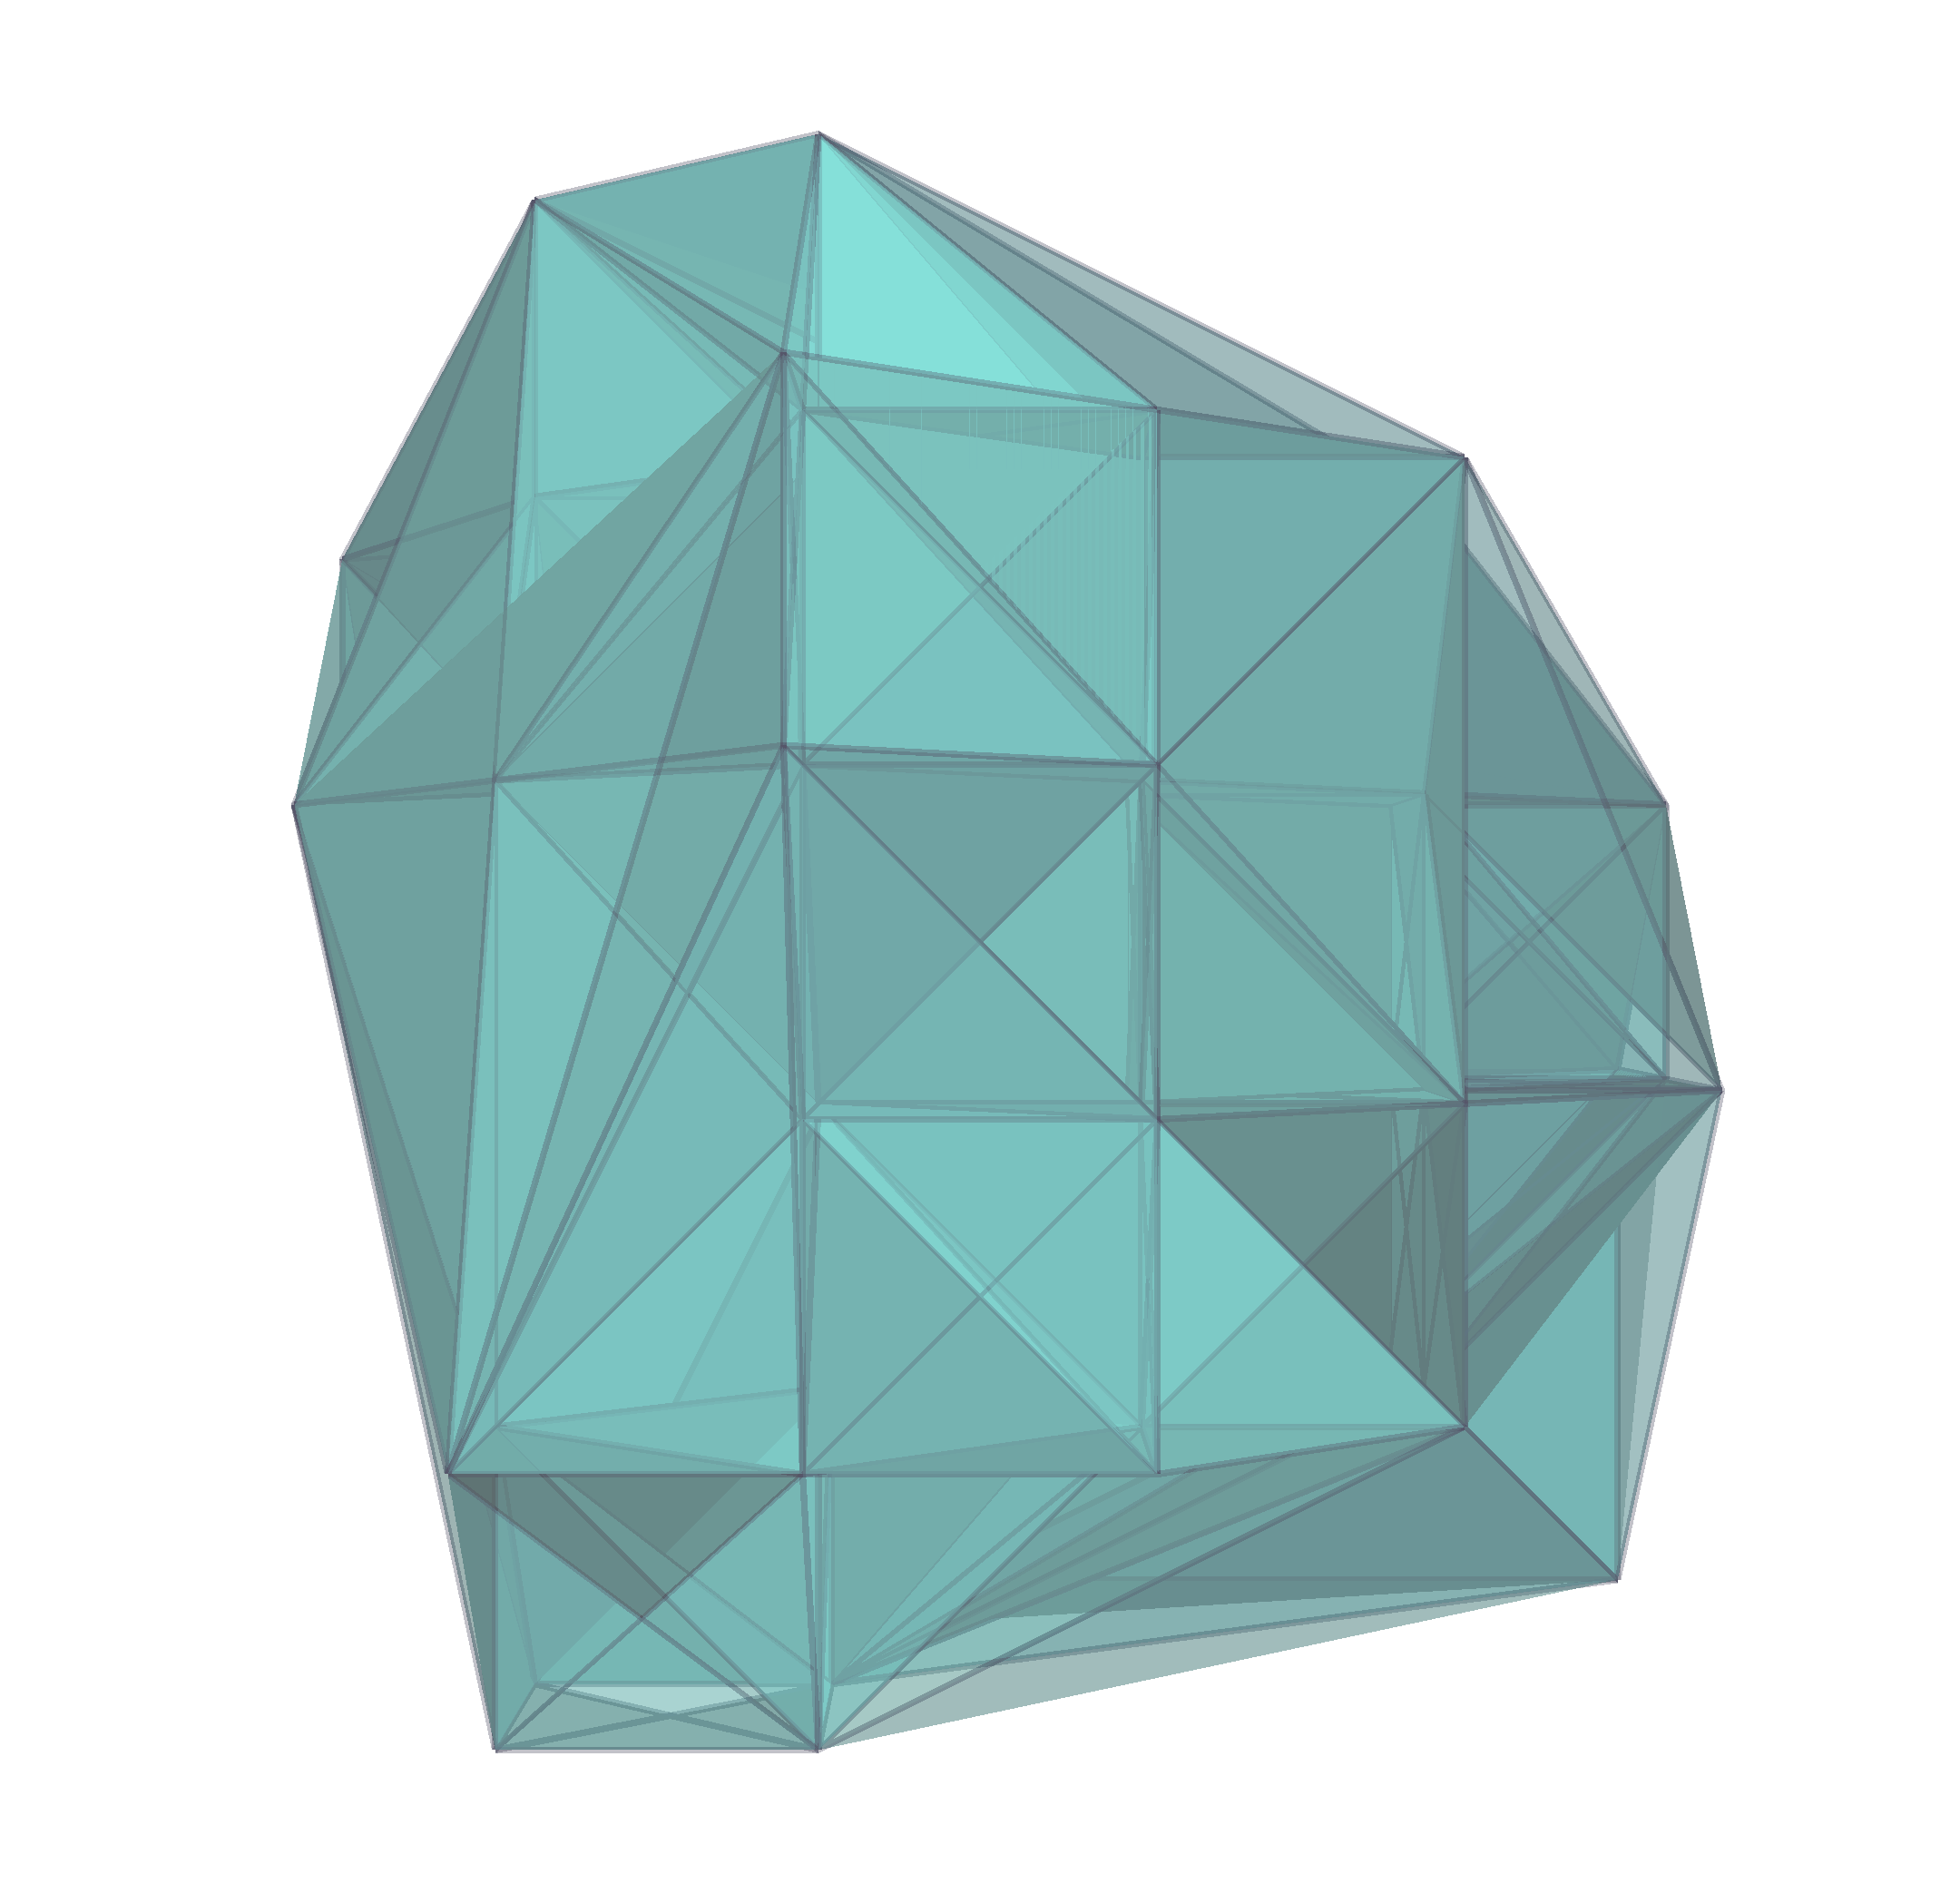
\includegraphics[width=8cm]{Chapter2/Plots/qDel.png}
\centering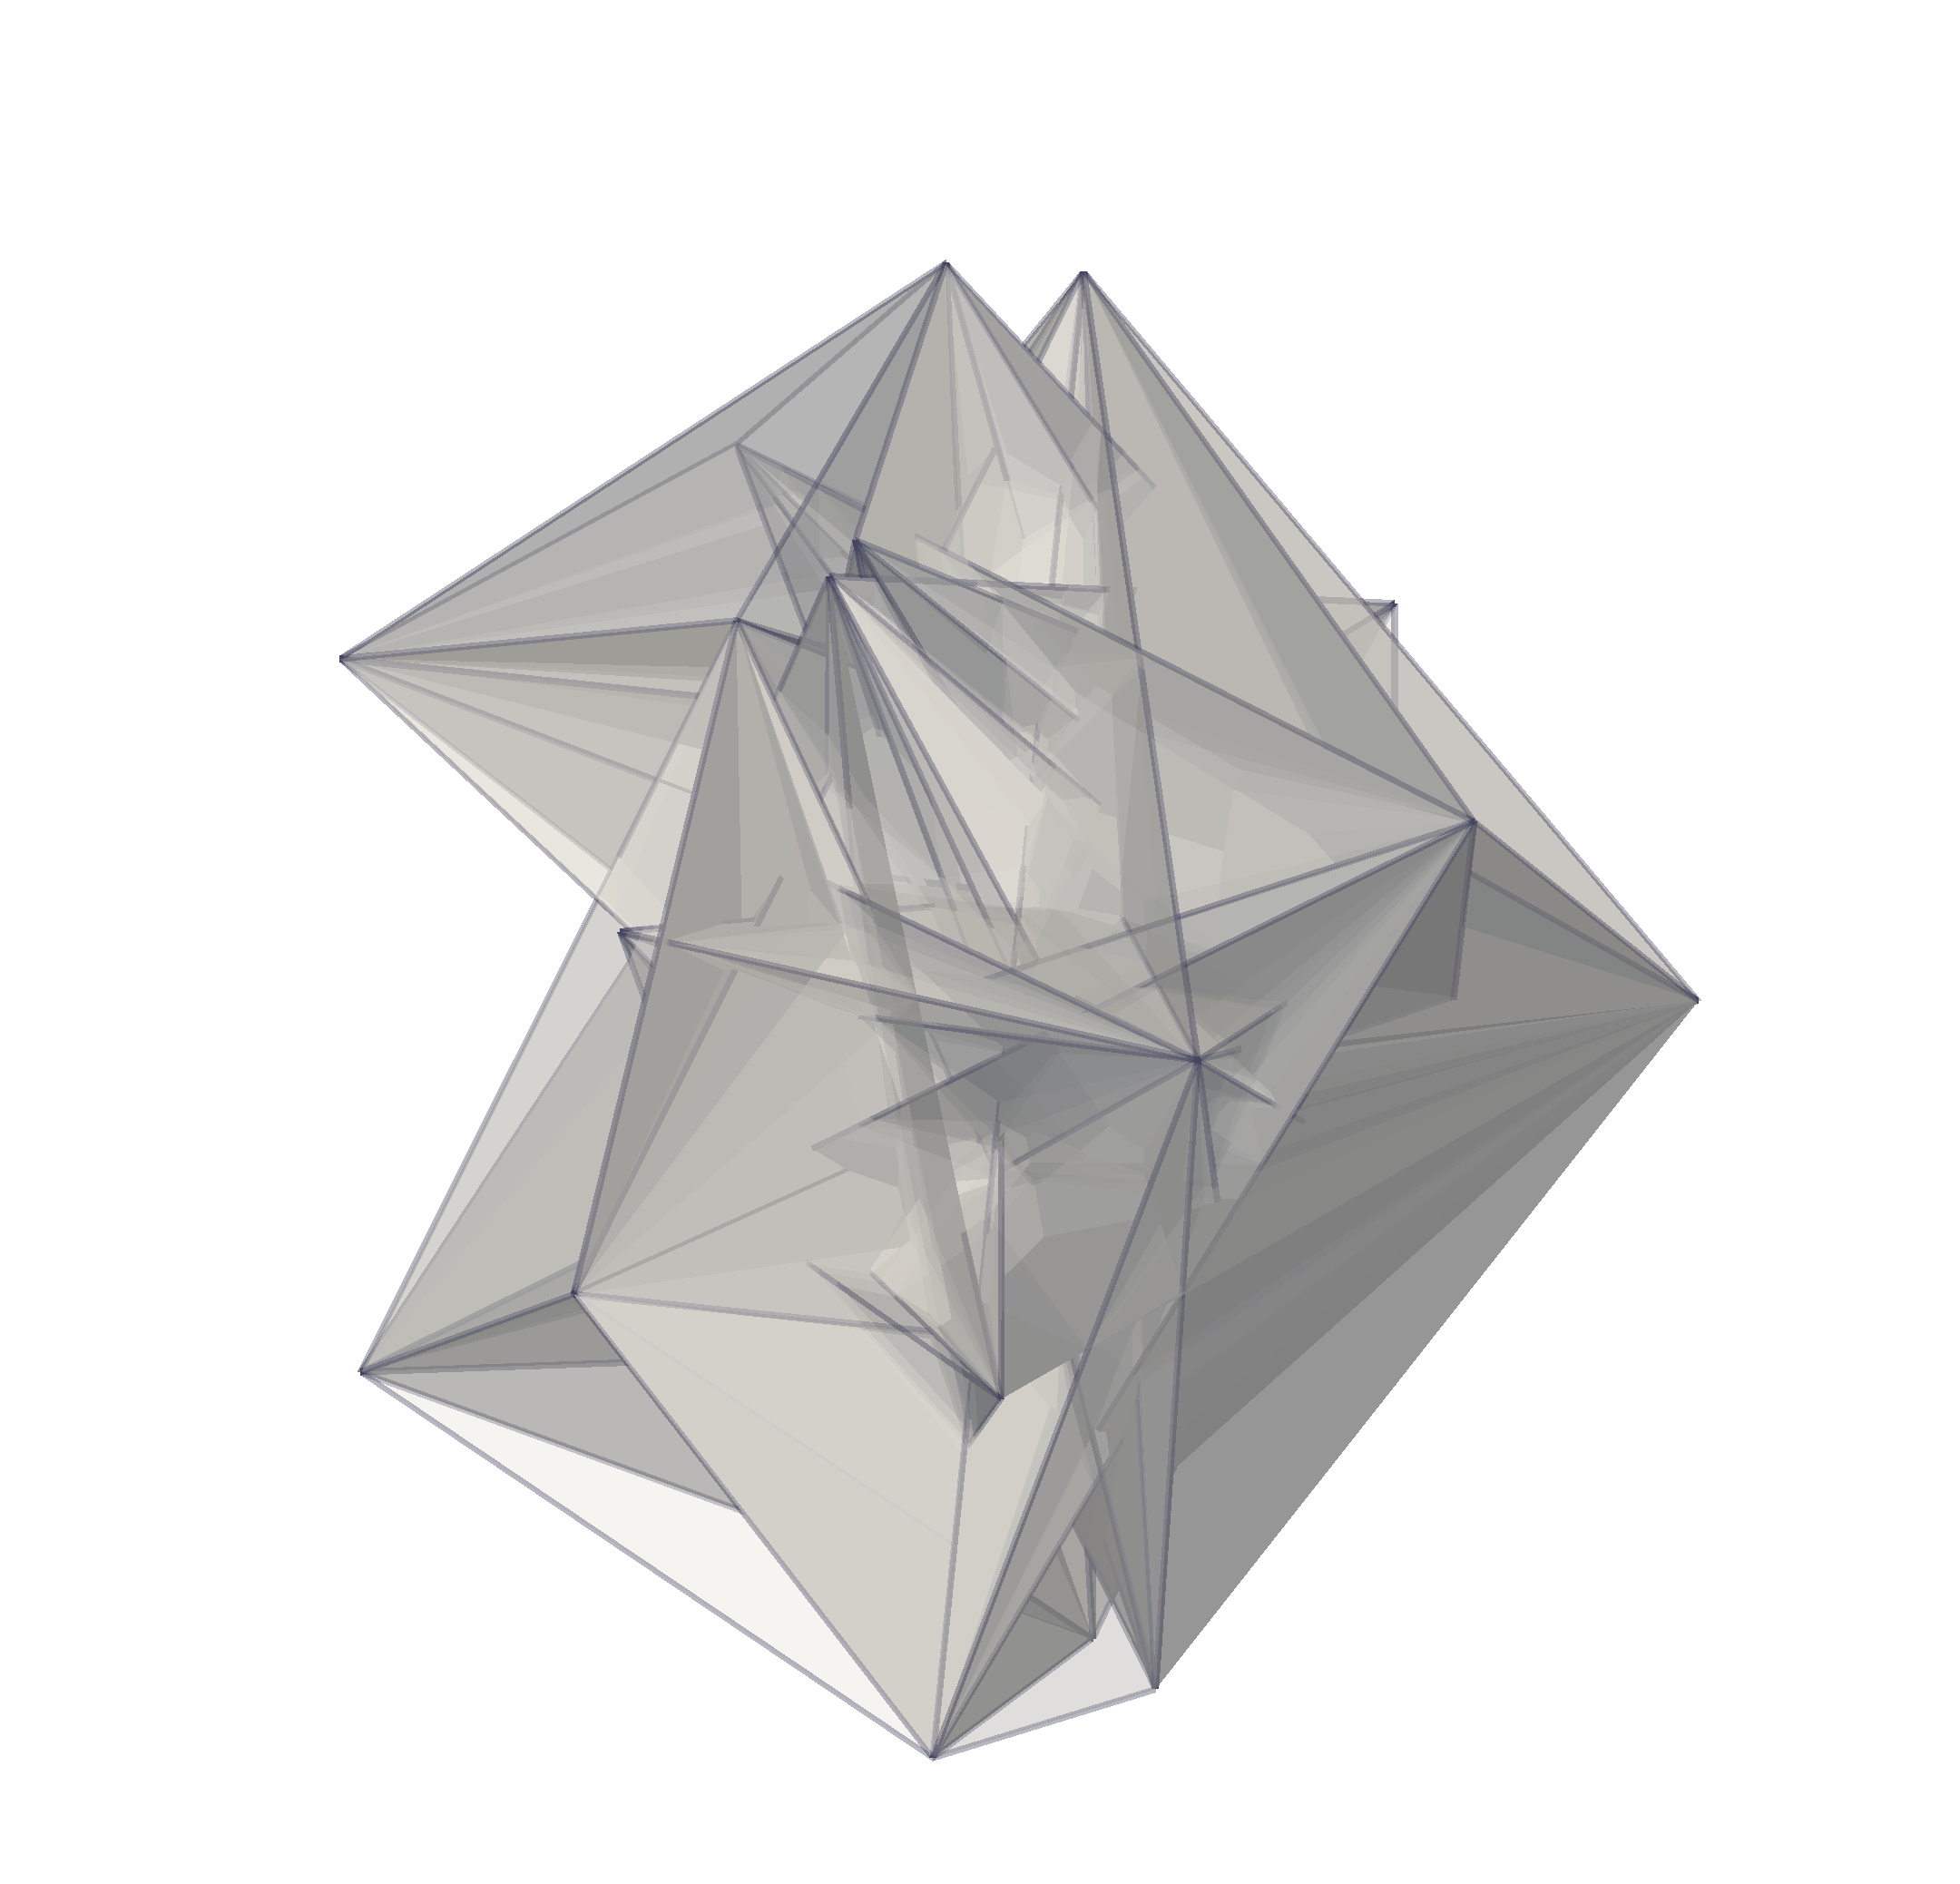
\includegraphics[width=6cm]{Chapter2/Plots/x.png}
\caption{ This plot shows the idea of Lagrangian tessellations. Left: The distribution of Dark matter particles in Lagrangian space is on the regular grid. The tetrahedra surfaces in this case are mostly regular (except at the edges). Right panel shows the Eulerian positions of the same particles at $z=0$. The particles clearly have undergone multiple flip-flops, and the intersections of Lagrangian tetrahedra signifies locations of caustic surfaces. Specific tessellation schemes can be utilized separately to identify these surfaces. }
\label{fig:Tess}
\end{figure}


Furthermore, the analytical understanding of these structures are thoroughly complicated: In a 2-dimensional ZA, for example, there are only two types of fundamental singularities that exist at generic instants of time($A_2$, which are lines and $A_3$, which are the cusp points of $A_2$ lines).   In addition there are two singular points ($A_4$, and $D_4$) that exist  only at particular instants of time: at $A_4$ two cusp $A_3$-points are formed and a smooth part of an $A_2$ line is  transformed in self-crossing
line. In addition there are several transient forms that exist only 
at particular times.
Each of these correspond of formation, mergers, branching and other dynamical processes involving pancakes. \cite{Arnold1982} and \cite{Hidding2014} studied of singularities in 2-dimensional collapse) in exhaustive detail, but similar analytical characterization of 3-dimensional ZA has not been satisfactorily done yet.  
 
 
Complexities in 3-dimensional caustics is partly due the intricate mapping in the hypersurface $\mathbf{x}(\mathbf{q})$ called the Lagrangian submanifold (See Figure \ref{fig:Tess}). The Lagrangian submanifold $\mathbf{x}(\mathbf{q})$  is a single valued, smooth and differentiable function in it's 6-dimensional space $(\mathbf{q}, \mathbf{x})$, however the projection onto 3-dimensional Eulerian space is entangled with creases, kinks and folds (Note that this  submanifold is very different than the phase space $(\mathbf{x},\mathbf{v})$, even though they are connected by a cannonical transformation). However, dilineating the Lagrangian submanifold reveals several properties of the dark matter dynamics not inferred from position-space analyses. Two fields related to tessellating the Lagrangian submanifold -- The Multistream field $n_{str}(\mathbf{x})$ in Eulerian space and the Flip-Flop field $n_{ff}(\mathbf{q})$ in Lagrangian space (check \cite{Shandarin2012}, \cite{Ramachandra2015}, \cite{Shandarin2016}) are closely related. 





\section{The multistream flow field in one-dimension}
% Taken from appendix A
\label{appendix:nstream}

\begin{figure}
\begin{minipage}[t]{.99\linewidth}
  \centering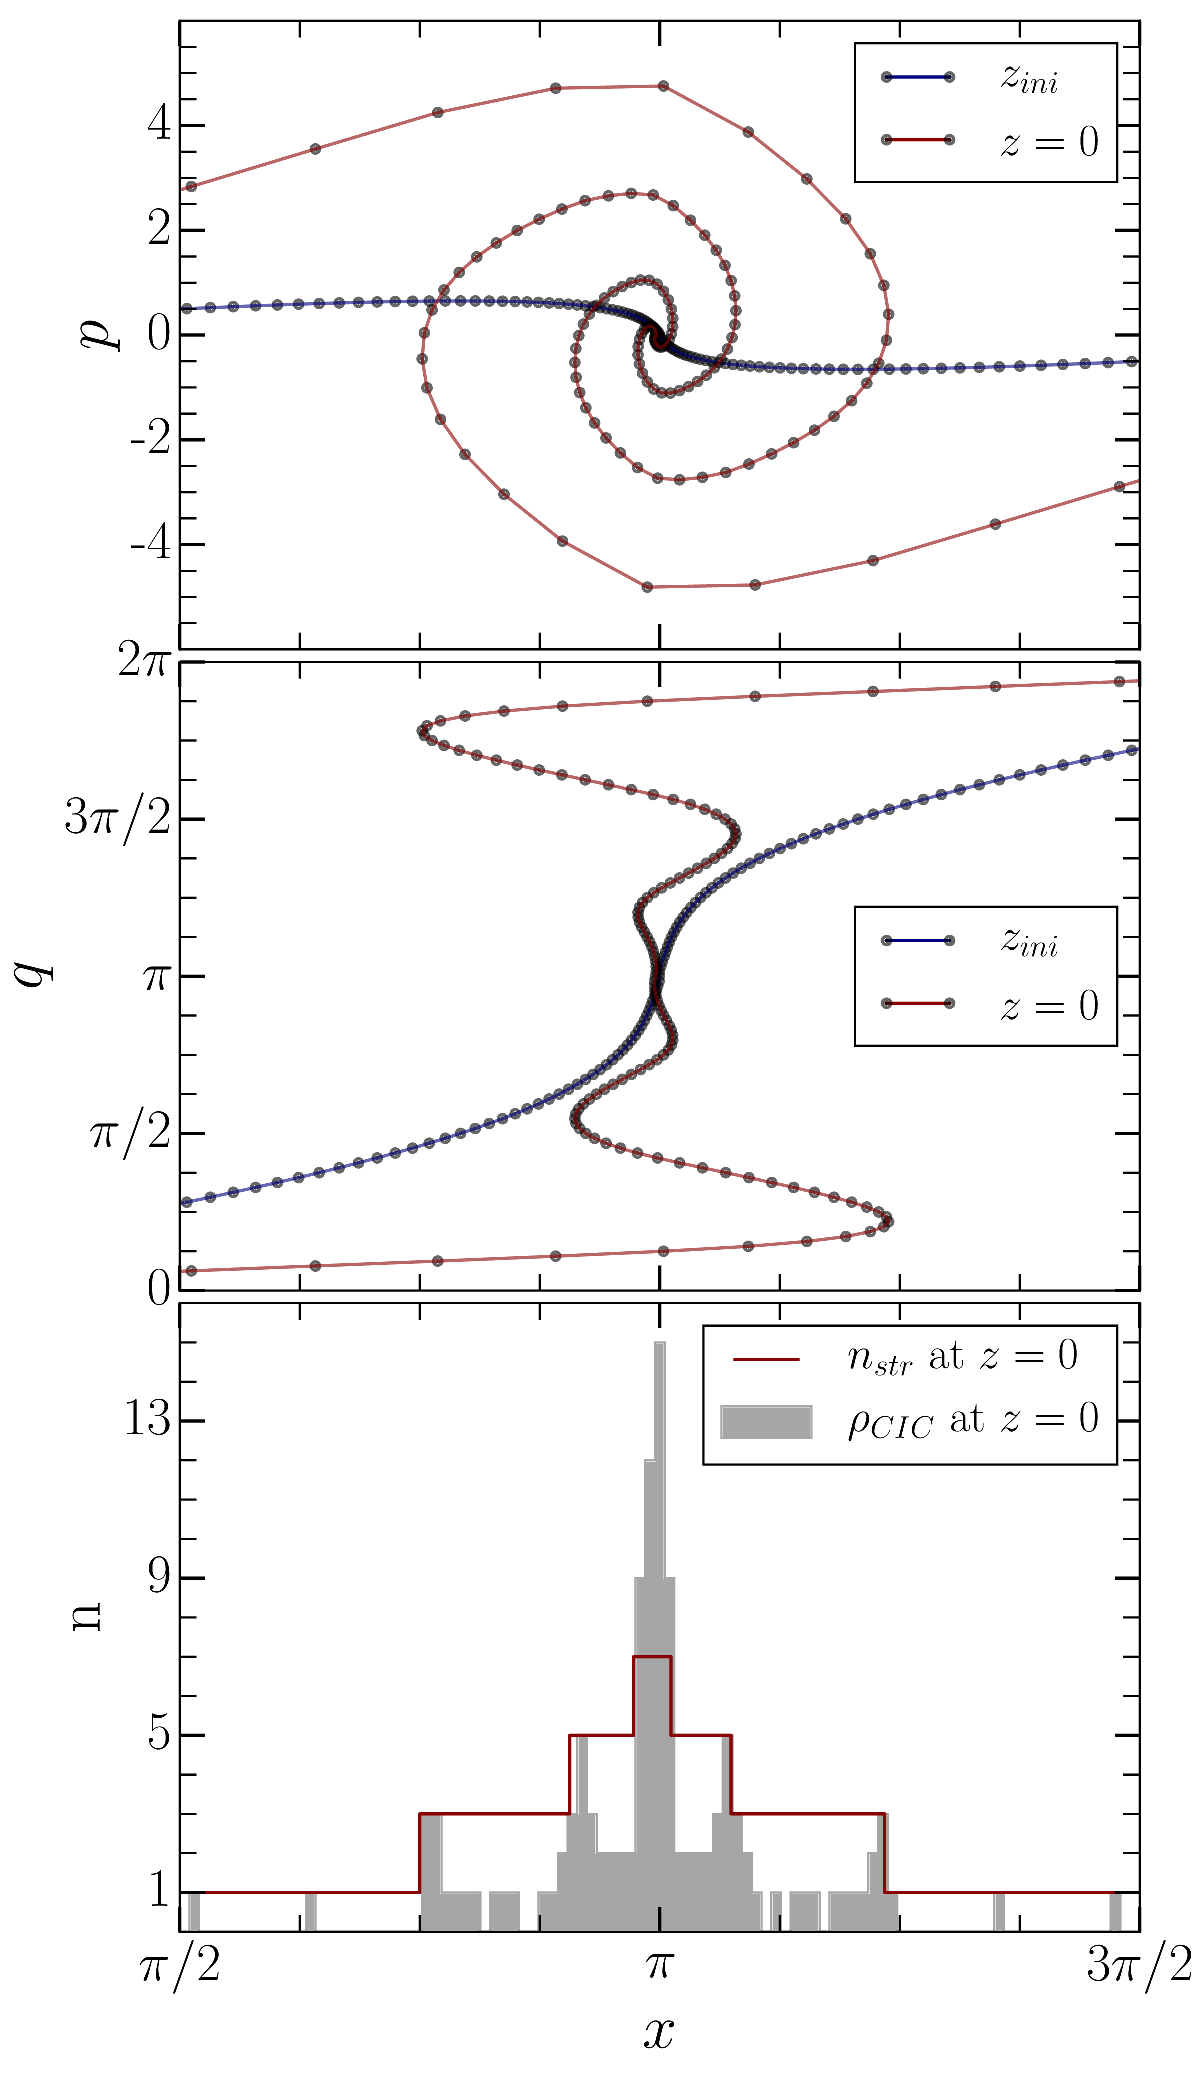
\includegraphics[width=8.cm]{Chapter4/Source_v2/fig13.pdf} 
\end{minipage}\hfill
\caption{ Multi-streaming in one-dimension gravitational collapse. Top panel: $(\bf{p}, \bf{x})$ phase-space representation redshift $z_{ini}$ and $z = 0$. Dots represent the dark matter particles. Initially the mass particles are in the linear stage of evolution. At $z = 0$, multiple values of $\bf{p}(\bf{x})$ is seen in the collapsed regions. Middle panel: Equivalent Lagrangian sub-manifold $\bf{q}(\bf{x})$. At $z_{ini}$, the dashed line represents $\bf{q} = \bf{x}$. Number of streams are parametrized from this sub-manifold. Bottom panel: The multistream field $n_{str}$ and the number-density using CIC algorithm, $n_{CIC}$ at $z = 0$. }
\label{fig:phase1d}
\end{figure}

The top panel in \autoref{fig:phase1d} shows the velocity multistreaming phenomenon in a one-dimensional collapse. The phase-space $(\bf{p}, \bf{x})$ (where $p$ is the momentum and $x$ is the co-moving Eulerian coordinate) is single-valued in the linear stage of evolution (at redshift $z_{ini}$). Non-linear stage of gravitational evolution of the collision-less dark matter particles then results in multi-valued $\bf{p} (\bf{x},z)$ at $z = 0$. The mass particles are sparsely  distributed outside the region of gravitational collapse, and are denser in the inner streams.

 
A dynamically equivalent transformation $(\bf{p}, \bf{x}) \mapsto (\bf{q}, \bf{x}) $ (where $\bf{q}$ is the Lagrangian coordinate) shows the Lagrangian sub-manifold in the middle panel of \autoref{fig:phase1d}. This two-dimensional phase-space has foldings that correspond to multiple velocity streams, although the sub-manifold itself remains continuous. A projection of the Lagrangian sub-manifold at each point in the configuration space quantifies the number-of-streams. Folding in the sub-manifold are checked for points in configuration space using tessellations. The tessellating simplices in one-dimensional model are just the line-segments whose nodes are the dark matter particles in the Lagrangian space. Dynamical property is accounted for in this phase-space tessellation since labels of the nodes remain intact throughout the evolution; the line segments may shorten, extend or change orientation. Each folding in the Lagrangian sub-manifold increases the number of streams by a factor of two. In three-dimensional simulations, the sub-manifold twists in complicated ways in a six-dimensional phase space. The number-of-streams in N-body simulations (\citealt{Shandarin2012} and \citealt{Abel2012}) is calculated using Lagrangian/phase-space tessellations. This triangulation is conceptually different from the Voronoi (See \citealt{Schaap2000} and references therein) or Delaunay \citep{Icke1991} tessellation schemes. 

The bottom panel \autoref{fig:phase1d} shows the the multistream field $n_{str}(\bf{x})$ at $z = 0$. The field only takes the values of 1, 3, 5 and 7 in this scenario. Caustics occur at the folds in Lagrangian sub-manifold, and have a measure zero (study of caustics in one- and  two-dimensional evolution is done in \cite{Hidding2014}, three-dimensional caustic surface in a cosmological simulation is shown in \cite{Ramachandra2017} ). Several properties of the multistream field are significantly different from mass density. The bottom panel also shows an illustration of CIC algorithm (cf. \citealt{Hockney1988}) in calculating density, which is numerically equivalent to counting the number of particles on each cell of a regular grid. One major difference is in the regions before gravitational collapse: $n_{str}$ is universally equal to unity, whereas number density fluctuates. It should also be noted that density by definition is a continuous field; numerical approximations like CIC discretise the field. Alternatively, multistream field is intrinsically a discrete-data field.  



%-------------------------------------------------------------------------------------------------------------------------------
\section{Phase-space representation of gravitational clustering}
\label{sec:HaloFormation}
%% Taken from Paper2017b

\begin{figure*} 
\centering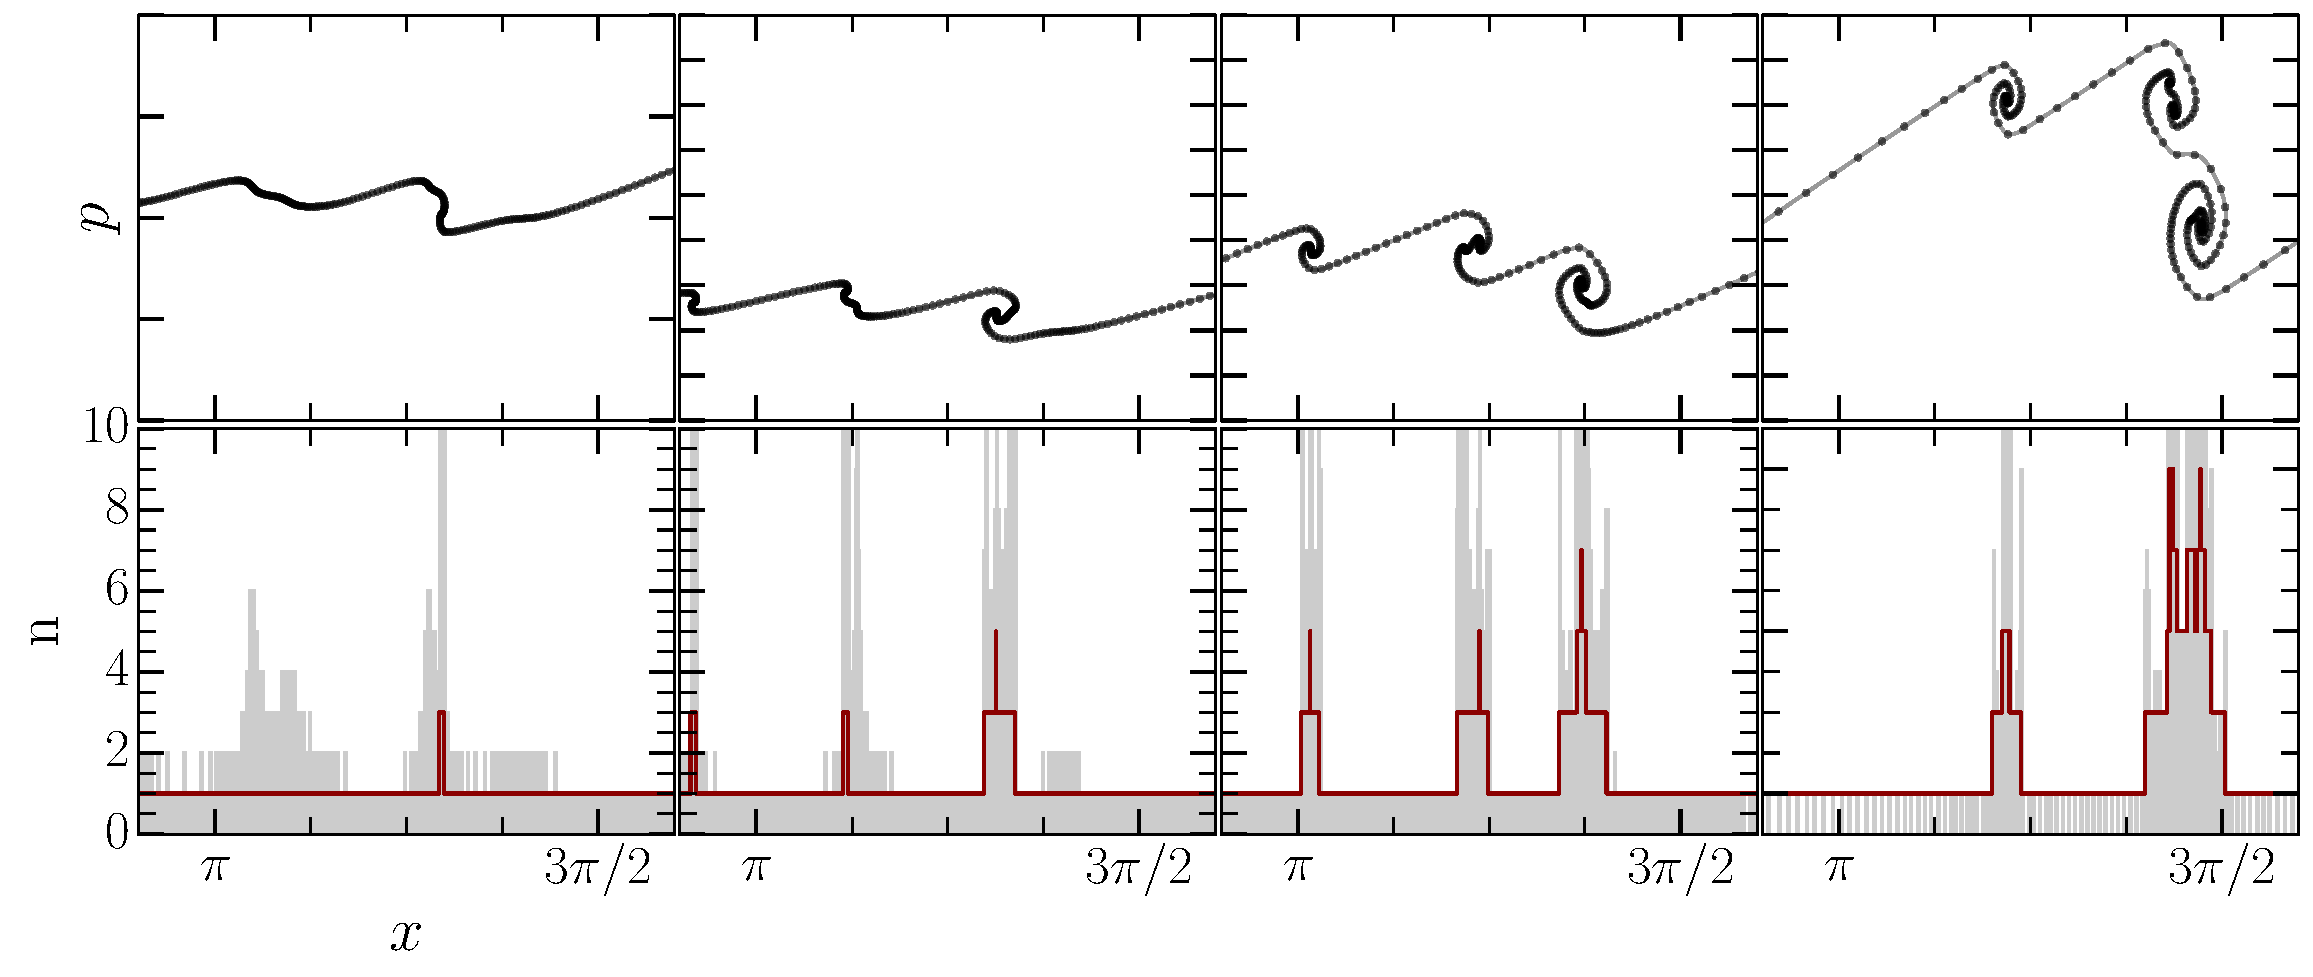
\includegraphics[height=7cm]{Chapter5/Source_v2/fig1.pdf} 
\caption{Dynamical collapse of dark matter in one-dimensional universe: Top panels show the $(\mathbf{p}, \mathbf{x})$ phase-space manifold of the dark matter sheet at redshifts $z_1$, $z_2$, $z_3$ and $z = 0$. Dots represent the dark matter particles. The momentum values are chosen at arbitrary scales. Bottom panels show the corresponding multistream field multistream field $n_{str}(\mathbf{x}, z)$ (red) and density field $\rho(\mathbf{x}, z)$ (gray). }
\label{fig:1d}
\end{figure*}

We begin with a simple illustration showing the formation of a few haloes in a one-dimensional simulation. Dark matter clustering in a (1+1)-dimensional phase-space $(\mathbf{p}, \mathbf{x})$ (where $p$ is the momentum and $x$ is the co-moving Eulerian coordinate) at four successive time steps is shown in the top panels of \autoref{fig:1d}. The lower panels show the corresponding multistream field (\citealt{Shandarin2012} and \citealt{Abel2012}) $n_{str}(\mathbf{x}, z)$ (red) and density field $\rho(\mathbf{x}, z)$ (gray). At $z_1$ (left-most panel), velocity is single-valued in Eulerian co-ordinates shown, except at a small three-stream region near $\mathbf{x} = 5\pi/4$. This is the first instance of multistreaming in the region, which was previously had $n_{str} = 1$ throughout. The interface of $n_{str} = 1$ and $n_{str} = 3$ regions is also the location of the first caustic. On the other hand, the density calculated at a high resolution shows variations, even in the mono-streaming regions. The variations are especially more pronounced around  the caustic (near $\mathbf{x} = 5\pi/4$).


The gravitational clustering is more evolved in the two center panels ($z_2$ and $z_3$) with three prominent phase-space spirals. The regions between the spirals have sparsely distributed dark matter particles, and have $n_{str} = 1$. Each spiral corresponds to a location of gravitational collapse with $n_{str} > 1$ region, and higher density. A few of these regions within three-streaming regions are elevated to $n_{str} = 5$. The corresponding density field is not only noisier, but also reaches very high values at the caustics. This is also a primary distinguishing feature between mass density fields and multistream fields: At the locations of caustic, the density (regardless of how it is calculated) is not smooth \cite{Vogelsberger2011}. Computational limitations on simulation resolutions and refinement of density calculations soften the fields, exceptionally at the zero volume measure regions of caustic surfaces.  On the other-hand, multistream values are increased by finite values at caustic surface locations - This property is preserved at higher simulation resolutions and any refinements of multistream field calculations - although $n_{str}$ may be resolved enough to have intermediate even-values. Multistream fields are also intrinsically discrete valued, which is not true with density fields. Discreteness of multistream fields is discussed in more detail in \cite{Ramachandra2017}. 

The right-most panel in \autoref{fig:1d} shows the final structure at $z=0$. Two large spirals have spatially merged. These collapse environments are naturally very complex, with an increased number of successive caustic formation and merging. 
The corresponding velocity streams also show a more complicated structure. Clearly, the multistream field has a saddle point that is not as low as $n_{str} = 1$. This poses a bigger problem in the context of most of halo detection algorithms, and we discuss this in Appendix \ref{appendix:Eigen}. 



\subsection{Collapse in higher dimensions}

Extending the above results of one-dimensional collapse into higher dimension is vital, primarily in the context of halo formation. The individual spiral collapses in the one-dimension happen at a small region (left-most panel in \autoref{fig:1d}), and the region grows by volume, whilst increasing the spiral twists within. This is in contrast with the theoretical top-hat spherical model of halo formation when the shell crossing would not happen until the final moment of the collapse of the entire halo into a point-like singularity. Thus all shell crossings happen at a single point
and at a single instant of time. The collapse of an isolated, spherically symmetric density peak is a very exceptional case, because every spherical shell feels only the force due to interior mass until it collapses into the caustic region. The collapse of the real peak proceeds in the field generated by the mass distribution - in both the mass within the forming halo, and the mass outside the halo. 

The collapse of a uniform ellipsoid also results in a simultaneous collapse of the entire ellipsoid
however this time not into a point but into a two-dimensional ellipse (\citealt{Lin1965a}, \citealt{Icke1975}, \citealt{Eisenstein1995}).
Another customarily used spherical model of halo formation by \cite{Fillmore1984} and \cite{Bertschinger1985} does not consider
the initial collapse at all. Instead it assumes self-similar initial conditions and the halo at advanced stage with formally infinite number of spherical caustic shells.

The `core' in a collision-less dark matter collapse (in \autoref{fig:1d}) is a region where a multistream region is first formed due to caustic formation. This is conceptually similar to a shell crossing. However, there are successive caustic formations that follow the first shell crossing, and they are not limited to the halo cores. Each caustic increases the multistream value within by a finite number. The cores of the multistream haloes obviously have the local maxima of velocity streams in Eulerian coordinates. On the contrary, mass densities have infinite values at the caustics surfaces, including the core. Discontinuities in densities at these regions of sharp multistream transitions are clearly seen if the mass and spatial resolutions were sufficiently high( see two-dimensional simulations by \citealt{Melott1989} as well as in three-dimensional simulations by \citealt{Hahn2013}, \citealt{Angulo2016}, \citealt{Hahn2016a} etc.). 

\begin{figure} 
\centering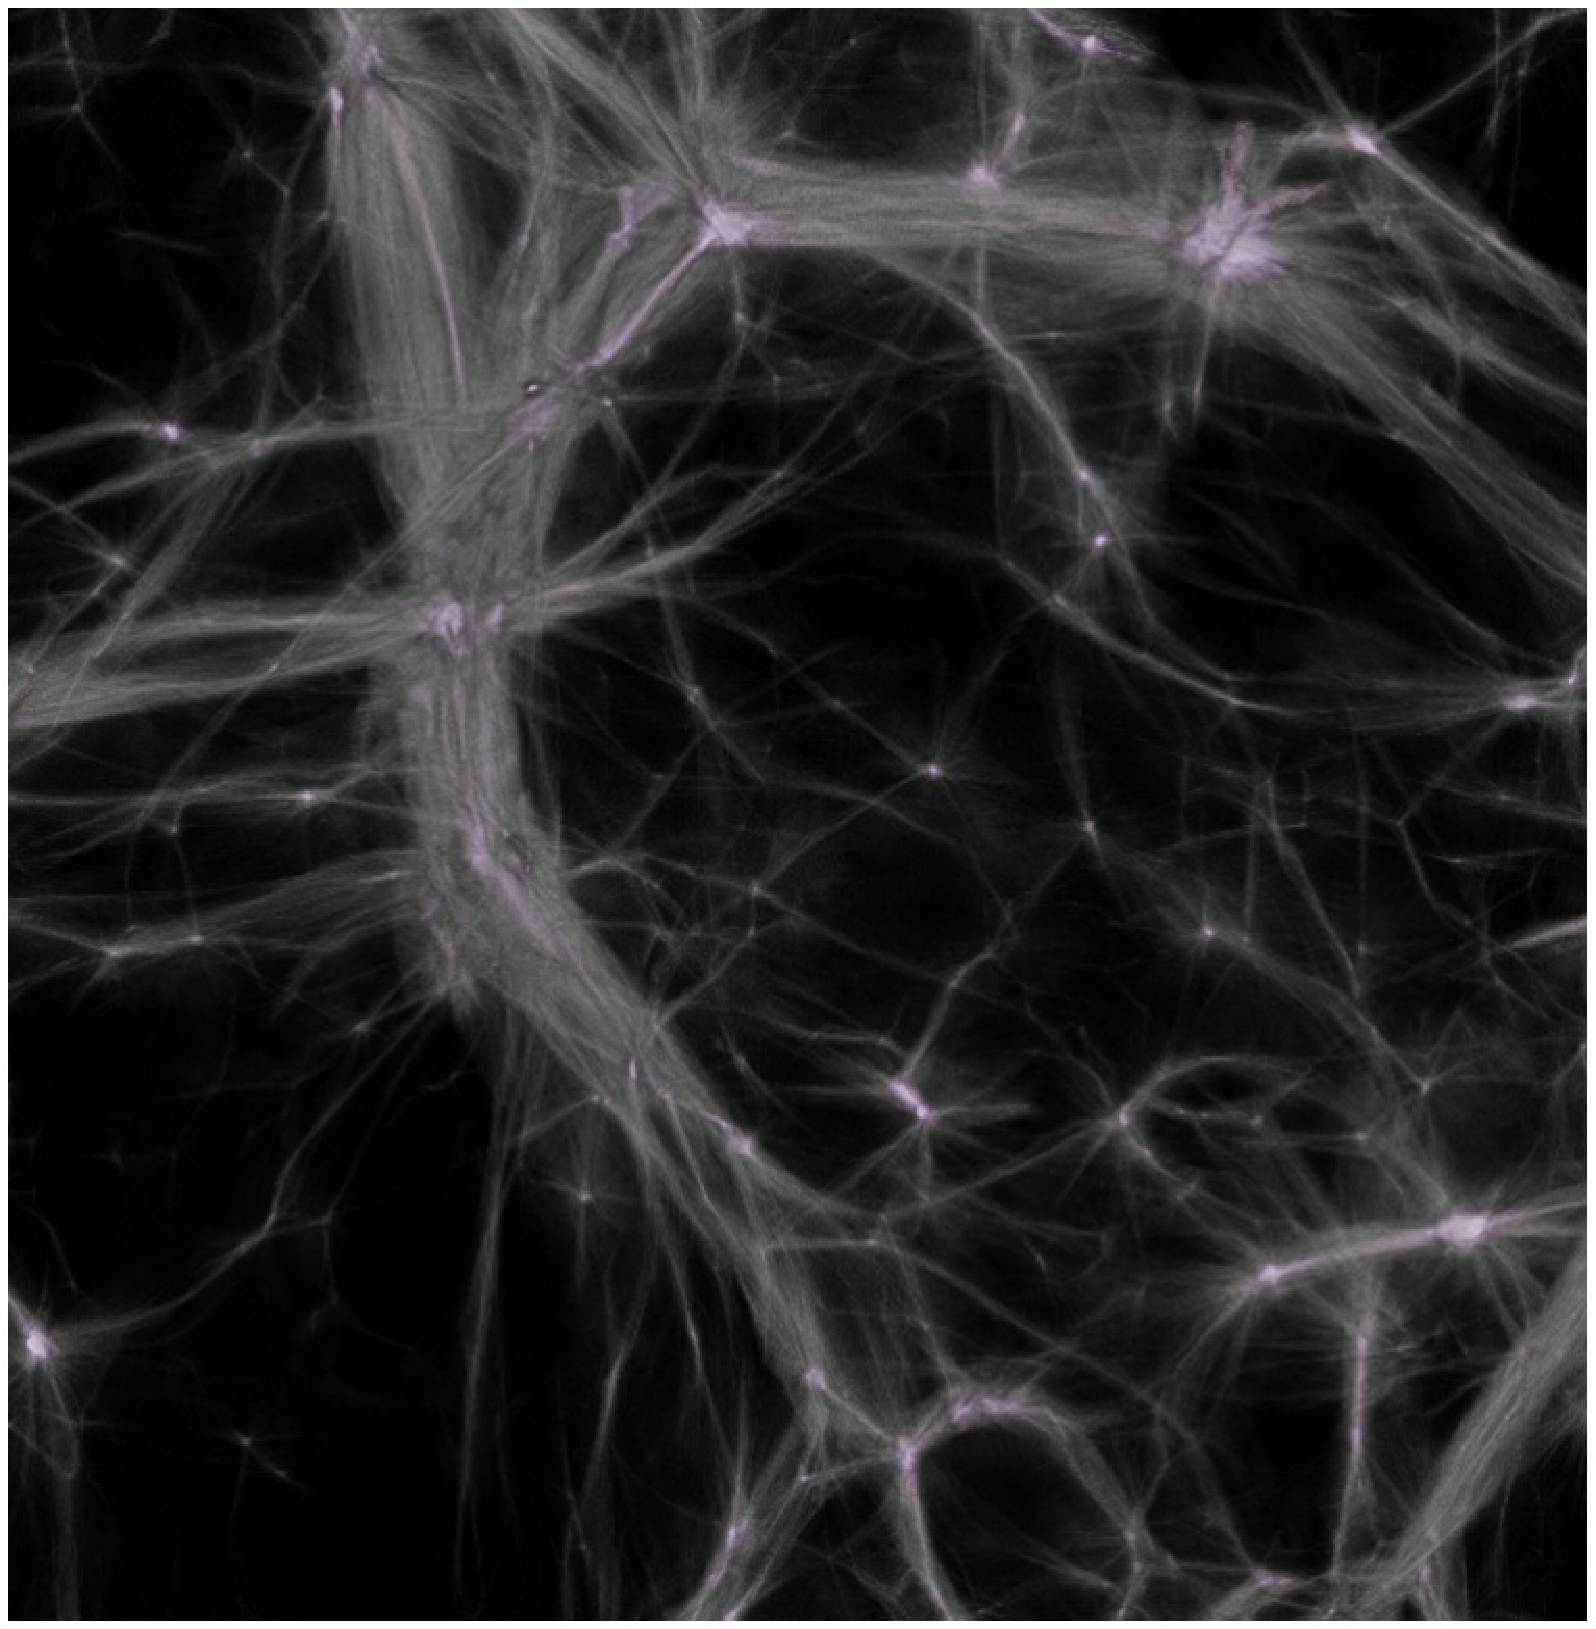
\includegraphics[width=16cm]{Chapter4/Source_v2/fig1.pdf} 
\caption{3D rendering of the multistream field: the cosmic web structure of a $ 50 h^{-1} \text{Mpc} \times 50 h^{-1} \text{Mpc} \times 50 h^{-1} \text{Mpc}$ slice in a simulation box of side length $100 h^{-1}$ Mpc and $128^3$ particles. The multistream field is calculated at 8 times the native resolution. void(black) is a percolating structure with $n_{str} = 1$. Regions $n_{str} \geq 17$ show a filamentary structure (gray) and the bright spots at the intersections of the filaments are regions with $n_{str} \geq 100$. }
\label{fig:full_3d}
\end{figure}

In three-dimensional simulations, the Lagrangian sub-manifold twists in complicated ways in a six-dimensional phase space. This is due to complexities involving caustic formations in higher dimensions, which is true even in the ZA, see \citealt{Arnold1982} and \citealt{Hidding2014} for detailed analyses of caustic formation. The resulting intricate geometrical structures can be characterized by the $n_{str}$ field. Nearly  $90\%$ of the volume in N-body simulations are single-streamed voids at $z=0$ (\citealt{Shandarin2012}, also see \citealt{Falck2015} for a percolation analysis of single-streaming voids). From the visualizations in \cite{Ramachandra2015} and percolation analysis of \cite{Ramachandra2017}, we also know that the $n_{str} = 3$ regions mostly form connected wall-like structures (also see \autoref{fig:full_3d}), unlike the isolated patches as seen in one-dimensional simulations of \autoref{fig:1d}. The structures become predominantly filamentary at higher thresholds of $ n_{str} \gtrsim 17$. Subsequently, the regions around the multistream maxima have isolated closed surfaces (for example, in \autoref{fig:full}), which may be identified as halo locations. 



\begin{figure} 
\centering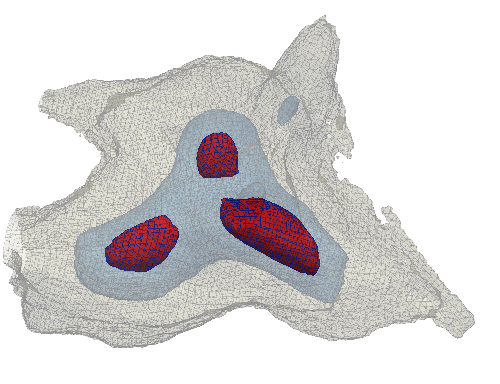
\includegraphics[width=11cm]{Chapter5/Source_v2/fig2.pdf} 
\caption{Multistream field contours: The multistream field is calculated at 8 times the native resolution. Each inner convex blobs (red) surround local multistream maxima inside. Surrounding outer shell(blue) is not convex throughout the surface, and the outermost gray multistream surface displays a filamental geometry.}
\label{fig:full}
\end{figure}


Caustic formations and mass accretion are also seen to occur more along the higher streams, which makes the haloes non-spherical, with the alignment generally determined by a complicated interplay  of the intensities of the streams from neighboring filamentary structures. Number of streams corresponding to the dark matter halo also has a local environment dependence. The three small haloes in \autoref{fig:full}, where the number of streams are higher than the neighbouring filaments, are aligned along three intersecting filaments. Halo environment studied in \cite{Ramachandra2015} show similar hierarchical variation in $n_{str}$ values. The halo environments are thus very complicated, and empirical thresholds (on multistream or density fields) may not account for all the haloes uniformly. Hence we use a local geometrical method to identify potential haloes in multistream fields.


The first non-linear structures in the web have $n_{str} = 3$. By visual inspection, these regions generally form a fabric-like open structures that resemble walls. The surface contours of higher $n_{str}$ are embedded within the walls. \autoref{fig:full_3d} shows a filamentary structure of the web at $n_{str} \gtrsim 17$. The figure also shows regions around local maxima of the multistream field, which are generally located at the intersections of filaments.    








% % \section{Dynamics: Lagrangian sub-manifold}
% Multi-stream flows, Caustics, Flip-flips
\begin{comment}
\documentclass[useAMS, usenatbib]{mn2e}

\pdfoutput=1 

\pdfminorversion=5 

\setlength{\hoffset}{0.5in}
\setlength{\voffset}{-0.5in}

\newcommand{\aap}{A\&A}
\newcommand{\apj}{ApJ}
\newcommand{\mnras}{MNRAS}
\newcommand{\prd}{Phys. Rev. D}
\newcommand{\sovast}{Soviet Astronomy}
\newcommand{\nat}{Nature}
\newcommand{\jcap}{Journal of Cosmology as Astroparticle Physics}
\newcommand{\araa}{Annual Review of Astronomy as Astrophysics}

\input{epsf}

\usepackage{amssymb, amstext, amsmath, epsf, graphicx, graphics, epsfig, wrapfig, listings, float, esint}
\usepackage{hyperref, natbib, ifthen}


% ----------------------------------------------HIGHLIGHTING --------DELETE--------------
\usepackage{xcolor}
\usepackage[normalem]{ulem} % use normalem to protect \emph
\newcommand\hl{\bgroup\markoverwith
  {\textcolor{yellow}{\rule[-.5ex]{2pt}{2.5ex}}}\ULon}
  

%-------------------------------------------------------------------------
%-------------------------------------------------------------------------
\begin{document}



\title[Paper 1]{Multi-stream portrait of the Cosmic web}

\author[Ramachandra \& Shandarin]
	{Nesar S. Ramachandra, \thanks{E-mail: nesar@ku.edu} 
	Sergei F. Shandarin, \\
	Department of Physics and Astronomy, University of Kansas, Lawrence, KS 66045}



 \maketitle
%-------------------------------------------------------------------------------------------
\begin{abstract}
We report the results of the first study of the multi-stream environment of dark matter haloes in cosmological N-body simulations
in the $\Lambda$CDM cosmology. The full dynamical state of  dark matter can be described as a three-dimensional sub-manifold
in six-dimensional phase space - the dark matter sheet. In our study we use a Lagrangian sub-manifold ${\bf x} = {\bf x}({\bf q},t)$ 
(where {\bf x} and {\bf q} are co-moving Eulerian and Lagrangian coordinates respectively), which 
is dynamically  equivalent to the dark matter sheet but is more convenient for numerical analysis.
Our major results can be summarized as follows. At the resolution of the simulation i.e. without additional
smoothing, the cosmic web represents a hierarchical structure: each halo is embedded in the filamentary framework of the web predominantly 
at the filament crossings, 
and each filament is embedded in the wall like fabric of the web at the wall crossings. 
Locally, each halo or sub-halo is a peak in the number of streams field. The number of streams in the neighbouring  
filaments is higher than in the neighbouring walls. The walls are regions where number of streams
 is equal to three or a few. Voids are uniquely defined by the local condition requiring to be a single-stream flow region.
  The shells of streams 
 around haloes are  quite thin and the closest void region is typically within one and a half FOF radius 
 from the center of the halo.
\end{abstract}

\begin{keywords}
methods: numerical -- cosmology: theory -- dark matter -- large-scale structure of Universe 
\end{keywords}
\end{comment}

\chapter{Multi-stream portrait of the Cosmic web}\label{chapter3}


In this chapter, we report the results of the first study of the multi-stream environment of dark matter haloes in cosmological N-body simulations in the $\Lambda$CDM cosmology. We arrive at heuristic parameters for delineating walls, filaments and haloes in the multi-stream web, while single streaming regions are simply devoid of gravitational collapse, i.e., are voids. The results in the chapter were first discussed in \cite{Ramachandra2015}. 


\section{Brief introduction} \label{sec:3intro}



The problem of objective identification and quantitative characterization of anisotropic structures 
in the distribution of galaxies in space emerged after the first evidences of their existence
(see the review by \citealt{Oort1983} and the references therein). The first theoretical model predicting highly anisotropic concentrations in the mass distribution coming into existence at the non-linear stage of gravitational instability is known as the Zel'dovich Approximation (the ZA) (\citealt{Zeldovich1970}, for further developments see also \citealt{Shandarin1989} and the references therein). The ZA predicted the formation of  `pancakes'  also known as the walls in the currently popular jargon. The later development
of the model by \citet{Arnold1982} predicted the formation of filaments along with the pancakes. \citet{Klypin1983a} and \citet{Shandarin1984} demonstrated that the filaments emerge in the cosmological N-body simulation in three-dimensional space.
However, they failed to identify the pancakes at $z=0$. Both the existence of filaments connecting compact clumps of matter and absence of pancakes were confirmed by \citet{Frenk1983}. Puzzled by the absence of the pancakes \citet{Klypin1983a}
speculated that insufficient mass resolution of the simulation was the cause  of the negative outcome. 
This has been unambiguously confirmed by recent simulations using a better numerical technique of computing a density field from the particle
coordinates in cosmological N-body simulations (~\citealt{Shandarin2012} and ~\citealt{Abel2012}). \citealt{Klypin1983a} 
also stressed that the most of filaments are  incorporated in 
`a single three-dimensional web structure'\footnote{The term `cosmic web' was coined by  \citet{Bond1996}.}. 
They admitted that
their simulation did not allow them to confirm the existence of pancakes between the filaments predicted by the ZA \citep{Arnold1982}.

  
Although the four archetypal elements of the cosmic web:  voids, walls/pancakes, filaments and haloes 
were predicted by ZA and confirmed in cosmological N-body simulation their identification and quantitative characterization
remains under vigorous debate
(see e.g. \citealt{Colberg2008}, \citealt{Elahi2013}, \citealt{Knebe2013}, \citealt{Hoffmann2014}).
The dark matter haloes are arguably the easiest objects to identify in N-body simulations. They can also be reliably associated with
observed objects like galaxies and clusters of galaxies.  But even in this case \citet{Knebe2013} refer to almost thirty different
halo finders suggested after 2000. Identifying filaments and pancakes/walls is far more controversial in both N-body simulations 
and galaxy catalogs. For instance, even estimating the global parameters of the  web  in N-body simulation such as the fractions of volume and mass
in voids, walls/pancakes, filaments and haloes produced quite different results. The estimates of volume 
fractions of voids range from 13  to 86\%  (\citealt{Cautun2014a}, \citealt{Falck2015}, \citealt{Forero-Romero2009a} , \citealt{Hahn2007} , \citealt{Aragon-Calvo2010a}). Similar estimates for walls/pancakes, filaments 
and haloes  are respectively 5-56\% 2-26\% and 0.1-1\%.  Estimates of the mass content vary in large ranges as well.

Large differences in the estimates of volume and mass fractions made by different groups are not surprising if we recognize
considerable differences in the definitions of the components of the cosmic web and numerical methods used in the estimates. Without trying to provide an exhaustive review of all definitions and techniques used for the quantitative morphological 
analysis of the web  we just briefly describe a few approaches in order to illustrate how different they could be. 
Some groups study the web morphology using only coordinates of simulation particles, while others use the particle velocities too. 
Transforming data from  point sets to the density and other fields on a grid is also often used
because fields allow to use a variety of mathematical techniques not available for the particle sets.
However this step can be done by a variety of methods some as simple as cloud-in-cell (CIC), or more complicated as smoothed-particle hydrodynamics (SPH), 
or using Voronoi and Delaunay tessellations
as in the Delaunay Tessellation Field Estimator (DTFE) method (~\citealt{Weygaert2009}, \citealt{Cautun2014a}).  
Recently a new method called a discrete persistent structure extractor (DisPerSE \citealt{Sousbie2011f},  \citealt{Sousbie2011e} allowing to identify haloes and other components of the web directly from the particles 
has been designed.  This method can be applied to the galaxy catalogs, for instance \citet{Sousbie2011e} applied it to SDSS catalog and extracted the filaments (which are made available online).

An obvious advantage of methods based on particle coordinates, both based on the density field and directly on particle coordinates, is their applicability to redshift catalogs. 
The redshift catalogs like SDSS and 2dF provide only two angular coordinates and distances in redshift space. 
But cosmological N-body dark matter simulations provide the full dynamical information in six-dimensional
phase space. This additional information is very valuable providing a greater opportunity for understanding the 
physics of the web and developing a better theory of the web.

Dark matter distribution in phase space is highly degenerate because it is cold. 
Practically, it occupies a three-dimensional sub-manifold in six-dimensional phase space.
 In the linear regime, the dark matter sub-manifold is a single-valued function of Eulerian coordinates 
 which means that at each point the dark matter is represented by a single stream flow. As the density perturbations in dark matter grow with time the number of streams jumps to three at the regions of
shell crossing. Then five stream regions emerge inside of the three stream regions and so on.
Number of streams remains an odd integer in generic points.   The corresponding parts of the three-dimensional dark matter sub-manifold 
form complicated folds in six-dimensional  phase space.   

The regions with multi-stream flow constitute the web while the regions with only one stream form
voids (\citealt{Shandarin2011}, ~\citealt{Shandarin2012}, ~\citealt{Abel2012},~\citealt{Falck2012}).
This definition of voids states that in a given N-body simulation, no haloes can be formed before the first
shell crossings have occurred and the smallest haloes cannot be smaller than the mass corresponding 
to the small scale cut-off in the initial power spectrum regardless of the cause of the cut-off:  physical or due to numerical
limitations (see e.g. \citealt{Angulo2013}).  This definition of voids is physical by nature and thus has no  free parameters. In addition, it does not speculate on the sub-grid physical processes.
The first three-stream flow regions are similar to the pancakes in the ZA.
They quickly grow and merge into a complicated three-dimensional structure; filaments making the framework of the web manifest 
themselves at the pancake crossings,  and haloes emerge at the filament crossings. At later times  different parts of the web participating
in the large-scale motion overlap  which increases the web complexity further.

Using the full six-dimensional information allows one to generate new fields which  provide 
additional useful information about the evolution and morphology of the  web. 
One of them is a multi-stream field in Eulerian space, which will be the focus of this chapter. 
Another example is the flip-flop field in Lagrangian space. In cosmological context it was first used in the ZA.
\citet{Vogelsberger2011} used it in a study of multi-stream structure of galaxy size haloes.
\citet{Shandarin2014a} applied it for identifying sub-haloes  in dark matter haloes.
A similar although somewhat simplistic realization of this idea has been revealed in the ORIGAMI method
used for the analysis of the web ( \citealt{Falck2012},  \citealt{Falck2015} ).
 Although these fields cannot be used directly on observational data because the full phase-space information
 is not available, they provide much deeper insight into non-linear clustering of collision-less dark matter
and reveal new features of the web.

%We do not discuss the relation between the multi-stream and density fields here because this issue was discussed in detail in previous
%publications (~\citealt{Shandarin_etal:12} and ~\citealt{Abel_etal:12}).

In order to compute the multi-stream field we will use the tessellation scheme described in
 \citet{Shandarin2012} which is  also briefly discussed in Section \ref{subsec:method}.
  Using this methodology on the entire simulation box, we discuss the global behavior of the number of streams in the cosmic web in Section \ref{sec:global}. 
  The tessellation technique we have utilized can be used to find multi-stream fields in smaller Eulerian boxes with very high resolution too. In Section \ref{sec:local} we study the local behavior of multi-streams flows in regions around haloes the detected using friends-of-friends (FOF) technique.
 
 


\section{The simulation}
\label{sec:3simulation}


We have utilized the data from cosmological N-body simulations by Gadget-2 \citep{Springel2005c} for 100 $h^{-1}$ Mpc  and 200 $h^{-1}$ Mpc box 
sizes with $128^3$, $256^3$ and $512^3$ grids. Each particle is between  $10^9 - 10^{12} M_{\odot}$. 
The initial conditions and cosmological parameters are consistent with the Planck cosmology. We utilize the initial Lagrangian box and do a three-dimensional mapping onto corresponding evolved simulations. In addition, for local multi-stream analyses around haloes, we have utilized halo catalogs for each of these simulation boxes. These haloes are detected using FOF method considering objects with more than 20 particles found at linking length, $ b= 0.2$.  
%-------------------------------------------------------------------------------------------------------------------------------
\section{Multi-stream field calculation}
\label{subsec:method}

Phase space tessellation considers the dynamics of the particles similar to that of a standard N-body code. 
However the particles are nodes of the tessellation, and are just massless tracers of the flow.
Assuming that the uniform state is modeled by a simple rectangular grid, the particles are the nodes of the grid.
Each elementary cube of the grid is tessellated by five tetrahedra (\citealt{Shandarin2012}\footnote{For the description of an alternative type of the tessellation see \citet{Abel2012}.}) of which the vertices are the
vertices of the cube. Mass is assumed to be uniformly distributed within each tetrahedron and the tessellation remain
intact at all times. The tetrahedra of the tessellation change their shapes and volumes, the latter are used for
computing the densities of the tetrahedra. Despite the complicated deformations experienced by the three-dimensional
sub-manifold tessellated by the tetrahedra, it remains continuous. Projected on three-dimensional configuration space, the tetrahedra
may form complicated structures. The number of streams at a chosen point {\bf x} is simply the number of tetrahedra that contain the point. The diagnostic points are computationally convenient to choose on a regular grid which can be significantly finer than the original grid in Lagrangian space. The ratio of separation of particles on the initial unperturbed grid to the separation distance of points in the diagnostic grid  $l_{\rm part}/l_{\rm dg} $ will be referred to as the refinement factor in the rest of the chapter.

Number of streams are odd-valued in the entire configuration space, except in a set of points of measure zero where caustics are formed.  
 A single-stream flow implies that the tetrahedra do not overlap in the corresponding region and thus defined as a void region.
 The web is defined as a set of non-void regions, i.e. the set of regions where the number of stream is equal to or more than three.
 The level of non-linearity in the web  can be quantitatively characterized by using `number of streams' as a parameter. As shown in  \citep{Shandarin2012} there is no simple local relation between the number of streams and density, however the both
 fields are obviously correlated.

%\hl{The boundaries of structures in collisionless cold medium (a thermal velocity rms $\sigma_{th} = 0$) are naturally defined by caustic surfaces where the density is infinite. Crossing a caustic at a generic point results in a change of the number of streams by two.
%The caustic surfaces have neither edges no holes.
%Thus a region with $n_{str}$ is a typically narrow shell between the caustic surfaces separated it 
%from the regions with $n_{str}-2$ and $n_{str}+2$ streams. 
%The picture of caustics in a cold medium becomes more complicated
%in a set of points of measure zero (i.e. on lines and in isolated points) where the regions with 
%$n_{str}-2$, $n_{str}$ and $n_{str}+2$ streams can be in a contact simultaneously. A curious reader may
%find a two-dimensional example of this phenomena in \citet{Hidding_etal:2014}, Fig. 15.
%In a medium with small but finite  $\sigma_{th}$ the caustics are transformed into very
%narrow ridges in the density field. The ridges form thin quasi-two dimensional shells having neither
%edges nor holes.   Two obvious inferences from
%this brief discussion of the structure of the milt-stream field which are most important for understanding 
%of the rest of the paper are as follows. 
%First, before any physical structure can form the number of streams is equal to unity
%and second there is no contact surfaces between the regions with one stream and regions 
%with more than three streams.}

%\citet{Shandarin_etal:12} showed that the volume fraction occupied by
%the regions with a given number of streams is a monotonic fairly rapidly decreasing function:
%approximately $v_f(n_{str}) \propto n_{str}^ {-2.8}$ however as show bellow the exponent  depends 
%---------------------------------------------------------------------------------------------
%---------------------------------------------------------------------------------------------


\section{Global statistics of Cosmic web}
\label{sec:global}

The 3-dimensional multi-stream field for the entire simulation box exhibits cosmic web structure with void, walls, filaments and haloes. We propose the number of streams, `$n_{str}$' as a parameter for characterizing and distinguishing structures in the universe. This is different from \citet{Falck2015}, 
where the authors have identified voids, walls, filaments and haloes by particles which have undergone any number of flip-flops along 0, 1, 2 or 3 axes respectively. 
Their description of voids is close to ours except that some particles that have  experienced no flip-flops might be in the region
of multi stream flow formed by other particles.
Thus we expect that the mass fraction in voids defined as the regions with $n_{str} = 1$ is somewhat lower than that defined as the particles with 
flip-flops $= 0$ only at the final state. This is because some particles may have already fallen in the web but  have not experienced flip flop yet and 
some particles that have experienced an even number of flip flops may come back to the original order. However the above arguments are valid only if the thickness of the web is the same in the both approaches. As we discuss below the thickness of the web in our analysis is about (100\% - 84\%)/(100\%-93\%)=2.3 times thinner than in  the analysis by \citet{Falck2015} (See Table \ref{tab:Compare} for details). However  \citet{Falck2015} discussed these effects and claimed that they were small.
%This description is entirely physically motivated, hence the unambiguous definition. 

Whereas for non-linear structures, our parameter space has more freedom in terms of number of streams. 
Similar to the density threshold, the number of streams - used as a local parameter - cannot distinguish unambiguously whether a point is in a wall, 
filament or halo. Only some parts of walls where there are only three streams can be identified locally without confusion. This is because the formation of a filament
requires at least five streams. A flip-flop along one axis  would produce a three-stream region which may be only a pancake. 
 Therefore  another flip-flop along the other axis in one of the streams
from previous stage is required to transform it into a three-stream flow. Thus the total becomes five. However, if the second flip-flop happens along the same axis 
the resultant structure will remain a wall. Therefore some points in the five-stream flows can be within walls while the other in filaments. The present simulations have no information about the evolution of the flip-flop field
therefore we rely on visual impressions initially to understand the transformation of walls into filaments and parts of filaments into  haloes. By inspection, we have identified all the regions with three streams as walls. Unfortunately, walls are difficult to display on paper since they essentially block the view in two-dimensional projection. Nevertheless, we have demonstrated and analyzed walls on a smaller Eulerian box around haloes in Section \ref{sec:local} using a simple and reasonably effective approximation. 


%With the increase of number of streams, more points belong to filaments until at the level $n_{str}  \gtrsim 17$ we observe that the number of wall points become negligible.

For a multi-stream field calculated on a simulation box of size $100 h^{-1}$ Mpc and $128^3$ particles, it is visually observed that with the increase of $n_{str}$ from 3 to 15,  the corresponding occupied regions increasingly belong to filamentary structure rather than the membrane like walls, until at the level $n_{str}  \gtrsim 17$ we observe that the number of wall points become negligible.

\begin{figure}
 \centering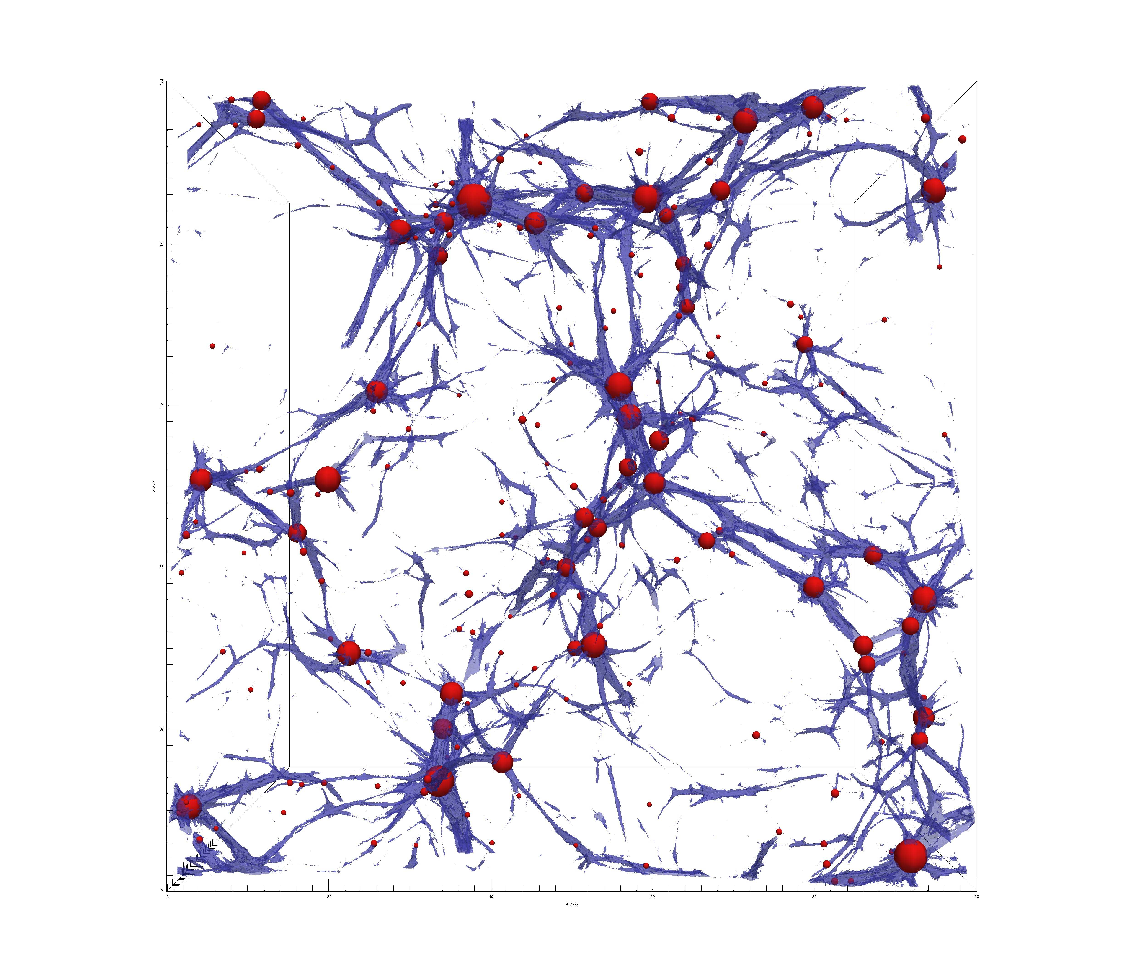
\includegraphics[width=18.5cm]{Chapter3/Source_v2/fig1.pdf} 
\caption{The cosmic web structure in a slice of  $30 h^{-1} \text{Mpc} \times 100 h^{-1} \text{Mpc} \times 100 h^{-1} \text{Mpc}$ in a simulation box of size $100 h^{-1}$ Mpc and $128^3$ particles. Regions with 17 or more streams (blue) form a filamentary structure. The haloes determined by FOF (red) are predominantly embedded in the intersections of the filaments.}
\label{fig:1full}
\end{figure}

The filamentary structure of regions with 17 or more streams (denoted as 17+ ) is shown for a slice of simulation box of size $100 h^{-1}$  Mpc and $128^3$  particles in Figure \ref{fig:1full}. It has to be noted that all the regions with 17+ streams are regions with 3+ streams. Thus, the filaments are just interior
parts  of walls with higher $n_{str}$. These are visually observed mostly at the intersections of walls. Further, at the intersections of multiple filaments, there are regions with locally maximum number of streams, signifying the most dense regions in the simulations i.e. the dark matter haloes as Figure \ref{fig:4view}
illustrates.
By superimposing the positions from the FOF-halo catalog, it is visually confirmed that the FOF haloes reasonably coincide with these high-streaming intersections, as Figure \ref{fig:1full} illustrates.

\subsection{Volume and mass fractions}

The single-stream flow, which corresponds to the void, occupies majority of volume of the simulation box (Figure \ref{fig:1m_v_fr}). As mentioned in Section \ref{sec:global}, higher multi-streaming flow regions are nested inside the lower streaming regions. Thus the volume occupied by higher number of streams monotonically decreases with the number of streams. This relation is approximately found to be a power law. For the box of size $L =100 ~h^{-1}$ Mpc and $N = 128^3$ particles ($L/N = 0.78 ~h^{-1}$ Mpc), the volume fraction corresponding to each value of number of streams, $ f_{vol}(n_{str})$ in the multi-stream field calculated with refinement factor of 8 (i.e. the multi-stream field
was computed on 1024$^3$ grid as described in \cite{Shandarin2012}) is 
\begin{equation}
\label{eq:fr_vol}
f_{vol}(n_{str}) =  0.69 n_{str}^{-2.5}
\end{equation}


This is a good fit for the range of number of streams $n_{str} \ge 5 $. In multi-stream field for the simulation box mentioned above, about 93$\%$ of the volume is occupied by 1-stream. With an increase in $n_{str}$, the corresponding volume fraction reduces. Physically, however, the number of streams reflect the advancement of non-linearity. Hence the higher $n_{str}$ regions are typically regions with higher densities. In effect, the mass fraction can also be approximated by a decreasing power law function of $n_{str}$,  
\begin{equation}
\label{eq:fr_mass}
f_{mass}(n_{str}) = 0.61 n_{str}^{-1.3}
\end{equation}
This is also a good fit for the range of number of streams $n_{str} \ge 5 $. For the same range of number of streams, the mean density in the regions with particular number of streams, given by the  ratio of corresponding mass and volume fractions, increases as expected.
%Note that, this estimator of mean density is different from the density of streams, which can be directly calculated from the volume and number of intersecting tetrahedra in the phase-space tessellation field.  
\begin{equation}
\label{eq:den}
{\bar{\rho}(n_{str}) \over \langle{\rho}\rangle} = 0.89  n_{str}^{1.2} ,
\end{equation}
where $\langle\rho\rangle$ is the mean density of the universe.
This also quantifies our previous claim that very high multi-streams correspond to the most dense areas in the Universe, i.e. the condensed haloes. The common over-density threshold of 200 using virial equilibrium corresponds to roughly 90 streams in  Figures ~\ref{fig:1m_v_fr} and Eq. ~\ref{eq:den}.

\begin{figure}
\begin{minipage}[t]{.99\linewidth}
  \centering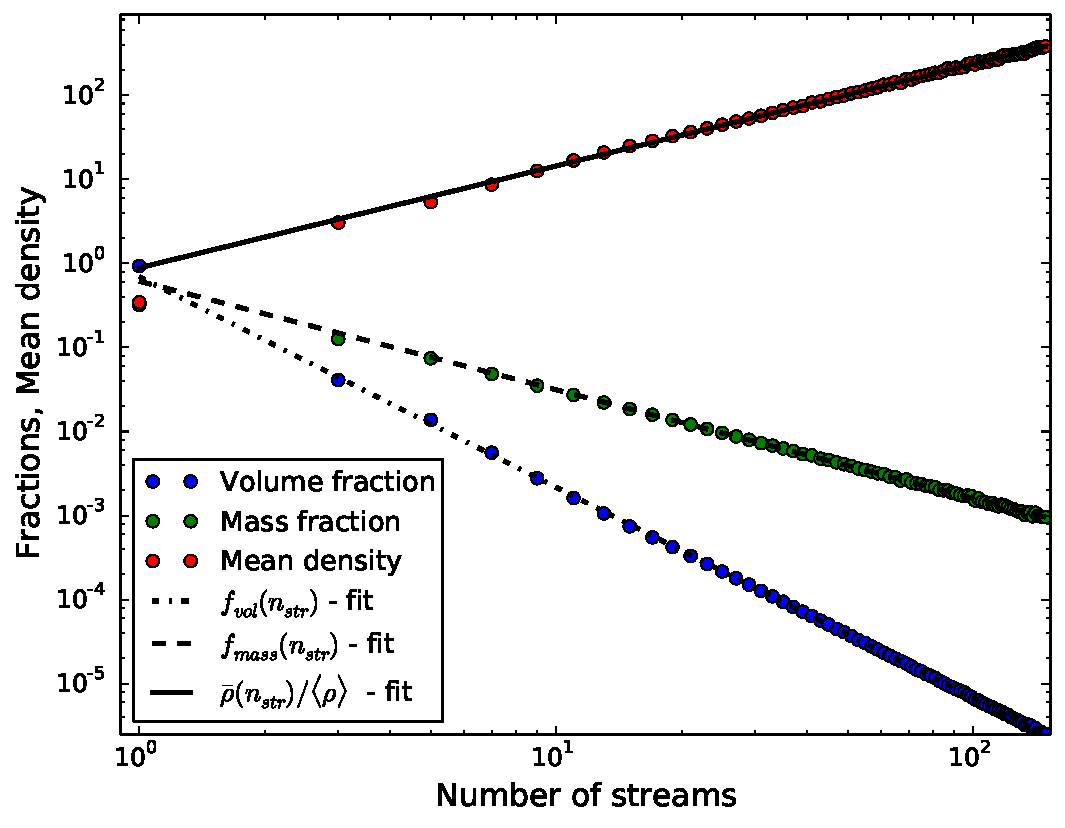
\includegraphics[width=10.cm]{Chapter3/Source_v2/fig2} 
\end{minipage}\hfill
\caption{Volume and mass fraction of each stream, mean density of each stream in a box of size 100 $h^{-1}$ Mpc and  $128^3$ particles. Exact values of fractions, density and their curve fit for the range $n_{str} \ge 5 $ from Eq.~\ref{eq:fr_vol}, Eq.~\ref{eq:fr_mass} and Eq.~\ref{eq:den} are shown. Multi-streams are calculated with refinement factor of 8. The void ($n_{str} = 1$) occupies 93$\%$ of the volume and 55$\%$ of the mass. }
\label{fig:1m_v_fr}
\end{figure}

Comparing the volume fractions of various simulation boxes in Figure ~\ref{fig:1Vfr_all} and corresponding power law dependences in Table ~\ref{tab:Compare_Slopes} (also, specifically for the volume fraction of voids in Table ~\ref{tab:Compare_LN}), we find that the profile is similar for boxes with
same inter-particle resolution; i.e., equal box length to grid size ratio( For e.g., $L/N = 0.78$ $h^{-1}$ Mpc for the simulation box of 100 $h^{-1}$ Mpc - $128^3$ particles and 200 $h^{-1}$ Mpc - $256^{3}$ particles). The box with minimum inter-particle resolution in the data, hence the best raw resolution ( $L/N = 0.19$ $h^{-1}$ Mpc for 100 $h^{-1}$ Mpc, $512^3$ particles), has higher volume fraction for each multi-stream compared to lower resolution boxes. Additionally, it has a more non-linear stage advanced over time resulting from the initial small scale perturbations. The advancement of  non-linearity manifests itself in higher number of streams. Box with the least raw inter-particle resolution ($L/N = 1.56 $  $h^{-1}$ Mpc for 200 $h^{-1}$ Mpc, $128^3$ particles), occupies lower volumes than other boxes for each $n_{str}$. It is also prone to noise at very high streaming regions.

One of the advantages of using tessellation is the freedom to compute densities at very high resolutions (\cite{Abel2012}, \cite{Shandarin2012}). We remind that the parameter `refinement factor' denotes the ratio of separation of the particles to the separation distance of points in the diagnostic grid as defined in Sec. 3. High refinement factors are extensively used in understanding stream behavior not only in the halo environment, but inside the halo too (Section ~\ref{sec:local}). The volume fractions of resulting number of streams are
%normalized by multi-stream field resolution (i.e. dividing by the cube of refinement factor) are %
similar for all refinement factors as
shown in bottom of the Figure ~\ref{fig:1Vfr_all} and in Table ~\ref{tab:Compare_ref}. % Hence our triangulation algorithm is universal in the sense that it is independent of the refinement factors used in tessellating the box.   
Multi-stream fields calculated on low refinement factors are more noisy at high number of streams.

With same refinement factors, the mass fractions exhibit similar pattern for same $L/N$ as well (Figure ~\ref{fig:Mfr_all}). The simulation box with highest inter-particle distance (thus least mass resolution) has more mass particles in single streaming region, as tabulated in Table~\ref{tab:Compare_LN}, but decreases steeply thereafter (Table ~\ref{tab:Compare_Slopes}). Unlike the volume fraction, the behavior of mass fraction has a systematic variation across different refinement factors. The mass fractions given in Table ~\ref{tab:Compare_ref} show that the single-streaming regions in the multi-stream fields with refinement factors 1 and 2 have higher mass fraction than in the fields with refinement factor of 8. Decreasing the resolution from refinement factor of 8 to 1 effectively introduces smoothing of the structure. This results in growth of mass fraction in voids ($n_{str} = 1$) and decreasing it in the web ($n_{str} > 1$). The multi-stream field is more robust as one can see in Figure ~\ref{fig:1Vfr_all}. and \ref{fig:Mfr_all}. In addition, the less refined multi-stream grids are prone to noise at high $n_{str}$ as usual.
\begin{figure}
\begin{minipage}[t]{.99\linewidth}
 \centering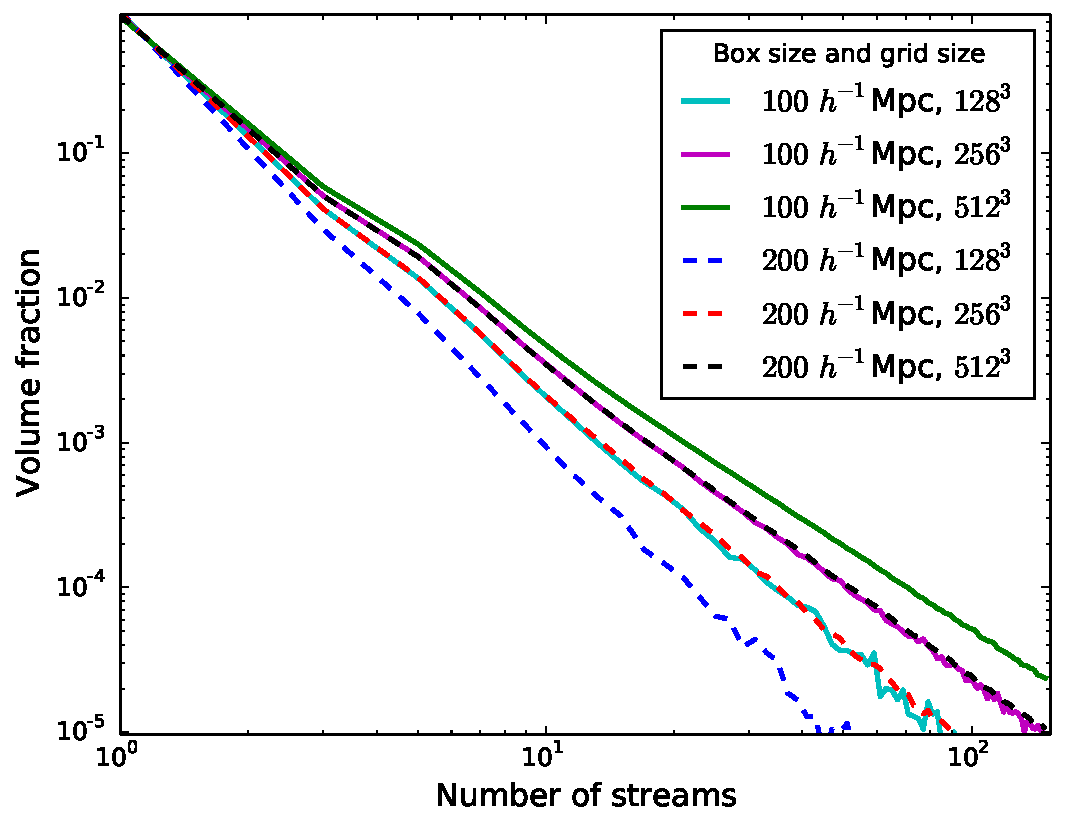
\includegraphics[width=10.cm]{Chapter3/Source_v2/fig3a} 
  \centering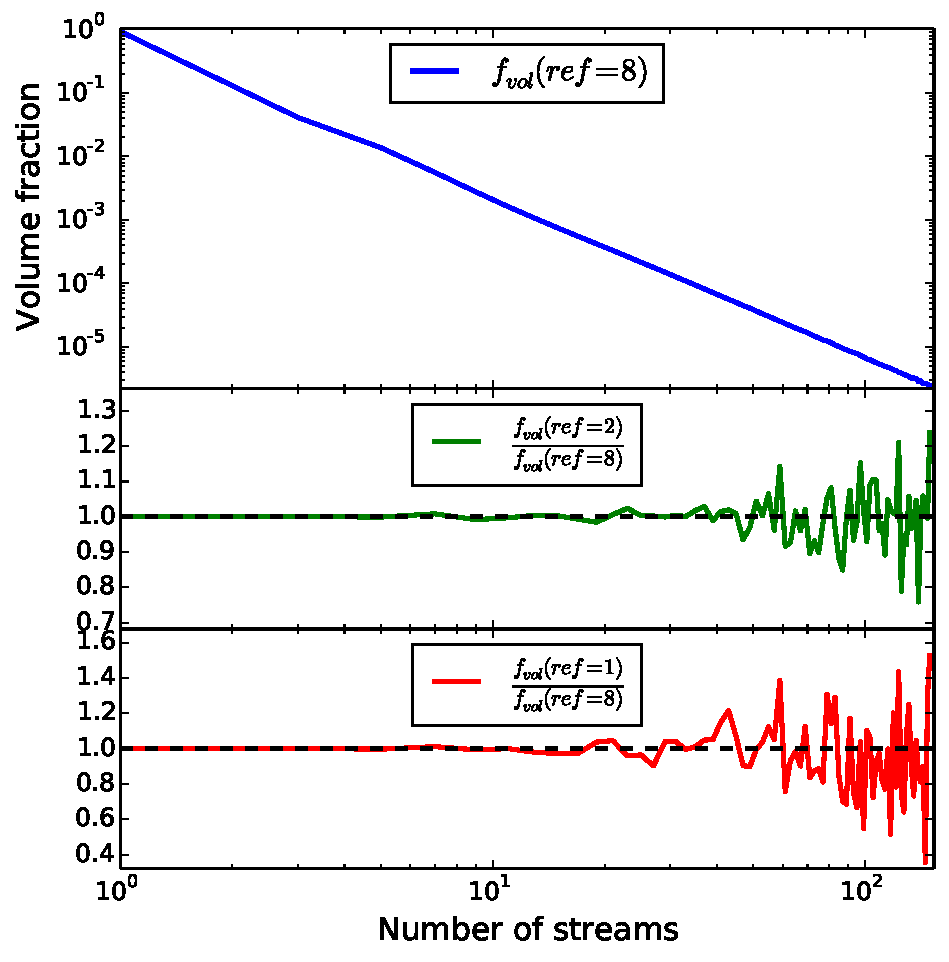
\includegraphics[width=10.cm]{Chapter3/Source_v2/fig3b}
\end{minipage}\hfill
\caption{Top: Volume fraction distribution of streams in 6 simulation boxes of size 100 $h^{-1}$ Mpc, 200 $h^{-1}$ Mpc 
and $128^{3}$, $256^{3}$, $512^{3}$ grids (with refinement factor of 1). Volume fractions are similar for simulation boxes with same inter-particle resolution. Slopes of the curve fits are shown in Table ~\ref{tab:Compare_Slopes}. Bottom: Volume fraction distribution for different refinement factors for 100 $h^{-1}$ Mpc, $128^{3}$ box. A considerably smoother volume fraction distribution is obtained at high number of streams in multi-stream fields with high refinement factor. }
\label{fig:1Vfr_all}
\end{figure}

\begin{figure}
\begin{minipage}[t]{.99\linewidth}

  \centering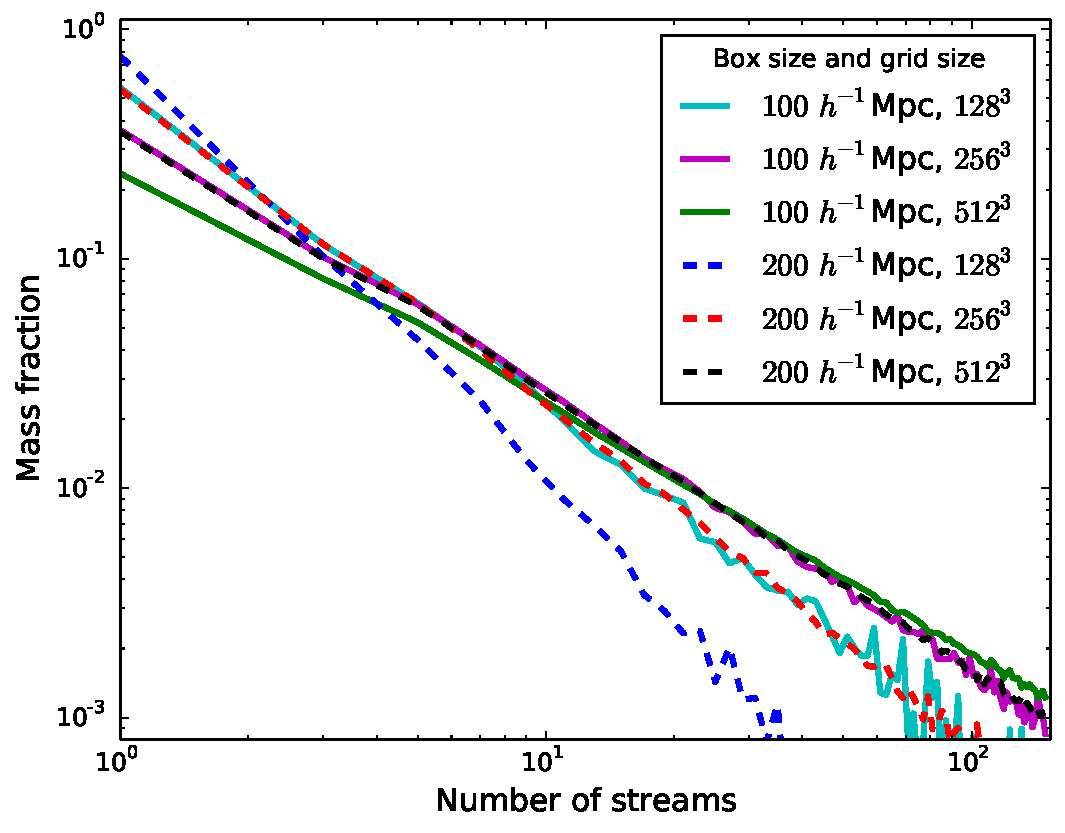
\includegraphics[width=10.cm]{Chapter3/Source_v2/fig4a} 
  \centering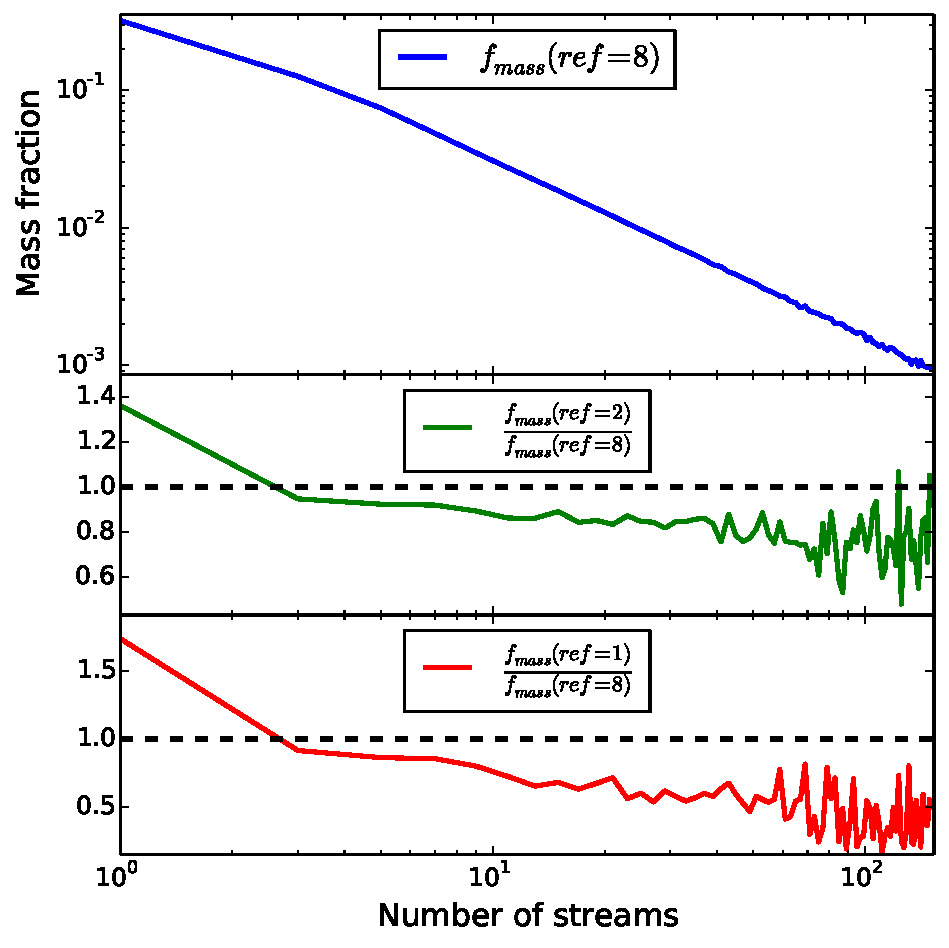
\includegraphics[width=10.cm]{Chapter3/Source_v2/fig4b}
\end{minipage}\hfill
\caption{Top: Mass fraction distribution of streams in 6 simulation boxes of size 100 $h^{-1}$ Mpc, 200 $h^{-1}$ Mpc 
and $128^{3}$, $256^{3}$, $512^{3}$ grids ( with refinement factor of 1). Mass fractions are similar for simulation boxes with same inter-particle resolution. Slopes of the curve fits are shown in Table ~\ref{tab:Compare_Slopes}. Bottom: Mass fraction distribution for different refinement factors for 100 $h^{-1}$ Mpc, $128^{3}$ box. Single-streaming void regions have more fraction of mass particles in multi-stream fields calculated at low refinement factors of 1 and 2. This effect is minimized when calculation is done at better refinement. In addition, mass fraction distribution is less noisy.}
\label{fig:Mfr_all}
\end{figure}

\begin{table}
\centering
  \caption{Comparison of the approximate power law dependences of curve fits in Figure \ref{fig:1Vfr_all} and Figure \ref{fig:Mfr_all}. Power law relations for volume fraction $f_{vol}(n_{str})$ and mass fractions $f_{mass} (n_{str}) $ as a function of number of streams at $n_{str} \geq 5$ are shown (amplitudes are not shown). The boxes of size 100 $h^{-1}$ Mpc on  $128^{3}$ grids and, 200 $h^{-1}$ Mpc on  $256^{3}$ grids have same  $L/N = 0.78 h^{-1}$ Mpc. Similarly, $L/N = 0.39 h^{-1}$ Mpc for boxes of size 100 $h^{-1}$ Mpc on  $256^{3}$ grids and, 200 $h^{-1}$ Mpc on  $512^{3}$ grids.}
\begin{tabular}{|l|r|r|r|r|}
\hline
%\multicolumn{1}{|c|}{} & \multicolumn{4}{l|}{Multi-stream analysis (This work)} & \multicolumn{4}{c|}{ORIGAMI \citep{Falck_Neyrinck:14}}    \\ \hline
$L/N$                & $0.19$ & $0.39$& $0.78$ & $1.56$  \\ \hline
$f_{vol} (n_{str}) $ Vs. $n_{str}$                 & $-2.1$   & $-2.3$    & $-2.5$      & $-2.9$  \\ \hline
$f_{mass} (n_{str}) $   Vs. $n_{str}$            & $-1.1$   & $-1.2$   & $-1.4$       & $-2.0$     \\ \hline
\end{tabular}
 \label{tab:Compare_Slopes}
\end{table}



 \begin{table}
 \centering
  \caption{Comparison of the volume and mass fractions of the void ($n_{str} = 1$) regions of the cosmic web for various simulation boxes at refinement factor of 1. Mean density is the ratio of mass fraction to the volume fraction. It is given in units of the mean density of the universe. The boxes of size 100 $h^{-1}$ Mpc on  $128^{3}$ grids and, 200 $h^{-1}$ Mpc on  $256^{3}$ grids have same  $L/N = 0.78 h^{-1}$ Mpc. Similarly, $L/N = 0.39 h^{-1}$ Mpc for boxes of size 100 $h^{-1}$ Mpc on  $256^{3}$ grids and, 200 $h^{-1}$ Mpc on  $512^{3}$ grids.}
\begin{tabular}{|l|r|r|r|r|}
\hline
%\multicolumn{1}{|c|}{} & \multicolumn{4}{l|}{Multi-stream analysis (This work)} & \multicolumn{4}{c|}{ORIGAMI \citep{Falck_Neyrinck:14}}    \\ \hline
$L/N$                & $0.19$ & $0.39$& $0.78$ & $1.56$  \\ \hline
Volume Fraction (\%)                 & $88$   & $90$    & $93$      & $96$  \\ \hline
Mass Fraction   (\%)               & $24$   & $36$   & $55$       & $77$     \\ \hline
Mean density                    & $0.27$ & $0.40$    & $0.59$        & $0.80$   \\ \hline
\end{tabular}
 \label{tab:Compare_LN}
\end{table}


 \begin{table}
 \centering
  \caption{Comparison of the volume and mass fractions of the void ($n_{str} = 1$) regions of the cosmic web for a simulation box at different refinement factors. Mean density is the ratio of mass fraction to the volume fraction. All the multi-streams for simulation box of length 100 $h^{-1}$ Mpc on raw resolution of $128^{3}$ grids ($ L/N = 0.78 h^{-1}$) }
\begin{tabular}{|l|r|r|r|}
\hline
%\multicolumn{1}{|c|}{} & \multicolumn{4}{l|}{Multi-stream analysis (This work)} & \multicolumn{4}{c|}{ORIGAMI \citep{Falck_Neyrinck:14}}    \\ \hline
Refinement factor               & $1$ & $2$& $8$   \\ \hline
Volume Fraction (\%)                 & $93$   & $93$    & $93$       \\ \hline
Mass Fraction   (\%)               & $55$   & $44$   & $32$           \\ \hline
Mean density                    & $0.59$ & $0.47$    & $0.35$        \\ \hline
\end{tabular}

 \label{tab:Compare_ref}
\end{table}



\section{Stream environment around haloes}
\label{sec:local}

Multi-stream field can be easily computed for a small Eulerian box with higher refinement factor. This can be utilized to analyze the phase-space behavior inside and around haloes. In this section, 
we have used the halo coordinates identified by the FOF method, and selected Eulerian boxes around it. A reasonable  correspondence between FOF halo centers and local maxima of multi-stream field is visually examined in Figure \ref{fig:1full}. 

Since each multi-stream region is surrounded by lower number of streams, the walls sandwich filaments within themselves (Figure \ref{fig:4view}). The filaments are embedded with haloes at various intersections. These high-streaming haloes are completely covered by relatively low-stream filaments and hence surrounded by walls too. This result differs considerably from the several void finder methods, which find existence of haloes within  void regions (See \citealt{Colberg2008} and references therein). By our classification, we distinguish configuration space of the simulation box as void and non-void or web regions. Further, we have made an attempt to classify the web into walls, filaments and haloes based on multi-stream thresholds. This classification based on number of stream threshold provides only a very crude description of visual impression from the richness, complexity and fundamentally multi-scale character of the web. The heuristic numbers we use in this chapter are by no means universal, but may provide limited use in the discussion of these particular simulations.

\begin{figure}
\centering
\begin{minipage}[c]{.45\linewidth}
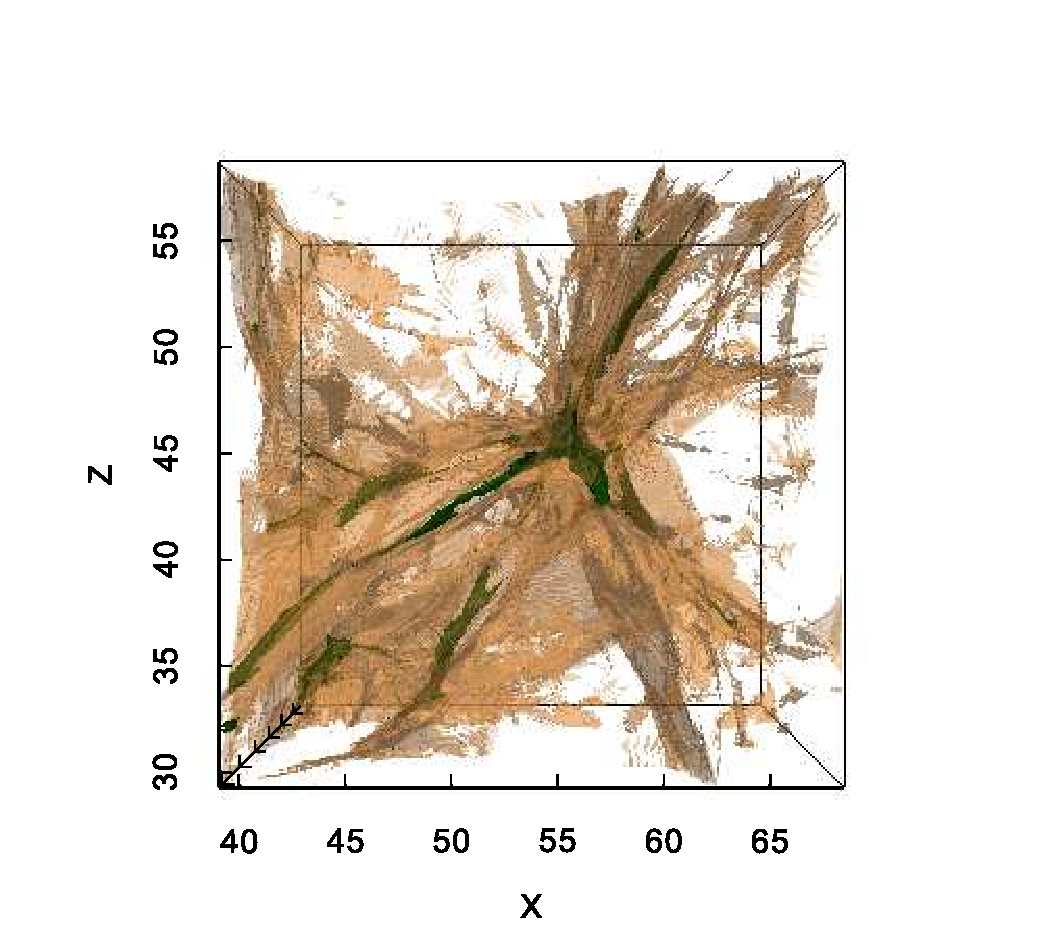
\includegraphics[width=9.cm]{Chapter3/Source_v2/fig5a} 
\end{minipage}
\begin{minipage}[c]{0.45\linewidth}
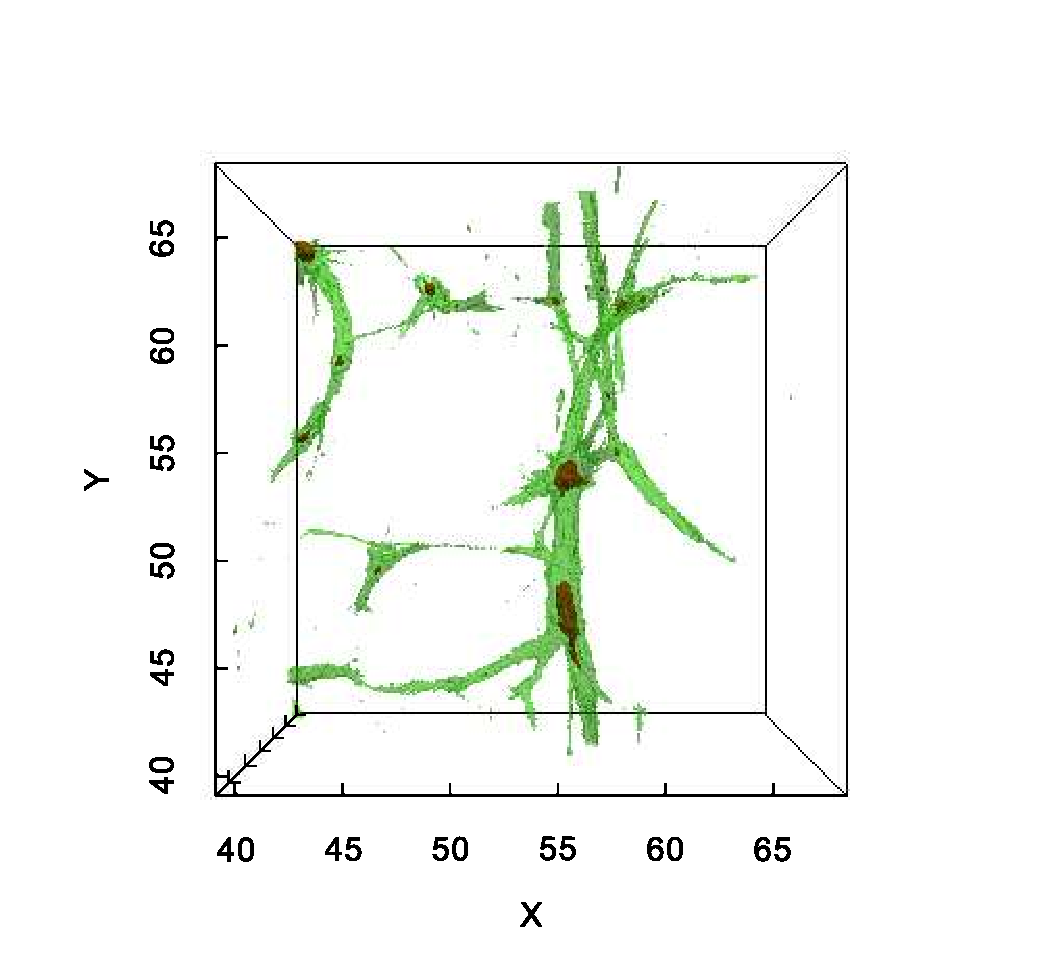
\includegraphics[width=9.cm]{Chapter3/Source_v2/fig5b} 
\end{minipage} 
\begin{minipage}[c]{0.45\linewidth}
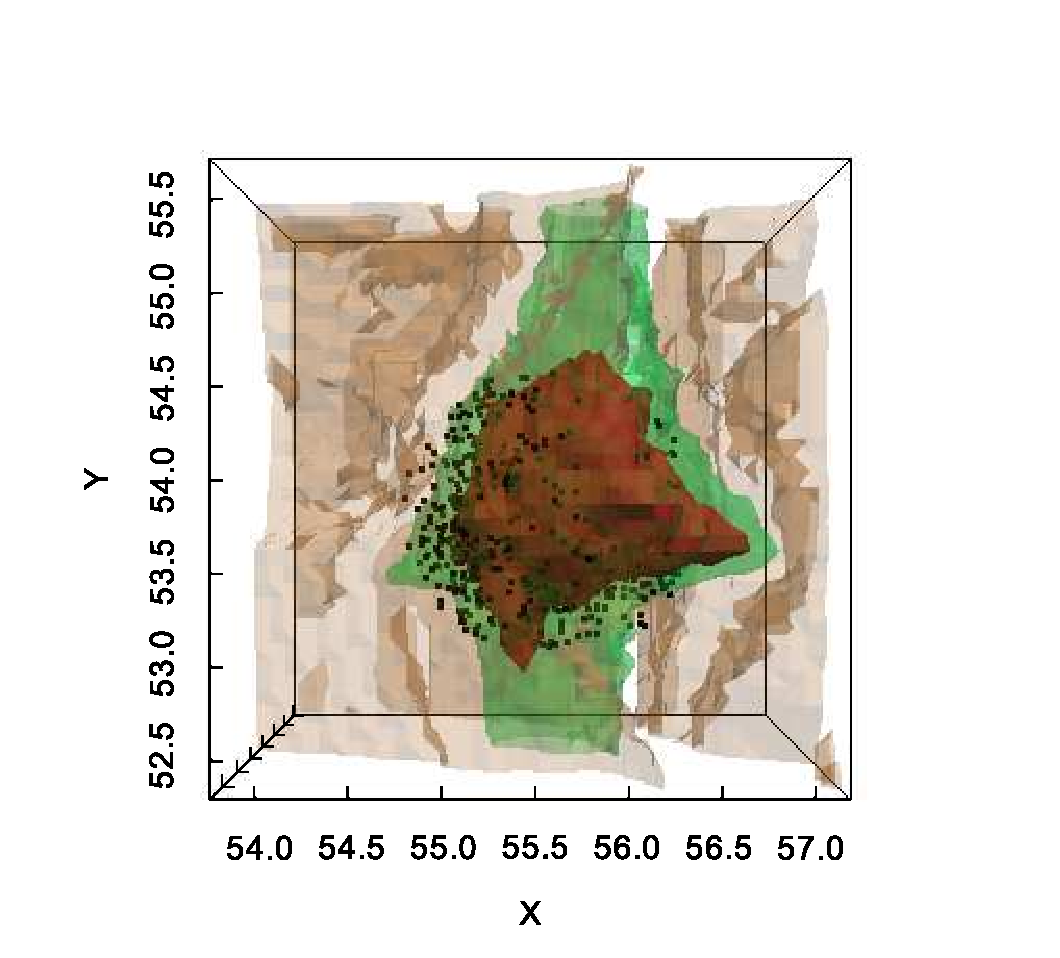
\includegraphics[width=9.cm]{Chapter3/Source_v2/fig5c} 
\end{minipage}
\begin{minipage}[c]{0.45\linewidth}
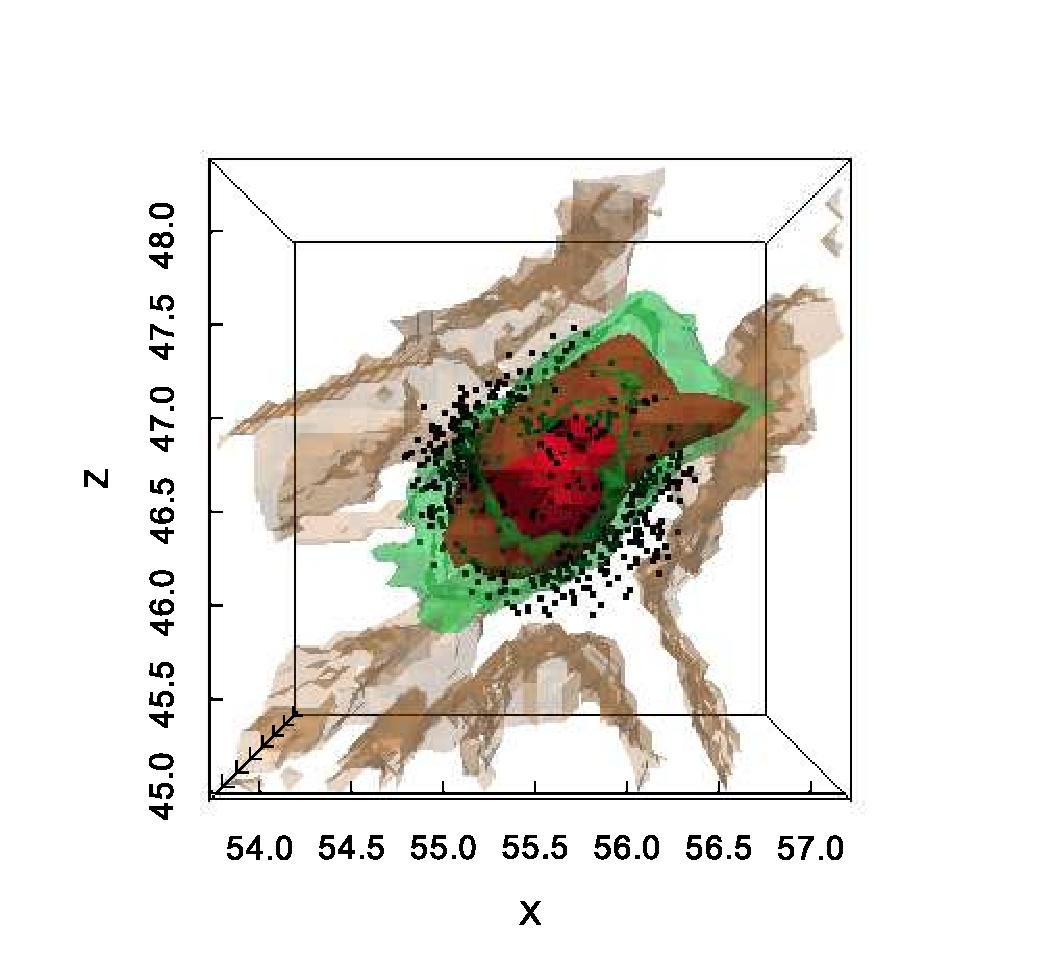
\includegraphics[width=9.cm]{Chapter3/Source_v2/fig5d} 
\end{minipage} 

\caption{Multi-stream flow regions in a small box of the simulation. Top left: regions with more than 3-stream flow are identified as walls (brown). Intersection of multiple walls have higher $n_{str}$ regions (green, 17+ streams). Single-streaming voids (white) occupy large volume and are very close to the filaments in some directions. Top right: 17+ streams (green) form filamentary structures with nodes at the intersections (red, 90+ streams)
Bottom left and right:  Closer look at the highly non-linear region reveals that a filament is sandwiched between the walls (brown). The 90+ stream region (red) forms a compact structure and is entirely contained within the filament. The black dots show the particles around the FOF halo within linking length of 0.2.}
\label{fig:4view}
\end{figure}

Visual inspection of Figure \ref{fig:4view} reveals that the multi-stream environment of a halo is a highly intricate. Though the haloes are surrounded by filaments and walls, it can be surprisingly close to the voids in particular directions. Filaments 
defined by the multi-steam field are  quite elongated, but the cross-sections are not circular or elliptical, and moreover, they branch-out and intersect at several regions. Finally, the  haloes defined by contours of the multi-steam field look neither spherical nor ellipsoidal. 
We use a simple geometrical technique of projecting the number of streams onto a diagnostic spherical surface around 
a haloes to visualize and quantify their environments.  


\subsection{Technique}

Motivated by the complicated morphology of multi-stream field around a dark matter halo, we devised an empirical 
statistical tool to quantify the multi-stream environment of the FOF haloes. The method is geometrical and non-local.
We  randomly select a large number of points on a diagnostic spherical surface centered at the FOF center of the halo 
and compute the number of streams  at these points. By increasing the radius of the sphere from inside of the halo to several times the halo radii, we estimate  the fractions of the area on the diagnostic spherical surface occupied by the regions with different numbers of streams:
3+, 5+, ..., where $n+$ corresponds to $n$ or higher number of streams. 

 
The geometry of a filament can be crudely approximated by a cylinder and that of a wall by a sheet with a small constant thickness 'd'. Upon intersecting with the spherical surface, these geometries occupy certain cross-sectional area, $Area_{c/s}$, on the sphere (See Figure ~\ref{fig:model}). The ratio of this area to the surface area of the sphere  is given by \autoref{eq:model} and \autoref{eq:model2},
% --- COMMENTED -- some thesis latex issue with sub-equations -- gonna write separately. 
% \begin{subequations} \label{eq:model}
% \begin{align}
%  f_{wall} (r) &= \frac{Area_{c/s}}{4\upi r^2} = \frac{2\upi r d}{4\upi r^2} \propto r^{-1} \\
%  f_{fil} (r) &= \frac{Area_{c/s}}{4\upi r^2} = \frac{\text{const.}}{4\upi r^2} \propto r^{-2}
% \end{align} 
% \end{subequations}



\begin{equation} \label{eq:model}
 %\begin{align}
  f_{wall} (r) = \frac{Area_{c/s}}{4\pi r^2} = \frac{2\pi r d}{4\pi r^2} \propto r^{-1} \\
 %\end{align} 
 \end{equation}

 
 
  \begin{equation} \label{eq:model2}
 %\begin{align}
 f_{fil} (r) = \frac{Area_{c/s}}{4\pi r^2} = \frac{\text{const.}}{4\pi r^2} \propto r^{-2}
 %\end{align} 
 \end{equation}

The fractions of points on the surface of the sphere by multiple number of intersecting sheet-like walls or cylindrical filaments also scale proportional to $ r^{-1}$ and $ r^{-2}$ respectively. 

\begin{figure}
\begin{minipage}[t]{.99\linewidth}
 \centering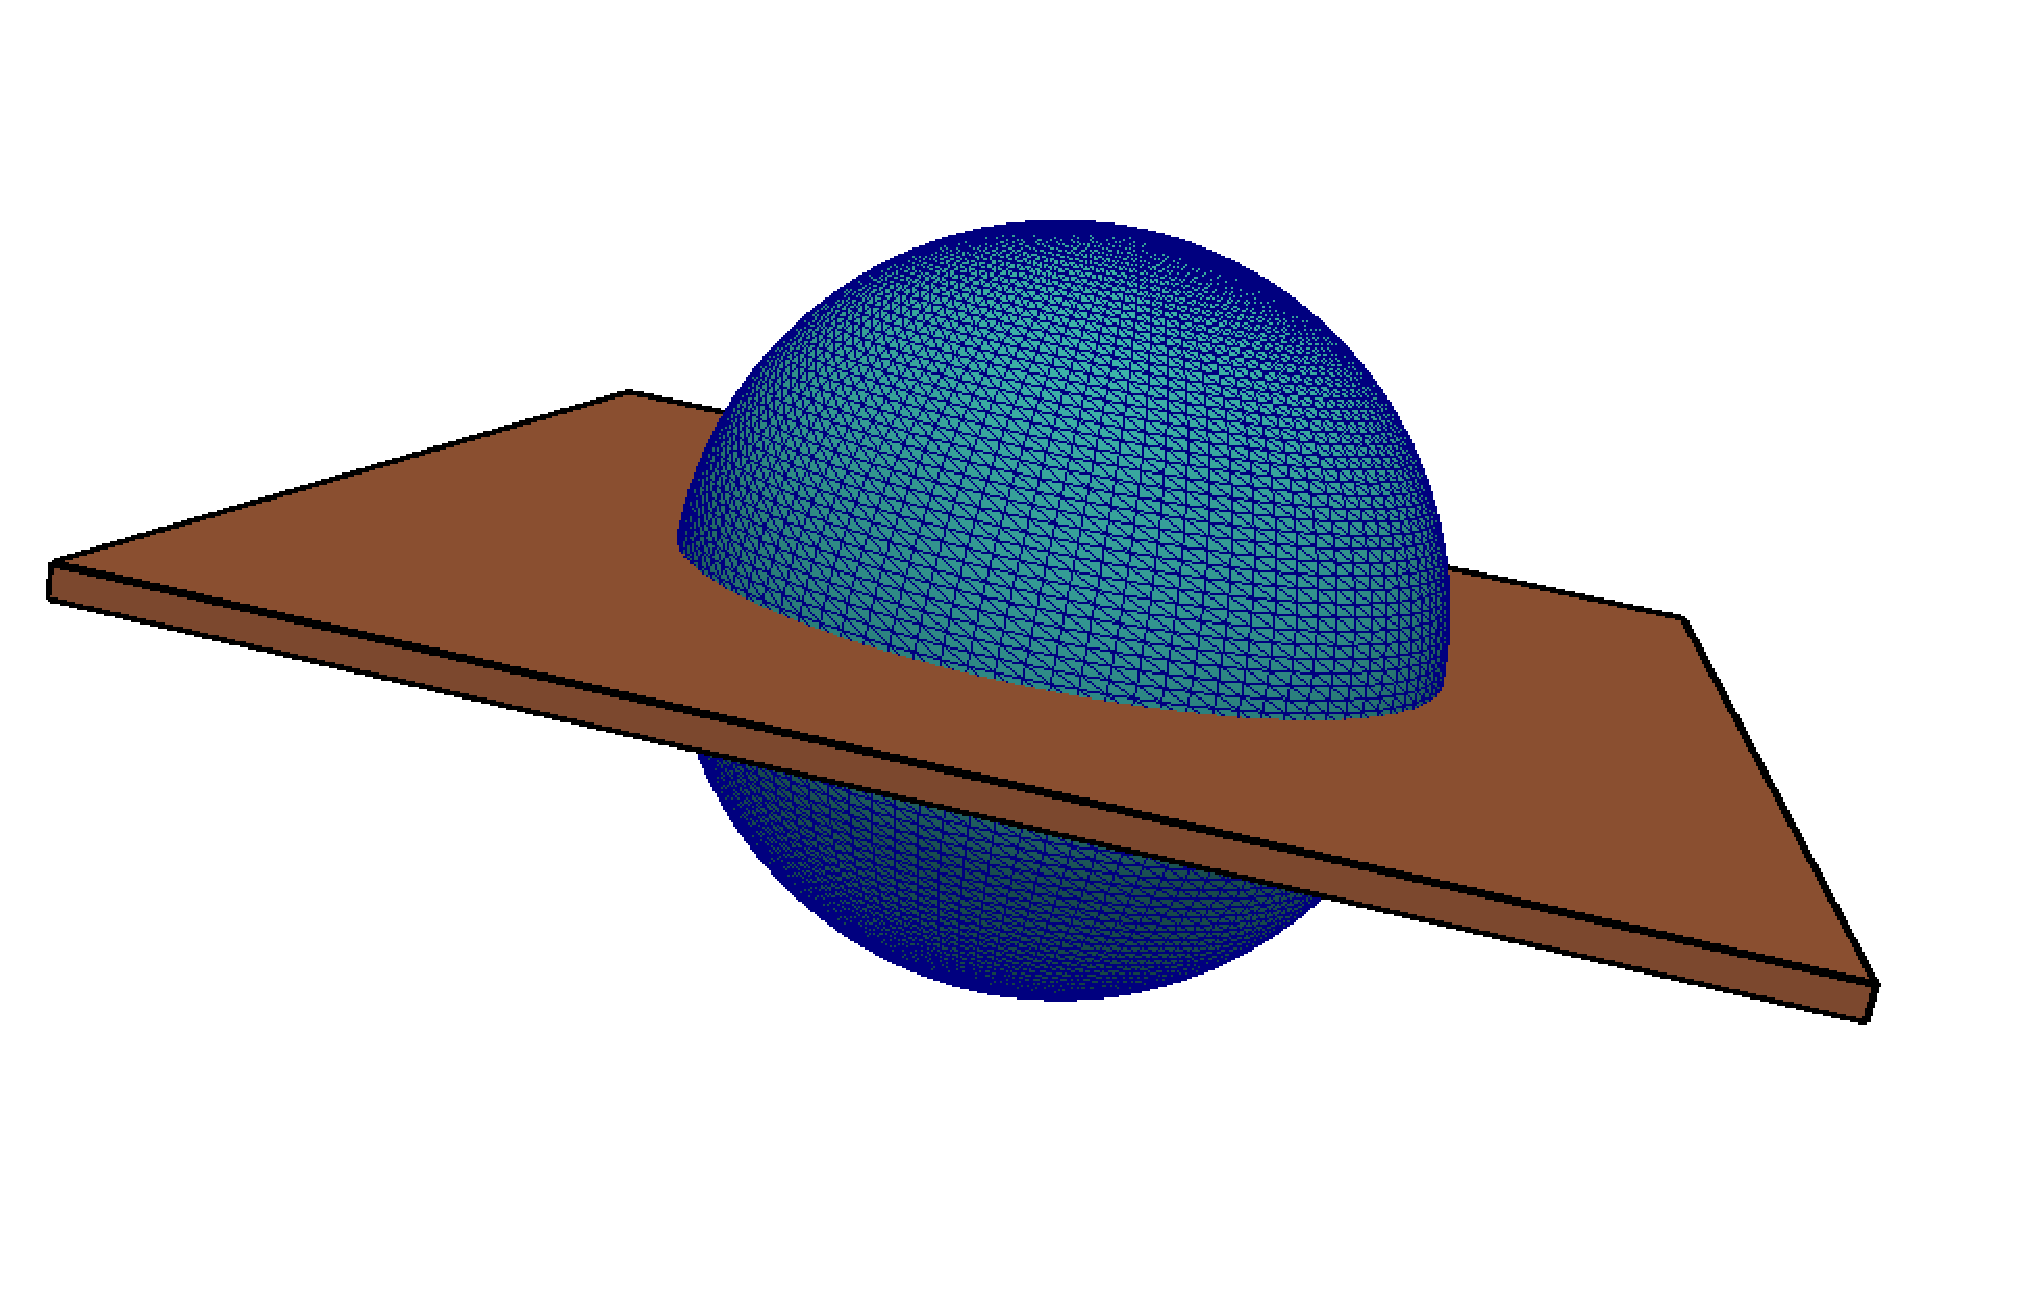
\includegraphics[width=10.cm]{Chapter3/Source_v2/fig6a} 
  \centering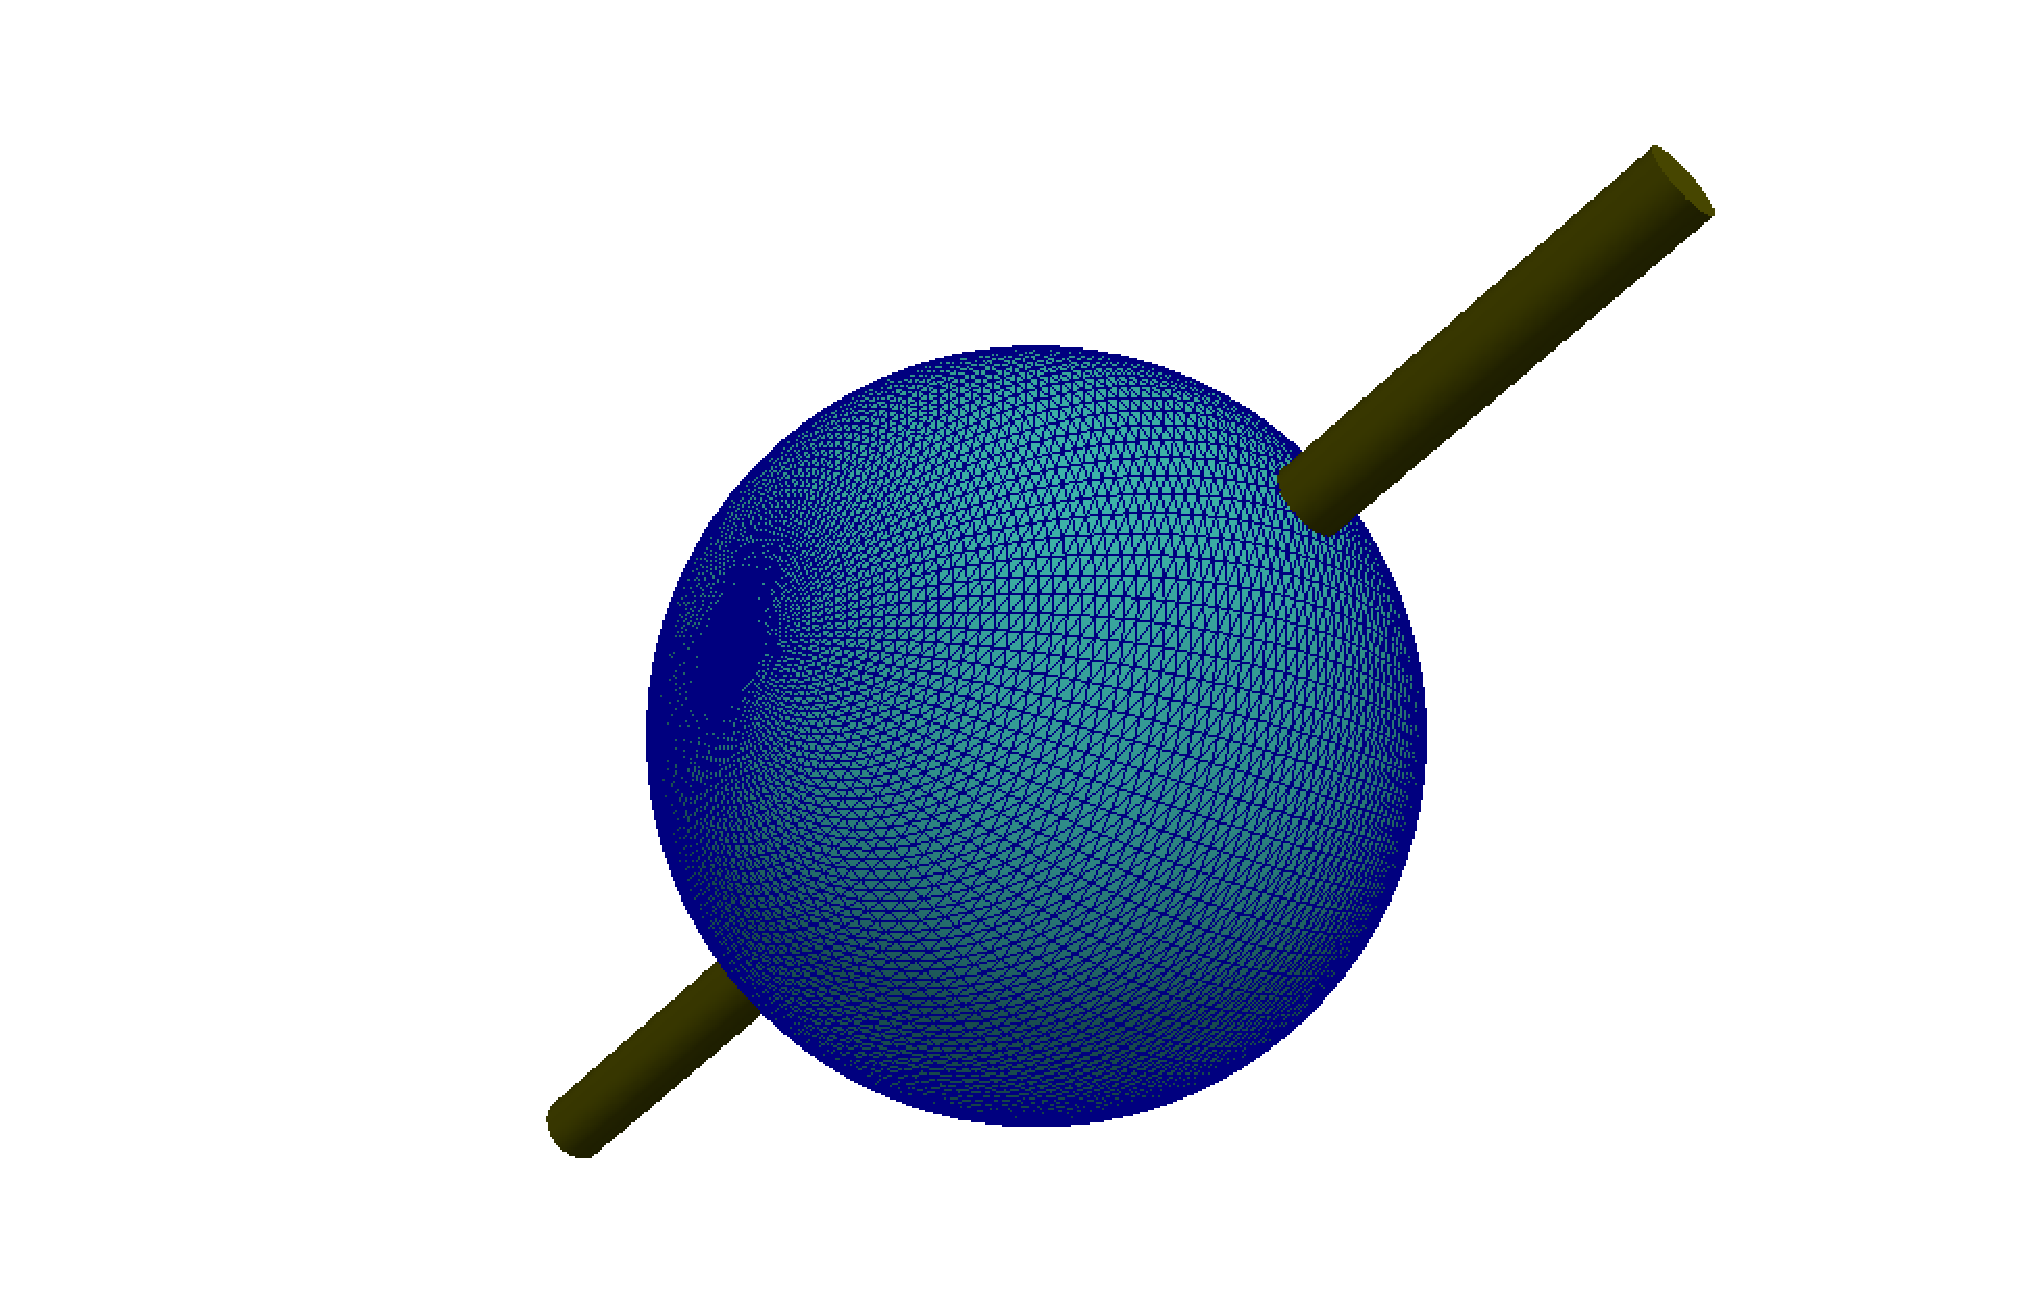
\includegraphics[width=10.cm]{Chapter3/Source_v2/fig6b}
\end{minipage}\hfill
\caption{Modeling a wall and a filament. A diagnostic spherical surface is intersected by a cylinder and plane.}
\label{fig:model}
\end{figure}


For the diagnostic spheres of different radii, the  scaling of multi-streams at the intersections is calculated. By checking the 
variation in the fraction of area occupied, we associate the number of streams with wall or halo. 

Each of the Mollweide projections in Figures ~\ref{fig:3} - ~\ref{fig:4322} shows projection of the multi-stream field on to the 
spherical surface, and provide useful insight into the multi-stream structure around a halo. %\citet{Rieder:2013} shows similar projections for %density of dark matter around haloes. 
In a Mollweide projections, each filament stemmed from the halo looks as a compact patch. If the physical area of the cross 
section of the filament remains approximately constant, then the size of the patch on the Mollweide projection would decrease with the increasing radius of the diagnostic sphere. The cross section of a wall with the diagnostic sphere has a well known
`S'-shape (similar to the ecliptic plane in the galactic coordinates) and the width decreases with the growth of the diagnostic sphere. Both patterns are clearly seen in  Figures ~\ref{fig:3} - ~\ref{fig:4322}.


\subsection{Voids, filaments and walls around haloes}

From the technique described  above, we arrive at quantitative thresholds for the different components of the web i.e., all regions where
$n_{str} \ge 3$. We stress that this method is only a practical tool in arriving at heuristic thresholds of cosmic web structures. The analysis done here are for the simulation box of 100 $h^{-1}$ Mpc, 128$^3$ particles, with refinement factor of 8.

%For the non-linear regions, the volume fraction of flows with 3 or higher streams is greatest. 
The scaling of fraction of points with 3+ streams is closest to $r^{-1}$, where $r$ is the radius of the diagnostic sphere around the halo (Figures ~\ref{fig:3} - ~\ref{fig:4322}; top figures). Since $r^{-1}$ variation is geometrically identical to that of a wall, it is identified as a flow region with 3+ stream flow. In this simulation the volume fraction of the web is dominated by 3-stream flows: $f_{vol}(3) \approx 0.04$ while
$\sum_5^{\infty} f_{vol}(n_{str}) \approx 0.02$.  

The deviation from the exact slope is expected, since assuming the filaments and walls as uniform cylinders 
and planes is rather crude. In the simulation, the filaments and walls have a far more complicated structure, where they branch out, and do not correspond to regular geometrical shapes. Detailed explanations for deviations are illustrated using Mollweide projections in the next section. 

Variation of multi-streams regions of 5+ to 17+ streams steadily changes from $r^{-1}$ to $r^{-2}$. This smooth transition implies that finding an exact cut-off of $n_{str}$ for  a filament is possible neither $n_{str}$ threshold nor by density. At 17+ stream regions scaling is closest to $r^{-2}$, the approximate filamentary geometry. In fact, $n_{str} = 19+$ regions also exhibit similar variation in spherical projections, but our choice of the threshold based on the lowest $n_{str}$ value that scales close to $r^{-2}$. Again, unlike the threshold for voids and walls, the threshold for filaments and haloes are not unambiguous. Our seemingly arbitrary choice of definition of filaments as regions with 17+ streams (in Section \ref{sec:global}, Figures \ref{fig:1full} and Figures \ref{fig:4view}) was motivated by this observation. 
Thus projections on a diagnostic sphere is a convenient tool for classifying regions in the simulation as belonging to void, wall, filament or a halo. 

\begin{figure}
\begin{minipage}[t]{.99\linewidth}
  \centering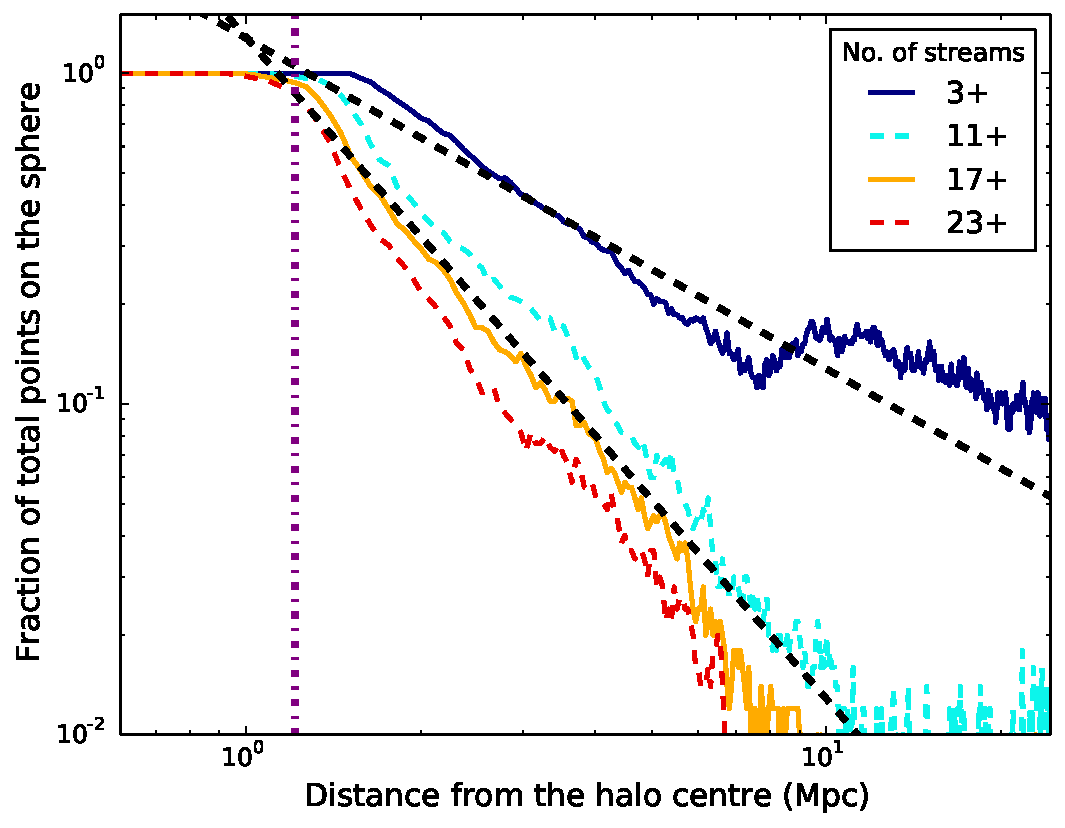
\includegraphics[width=10.cm]{Chapter3/Source_v2/fig7a}
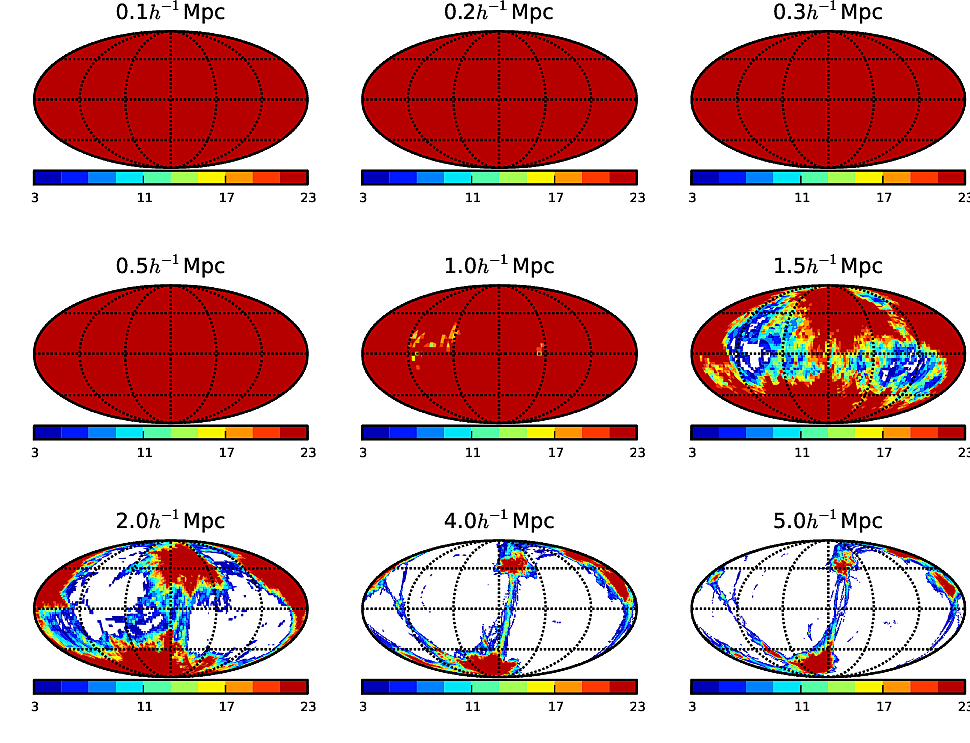
\includegraphics[width=10.cm]{Chapter3/Source_v2/fig7b} 
\end{minipage}\hfill
\caption{ Large halo of mass $3.7 \times 10^{14}M_{\odot} $  and FOF radius 1.2 $h^{-1}$ Mpc (dotted-violet line in the top figure). Top: Fractional distribution of streams on the surface of spheres of increasing radii. Dashed-black lines are for $r^{-1}$ and $r^{-2}$ scaling. 3+ streams are closest to $r^{-1}$ and 17+ scales close to $r^{-2}$. for higher thresholds, the fractional distribution departs smoothly from $r^{-2}$. Bottom: Mollweide projection of multi-streams on the surface of the sphere.}
\label{fig:3}
\end{figure}

\begin{figure}
\begin{minipage}[t]{.99\linewidth}
  \centering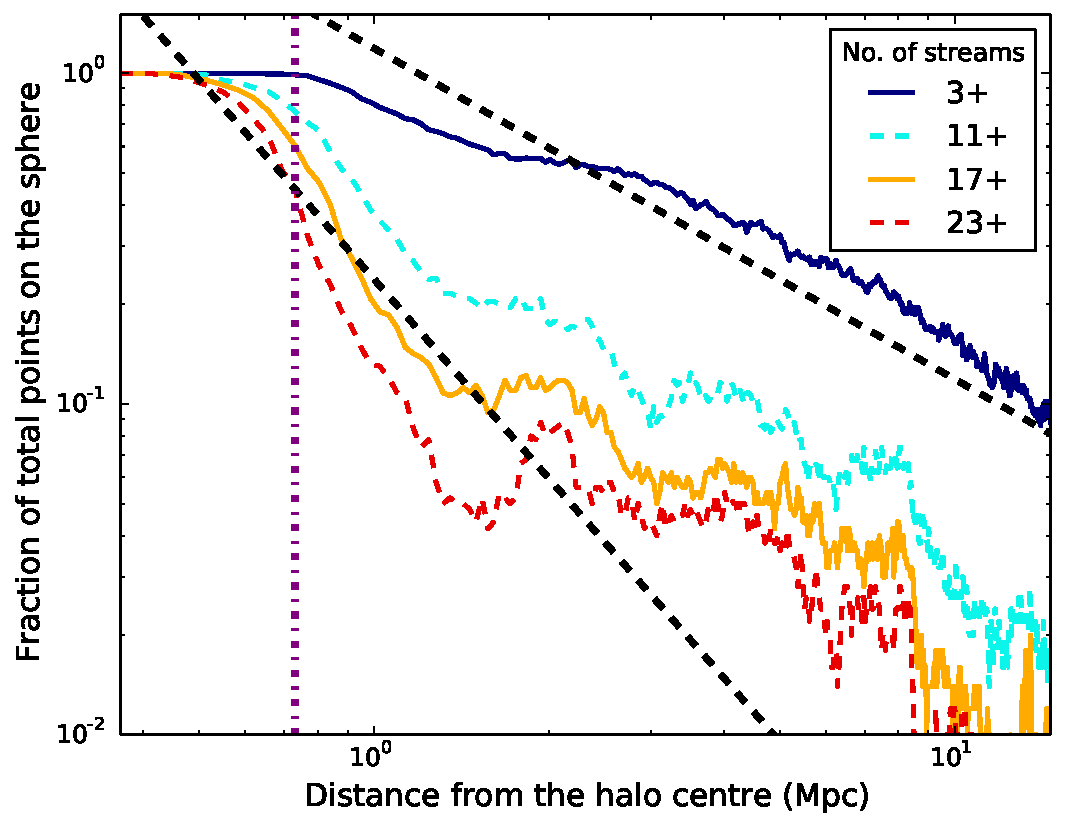
\includegraphics[width=10.cm]{Chapter3/Source_v2/fig8a}
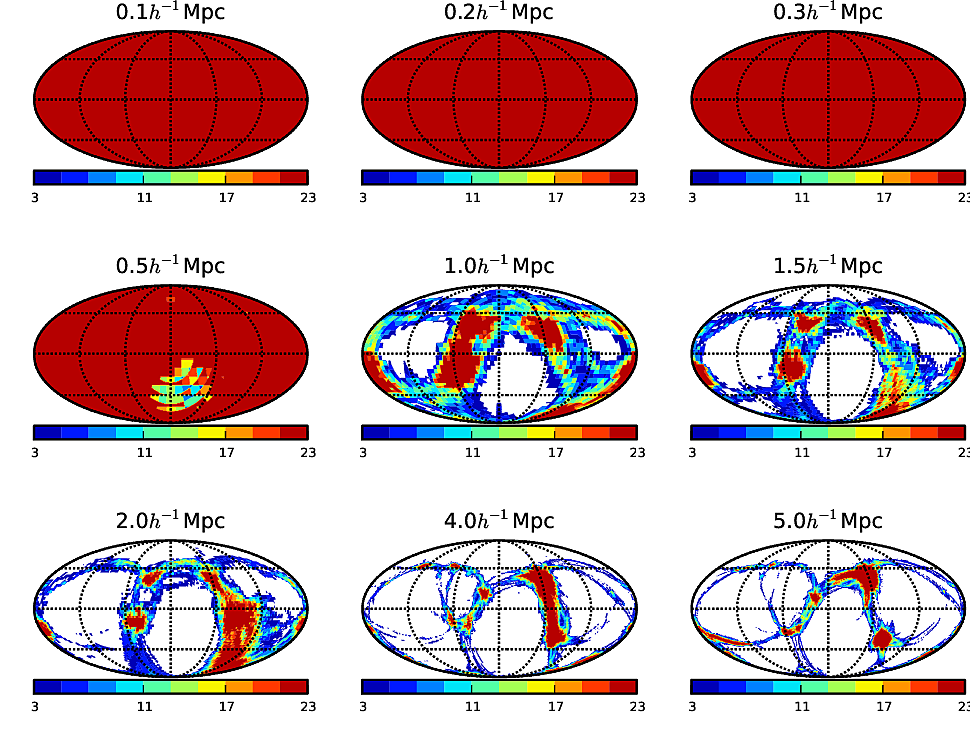
\includegraphics[width=10.cm]{Chapter3/Source_v2/fig8b} 
\end{minipage}\hfill
\caption{ Halo of mass $5.0 \times 10^{13} M_{\odot} $   and  FOF radius 0.7 $h^{-1}$ Mpc. Top: Fractional distribution of streams deviates from $r^{-1}$ and $r^{-2}$ scales
since the high stream filament passes along the surface of the sphere. Bottom: Filament passing through the surface is 
seen from 2 to 5 times the halo radius. }
\label{fig:79}
\end{figure}

\begin{figure}
\begin{minipage}[t]{.99\linewidth}
  \centering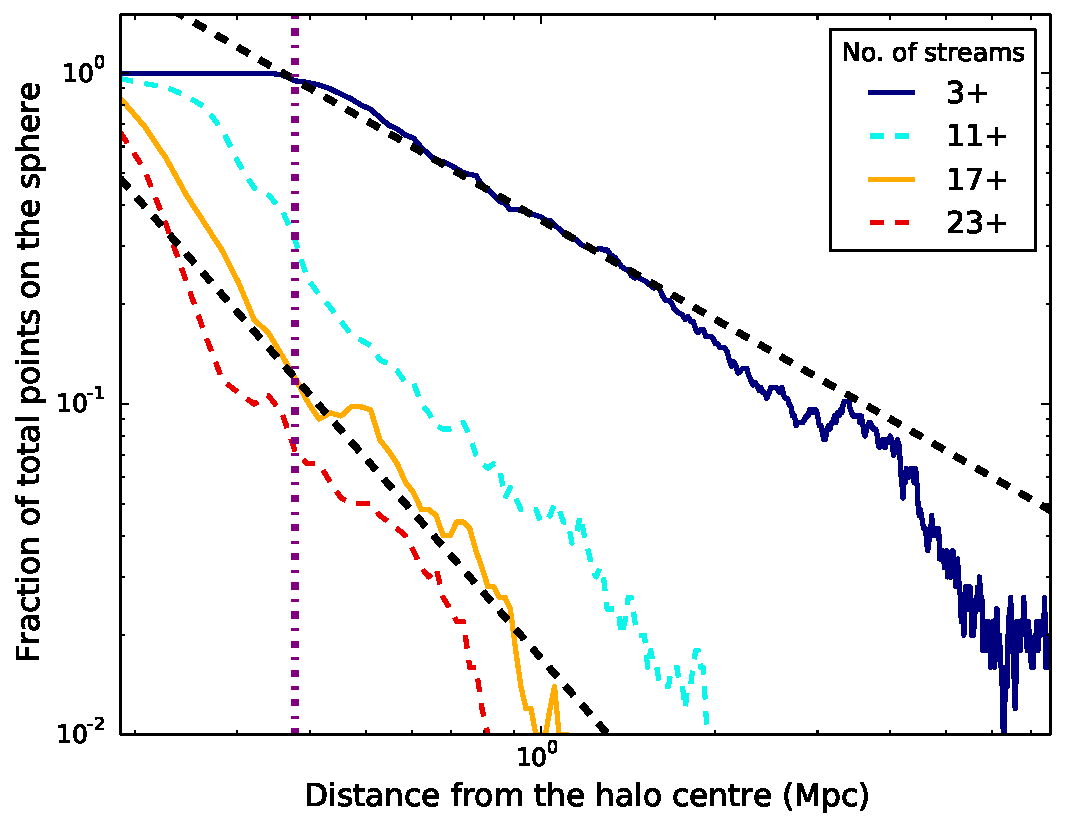
\includegraphics[width=10.cm]{Chapter3/Source_v2/fig9a}
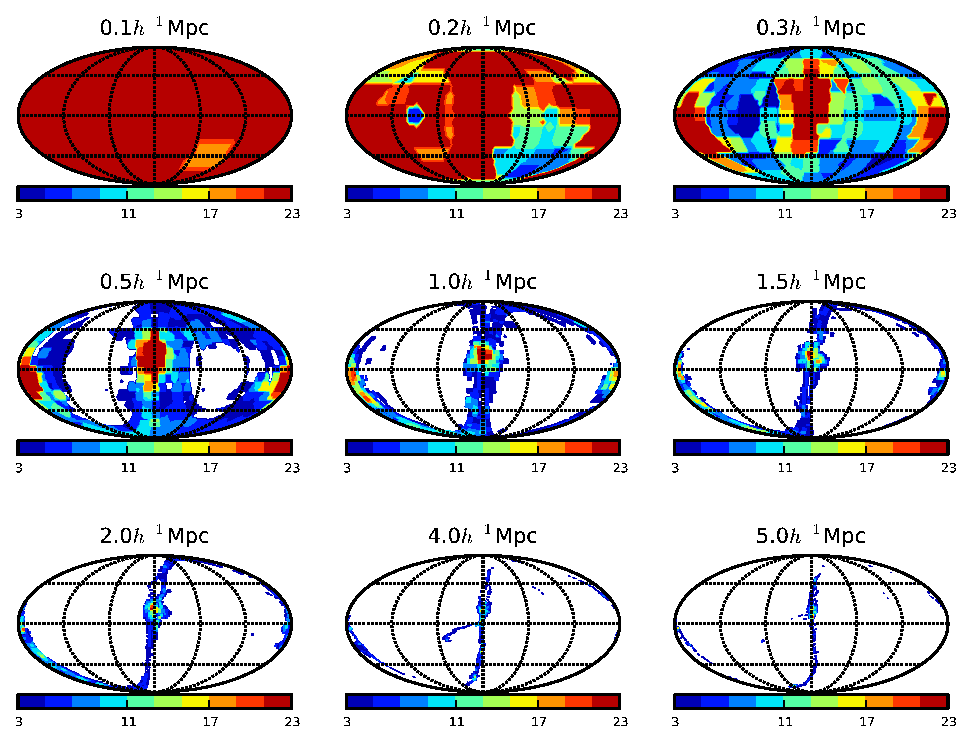
\includegraphics[width=10.cm]{Chapter3/Source_v2/fig9b} 
\end{minipage}\hfill
\caption{Halo of mass $7.0 \times 10^{12} M_{\odot} $  and  FOF radius 0.4 $h^{-1}$ Mpc. Top: All lines clearly scale between $r^{-1}$ and $r^{-2}$. Bottom: The filament is passing through the center. It persists from radius of halo to 4 $h^{-1}$ Mpc. It is also surrounded by a single wall appearing as a line in the middle.}
\label{fig:706}
\end{figure}



\begin{figure}
\begin{minipage}[t]{.99\linewidth}
  \centering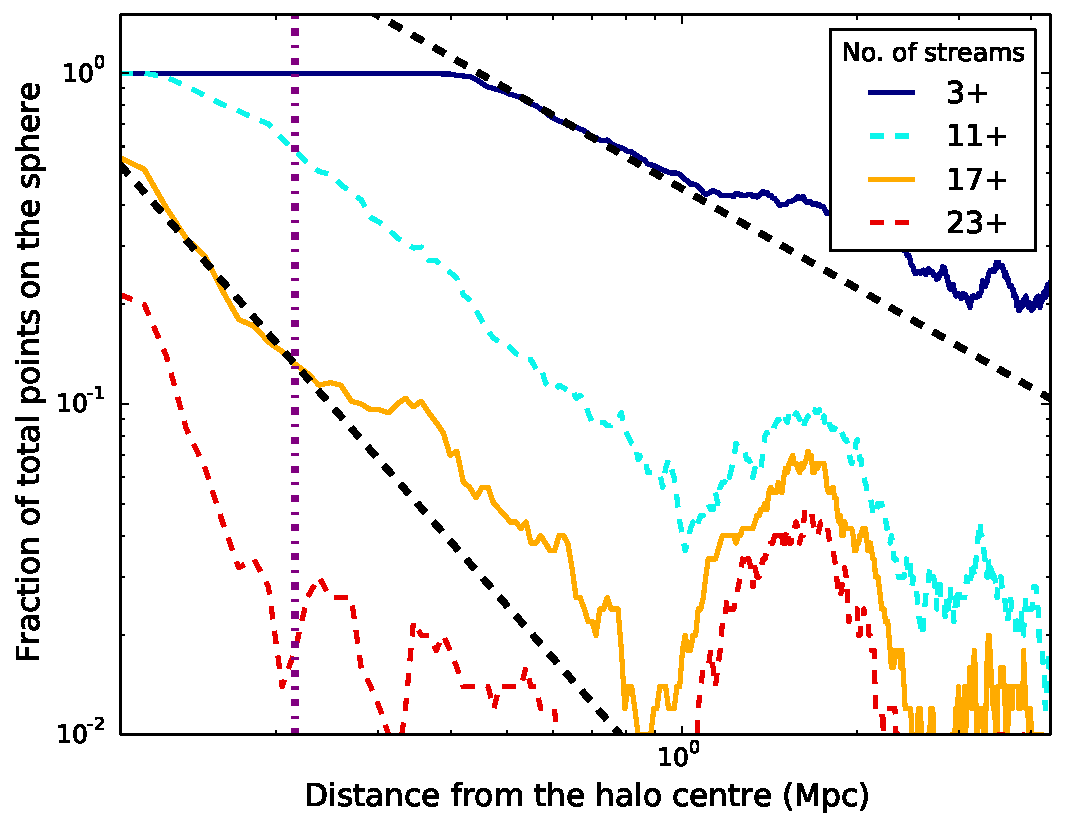
\includegraphics[width=10.cm]{Chapter3/Source_v2/fig10a}
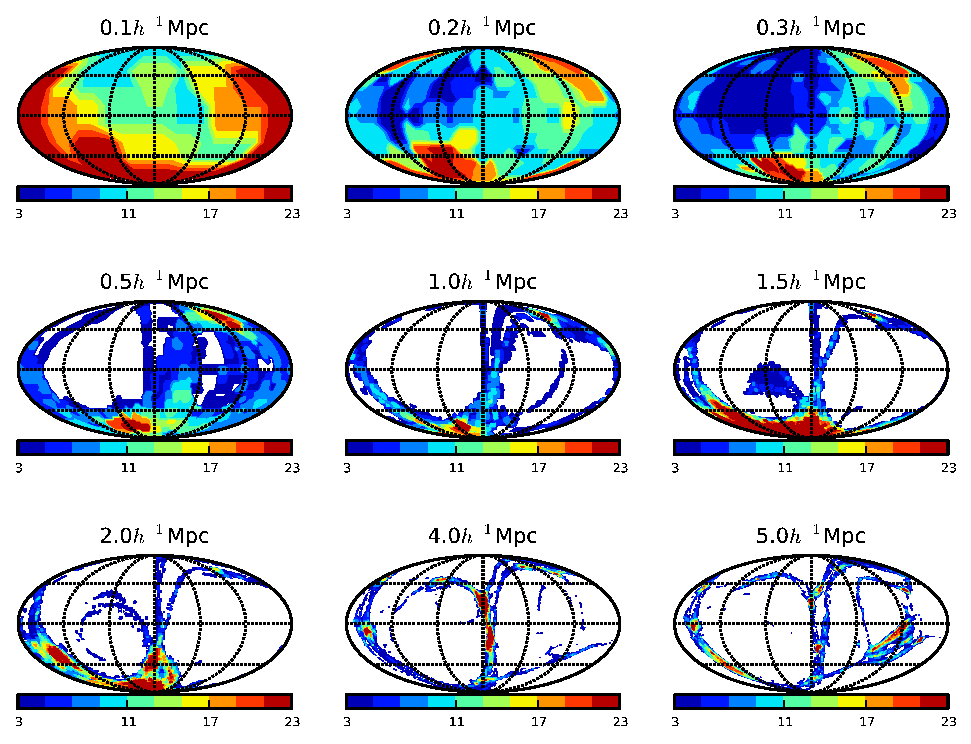
\includegraphics[width=10.cm]{Chapter3/Source_v2/fig10b}
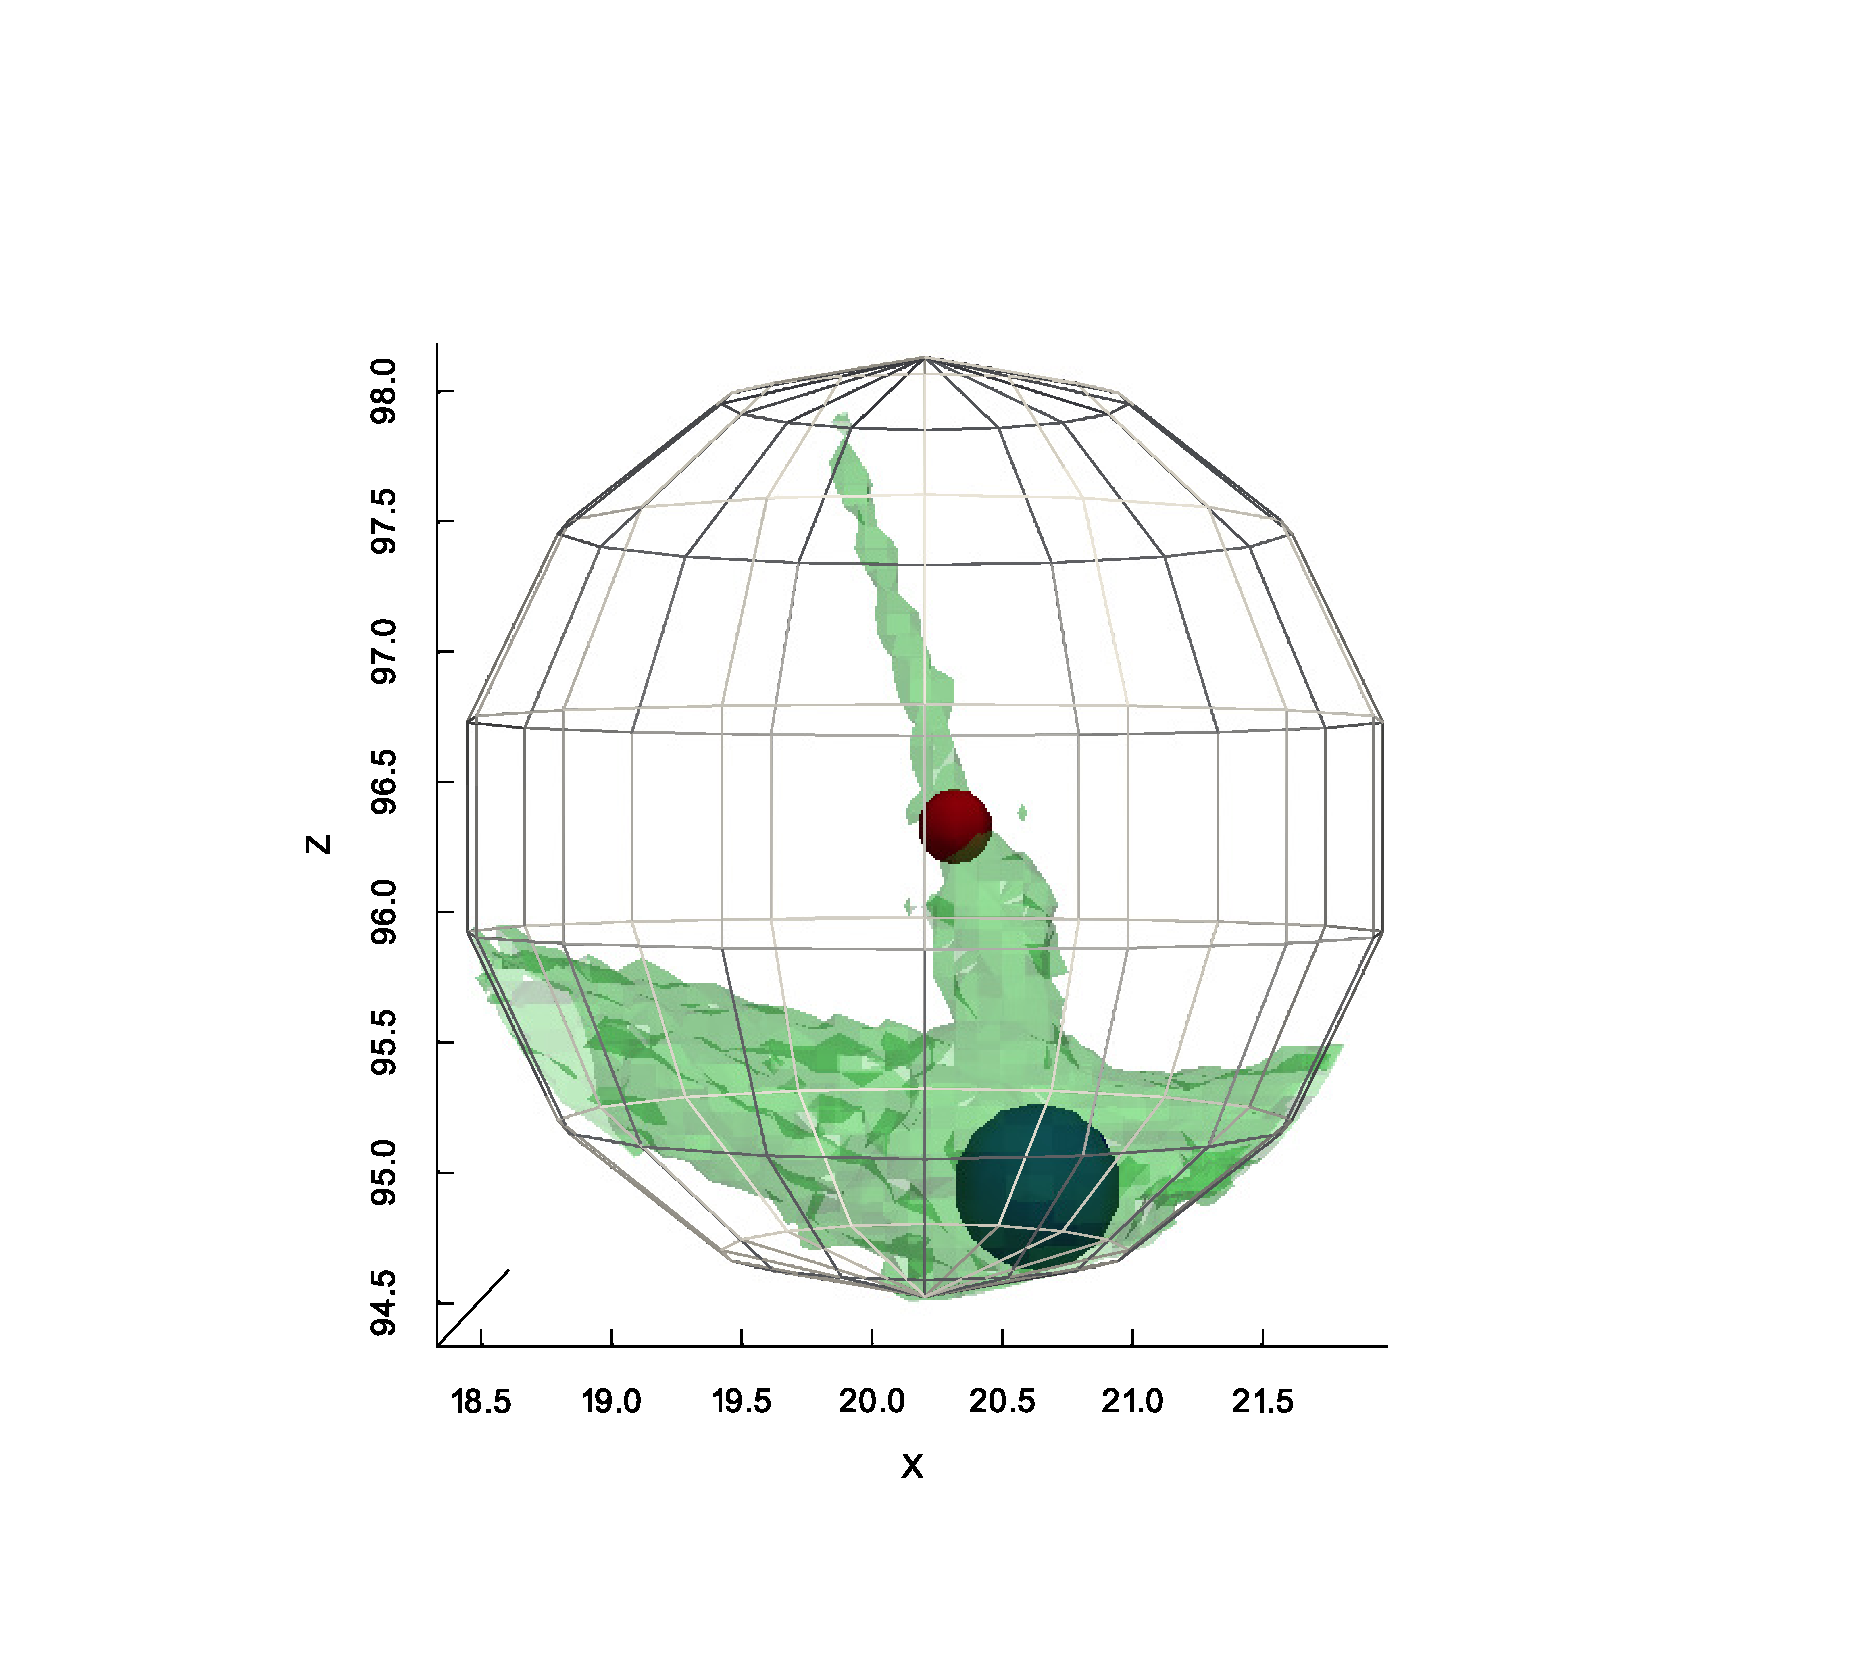
\includegraphics[width=6.cm]{Chapter3/Source_v2/fig10c}
\end{minipage}\hfill
\caption{Halo of mass $1.1 \times 10^{12} M_{\odot} $  and FOF radius 0.2 $h^{-1}$ Mpc (dotted-violet line). This halo just has 26 particles, hence the resolution is lesser than previous haloes for surfaces with low radii. Top: There is a bump in fraction of each of 3+ streams a little over 1 $h^{-1}$ Mpc. This is due to the presence of an additional halo nearby, as seen in the projections. The Mollweide projections from 0.4 $h^{-1}$ Mpc to 2 $h^{-1}$ Mpc have high stream flow regions near the lower surfaces of diagnostic spheres. Bottom: Corresponding FOF halo (red, at the center) has a more massive neighboring FOF halo (blue) within distance of 2 $h^{-1}$ Mpc. The 17+ stream regions (green) are increased around the neighboring halo.} 
\label{fig:4322}
\end{figure}

For illustrations, we have picked 4 haloes from different mass ranges: $3.7 \times 10^{14}M_{\odot} $,  $5.0 \times 10^{13} M_{\odot} $ , $7.0 \times 10^{12} M_{\odot} $ and $1.1 \times 10^{12} M_{\odot} $ from the simulation box of 100 $h^{-1}$ Mpc length and $128^3$ particles. Multi-stream field with a high refinement factor of 8 is calculated for a greater resolution on scales of the halo volume. Diagnostic spheres of radii 0.1 $h^{-1}$ Mpc to 5 $h^{-1}$ Mpc are drawn for each of these haloes (Figures ~\ref{fig:3} - ~\ref{fig:4322}; bottom figures), with the multi-stream field projected onto the surface. In the Mollweide projections of these spheres, the white space refers to single-stream voids. For the largest halo (Figures ~\ref{fig:3}) with FOF radii 1.2 $h^{-1}$ Mpc, the voids already appear in sphere of radius 1.5 $h^{-1}$ Mpc and in the smaller haloes (Figure \ref{fig:4322}) it appears as early as 0.5 $h^{-1}$ Mpc.  

Up to 1 $h^{-1}$ Mpc from halo center of the largest halo, the surfaces are uniformly covered with high number of streams (red, 17+). This shows that the most non-linear regions are close to centers of haloes. A similar trend is seen for the halo of radius 0.7 $h^{-1}$ Mpc (Figures ~\ref{fig:79}). However, for smaller haloes (Figures \ref{fig:706} and \ref{fig:4322}) lower number of streams (even the wall forming 3+ streams; blue) start occupying the spherical surface at radii lesser than FOF-radius. In the case of the smallest halo of $1.1 \times 10^{12} M_{\odot} $ mass, the 17+ streams are seen at scales as low as 0.1 $h^{-1}$ Mpc. The distribution of multi-streams on the surface seems do not have a symmetry of any kind , signifying a complex morphology of the web in the vicinity of the haloes. Regions with 5+ to 15+ streams form structures intermediary to filament-like and wall-like behavior, as seen by scaling of fraction of total points on the space with distance from halo center.

Halo environment at distance over twice the FOF radius reveals interesting morphological features. The walls intersect the sphere, and in the 
Mollweide projections, appear like a thin strip. 
We also note that a filament oriented tangentially to the diagnostic surface may occasionally appear as a strip too (like in Figure ~\ref{fig:79}, 
see the corresponding discrepancy in fraction of streams), but upon inspecting the spheres at various radii, we can clearly identify the persisting line-like structures, and they correspond to the walls. Similarly, a filament is projected as a compact patch structure, which occurs due to an intersection of a cylinder-like geometry with the spherical surfaces. It is clearly observed at the distance of 4 - 5 $h^{-1}$ Mpc in Figure \ref{fig:3} and in between 0.5 - 5.0 $h^{-1}$ Mpc in Figure \ref{fig:706}.
	
Hence we conclude that the 3+ stream regions constitute predominantly walls and the regions with 17+ streams correspond mostly to filaments. The higher $n_{str}$ shells must be surrounded by the layers with lower $n_{str}$. Thus, the filaments are within the walls, and do not exist independently.  
We remind that the radius of diagnostic sphere varies from 0.1 - 5 $h^{-1}$ Mpc, whereas the Mollweide projections shown here are of the same size. Hence the walls and filaments appear more narrow and smaller in larger spheres due to zooming-out effects. 
 In some cases (Figures \ref{fig:79}, ~\ref{fig:4322}), the Mollweide projections display the walls  and filaments as a complicated network 
 with patches of high number of streams. 

The high peak shown by the curves corresponding to the numbers of streams from 11+ to 17+  in the top panel of Figure ~\ref{fig:4322}
is mostly due to the presence of another halo nearby ( seen at bottom of Mollweide projection of 1 - 2 $h^{-1}$ Mpc). Figure \ref{fig:79} also has a deviation from usual scaling, and this due to the intricate shape of 17+ stream filament, which appears to be branching out after 1 $h^{-1}$ Mpc. 

Generally the transitions from haloes to filaments then to walls and finally to voids appear to be rather smooth.
However occasionally sharp features as the one seen in Figure ~\ref{fig:4322} may emerge when the diagnostic sphere hits a neighboring halo.

% \begin{figure}
% \begin{minipage}[t]{.99\linewidth}
%   \centering\includegraphics[width=10.cm]{fig11} 
% \end{minipage}\hfill
% \caption{Variation of fraction of stream around haloes on sphere of radius calculated from FOF. 10 haloes are considered for each mass range.}
% \label{fig:SphFr}
% \end{figure}
 
 
 \begin{figure}
\begin{minipage}[t]{.99\linewidth}
  \centering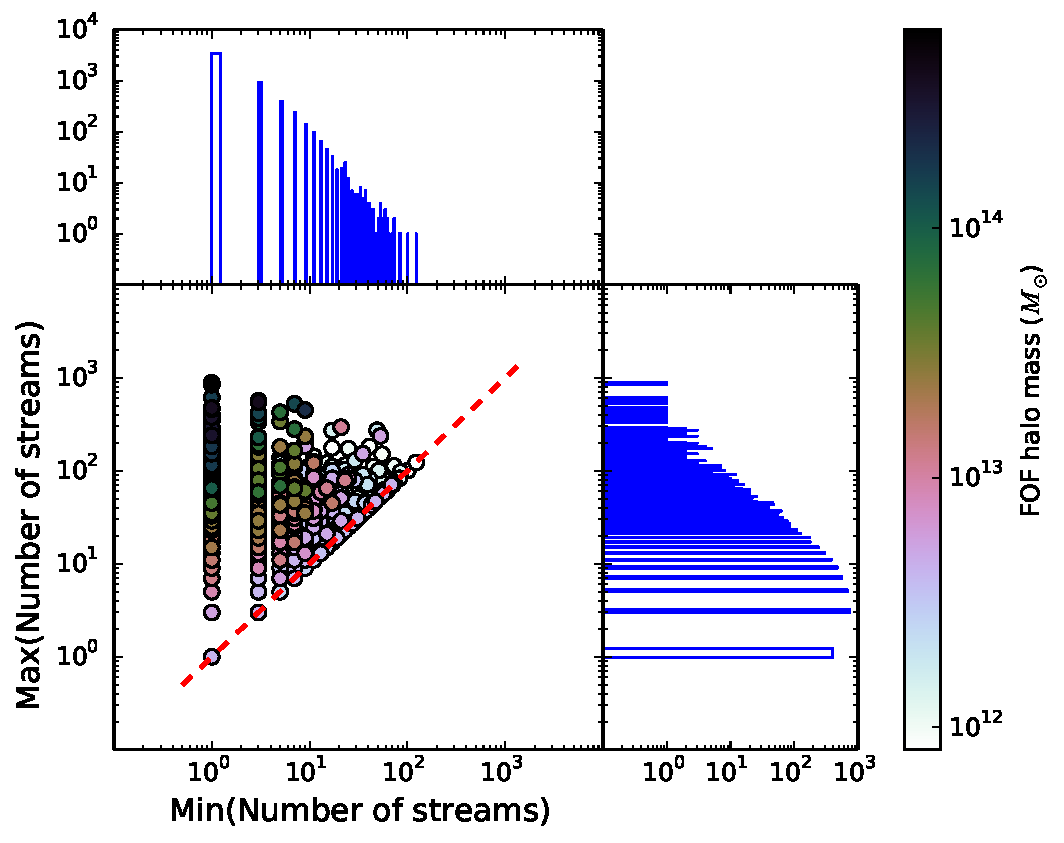
\includegraphics[width=10.cm]{Chapter3/Source_v2/fig11a}
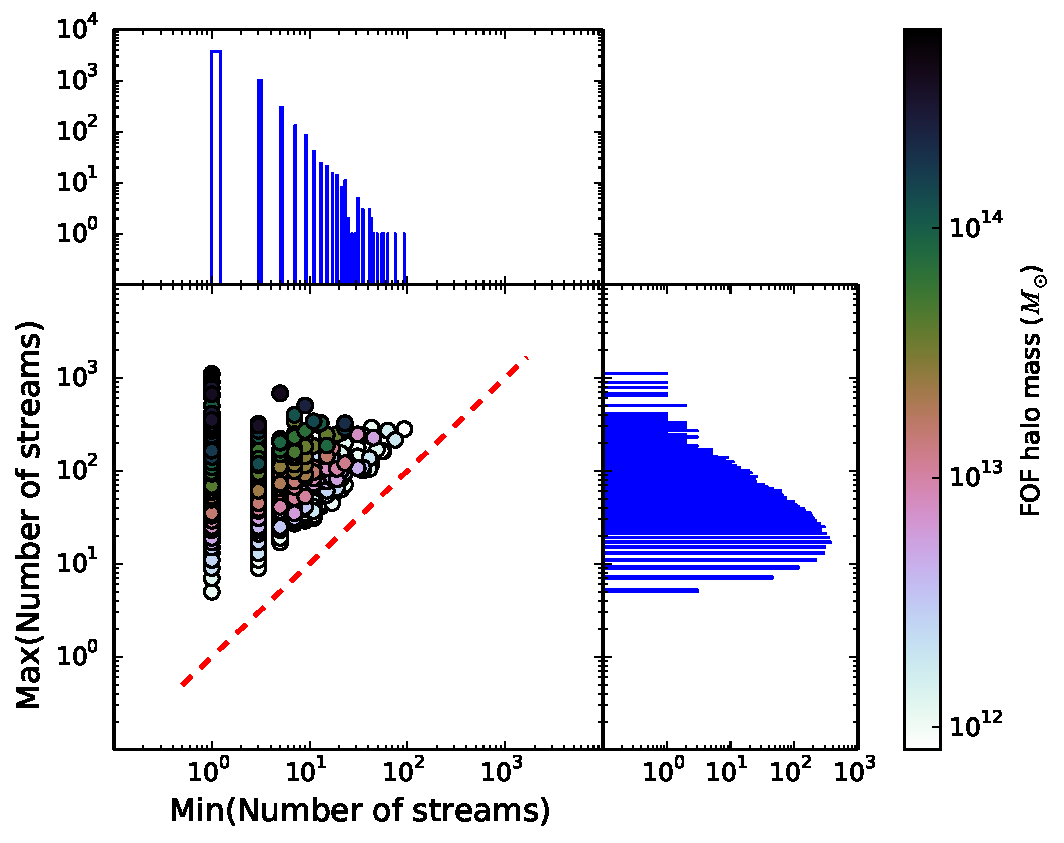
\includegraphics[width=10.cm]{Chapter3/Source_v2/fig11b} 

\end{minipage}\hfill
\caption{Scatter plot of minimum and maximum number of streams on the surface of FOF radius around all haloes in FOF catalog. For the analysis, we use a total of 5521 haloes that are identified using the FOF technique with linking length, $b=0.2$. Since several of the haloes coincide, distributions of number of haloes corresponding to minimum and maximum $n_{str}$ on their FOF radii are shown above and beside the scatter plot respectively. Top: Full box of $L =100 ~h^{-1}$ Mpc and $N = 128^3$ (i.e. $L/N = 0.78 \,h^{-1}$), with a low refinement factor of 1 is utilized for multi-stream field calculation. Bottom: Same simulation box; multi-stream field calculated with higher refinement factor of 8.}
\label{fig:minmax128}
\end{figure}

 \begin{figure}
\begin{minipage}[t]{.99\linewidth}
  \centering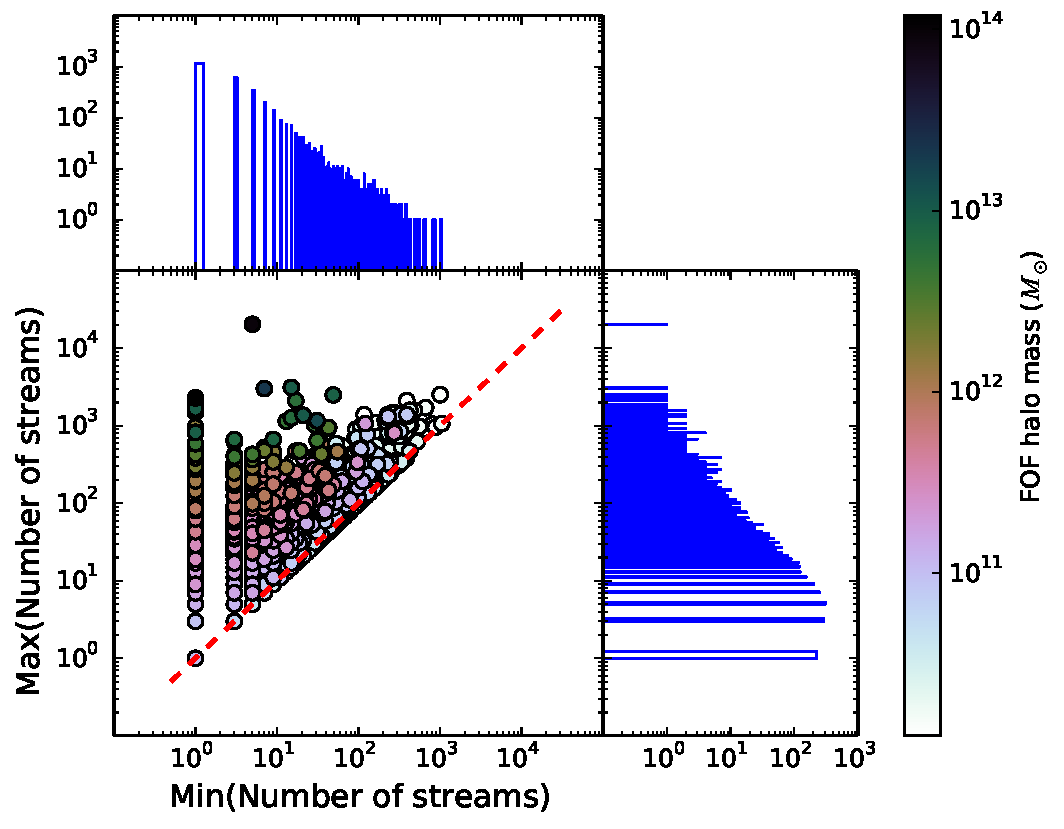
\includegraphics[width=10.cm]{Chapter3/Source_v2/fig12a}
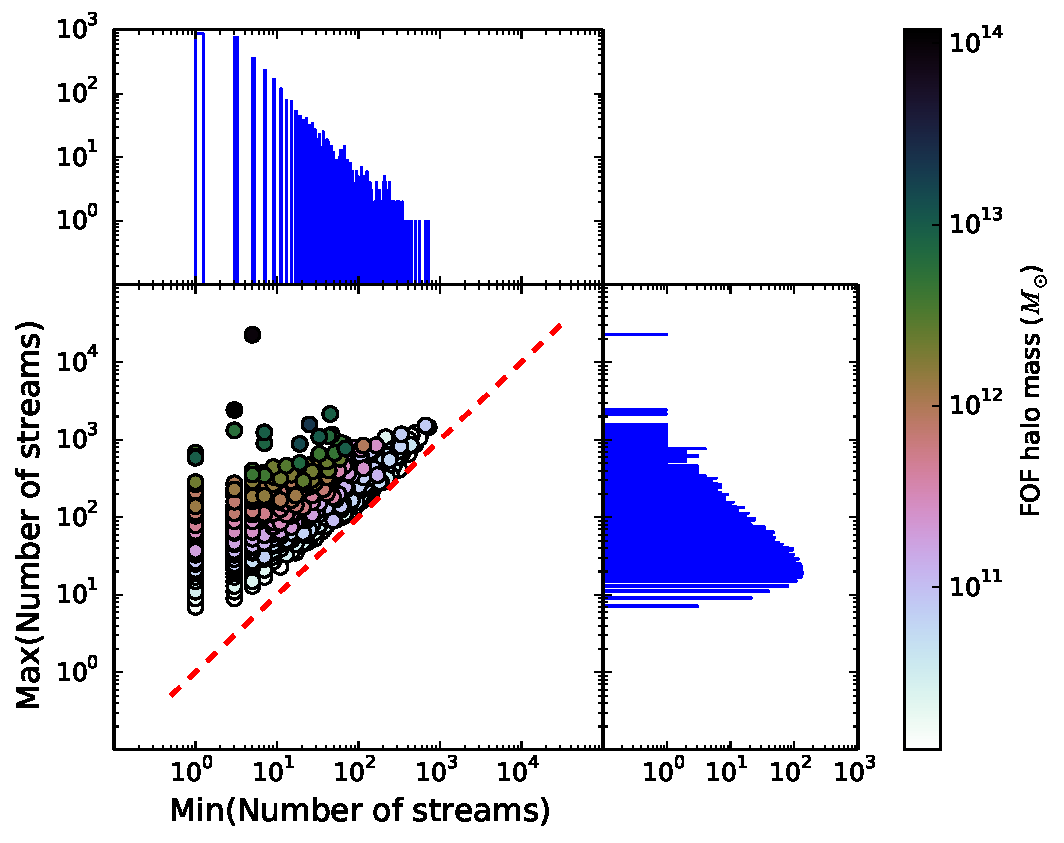
\includegraphics[width=10.cm]{Chapter3/Source_v2/fig12b} 
\end{minipage}\hfill
\caption{Scatter plot of minimum and maximum number of streams on the surface of FOF radius around all haloes in FOF catalog. Distributions of number of haloes corresponding to minimum and maximum $n_{str}$ on their FOF radii are shown above and beside the scatter plot respectively. Top: In the simulation box of $L =100 ~h^{-1}$ Mpc and $N = 512^3$ (i.e. $L/N = 0.19 \,h^{-1}$), multi-stream field is calculated on a smaller slice of $ 25 ~h^{-1}$ Mpc is  with a refinement factor of 1. Multi-stream field is projected onto surfaces of 3448 FOF haloes within this small box. Bottom: Same simulation box; the multi-stream field calculated on the the same small box, but with a refinement factor of 8.}
\label{fig:minmax512}
\end{figure}

The friends-of-friends analysis identifies haloes as spherical structures. The distribution of multi-streams projected onto these surfaces of the FOF haloes can be utilized for a statistical analysis of the haloes (Figures \ref{fig:minmax128} and \ref{fig:minmax512}). We have utilized FOF catalogs of haloes more than 20 particles found at linking length $ b= 0.2$.  The $n_{str}$ ranging from as low as 1 to higher than 10$^3$ are seen on the halo surfaces. Haloes which have the minimum $n_{str} = 1$ are in contact with the void. However, if the maximum $n_{str}$ is also 1, then the halo is completely within the void. In calculations with low refinement factor of 1, only 7.3$\%$ (for  $L/N = 0.78 \,h^{-1}$) and 6.5$\%$ (for  $L/N = 0.19 \,h^{-1}$) of the haloes are completely within single streaming voids. This is solely due to low resolution of multi-stream field, since none of the FOF haloes are found in high resolution multi-stream calculations on both $L/N = 0.78 \,h^{-1}$ and $L/N = 0.19 \,h^{-1}$ boxes. At high refinement factors, none of the haloes are entirely embedded in a region with just one multi-stream value (i.e., max($n_{str}$) = min($n_{str}$), along the dotted-red lines in Figures \ref{fig:minmax128} and \ref{fig:minmax512}). However, there are significant number of haloes whose FOF surfaces are in contact with the void region: in calculations with refinement factor of 8, 62$\%$ of the haloes in $L/N = 0.78 \,h^{-1}$ and 34$\%$ of the haloes in $L/N = 0.19 \,h^{-1}$ are in contact with void on their FOF radii. Rest of the haloes are completely within non-void regions.

Statistical analysis of FOF haloes in Figures \ref{fig:minmax128} and \ref{fig:minmax512} show that massive haloes tend to have low min($n_{str}$) and high max($n_{str}$), hence a very diverse multi-stream environment on their spherical surface. The heuristic  multi-stream threshold for haloes mentioned in Section \ref{sec:global} results in virialized haloes with a constant $n_{str}$ value. These halo surfaces far from sphere (see Figures \ref{fig:4view}), whereas, the FOF surfaces are spherical and have a large range of number of streams on their surfaces. The probability distribution function of number of FOF haloes has an approximately exponential tail monotonically decreasing with with min($n_{str}$). 


%The probability distribution function of the number of streams on the diagnostic sphere of the FOF radius is shown in  \hl{Fig. \ref{fig:minmax128} Text to be changed}. It is computed  from a sample of 10 haloes in four mass ranges. As expected, the highest number of streams is observed in the vicinity of the most massive haloes. 
% Over 200 streams has been observed in the case of the haloes with masses  in the range $ 2.1 \times 10^{14}  - 3.9 \times 10^{14}  M_{\odot} $. The smallest haloes with mass $1.1 \times 10^{12}  M_{\odot} $ the highest number of stream on the FOF radius (0.2 $h^{-1}$ Mpc) is less than 50. Note that a large number of small haloes are detected by FOF with just 26 particles, hence all ten haloes have the same mass. The shapes of the curves suggest that the probability distribution function of the number of streams on the diagnostic sphere of the FOF radius has exponential tails monotonically increasing with mass. A relatively large range of the number of streams indicates that the number of streams field in the vicinity of the haloes is far from spherical.



\section{Summary}
In this chapter, we discuss the results of the first study of the multi-stream environment of dark matter haloes in cosmological N-body simulations.
%We study the multi-stream field computed in N-body simulations in $\Lambda$CDM cosmology at $z=0$.
The visualization and quantitative characterization of generic non-linear fields in three-dimensional space represent a serious
challenge from both conceptual and computational points of view. The complexity of the problem requires diverse tools
for analyzing the results of cosmological simulations as well as galaxy catalogs.


This study is different from the most previous works in a few aspects.
Firstly, we consider the representation of the cosmic web in the form of  a multi-stream field rather  than a density field.
The multi-stream field contains a different information about the web than the density and velocity fields and thus represents 
a complimentary characterization of the web revealing new dynamical features of the web 
(\citealt{Shandarin2011}, ~\citealt{Shandarin2012},~\citealt{Abel2012}).  Secondly, for computing the multi-stream field we use 
the tessellation of three-dimensional Lagrangian sub-manifold ${\bf x} = {\bf x}({\bf q}, z=0)$ in six-dimensional $({\bf x},{\bf q})$ space
which allows to significantly increase the spatial resolution (\citealt{Shandarin2012},~\citealt{Abel2012}). The Lagrangian sub-manifold is more convenient since
{\bf x}  is a single-valued function of {\bf q} at any stage including a highly non-linear regime while 
the phase space sheet projected on  {\bf x}- or {\bf v}-space is not. If the initial state of the simulation is represented by a uniform three-dimensional mesh, then storing the Lagrangian sub-manifold does not require additional space for Lagrangian coordinates. And thirdly, in the study of the multi-stream environment of dark matter haloes we use the Mollweide projection of the multi-stream field 
computed on a set of diagnostic spherical surfaces centered at the FOF haloes and  having radii from 0.1 $h^{-1}$Mpc to 5 $h^{-1}$Mpc.

Most of the results are obtained for a simulation in $L=100  h^{-1}$Mpc box with $N = 128$  particles along each axes although we report
some of the results for the simulations in 100  $h^{-1}$Mpc box with 256$^3$ and 512$^3$ particles as well as  in 200  $h^{-1}$Mpc
box with 128$^3$, 256$^3$  and 512$^3$ particles.

Using the tessellation of the three-dimensional Lagrangian sub-manifold 
${\bf x} = {\bf x} ({\bf q},t)$  \citep{Shandarin2012}, we compute the multi-stream field i.e. 
the number of streams  on a regular grid in the configuration ${\bf x}$-space, $n_{str}({\bf x})$ for
estimating global parameters or on selected set of points in the study of the haloes environments.

The multi-stream field takes odd whole numbers everywhere except at a set of points of measure zero where it takes positive even whole numbers.
This property is very useful for debugging the numerical code.

 The multi-stream field allows one to define physical voids as the regions with $n_{str} =1$. 
 The rest of space with $n_{str} \ge 3$ can be called the non-void or web.
This division of the space into two parts is unique and physically motivated: no object can form before shell crossing happens. 
It is worth emphasizing that the division of space into voids and web is based on the local parameter, the number of streams at a single point (\citealt{Shandarin2012}, \citealt{Abel2012}). \citet{Falck2012} and \citet{Falck2015} defined the web as a set of particles that experienced the 'flip-flop' at least once along any axis. We discussed potential problems with this definition in the beginning of Section \ref{sec:global}.




%\citet{Falck_etal:12} and \citet{Falck_Neyrinck:14} used similar physical idea in the ORIGAMI method, \hl{but their numerical method is different and a little less accurate. HOW?? (Ignore this sentence?)} 
   
 The further division of the web into walls, filaments and haloes is not straightforward although haloes can be defined using dynamical parameters
 related to the requirement of virialization of haloes. One of the simplest is the famous density threshold $\rho/\bar{\rho} \approx 200$. 
 Identifying filaments and walls is significantly more tricky (see e.g. \citealt{Hahn2007}, \citealt{Forero-Romero2009a}, 
  \citealt{Aragon-Calvo2010a}, \citealt{Cautun2014a}, \citealt{Falck2015}) and require non-local parameters.
  
The large part of walls can also be identified locally since the regions where $n_{str} = 3$ can be neither filaments nor haloes. 
For instance, in the simulation  100  $h^{-1}$Mpc box with 128$^3$  particles the web occupies about 6\% of the volume, the three-stream flow
regions occupy about 4\% and the rest of the web remaining 2\% of the total volume.

In this study we introduced an empirical statistical criteria which very crudely distinguish wall, filament and haloes. %for identifyinh filaments and walls.
We have found empirically that  in  the studied simulation the transition from wall points to filament points takes place approximately at $ 5 \le n_{str} \lesssim 15$. Using the virial over-density threshold of 200 in Eq.~\ref{eq:den}, we have also estimated that the haloes correspond to the regions with $n_{str} \gtrsim 90$.
Thus, the transition from filament to haloes takes place in the range $ 17 \le n_{str} \lesssim 90$.
The above critical values for transition from walls to filaments and from filaments to haloes were shown to be approximately correct
for  the simulation with $L/N = 0.78 h^{-1}$ Mpc. This technique can be also applied to simulations with different $L/N$ ratio and multi-stream grid of different refinement factors but the classification based on the threshold applied locally will remain only a very crude estimator. A more sophisticated morphological analysis will require non-local geometric and topological methods, which is discussed in Chapters \ref{chapter4} and \ref{chapter5}.  
 
 \begin{table*}
 \centering
  \caption{Comparison of the volume and mass fraction of the elements of the cosmic web between our analysis and \citet{Falck2015}. $ L/N = 0.78 h^{-1}$ Mpc for simulations used in both techniques. We use a refinement factor of 8 for the multi-stream grid. The mean density is given in units of the mean density of the universe. }
\begin{tabular}{|l|r|r|r|r|r|r|r|r|}
\hline
\multicolumn{1}{|c|}{} & \multicolumn{4}{l|}{Multi-stream analysis (This work)} & \multicolumn{4}{c|}{ORIGAMI \citep{Falck2015}}    \\ \hline
                       & Voids & Walls & Filaments & Haloes  & Voids & Walls & Filaments & Haloes \\ \hline
Volume Fraction (\%)                 & $93$   & $7$    & $< 1$      & $< 0.1$ & $84$   & $12$   & $3$        & $< 1$  \\ \hline
Mass Fraction   (\%)               & $32$   & $35$   & $17$       & $14$    & $26$   & $19$   & $19$       & $35$   \\ \hline
Mean density                    & $0.34$ & $5$    & $>17$      & $>140$  & $0.31$ & $2.2$  & $6$        & $>35$  \\ \hline
\end{tabular}
 \label{tab:Compare}
\end{table*}

We have found that the volume and mass fractions in the voids  are approximately V.F./M.F. = 96/76, 93/32  and 88/24, where each number
is the percentage, for the simulations with  $L/N = 1.56 \,h^{-1}$, $0.78 \,h^{-1}$  and $0.19 \,h^{-1}$ Mpc respectively. As the ratio $L/N$ 
gets smaller both volume and mass fractions in  voids monotonically decrease.  
This is fairly consistent with the results of \citet{Falck2015}, considering the differences between our numerical methods. We compare the fractions of the volumes and masses in other components of the web in Table \ref{tab:Compare}, and the results are in a good qualitative agreement.
Our estimates systematically higher for both volume and mass fractions for voids and thus systematically lower for the web. 
One general conclusion seems to be obvious: the web defined by the multi-stream flows is about  (100\% - 84\%)/(100\%-93\%)=2.3  times  thinner than that defined by the ORIGAMI  method. 


%\begin{table}
%\begin{tabular}{|l|c|c|c|c|}
%\hline
%     & Void        & Wall    & Filament & Halo       \\ \hline
%V. F. & $93$ / $84  $   & $7$ / $12$  & $< 1$ / $3$  & $< 0.1$ /$ <1$ \\ \hline
%M. F. & $32$ / $26 $    & $33$ / $19$ & $19$ / $19$  & $14$ / $35$    \\ \hline
%$\bar{\rho}$     & $0.34$ / $0.31$ & $5$ / $2.2$ & $>19$ / $6$  & $>140$ / $>35$ \\ \hline
%\end{tabular}
% \caption{Comparison of the volume and mass fraction of the elements of the cosmic web between our analysis and \citet{Falck_Neyrinck:14}. $ L/N = %0.78 h^{-1}$ Mpc for simulations used in both techniques.  }
% \label{tab:Compare}
%\end{table}




In conclusion we would like  to outline the major aspects of the web revealed by the study of the multi-stream field.
The multi-stream field is a fundamental attribute of the structures formed in cold collision-less dark matter. Its properties
are of great importance for the detecting dark matter directly in a laboratory setting or indirectly via astronomical observations.
The dark matter web described by a multi-stream field represents a nested structure, consisting of layers with increasing number of streams.
The number of streams are odd integers almost everywhere except on caustics where they are even integers.
The caustics occupy infinitesimal volume. The most of the volume is occupied by one stream flow regions which
are dark matter voids. The regions with three streams are the regions occupying the second largest volume.
They form very thin membrane type structures (often referred to as walls or pancakes) most of which are connected 
in one huge connected formation. The three-stream regions form the external shell of the web. All other structures
filaments and haloes are within the three-stream shell. The membranes are attached to each others by the filaments which locally consist of regions with higher number of streams  than the neighboring membranes. The filaments form the framework or a skeleton of the dark matter web.  Similar to a real skeleton, the filamentary structure has joints where most of the the dark matter haloes are located. The haloes are the local peaks of the multi-stream field.




% \section*{Acknowledgements}
% The authors are grateful to Gustavo Yepes and Noam Libeskind for providing the simulations used in this study and the Sir John Templeton Foundation for the support.The authors would also like to thank the anonymous referee for careful review and useful suggestions.


%\bibliographystyle{mn2e}
%\bibliography{bibliography}

%\end{document}

% \mathbf -> \mathbf
% \mathbfss{H} -> {\bf H}
% \sun -> \odot

\begin{comment}
\documentclass[fleqn,usenatbib,useAMS]{mnras}
%\documentclass[referee,fleqn,usenatbib,useAMS]{mnras}

\pdfoutput=1 
\pdfminorversion=5 


\usepackage{amssymb}
\usepackage{amstext}
\usepackage{amsmath}
\usepackage{epsf}
\usepackage{graphicx}
\usepackage{graphics}
\usepackage{epsfig}
\usepackage{wrapfig}
\usepackage{listings}
\usepackage{float}
\usepackage{esint}
\usepackage{natbib}
\usepackage{ifthen}
\usepackage{hyperref}
\usepackage{verbatim}

% ----------HIGHLIGHTING -------
\usepackage{xcolor}
\usepackage[normalem]{ulem} % use normalem to protect \emph
\newcommand\hl{\bgroup\markoverwith
  {\textcolor{yellow}{\rule[-.5ex]{2pt}{2.5ex}}}\ULon}

\newcommand\rhl{\bgroup\markoverwith
  {\textcolor{orange}{\rule[-.5ex]{2pt}{2.5ex}}}\ULon}
  
 \newcommand\ghl{\bgroup\markoverwith
  {\textcolor{green}{\rule[-.5ex]{2pt}{2.5ex}}}\ULon} 
%-------------------------------------------------------------------------
%-------------------------------------------------------------------------
\begin{document}
\label{firstpage}
\pagerange{\pageref{firstpage}--\pageref{lastpage}}

\title[Topology and geometry of the dark matter web]{Topology and geometry of the dark matter web: a multistream view}

\author[Ramachandra \& Shandarin]
	{Nesar S. Ramachandra, \thanks{E-mail: nesar@ku.edu} 
	Sergei F. Shandarin, \\
	Department of Physics and Astronomy, University of Kansas, Lawrence, KS 66045}



\maketitle
%-------------------------------------------------------------------------------------------
\begin{abstract}

Topological connections in the single-streaming voids and multistreaming filaments and walls reveal a cosmic web structure different from traditional mass density fields. A single void structure not only percolates the multistream field in all the directions, but also occupies over 99 per cent of all the single-streaming regions. Sub-grid analyses on scales smaller than simulation resolution reveal tiny pockets of voids that are isolated by membranes of the structure. For the multistreaming excursion sets, the percolating structure is significantly  thinner than the filaments in over-density excursion approach.  

Hessian eigenvalues of the multistream field are used as local geometrical indicators of dark matter structures. Single-streaming regions have most of the zero eigenvalues. Parameter-free conditions on the eigenvalues in the multistream region may be used to delineate primitive geometries with concavities corresponding to filaments, walls and haloes.


% We also introduce, for the first time, a framework to detect dark matter haloes in multistream fields. Closed compact regions hosting local maxima of the multistream field are detected using local geometrical conditions and properties of the Lagrangian sub-manifold. All the halo particles are guaranteed to be completely outside void regions of the Universe. Majority of the halo candidates are embedded in the largest structure that percolates the entire volume.


\end{abstract}

\begin{keywords}
methods: numerical -- cosmology: theory -- dark matter -- large-scale structure of Universe 
\end{keywords}

\begingroup
\let\clearpage\relax
%\tableofcontents
\endgroup
\newpage
\end{comment}
%-------------------------------------------------------------------------------------------------------------------------------
\chapter{Topology and geometry of the dark matter web}\label{chapter4}

Heuristic analysis of the multistream field has been done in Chapter \ref{chapter3} and parts of Chapter \ref{chapter3b}. In this chapter, we analyse the dark matter structures based on their phyiscal shapes and connectivity. Extensive studies of geometrical and topological properties in cosmic matter density field have been done in the past. Here we extend some of these studies into the Lagrangian sub-manifold regime -- taking advantage of certain unique properties of the multistream field supplement our understanding of dark matter structures. The analysis and text in this chapter overlaps with \cite{Ramachandra2017}.   


\section{Introduction} 
\label{sec:intro}


% Large scale structures with  highly anisotropic shapes were first theoretically predicted by Zeldovich approximation (hereafter ZA) \citep{Zeldovich1970}. The model based on ZA suggested that the eigenvalues of the deformation tensor dictate the shapes of the {\it collapsed} structures at the beginning non-linear stage of gravitational instability (\citealt{Arnold1982}, see also \citealt{Shandarin1989} and \citealt{Hidding2014}). These structures were found to be crudely  characterised as two-, one- and zero- dimensional  which actually meant that three characteristic scales of each structure ($L_1\ge L_2\ge L_3$) are approximately related as  $L_1^{(p)} \approx L_2^{(p)} \gg L_3^{(p)}$ or $L_1^{(f)} \gg L_2^{(f)} \approx L_3^{(f)}$ or $L_1^{(h)} \approx L_2^{(h)}  \approx L_3^{(h)} $ respectively.  In addition it implied that $L_1^{(p)} \approx L_1^{(f)}$ and $L_3^{(p)} \approx L_2^{(f)} \approx L_1^{(h)}$.\footnote{The multi-scale character of the cosmic web was not discussed until 1990s.} At present these generic types of structures are referred to as  walls/pancakes/sheets/membranes, filaments and haloes. Although the accuracy of the Zeldovich approximation deteriorates from pancakes to  filaments and especially to halos on qualitative level  there are no more types of  structures. Altogether these structures contain the most of mass in the universe nevertheless they occupy  very little space. The most of space is almost empty  and is referred to as voids.
% 
% \cite{Klypin1983a} (firstly reported  in \citealt{Shandarin1983}) were the first to identify a `three dimensional web structure' in the N-body simulation of the hot dark matter scenario. The simulation with $32^3$ particles used Cloud-in-Cell (CIC) technique on equal mesh revealed  that the gravitationally bound clumps of mass -- haloes in the present-day terminology --  were linked by the web of filamentary enhancements of density which spanned throughout the entire simulation box with the side of about 150$h^{-1}$Mpc in co-moving space. In addition \cite{Klypin1983a}  suggested that pancakes must be considerably less dense than the filaments since they were not detected in the simulation. These  results were quickly confirmed by \cite{Centrella1983} and \cite{Frenk1983}. In addition \cite{Centrella1983} who ran the simulation on similar mesh but with 27 times more particles also detected pancakes at $\rho/\bar{\rho} = 2$ level. At present this picture is widely accepted, and is referred to as the `cosmic web' (\citealt{Bond1996} and \citealt{Weygaert2008c}). 
% 
% Galactic distributions in redshift surveys have also revealed distinct geometries and topologies of the cosmic web. One of the first indications of the connection of the clusters of galaxies by filaments was demonstrated by \cite{Gregory1978} who discovered a conspicuous chain of galaxies between Coma and A1367 clusters using a sample of 238 galaxies. Later  this result was confirmed by \cite{Lapparent1986} who used a significantly greater redshift catalogue of 1100 galaxies of the same region. \cite{Zeldovich1982} compared the percolation properties of the redshift catalogue of 866 local galaxies provided by J. Huchra with three theoretical distribution of particle in space: a Poisson distribution, the  hierarchical model by \cite{Soneira1978} and the particle distribution obtained from N-body simulation by \cite{Klypin1983a}.  They found that the both the galaxy sample and the density field obtained in N-body simulation percolated at considerably smaller filling factors  than  the Poisson distribution. On the other hand the  hierarchical model percolated at higher filling factors  than  the Poisson distribution. Further studies confirmed that the galaxies and the particles in the hot dark matter  model are arranged in the web-like structures \cite{Zeldovich1982}, \cite{Shandarin1983}, \cite{Shandarin1983b}, \cite{Shandarin1984}. This result was confirmed in more detailed analysis by \cite{Einasto1984}. \cite{Melott1983b} also found similar percolation properties in the mass distribution in the N-body simulation of a CDM model.
%  
% Thus by the  early 1990s it was clearly demonstrated that the web like structure is a generic type for a wide range of initial conditions in both two-(\citealt{Melott1990}, \citealt{Beacom1991}) and three- dimensional \citep{Melott1993} cosmological N-body simulations. However it also was demonstrated that the quantitative parameters of the web structures depend on the initial  power spectrum. Remarkably the simulations also showed that  adding small scale perturbations does not ruin the large scale structures if the slope of the power spectrum is negative in both two- and three- dimensional simulations.
% 
% All aspects of these studies have been experiencing great advancements in  three decades passed since the discovery and first studies of the geometry and topology  of the large-scale structures. The galaxy redshift catalogues have grown by thousands of times (by surveys such as Sloan Digital Sky Survey (SDSS) \citealt{Tegmark2003} and \citealt{Albareti2016} and the 2MASS Redshift Survey \citealt{Huchra2012}), the sizes of cosmological N-body simulations (modern large scale simulations like Millennium \citealt{Springel2005b} and Q-Continuum \citealt{Heitmann2015}) by more than a million times. The number of various methods for identifying  structures has also grown practically from  one method\footnote{FOF was used for the topological studies via percolation technique and identifying super clusters of galaxies (\citealt{Zeldovich1982}, \citealt{Shandarin1983}, \citealt{Shandarin1983b} on the one hand and for identifying halos \citealt{Davis1985} on the other.}  to several dozens (\citealt{Colberg2008}, \citealt{Knebe2011a}, \citealt{Onions2012}, \citealt{Knebe2013} and references therein). Measuring or quantifying  the structures always has  been a difficult problem and many sophisticated  techniques both mathematically and computationally have been proposed and investigated (see reviews by \citealt{Weygaert2008c}, \citealt{Weygaert2008}).
% 
% \begin{comment}
% 
% Most of structure finders are halo finders only and most of them are stemmed from three types suggested long ago.
% One of them is the SO (Spherical Over-density) halo finder that defines halos  as spherical regions whose mass density 
% exceeds the mean density by a specified factor \citep{Press1974}. 
% Another is the FOF  (Friends-of-Friends) halo finder describing haloes  as the groups of particles separated less than 
% a specified linking length often chosen as 0.2 times the mean particle separation \citep{Davis1985}.
% Finally the DENMAX (DENsity MAXimum) halo finder assumes that the halos are the peaks of the density  fields
%  and thus selects the particles concentrated in the vicinity of the density maxima \citep{Bertschinger1991}.
% One of the common features of these  techniques is that all three are density based in one form or another.  
% And all of them depend on free parameters that are chosen chiefly on the `merits principle' \citep{Forero-Romero2009a} 
% rather than on physics.   Over the years all three kinds of the halo finders have been experiencing various modifications and
% improvements.  A few examples from a long list of these modifications may include: (i) more accurate sophisticated 
% techniques of generation  the density field from the particle positions, 
% (ii) adaptive methods controlling the linking length in methods using FOF, 
% (iii) hybrid halo finders,  
% (iv) adaptive methods for searching the positions of density maxima,
% (v) additional physical principles like excluding particle that are not gravitationally bound to the haloes, 
% (vi) generalization of FOF and DENMAX techniques to six-dimensional phase space,
% and many others.
% A nice summary discussing  these developments as well as describing a few new suggestions is given 
% in four comparison project papers quoted above.
% 
% In addition to the refinements and generalizations of these basic methods a few new techniques have been
% developed for identifying haloes and structures with other geometries like filaments and walls.
% \end{comment}
% 
% 
% 
% Cosmic web structures have been characterized using several geometrical and topological indicators such as genus curves (\cite{Gott1986}). In an attempt to characterize the shapes of  individual regions in the excursion sets of the density field, \cite{Sahni1998} suggested to use partial Minkowski functionals. They developed the method labelled SURFGEN and applied it to CIC density field obtained in N-body simulations 
% (\citealt{Sathyaprakash1998}, \citealt{Sheth2003}, \citealt{Shandarin2004}). \cite{Aragon-Calvo2007} have developed the multi-scale MMF (Multi-scale Morphology Filter) detection technique based on the signs of three eigenvalues of the Hessian computed for  a set of replicas of the density field filtered on different scales. Similar multi-scale approaches to identifying structures is adopted in NEXUS and its extensions to velocity shear, divergence, and tidal fields \cite{Cautun2013}. More recently, persistence and Morse-Smale complexes in the density fields are analysed by \cite{Sousbie2011f}, \cite{Sousbie2011e} and \cite{Shivshankar2015a} to detect multi-scale morphology of the cosmic web.
% 
% % ---------------------------------------------------------------------
% 
% %   ADDED paragraph 2.1  -- more required -- make connection
% There is also an increasing interest in the measures for detecting filaments in large astronomical surveys. Topology in the large scale structure was analysed by Betti Numbers for Gaussian fields \citep{Park2013} and SDSS-III Baryon Oscillation Spectroscopic Survey \citep{Parihar2014}. \cite{Sousbie2008a} detected skeleton of filaments of the SDSS and compared to the corresponding galaxy distribution. In smoothed density of mock galaxy distribution, \cite{Bond2010a} studied the projection of eigenvalues. The Hessian eigenvector corresponding to the largest eigenvalue is used by \cite{Bond2010b} to trace individual filaments in N-body simulations and the SDSS redshift survey data. Majority of the above analyses, however, ignore the dynamical information from the velocity field.
% 
% %   Newly ADDED paragraph 2.7/2.8
% 
% 
% %In addition, \cite{Falck2015b} demonstrated that the particles with multistreams also percolate, albeit with a different resolution dependence. 
% 
% %Astronomers generally refer to large regions devoid of galaxies to be voids. 
% On the other hand, detection of voids and study of their morphological properties are done via numerous methods too. Traditional detection of void regions using just the particle coordinates differ based on the various methods used to identify them (see comparison of void finders in \citealt{Colberg2008} and references therein). Some methods involve using under-density thresholds. \cite{Blumenthal1992} proposed that the mean density in voids is $\delta = -0.8$ by applying linear theory argument. Similar threshold was used by \cite{Colberg2005} to identify voids. Under-dense excursion set approach was used by \cite{Shandarin2006} to identify percolating voids. \cite{Sheth2004a} used the excursion set formalism to develop an analytical model for the distribution voids in hierarchical structure formation (also see the excursion set approaches applied to voids by \citealt{Paranjape2012}, \citealt{Jennings2013} and \citealt{Achitouv2015}). Voids are also detected by isolating regions around local minima of density fields. For instance, the watershed transform is used by WVF-\cite{Platen2007},  ZOBOV-\cite{Neyrinck2008} and VIDE-\cite{Sutter2015} for segmentation of under-dense regions. 
% 
% 
% The unfiltered density field was generated using DTFE-Delaunay Tessellation Field Estimator (\citealt{Schaap2000}, \citealt{Weygaert2009a} and \citealt{Cautun2011}) by applying it to the particle coordinates. Earlier it was shown that DTFE is superior to CIC techniques (\citealt{Schaap2007} and \citealt{Weygaert2009a}) in generation of the density field with high spatial resolution. In a new approach to the analysis of the shapes of the large-scale structures, \cite{Sousbie2011f} introduced DIScrete Persistent Structure Extractor ({DisPerSE}) based on Morse-smale complex. By implementing it on realistic cosmological simulations and observed redshift catalogues \cite{Sousbie2011e} found that DisPerSE traces very well the observed filaments, walls and voids.
% 
% An additional dimension to the scope of the structure shapes is related to the question whether the density distribution (regardless of it form: continuous or discrete) is the only physical diagnostic of the cosmic web shapes or not. If not, then whether it is the best of all or not. And even if it is the best, then whether the other fields or distributions can provide a valuable contribution to understanding the shapes of the cosmic web or not. The answer to the latter question seems to be positive. In fact there are examples of attempts to bring new players into the field. For instance \cite{Hahn2007} and \cite{Forero-Romero2009a} studied the relation between the geometry of structures and the Hessian of the gravitational potential. \cite{Shandarin2011} demonstrated that the study of the multistream field reveals some features of the structures that cannot be easily seen in the density field. This has become even more evident when \cite{Shandarin2012} and \cite{Abel2012} showed that the full dynamical information in the form of three-dimensional  sub-manifold in six-dimensional phase space can be easily obtained from the  initial and final coordinates of the particles in DM simulations. \cite{Hahn2015a} showed that this method provides extremely accurate estimates of the cosmic velocity fields and its derivatives. It has been shown that the multistream field provides a physical definition of voids in N-body DM simulations by the local condition $n_{str} = 1$ (\citealt{Shandarin2012} and \citealt{Ramachandra2015}). \cite{Falck2012} proposed the {ORIGAMI} method of assigning particles to  structures based on the number of axes along which particle crossing has occurred. Void, wall, filament, and halo particles are particles that have been crossed along 0, 1, 2, and 3 orthogonal axes, respectively. \cite{Shandarin2016} identify the void particles as the ones that do not undergo any {\it flip-flop} through the evolution. Each of above definitions completely independent of any free parameters, with small differences in the physical implication.


%%% Text above added in intro

% Tracing the Lagrangian sub-manifold also provides rich insights into caustics (\cite{Arnold1982} and \citealt{Hidding2014}) and halo collapse \cite{Neyrinck2015a}. Recently, there are attempts to improve N-body simulations (see \cite{Hahn2013}, \cite{Angulo2013a}, \cite{Angulo2013b}, \cite{Sousbie2015} and \cite{Hahn2016a}) by solving the Vlasav-Poisson equation using tessellations in the Lagrangian sub-manifold. Galaxy evolution and star formation in the context of multi streaming phenomenon are studied by \cite{Aragon-Calvo2016}. 

% Text above added in concl
% ---------------------------------------------------------------------

Despite the considerable improvements  in simulating, identifying and measuring the cosmic web, many aspects remain unsettled and are vigorously debated. 
The intention of this work is to further investigate the strengths and weaknesses of the multistream field as a complimentary diagnostic of the shapes in the DM web. 
Multi-stream filed is simply the number of DM streams at every point of Eulerian space.  Thus it is an odd positive integer at a given point (\citealt{Arnold1982}, see also \citealt{Shandarin1989} and \citealt{Hidding2014}). We estimated it  on a regular mesh of a chosen resolution from the tessellation of of the simulation particles in Lagrangian space and the particle coordinates at a chosen time \cite{Shandarin2012}.
The external boundaries of the cold DM web are the caustics in the density field which are clearly seen in
the simulations with adequate resolution of the density field (see e.g. Fig 7 in \citet{Hahn2015a}). However the exactly same boundaries of the DM web can be identified as the boundaries of a single-stream flow which is a local parameter. The multistream field even a better indicator of the boundaries of the DM web than caustics because caustics are present everywhere  the number of streams varies (from 1 to 3, from 3 to 5, etc) but the boundary of the web are only the one where the number of stream changes from 1 to 3.

In particular we would like to discuss the differences in defining voids in density and multistream fields. It is closely related to the definition and distinguishing of linear and non-linear structures or regimes. One simple statistical definition that often used  is as follows:  after defining the std of the density contrast $\sigma_{\delta} \equiv <(\rho(x)/ \bar{\rho} - 1)^2>^{1/2}$ one can roughly separate the linear and non-linear regimes by the boundary $\sigma_{\delta}=1$. This is obviously very crude characteristic which does not say much about the geometry and topology of the non-linear structures. The parameter $\sigma_{\delta}$ is frequently is evaluated for filtered fields $\sigma_{\delta} = \sigma_{\delta}(R_{\rm f})$. Unfortunately the transition from `non-linear'  field at small $R_{\rm f}$ to `linear' field at large  $R_{\rm f}$ is smooth and thus choosing a particular value of  $R_{\rm f}$ is remarkably subjective. 

A related but different question is how to select individual non-linear structure, like halos, filaments and walls by using a local parameter. In particular the density threshold has been  used on numerous occasions especially for identifying halos and voids. As a rule the choices of particular values have not been justified by solid physical evidences. The virial mass and virial radius of a halo are often used as direct indicators of gravitationally bound objects but they are  determined  by a nonlocal quantity -- the mean overdensity of the halo. 
An interesting compaison of several kinds of boundaries of halos was provided by \cite{More2015}. In particular they considered  the virial radius $R_{\rm vir}$,  $R_{\rm  200m}$,  the splashback radius $R_{\rm sp}$, and $R_{\rm infall}$. The splashback
radius is defined as an average distance from the center of the halo to the most external caustic if it was resolved. The authors argue
that it is ``a more physical halo boundary choice" than ``commonly defined to enclose a density contrast $\Delta_{\rm m,c}$ relative to 
a reference (mean or critical) density.
This is the boundary where the number of streams falls from three to one in the multistream field.

Gravitationally bound structures could be defined as linear in the sense  that $\delta({\bf x}) \ll 1$ for all points in the structure. A simple example is a progenitor of large halo at linear stage. However  one cannot accurately identify such an object at linear
stage using a local criterion like a density threshold. Even at the nonlinear stage of N-body simulation one cannot predict 
when a particular fluid element with a given value of $\delta$ in a void will be accreted to a wall or filament. Among other factors 
the size of the void and proximity to a wall would play significant roles.  In addition the walls accrete expanding fluid elements
as well thus the velocity divergence on the fluid element would not help.

%\hl{A }

The rest of the paper is organised as follows: we describe the cosmological simulations in Section \ref{sec:simulation}. Some of the important features of the multistream field are described in Section \ref{sec:multiCalc}. Topology of the single-streaming voids is discussed in \ref{sec:voids} and that of the multistream structure is investigated using percolation theory in Section \ref{sec:percolation}. . Discussion of the local geometry of multistream field using Hessian matrices is done in Section \ref{sec:hessian}. 

\begin{comment}
In Section \ref{sec:haloDetection}, we prescribe a framework to identify dark matter haloes using Hessian eigenvalues in the multistream field. We also discuss a few properties of the haloes and comparison with AHF and FOF algorithms. 
We also discuss the spatial distribution of the dark matter haloes along the percolating structure. 
\end{comment}

\section{The simulation}
\label{sec:simulation}

In this analysis, we use cosmological N-body simulations generated by the tree-PM code {GADGET-2}    (\citealt{Springel2005c} and \citealt{Springel2001}). 
The periodic side lengths $L$, number of particles $N_p$, masses of each particle $m_p$ and the gravitational softening length $\epsilon$ for the two simulations are tabulated in \autoref{tab:Simulations}. Initial conditions at redshift of $z_{ini}= 80$ are generated by {MUSIC} \citep{Hahn2011a} with the transfer function from \cite{Eisenstein1998a}. We adopt the $\Lambda$CDM cosmological model with cosmological parameters $\Omega_{m}= 0.276$, $\Omega_{\Lambda}= 0.724$, the Hubble parameter, $h = 0.703$, the power spectrum normalization, $\sigma_8 = 0.811$ and the spectral index $n_s= 0.961$. 

\begin{table}
\centering
  \caption{Parameters for the simulation boxes: Side length $L$, number of particles $N_p$, mass of each particle $m_p$, and the gravitational softening length $\epsilon$ for the GADGET simulations are shown.}
\begin{tabular}{|l|c|c|c| }
\hline
$L$ & $N_p$ & $m_p$ & $\epsilon$  \\  \hline
$100 h^{-1} Mpc$ & $128^3$      & $ 3.65 \times 10^{10} h^{-1} M_{\odot}$  & $20 h^{-1} kpc$\\ \hline
$100 h^{-1} Mpc$ & $256^3$      & $ 4.57 \times 10^{9} h^{-1} M_{\odot}$  & $10 h^{-1} kpc$ \\ \hline

\end{tabular}
\label{tab:Simulations}
\end{table}

\begin{comment}
Two halo finders are also used to identify potential haloes with 20 or more particles at $z= 0$: a classic Friends-of-Friends method (FOF-\citealt{Davis1985}) using a popular linking length, $ b= 0.2$ (e.g. \citealt{Frenk1988} and \citealt{Lacey1994}) and the Adaptive Mesh Investigations of Galaxy Assembly (AMIGA halo finder or AHF-\citealt{Knollmann2009a}, \citealt{Gill2004a}). Halo catalogue from these halo finders are used to compare with our implementation of halo detection in the multistream field. 
\end{comment}
%-------------------------------------------------------------------------------------------------------------------------------
\subsection{Multi-stream field at $z=0$}
\label{sec:multiCalc}

% \begin{figure} 
% \centering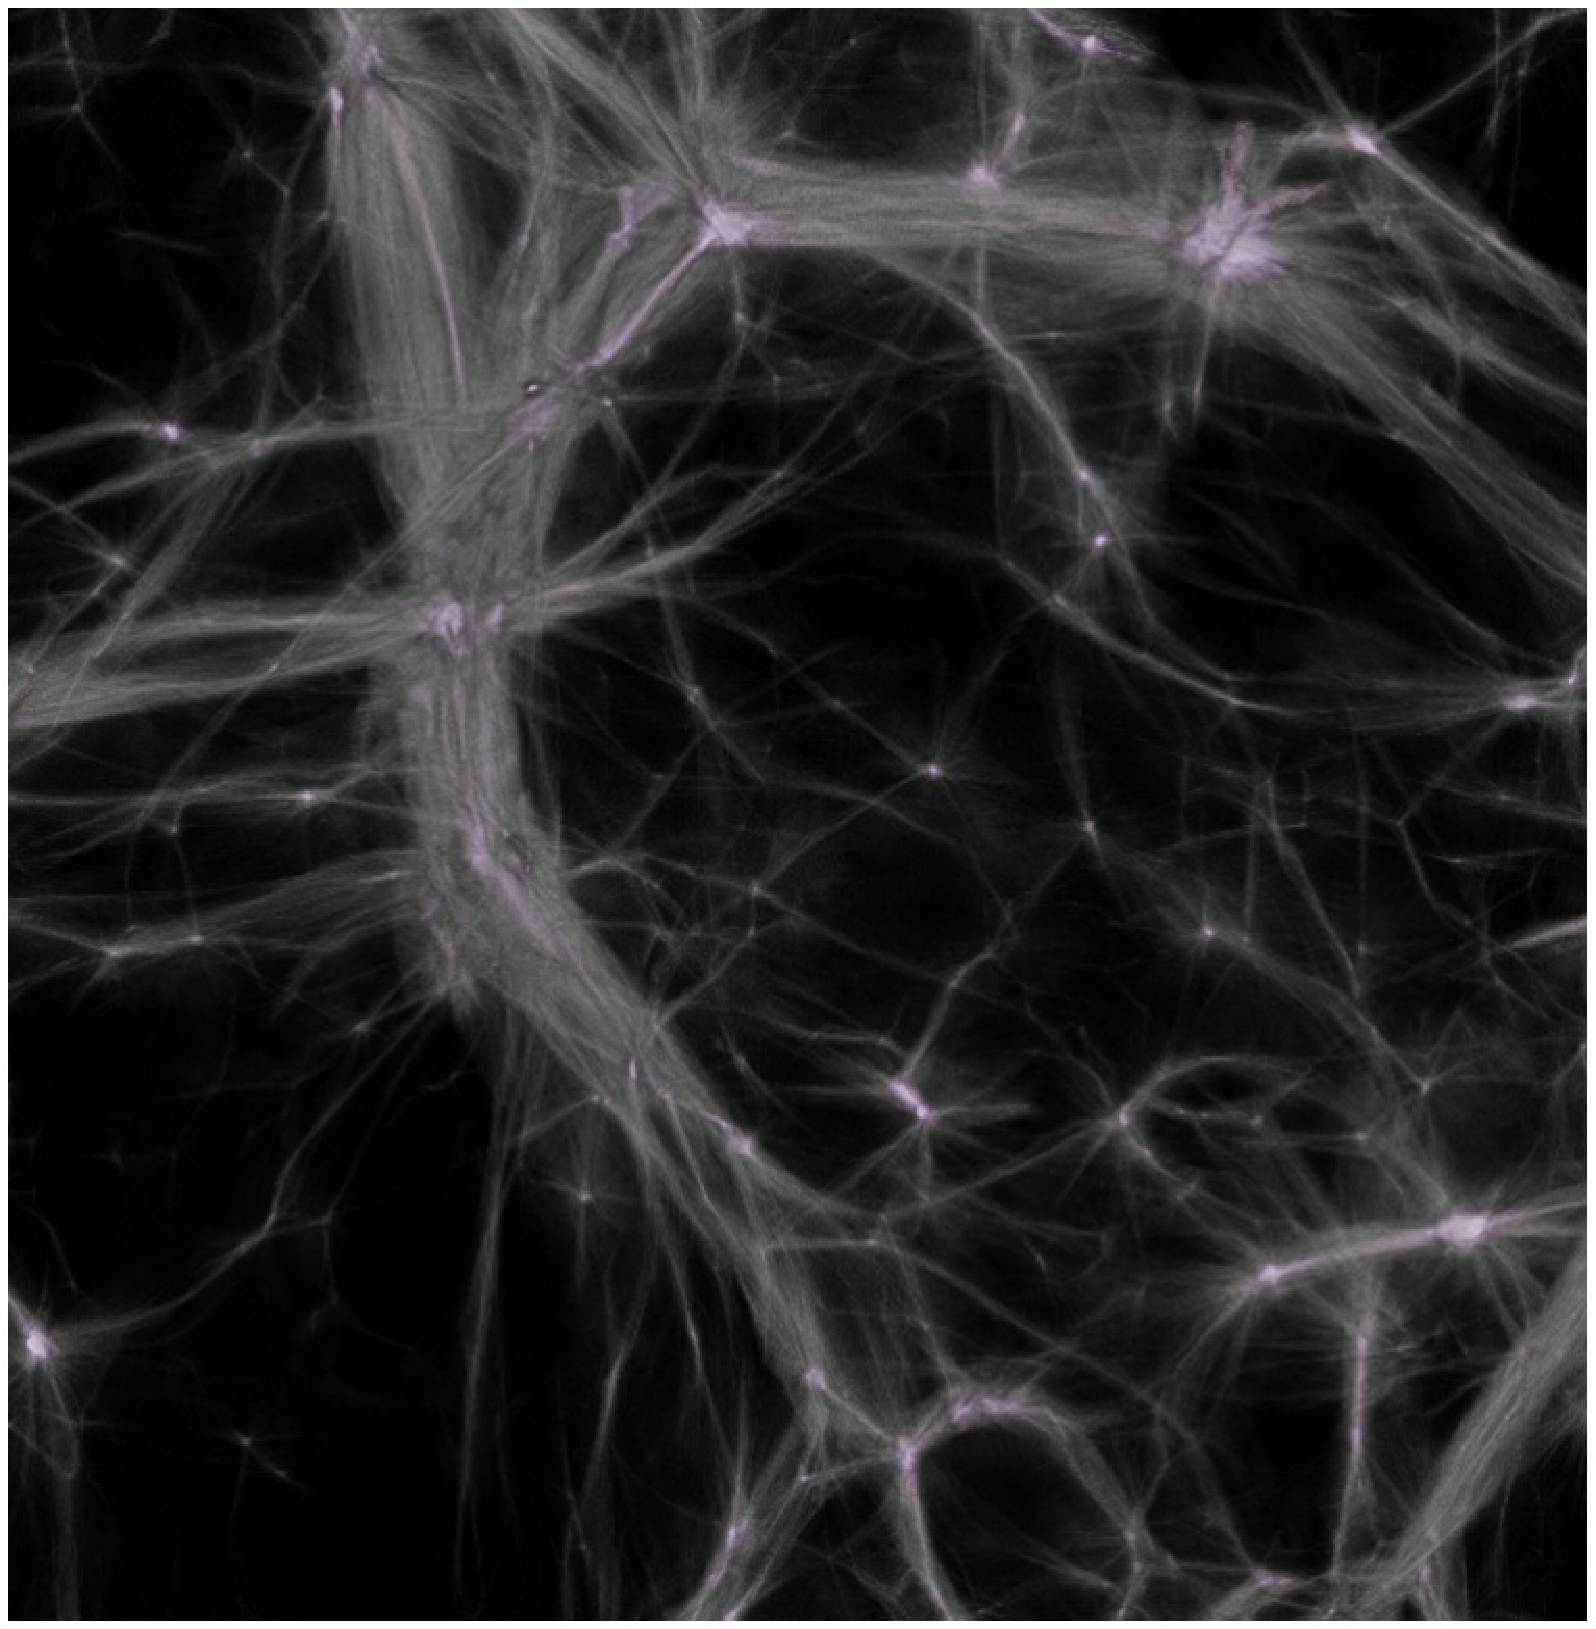
\includegraphics[width=16cm]{Chapter4/Source_v2/fig1.pdf} 
% \caption{3D rendering of the multistream field: the cosmic web structure of a $ 50 h^{-1} \text{Mpc} \times 50 h^{-1} \text{Mpc} \times 50 h^{-1} \text{Mpc}$ slice in a simulation box of side length $100 h^{-1}$ Mpc and $128^3$ particles. The multistream field is calculated at 8 times the native resolution. void(black) is a percolating structure with $n_{str} = 1$. Regions $n_{str} \geq 17$ show a filamentary structure (gray) and the bright spots at the intersections of the filaments are regions with $n_{str} \geq 100$. }
% \label{fig:full}
% \end{figure}

% \bf changed to \bf --- check if it's alright. 
The multistream field objectively characterizes the level of non-linearity in the cosmic web. The `number-of-streams' field or $n_{str}({\bf x})$ is computed from the Lagrangian sub-manifold ${\bf x}({\bf q})$, which is a continuous three-dimensional sheet in a six-dimensional  $({\bf q}, {\bf x})$ space. In this paper, we utilize the tessellation implementation by \cite{Shandarin2012} to calculate the multistream flow field on the GADGET-2 snapshot at $z=0$. This implementation only requires initial and final coordinates of the dark matter particles. 

The $n_{str}(\bf{x})$ values are mostly odd-numbered since each folding in the Lagrangian sub-manifold results in an increase of $n_{str}$ by 2. Exception to this are only at caustics - which have volume measure zero, then the $n_{str}$ is even-valued number. The particles in $n_{str} = 1$ have not experienced orbit crossings and thus these regions are unambiguously identified as void \citep{Shandarin2012}. Foldings in the Lagrangian sub-manifold generally occur one-by-one. For example, a contour of $n_{str} = 7$ will be within a region of $n_{str} \leq 5$. Hence the multistream field commonly has nesting shells, i.e., $ 3 \supseteq  5 \supseteq  7 \supseteq  9 \supseteq  11 \ldots$. Some of the important features of the multistream field are discussed in Appendix \ref{appendix:nstream}.  

The first non-linear DM structures that reach non-perturbative stage of gravitational evolution have $n_{str} = 3$. By visual inspection, these regions generally form a fabric-like open structures that resemble walls. N-body simulations suggest that a DM fluid element after the first 
crossing of a caustic never returns in  a single-streaming state. Therefore the {\it local} condition $n_{str}({\bf r}_{\rm f.e.}) \geq 3$
(where  ${\bf r}_{\rm f.e.}$ is the position of the fluid element) is  sufficient for the fluid element to be bound to the DM web.

All particles that have fallen into a wall will never return to any single-streaming regions, therefore they can be labeled as gravitationally bound to pancakes/walls. The surface contours of higher $n_{str}$ are embedded within the walls. \autoref{fig:full_3d} shows a filamentary structure of the multistream web at $n_{str} \geq 17$. The figure also shows regions around local maxima of the multistream field, usually located at the intersections of filaments.    


The multistream field can be computed at arbitrary resolutions of diagnostic grids. The parameter `refinement factor' denotes the ratio of separation of the particles in Lagrangian grid, $l_l$, to side length of diagnostic grid $l_d$. In a simulation of $128^3$ particles, for instance, multistream field computed on a diagnostic grid of size $256^3$ would have a refinement factor of $l_l/l_d = 2$. 
\begin{comment}
The effects of refinement of the diagnostic grid are discussed in Section \ref{sec:voids} and Section \ref{sub:HaloProperties}. 
\end{comment}

\section{Voids in the multistream field}
\label{sec:voids}

\begin{figure*}
\begin{minipage}[t]{0.99\linewidth}
 \centering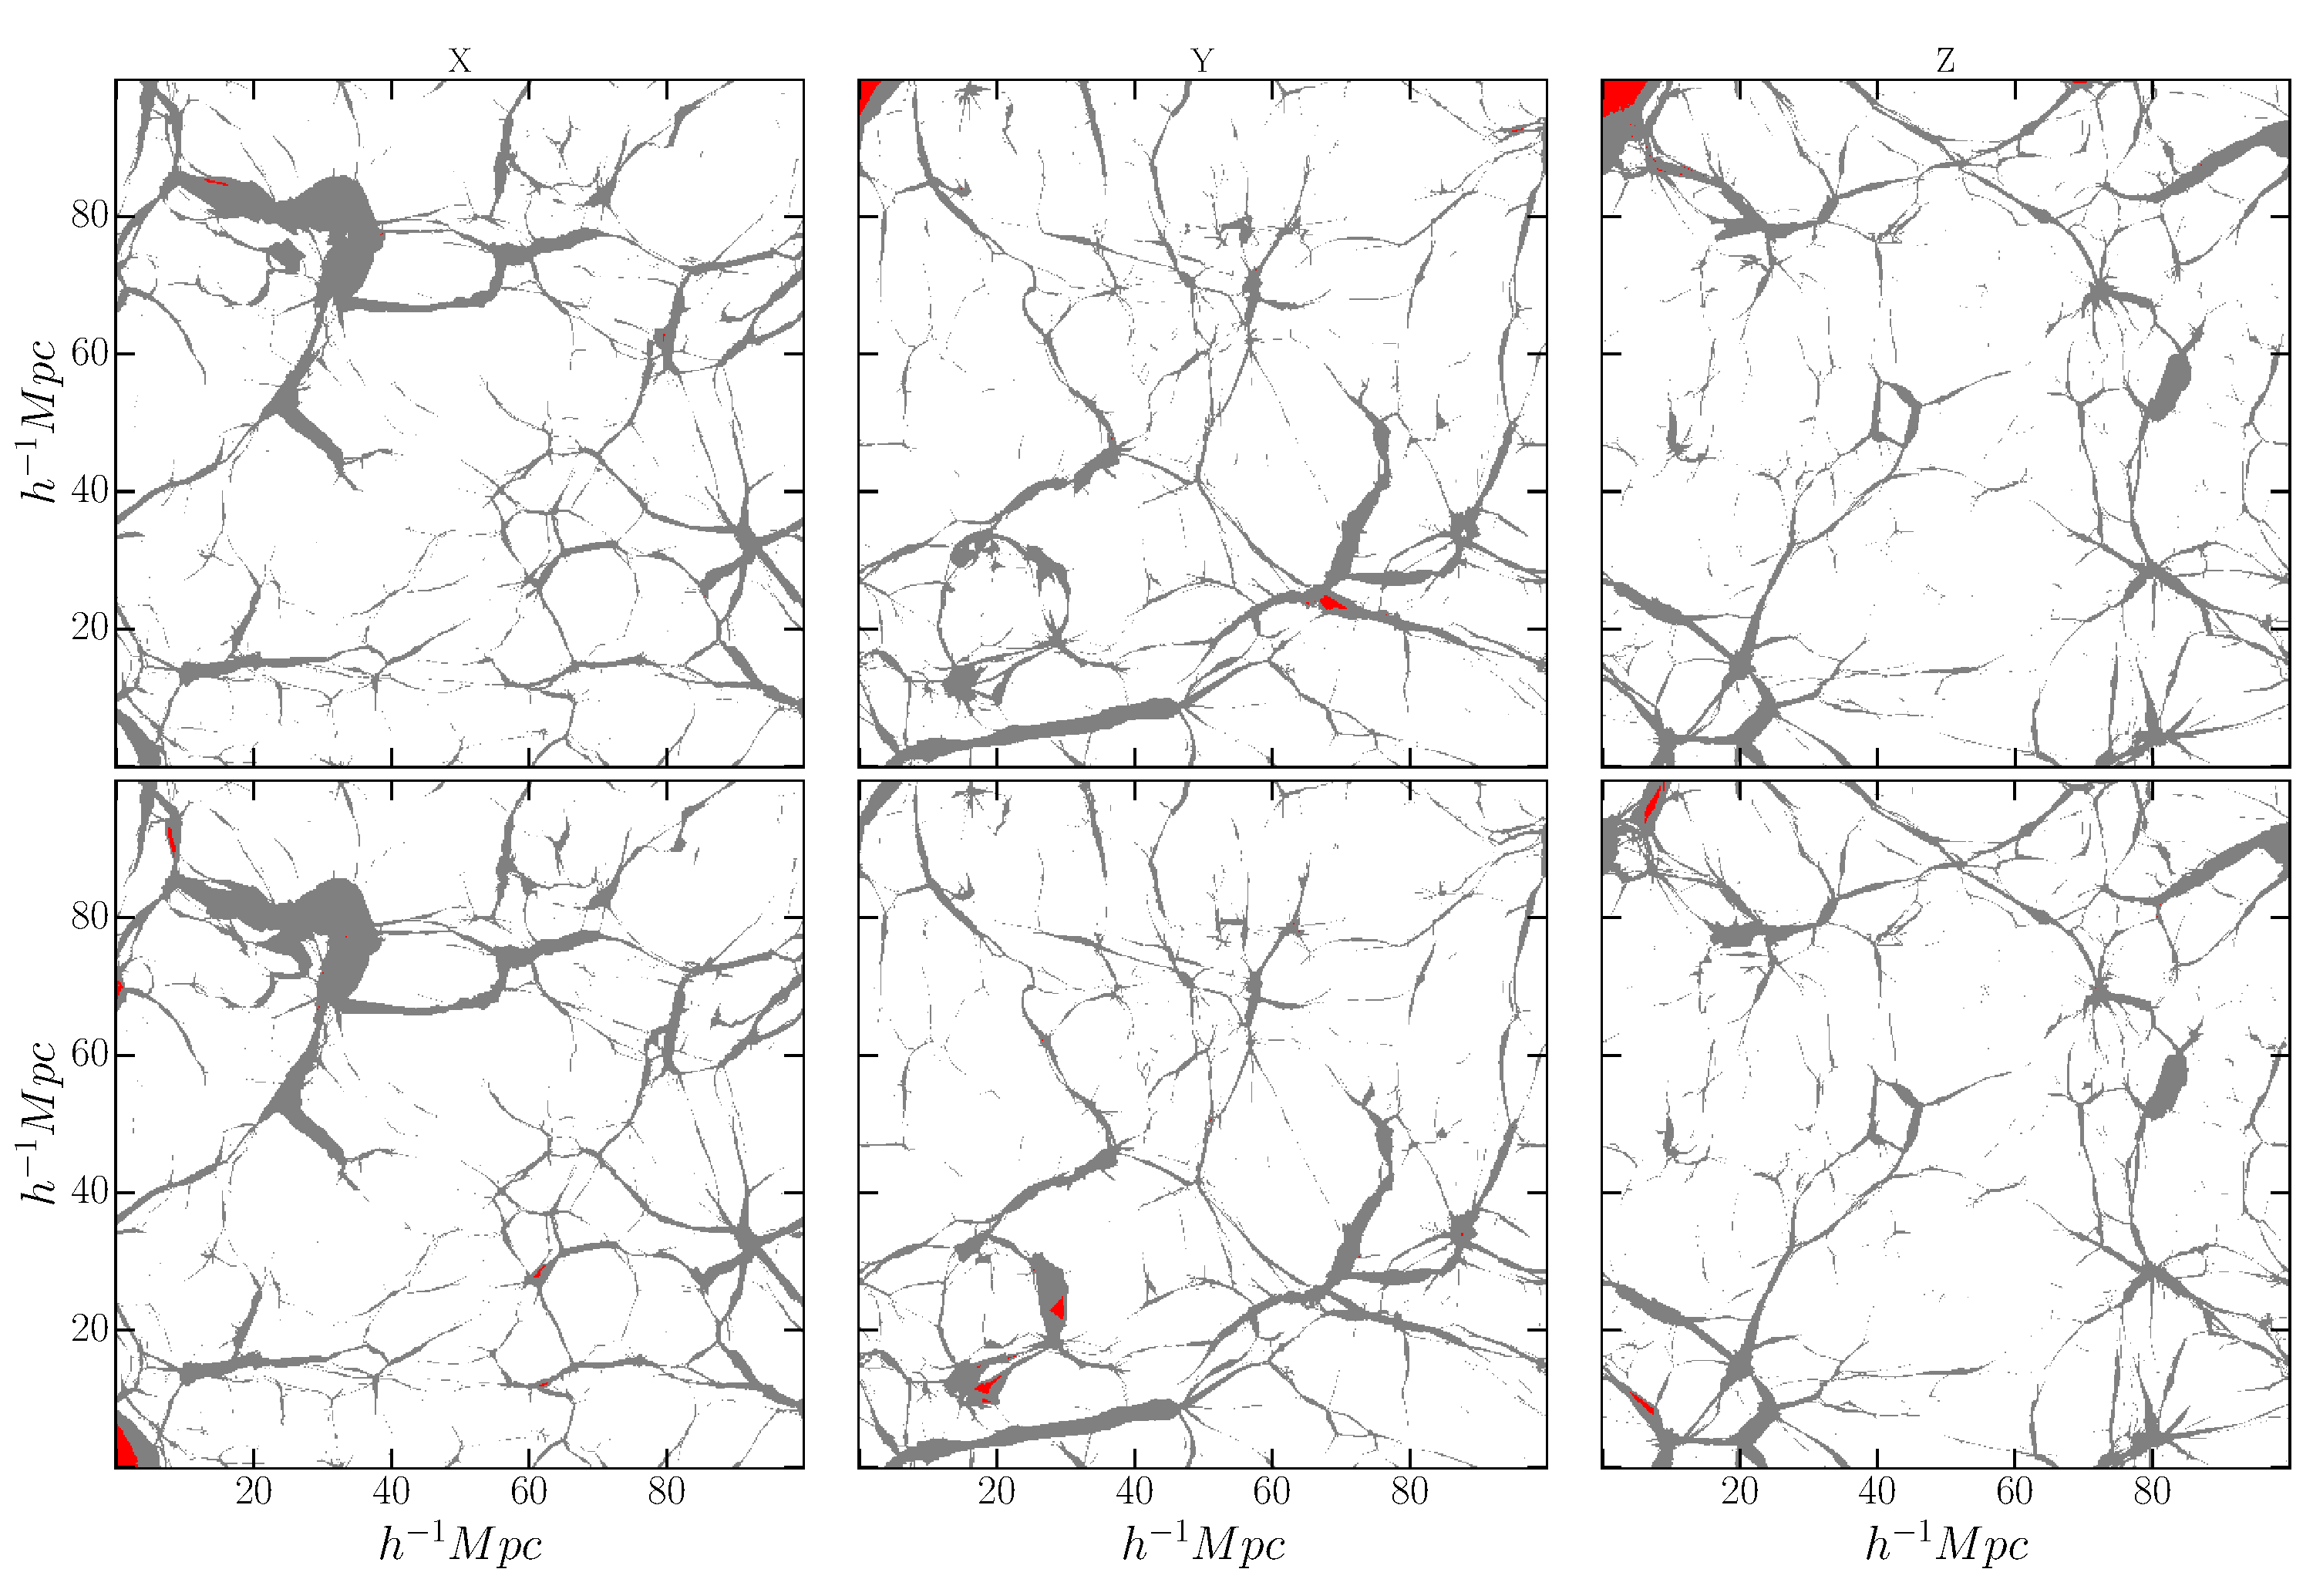
\includegraphics[height=11cm]{Chapter4/Source_v2/fig2.pdf} 
\end{minipage}\hfill
\caption{Opposite faces of the multistream field for the simulation box with $N_p = 128^3$. Non-void regions (gray) have $n_{str} > 1$. The largest void (white) in the entire field spans over the entire box. Rest of the smaller isolated voids (red) occupy very small volume fraction. }
\label{fig:voidFace}
\end{figure*}


Gravitational instability results in movement of the collision-less fluid particles in the Universe from voids to walls, walls to filaments, and filaments to haloes. As we mentioned above in the multistream portrait, the entry of mass particles from single-streaming regions into $n_{str} > 1$ region is irreversible. The converse is obviously not true, that is, the particles in $n_{str} = 1$ regions may move to multistreaming region at a later time in the evolution. At a given cosmic time, sufficient condition for dark matter particles to be bound to non-perturbative and non-linear structures like walls/filaments/haloes is being in multistream regions. Therefore, a single-stream flow implies that gravitationally bound structures haven't yet formed, and thus defined as a void region. This definition of void is unambiguous and physically motivated, as demonstrated by \cite{Shandarin2012}. It is worth stressing that while the density in voids varies, the number-of-streams is uniformly equal to unity.


For simulation box with $128^3$ particles, $n_{str} = 1$ regions have a large volume fraction of $VF_V \approx 93$ per cent regardless of the value of refinement factor (shown in \autoref{tab:VoidStat}). Multi-stream web structure in the simulation with higher mass resolution ($N_p = 256^3$) is better enhanced, and the single streaming void occupies around $90$ per cent of the volume. \autoref{fig:voidFace} shows the single streaming voids occupying large volume of the simulation with $128^3$ particles at refinement factor of 4. 

\begin{table}
\centering
  \caption{Volume fraction $VF_V$ of the voids, total number of isolated voids $N_V$ and the filling fraction of the largest void  $FF_1/VF_V$ at different refinement factors $l_l/l_d$. The filling fractions of the largest void at each refinement factor show that most of the $n_{str} = 1 $ region is almost entirely a single percolating structure.}
\begin{tabular}{|r|r|r|r|r| }
\hline
$N_p$ & $l_l/l_d$ & $VF_V$ & $N_V$ & $FF_1/VF_V$  \\  \hline
$ 128^3$      & $ 1$      & 93.46\%   & 1    & 100\% \\ \hline
$ 128^3$      & $ 2$      & 93.44\%   & 11   & 99.999\% \\ \hline
$ 128^3$      & $ 4$      & 93.44\%   & 113  & 99.999\% \\ \hline
$ 128^3$      & $ 8$      & 93.44\%   & 914  & 99.997\% \\ \hline
$ 256^3$      & $ 1$      & 90.80\%   & 11   & 99.999\% \\ \hline
$ 256^3$      & $ 2$      & 90.80\%   & 97   & 99.999\% \\ \hline
$ 256^3$      & $ 4$      & 90.80\%   & 1029 & 99.997\% \\ \hline
$ 256^3$      & $ 8$      & 90.80\%   & 7259 & 99.964\% \\ \hline

\end{tabular}
\label{tab:VoidStat}
\end{table}



\subsection{Connectivity of the voids}
\label{sec:voidPerc}




In order to find whether the void regions of the multistream field are connected or not, we isolate three-dimensional segments with $n_{str} = 1$ and separately label them. The number of disconnected voids in the simulation with $N_p = 128^3$ range from 1 (for refinement factor, $l_l/l_d =  1$) to about $900$ (for $l_l/l_d= 8$) as shown in \autoref{tab:VoidStat}. Number of isolated voids increases similarly in the simulation with $N_p = 256^3$ particles as well. 

Smoothing of the structure at lower resolution of the multistream field results in increased connectivity of single-streaming regions. In \autoref{fig:voidFace}, opposite faces on each axes of the multi-field, show a large connected void (white). This means that the largest void percolated throughout the multistream field in all directions. This result is in agreement with \cite{Falck2015}, who studied percolation of ORIGAMI-voids in simulations with side lengths of $100$ and $200  h^{-1} \text{Mpc}$. In addition to the percolating the field, the largest void also fills most of the void volume: the ratio of filling fraction of the largest void $FF_1$ to the volume fraction of $n_{str} = 1$ regions in the simulation is close to unity (see \autoref{tab:VoidStat}). This phenomenon is seen at each of the refinement factors in our analysis. Hence, over $99.9$ per cent of the single-streaming sites are connected throughout the simulation box, and they form a single empty region.  
    

As previously mentioned, the multistream web structures of $n_{str} = 3$ form the first gravitationally collapsed structures. These tiny structures are better resolved in higher refinement factors, and they tend to enclose greater number of pockets of single-streaming voids inside them. The red regions in \autoref{fig:voidFace} some of the small voids on faces of the simulation box with $128^3$ particles. Despite increase in the number of small voids at each of the refinement factors, these void regions (i.e., the single streaming regions excluding the largest void) collectively occupy less than $0.1$ per cent of the total void volume in both the simulations. It is also likely that the small voids are simply due to numerical noise. However, the major conclusion regarding small voids remains the same up to refinement factor of 8. We do not pursue further investigation due to tiny effects.  

 
\subsection{Halo boundaries within the void}
\label{sec:voidHaloes}

\begin{figure}
\begin{minipage}[t]{.99\linewidth}
\centering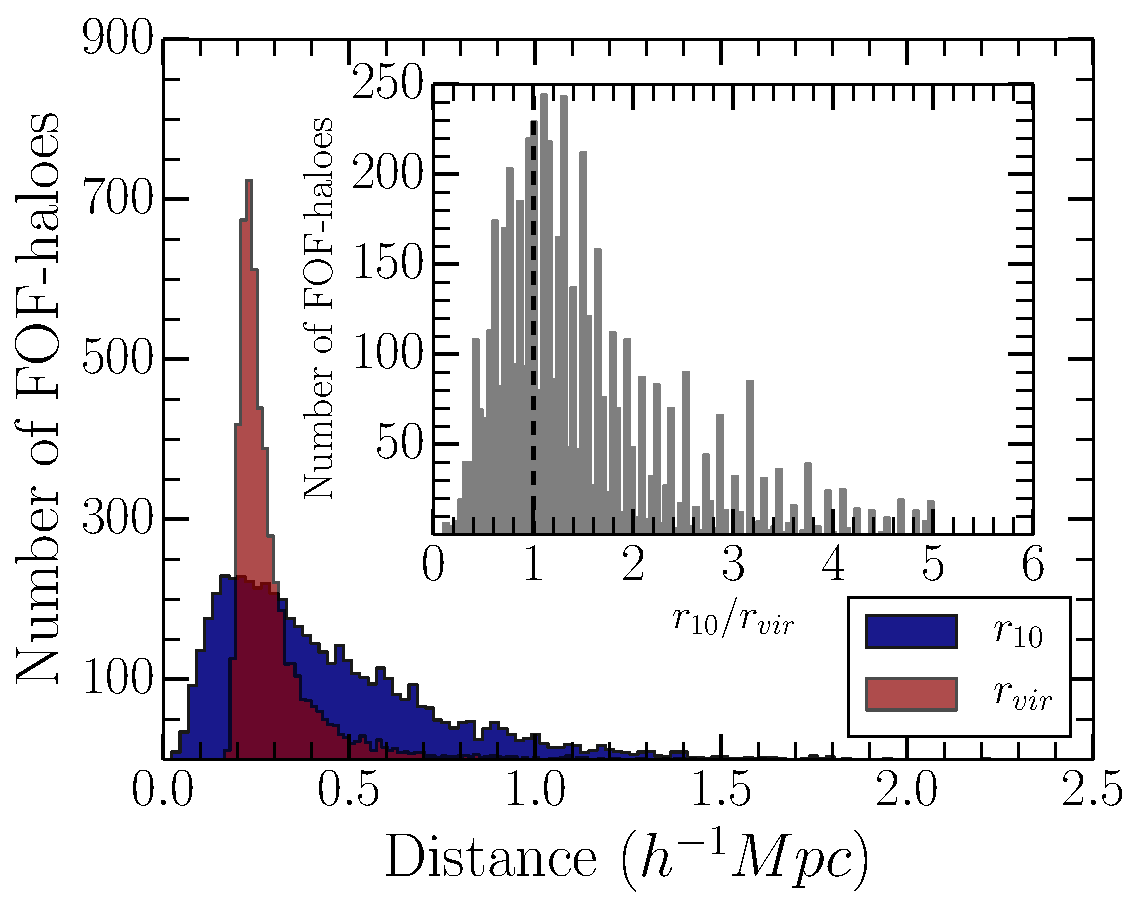
\includegraphics[width=10.cm]{Chapter4/Source_v2/fig3.pdf} 
\end{minipage}\hfill
\caption{Single-streaming void distribution on diagnostic spheres around FOF-haloes are considered. At radius $r_{10}$, each diagnostic sphere has $n_{str} = 1$ on 10 per cent of its spherical surface. Distribution function of $r_{10}$ (blue) and FOF-radii $r_{vir}$ (red) are shown. Inner plot shows the distribution function of $r_{10}/r_{vir}$. The haloes within the dashed line have at least 10 per cent of their virial-surfaces in contact with $n_{str} = 1$ regions.}
\label{fig:Vfr_all}
\end{figure}


Dark matter haloes are the most non-linear objects in the cosmic web. With the exception of ORIGAMI \citep{Falck2012}, most of the halo finders do not consider multistreaming in the configuration space for finding haloes. Potential haloes found by several such halo finding methods, hence, may have boundaries that intersect with the single-streaming void, which is the least non-linear structure in the dark matter universe. \cite{Colberg2008} even mention existence of `void-haloes' in several halo finder algorithms.  

We studied the $n_{str}$ environment of the haloes detected using the Friends-of-Friends method (FOF-\citealt{Davis1985}) as illustrated in \autoref{fig:Vfr_all}. FOF-haloes with more than 20 particles are detected using linking-length of $b=0.2$ in the simulation with $128^3$ particles. We implement the diagnosis method prescribed in \cite{Ramachandra2015}: a large number of points are randomly selected on diagnostic spherical surfaces centred at the FOF-centre of the halo. Multi-stream values are iteratively calculated at these spherical surfaces of various radii. We define the distance from centre of a halo, $r_{10}$, where $n_{str} = 1$ at 10 per cent of the surface of the diagnostic sphere. Distribution of this void-distance parameter is compared to the virial radii $r_{vir}$ of the FOF-haloes. Surprisingly, $r_{10}$ distribution peaks at slightly lower values than the $r_{vir}$ distribution. This implies a large number of FOF-haloes are in the vicinity of the void. 

For specific examples of some FOF-haloes, \cite{Ramachandra2015} showed that single-stream may appear within their virial radii too. The distribution of $r_{10}/r_{vir}$ in the inner plot of \autoref{fig:Vfr_all} shows the same phenomenon. The FOF-haloes within $r_{10}/r_{vir} < 1$ (represented by the vertical dashed line) have $n_{str} = 1$ on 10 per cent of their virial surfaces. The figure illustrates that a large number of FOF-haloes satisfy this condition, thus are in contact with the void surfaces. Hence not all the FOF particles have undergone a gravitational collapse during their evolution. 


For methods such as FOF, there is no unambiguous linking-length criterion for voids. Similarly for the density fields, a range of under-densities are prescribed by various void finder methods (cf. \citealt{Colberg2008}). On the other hand, the multistream field unambiguously identifies all the regions without a single gravitational collapse as voids. Haloes detected on the multistream field may address the issue of haloes being in contact with voids. 
\begin{comment}
In the halo finding framework in Section \ref{sec:haloDetection}, we explicitly make sure that haloes are not in contact with the void at their boundaries. 
\end{comment}

\section{Percolation in the multistream web}
\label{sec:percolation}
%\hl{[Section 6 from previous version moved here. Section 5 and 6.1 reserved for the 2nd paper]}

\begin{figure}
\begin{minipage}[t]{.99\linewidth}
  \centering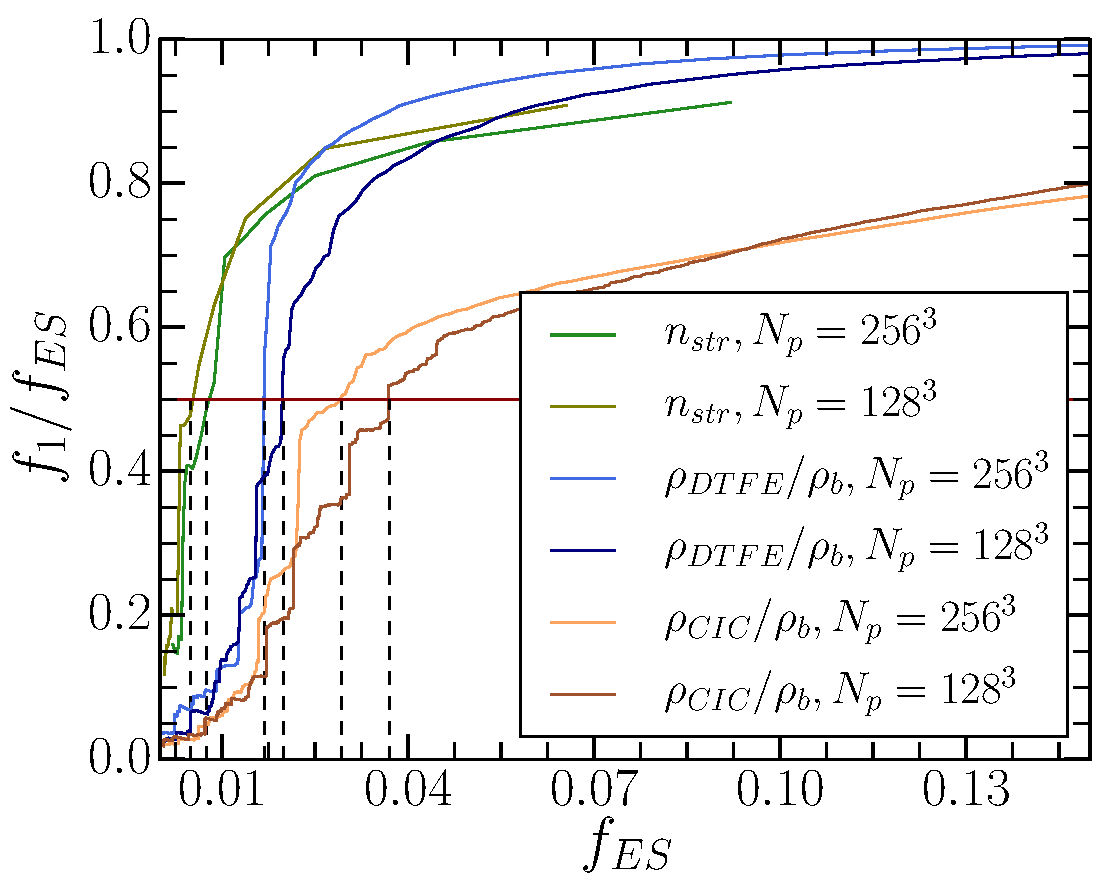
\includegraphics[width=10.cm]{Chapter4/Source_v2/fig4.pdf} 
\end{minipage}\hfill
\caption{Percolation plot in the multistream field and mass density. Two density estimators - CIC and DTFE are shown. Percolation transition (at $f_1/f_{ES} = 0.5$ shown by the horizontal red line) occurs at smaller excursion set volumes for the multistream field, as seen by the dashed lines for both the curves. It is worth stressing that the percolation curves for $n_{str}$ field are bounded by conditions $f_{ES} < 0.1$. }
\label{fig:PercTh}
\end{figure}

\begin{figure*}
\begin{minipage}[t]{.99\linewidth}
  \centering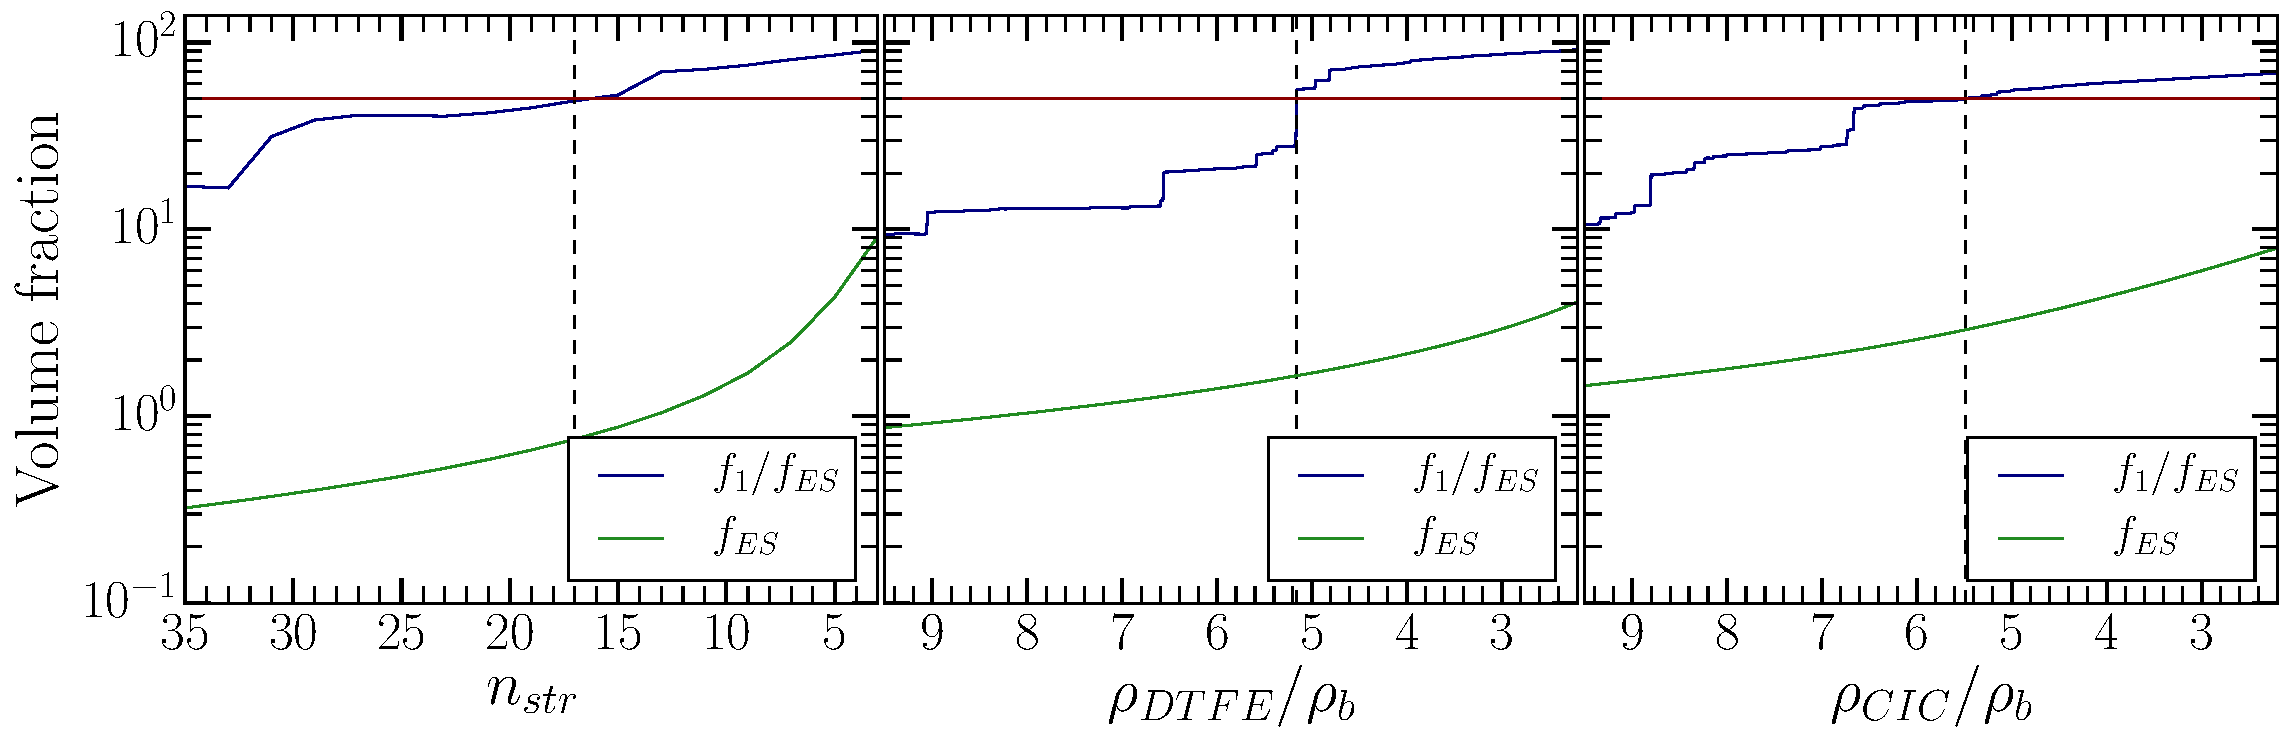
\includegraphics[height=5.7cm]{Chapter4/Source_v2/fig5.pdf} 
\end{minipage}\hfill
\caption{Percolation threshold in the multistream (left panel) and matter density fields. Matter density is calculated using DTFE (middle panel) and CIC (right panel) with a refinement factor of 2 in the simulation with $256^3$ particles. The volume fraction of excursion set and the filling fraction of the largest structure is shown. Percolation transition in multistream field at $n_{str} = 17$ is shows by the dashed vertical line. Percolation at $\rho_{DTFE}/ \rho_b = 5.16 $ and $\rho_{CIC}/ \rho_b = 5.49 $ are shown by the dashed vertical line. }
\label{fig:HaloFil}
\end{figure*}

A single percolating void fills the $n_{str} = 1$ regions almost entirely, as discussed in Section \ref{sec:voidPerc}. Disconnected pockets of void may exist, but they collectively occupy very small volume fraction (less than 0.1 per cent of the total volume as tabulated in \autoref{tab:VoidStat}). Whereas, the non-void structure in the multistream field has a different topological structure. The regions selected with a lower bound on $n_{str}$ could be isolated (generally for high $n_{str}$ thresholds) or connected in a percolating region (for low $n_{str}$ thresholds). We investigate the topological transitions in these excursion sets of multistream field. 



The volume fraction as a function of number-of-streams decreases according to a power law in the $n_{str} > 1$ structure (\citealt{Shandarin2012} and \citealt{Ramachandra2015} report $\text{VF}(n_{str})$ decreasing as ${n_{str}}^{-2.8} $ and  ${n_{str}}^{-2.5}$ respectively for their simulations). The volume fraction of the excursion set $f_{ES}(n_i)$ is the ratio of volume of all the regions with a lower bound $n_i$ on the multistream field to the total volume $V_{tot}$ of the simulation box, i.e, $ \displaystyle f_{ES}(n_i) = \frac{V_{ES}}{V_{tot}} =  {\sum\limits_{n_{str} \geq n_i} \text{VF} ({n_{str}})}$. Since volume fraction of the each $n_{str}$ rapidly increases with an decrease in multistream value, so does the $f_{ES}$. 


The excursion set may have number of isolated segments of different volumes. A measure of connectivity in the excursion set regions can be given by the filling fraction, $f_1/f_{ES}$, where $f_1$ is the volume fraction of the largest isolated region in the excursion set. $f_1$ can be computed numerically in the simulations. If the value of $f_1/f_{ES}$ is close to 0, then none of the isolated regions dominate the excursion set. This implies absence of percolation. If $f_1/f_{ES}$ is close to one, it implies a single connected structure dominates most of the excursion set. 


The filling fraction $f_1/f_{ES}$ grows from 0 to 1 occurs rapidly $f_{ES}$ during percolation phase transition. A practical robust definition of the percolation transition is at $f_1/f_{ES} = 0.5$, i.e, when the  largest region occupies more than 50 per cent of the excursion set volume. The percolation plot in \autoref{fig:PercTh} reveals this phenomenon. Excursion volume fraction $f_{ES}$ at this transition, $f_{ES}^{(p)} = 0.48$ and $0.75$ per cent for the simulations with with $128^3$ and $256^3$ particles respectively (although the numbers were obtained in one simulation each. The difference may be well within the range of statistical errors for this size of simulation box). After the percolation transition, the filling fraction of the largest structure stabilizes towards unity. 


The nature of the transition in mass density field is similar to that in multistream field. For the simulation simulation with $256^3$ particles, the density is calculated using CIC method at $256^3$ and $512^3$ grid points. In \autoref{fig:PercTh}, the percolation phenomenon in both mass density fields is shown along with that of multistream fields. The excursion set volume fraction at percolation transition, $f_{ES}^{(p)}$ is lower for multistream field, because the filaments in the multistream field are thinner than that of density picture. Volume fraction of the largest structure detected in the density field also tends to unity with decreasing $f_{ES}$, albeit less rapidly as that of the multistream field. This means that while the largest structure in a multistream web occupies most of the structure, the over-density excursion set is more fragmented.
  







The excursion volume fraction of the multistream web structure is limited to a small fraction of  less than 10 per cent since rest of the volume is void. The excursion set volume fraction increases with decreasing number-of-streams and reaches it's maximum at $n_{str} = 3$.  At this limit the filling fraction $f_1/f_{ES}$ is still less than unity, about 95 per cent. These two peculiar properties of the multistream field explain the shape of the percolation curves in \autoref{fig:PercTh}.
Since the multistream flow field is a discrete data field, the percolation transition is seen to occurs at a particular value of $n_{str}$ rather than a large range of values. For $n_{str} = 17$, the largest structure in the excursion set occupies more than half the volume of the entire excursion set. At this multistream threshold, the largest segment starts spanning large volume of the simulation box (as observed in the left panel of \autoref{fig:HaloFil}). The volume fraction of the excursion set at this percolation transition is $f_{ES}^{(p)} = 0.75$ per cent for simulation with $256^3$ particles. 

The percolation transition at $n_{str} = 17$ could be used as a criterion for detecting filaments in the cosmic web. Since the largest $n_{str} \geq 17$ region occupies more than 50 per cent of the excursion set, it is essentially the `backbone' of the cosmic web \citep{Shandarin2010b}. Heuristic analysis as discussed by \cite{Ramachandra2015} also arrived at the same threshold for identifying filaments. That analysis was based on a multistreams variation in halo environments, hence a local value. From our percolation analysis, we see that it is also justified globally. 



\begin{comment}
\begin{figure}
\begin{minipage}[t]{.99\linewidth}
  \centering\includegraphics[width=10.cm]{fig5n.pdf} 
\end{minipage}\hfill
\caption{Percolation threshold in the multistream field with refinement factor of 2 in the simulation with $256^3$ particles. The volume fraction of excursion set and the filling fraction of the largest structure is shown. Percolation transition at $n_{str} = 17$ is shows by the dashed vertical line. }
\label{fig:HaloFilDen}
\end{figure}

\begin{figure}
\begin{minipage}[t]{.99\linewidth}
  \centering\includegraphics[width=10.cm]{fig6n.pdf} 
\end{minipage}\hfill
\caption{Percolation threshold in the density field of the simulation with $256^3$ particles calculated from the CIC method. The volume fraction of excursion set and the filling fraction of the largest structure is shown. Percolation at $\rho/ \rho_b = 4.8 $ is shown by the dashed vertical line.}
\label{fig:HaloFilNst}
\end{figure}

\end{comment}


In the simulation with $256^3$ particles, percolations in the density field occurs at $\rho_{DTFE}/ \rho_b = 5.16 $ and $\rho_{CIC}/ \rho_b = 5.49 $ for densities calculated with DTFE and CIC respectively. Here $\rho_b = 256^3 / 100^3 M_{\odot} h^{-3} \text{Mpc}^{-3}$, the background density. Notice that these values correspond to the density as calculated by the CIC and DTFE algorithms, and it might be different for other density finding methods. The volume fraction of the excursion set of over-densities at the percolation, $f_{ES}^{(p)} = 2.7$ per cent, is considerably higher than the corresponding $f_{ES}^{(p)}$ value in the multistream field. This implies that the percolation occurs at larger values of filling fraction in mass densities. 


%\hl{CHECK values again, Previous: $\rho/ \rho_b = 4.8 $ and $f_{ES}^{(p)} = 2.7$}


\section{Local geometry of the multistream field}
\label{sec:hessian}
\begin{figure}
\begin{minipage}[t]{.99\linewidth}
  \centering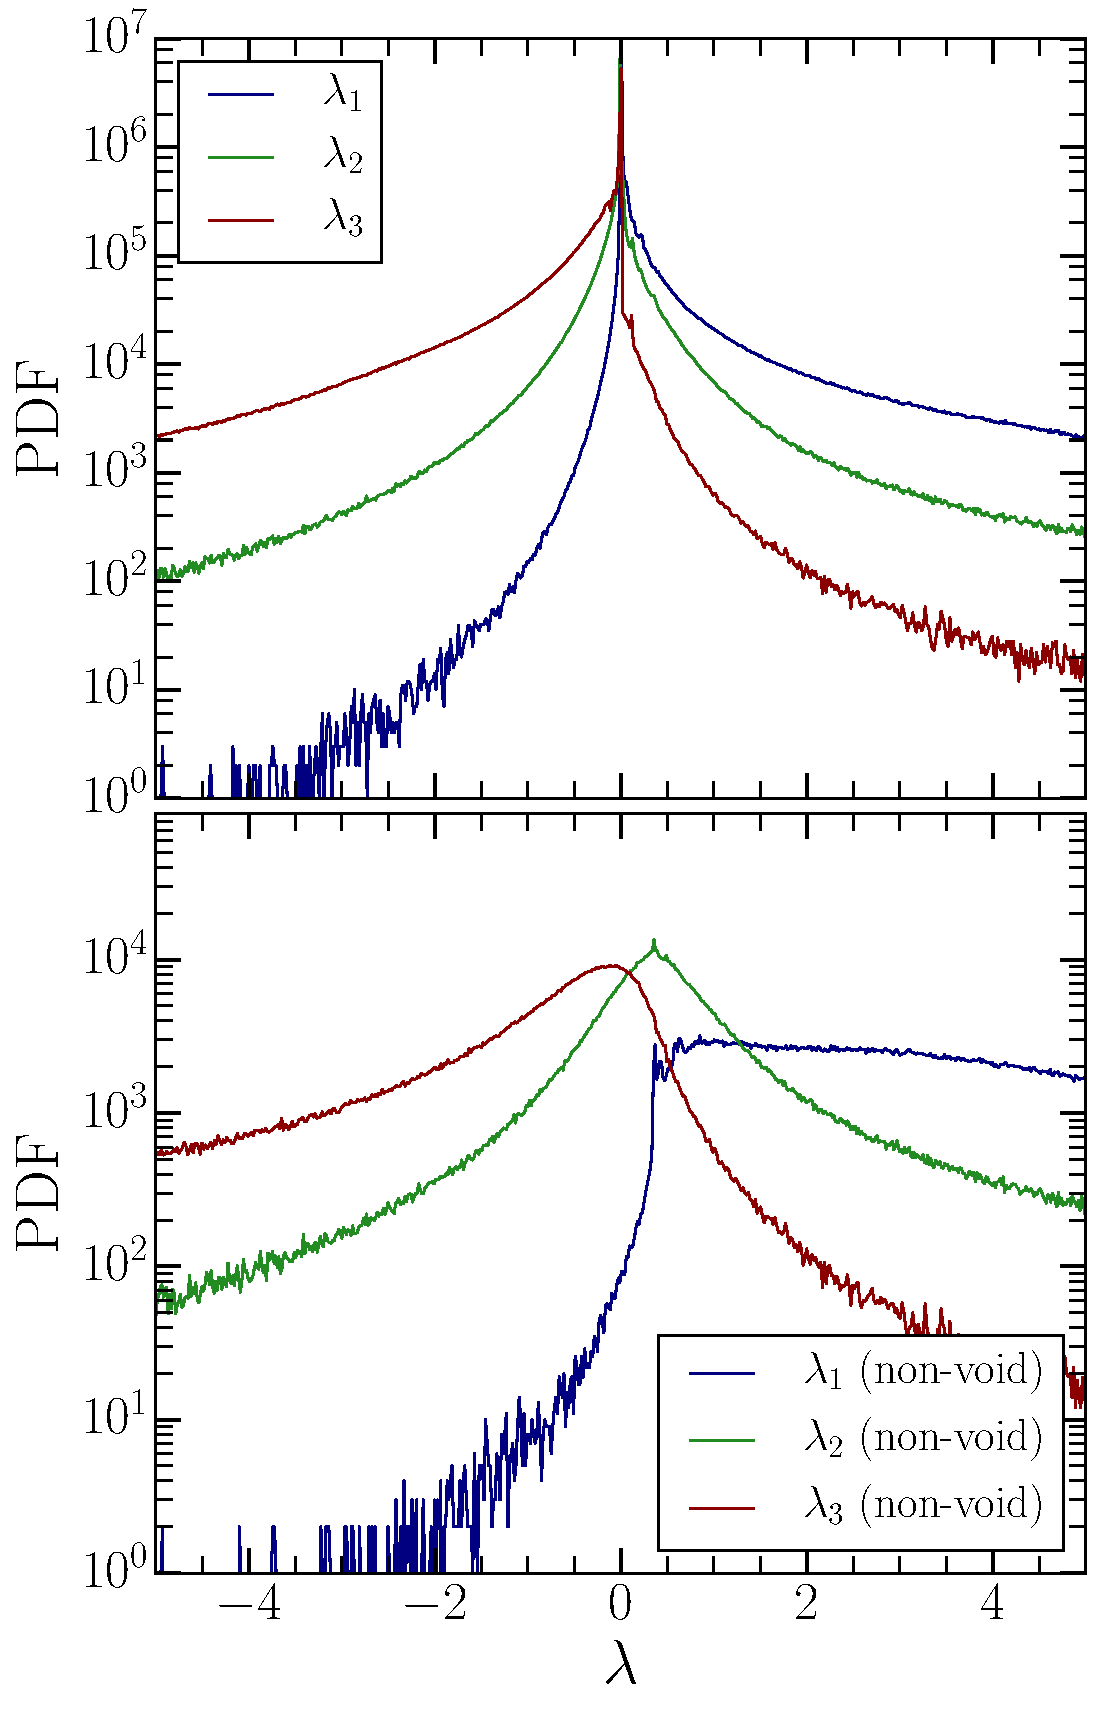
\includegraphics[width=10.cm]{Chapter4/Source_v2/fig6.pdf} 

\end{minipage}\hfill
\caption{Probability distribution function of the sorted eigenvalues of the Hessian ${\bf H}(-n_{str})$ in the simulation box with $N_p = 128^3$. Top panel: Distribution in the entire simulation box. The multistream field is calculated at refinement factor $l_l/l_d= 2$ and smoothing scale of equal to $l_d$. All the three eigenvalue data fields have a highest number of points where their value is 0. Bottom panel: Hessian eigenvalues for the non-void region ($n_{str} > 1$) is shown. Total number of eigenvalue triplets are less than $10$ per cent of that of the full simulation box. Eigenvalues close to zero in non-void regions are notably fewer than in the entire simulation box.}
\label{fig:lambdasPDF}
\end{figure}


\begin{figure}
\begin{minipage}[t]{.99\linewidth}
  \centering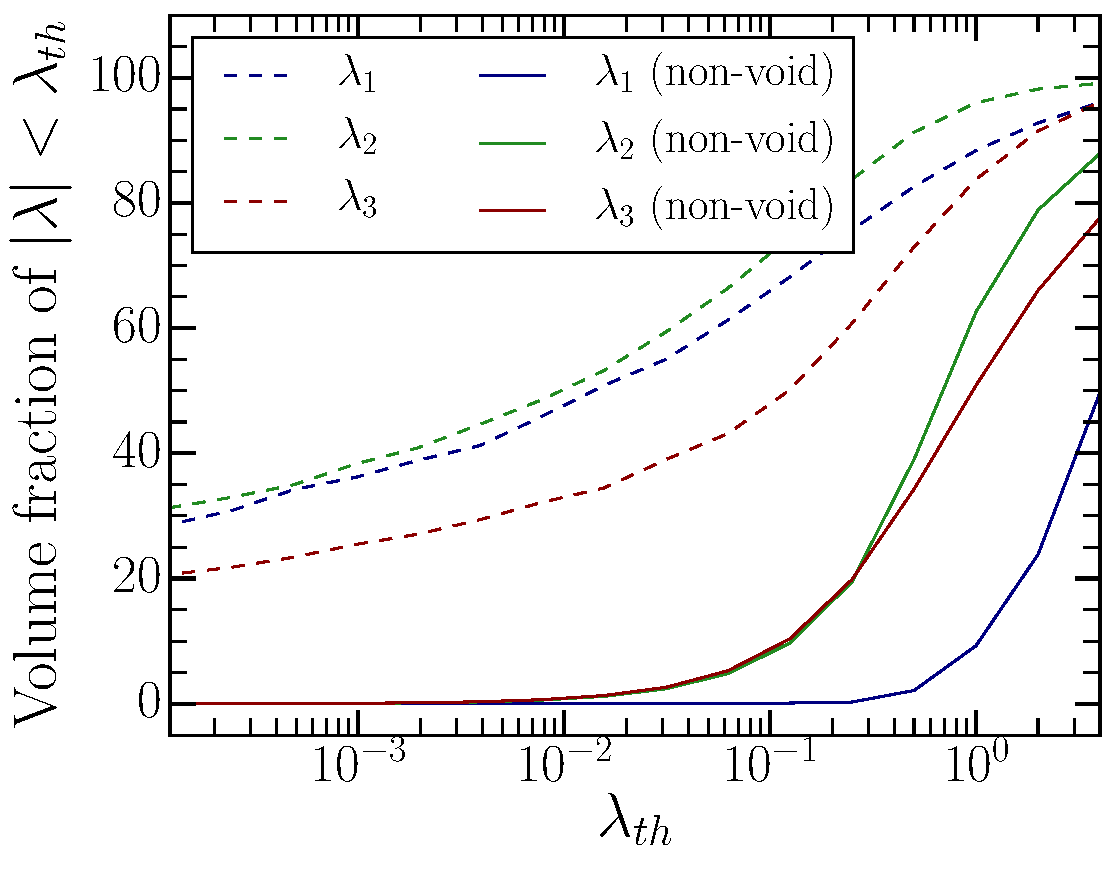
\includegraphics[width=10.cm]{Chapter4/Source_v2/fig7.pdf} 

\end{minipage}\hfill
\caption{Comparison between small eigenvalues of the multistream Hessian ${\bf H}(-n_{str})$. Percentage of eigenvalues with absolute values less than a cut-off, $\lambda_{th}$ are shown for full simulation box (dashed lines) and the multistream web structure (solid lines). The multistream web has fewer eigenvalues below $\lambda_{th} = 0.1$. The void seems to have most of the small eigenvalues. } 
\label{fig:lambdasSmall}
\end{figure}


The multistream field has a constant value of $1$ for around $90$ per cent of the simulation box. At least one gravitational collapse occurs in the remaining $10$ per cent of the volume. In these non-void regions, the $n_{str}$ value varies from 3 to very high values, often in the order of thousands. In the multistream field of refinement factor of 2 for simulation with $N_p = 128^3$ particles, maximum $n_{str}$ is 2831. Within the non-void structure, the multistream field may have several local maxima, minima and saddles. Variation of $n_{str}$ is especially high inside halo boundaries, where the particles in their non-linear stage of evolution have undergone a large number of flip-flops.  

Local second order variation in a scalar field $f$ like the multistream field can by found using the Hessian matrix ${\bf H}(f)$. An element of the Hessian matrix is given in \autoref{eq:Hess}, where $i$ and $j$ can be any of $x$, $y$ or $z$ directions.  

\begin{equation}
\label{eq:Hess}
 {\bf H}_{ij}(f) = \frac{\partial^2 f}{\partial x_i \partial x_j} 
\end{equation}

In our analysis, we have chosen $f = -n_{str}(\bf{x})$ for understanding local variations of the multistream field. The resulting Hessians at each point on the configuration space are always symmetric matrices, as illustrated in Appendix \ref{appendix:Eigen}. The eigenvalues of these Hessian matrices are always real, and depending on if their values are positive or negative, one may infer local geometrical features in the multistream field. 
\begin{comment}
We utilise a framework based on Hessian eigenvalues in smoothed multistream field for the detection of haloes.   
\end{comment}




Within the void, there is no variation in the multistream values. Hessians ${\bf H}(-n_{str})$ are zero matrices in large volume fraction of the simulation box (around 90 per cent in both the simulations) due to the constant value of $n_{str} = 1$ in this percolating void. Eigenvalues of these Hessian matrices, sorted as $ \lambda_1 \geq \lambda_2 \geq \lambda_3 $ are close to 0 at a large number of regions as shown in the top panel of \autoref{fig:lambdasPDF}. In the simulation with $128^3$ particles, the median values of each eigenvalue are $0.09$, $-3\times 10^{-10}$ and $-0.11$ for  $\lambda_1$, $\lambda_2$ and $\lambda_3$ respectively. By selecting just the non-void region by $n_{str} > 1$, notably fewer number of eigenvalues have small absolute values. The median values of each of the eigenvalues in the non-void regions are $4.01$, $0.48$, and $-0.85$ respectively for $\lambda_1$, $\lambda_2$ and  $\lambda_3$. Bottom panel in \autoref{fig:lambdasPDF} shows a significant change in the probability distribution of Hessian eigenvalues around 0, the distribution pattern at the tails are mostly identical to the distribution pattern in the entire simulation box. 


A large fraction of eigenvalues in non-void regions are still around 0, but their percentage is quite less compared to that of the entire box. For instance, nearly 66 per cent of $\lambda_1$'s, 72 per cent of $\lambda_2$'s and 48 per cent of $\lambda_3$'s are  within in the range of $0.0 \pm 0.1$ in the entire simulation box. However, with the exclusion of void regions, these volume fractions drops to 0.1, 7.7 and 8.4 per cent respectively (\autoref{fig:lambdasSmall}). Hence most of the eigenvalues at the void region have small absolute values.

Hessian eigenvalues in multistream fields differ from that in density, gravitational potential or velocity shear tensor. Constant scalar value of $n_{str}$ facilitates the Hessian ${\bf H}(-n_{str})$ matrices to be presumptively close to zero. On the other hand, in density field manifests in a range of low values in the voids, resulting in non-zero Hessian matrices. Eigenvalues of velocity shear tensor do not peak at zero either \cite{Libeskind2013}. For the deformation tensor, morphological characterization of the cosmic web using Zel'dovich formalism shows that each eigenvalue must be negative in voids. 

\begin{figure*}
\begin{minipage}[t]{0.99\linewidth}
 \centering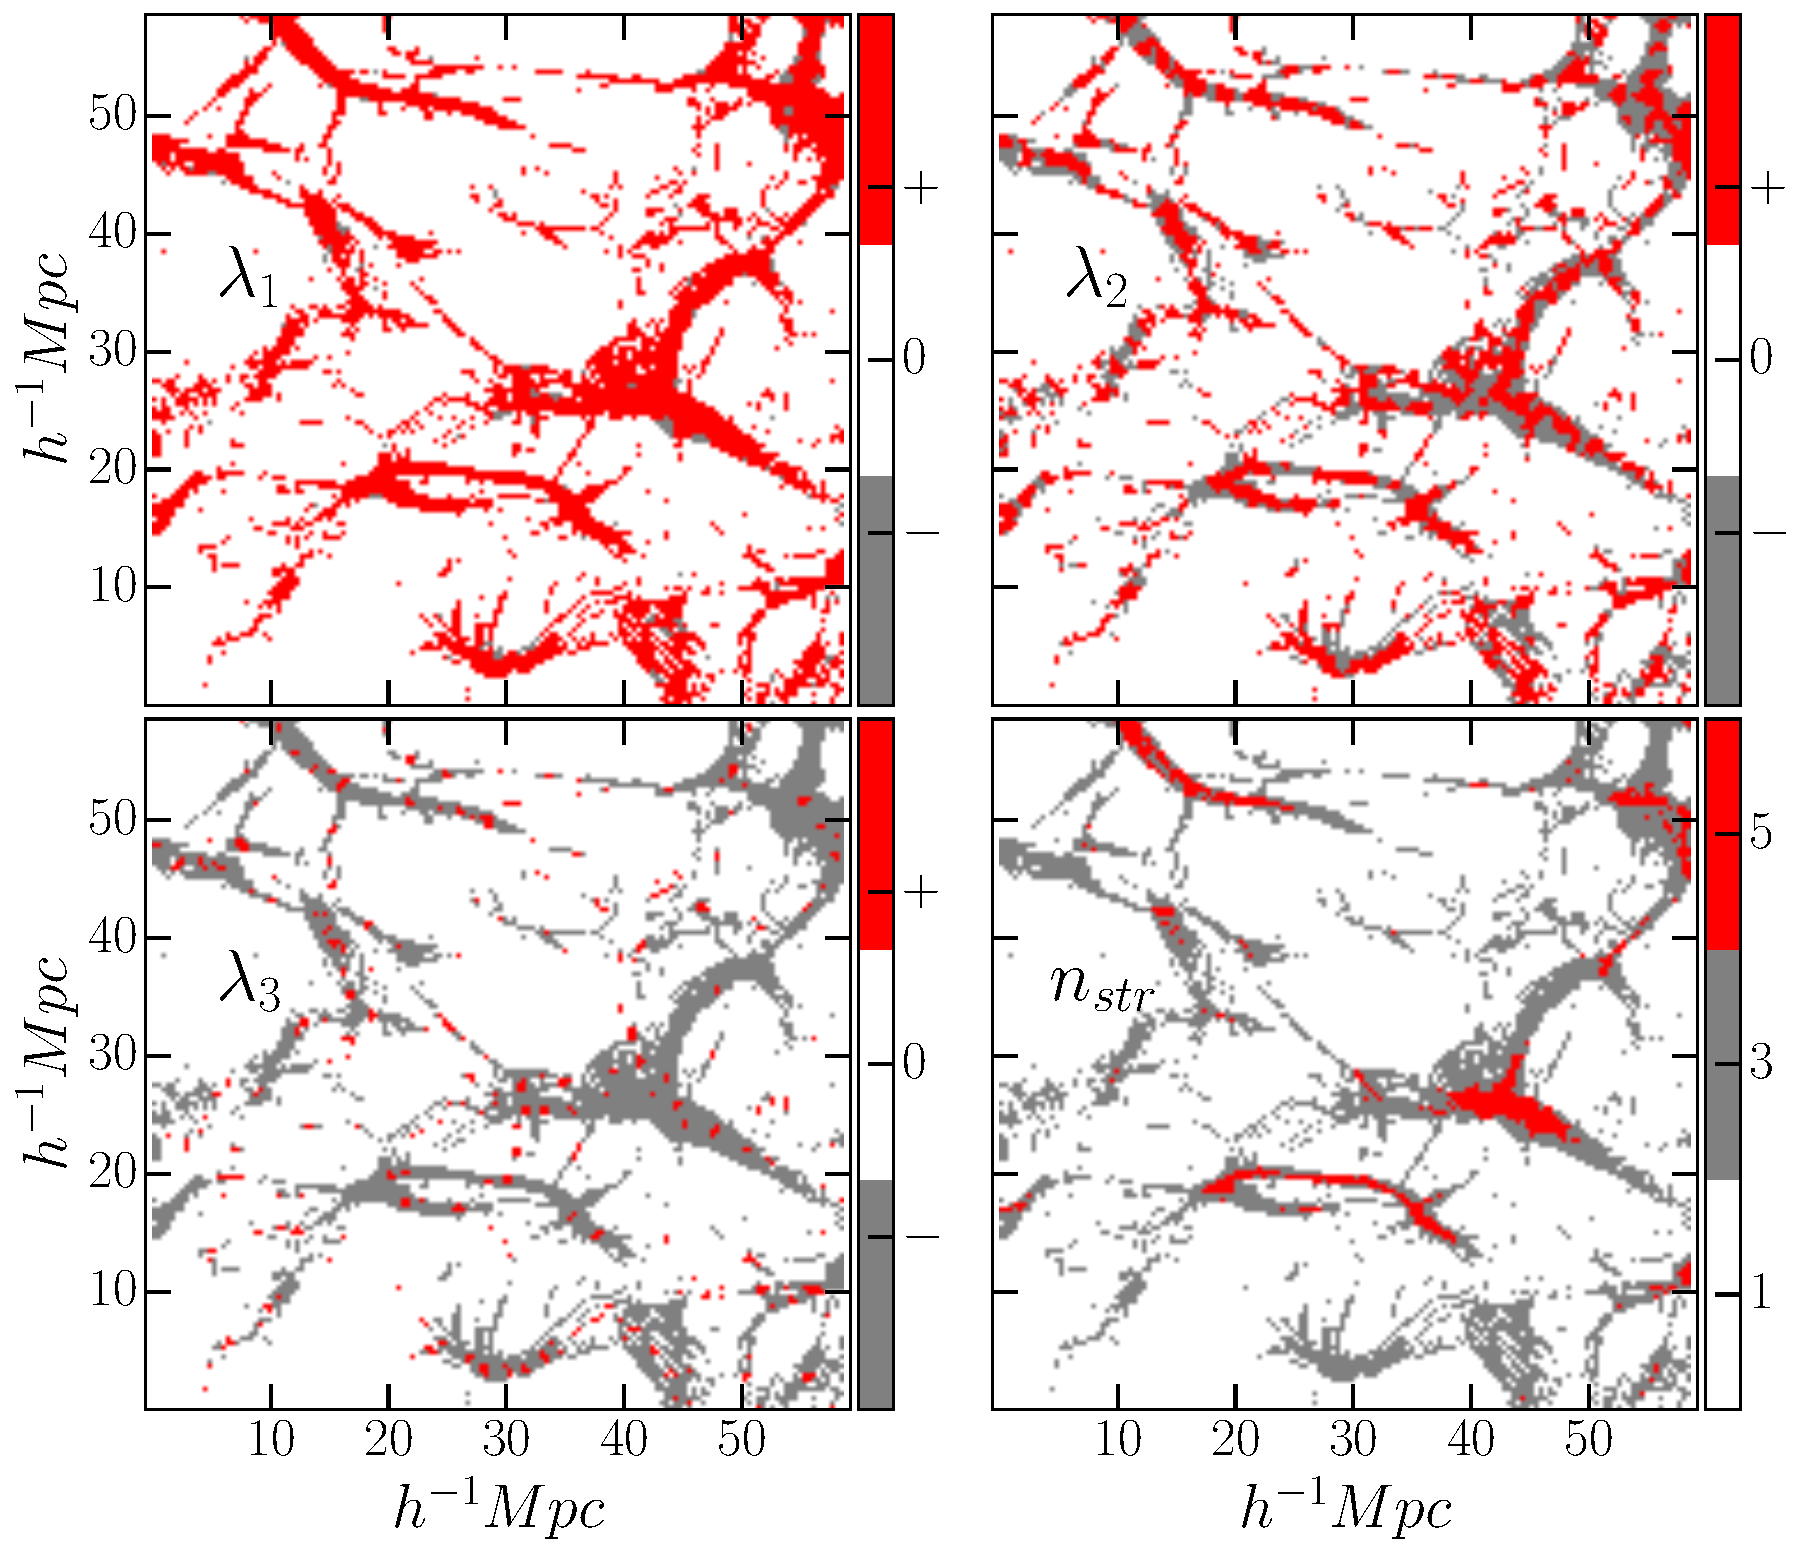
\includegraphics[height=14.cm]{Chapter4/Source_v2/fig8.pdf} 
\end{minipage}\hfill
\caption{Eigenvalues of the Hessian matrix ${\bf H}(-n_{str})$ in a slice of 50 $h^{-1}$ Mpc $\times$ 50 $h^{-1}$ Mpc slice of the simulation box of $128^3$ particles. Variation in the eigenvalues in the multistreaming web structure is shown. The largest eigenvalue $\lambda_1$ (top left panel) has positive values throughout the structure. The smallest eigenvalue $\lambda_3$ (bottom left) has negative values surrounding positive definite regions of the $n_{str}$ field. Corresponding multistream field is shown in the bottom right panel for single, three and more than five streams.}
\label{fig:evals123}
\end{figure*}

\begin{figure}
\begin{minipage}[t]{.99\linewidth}
  \centering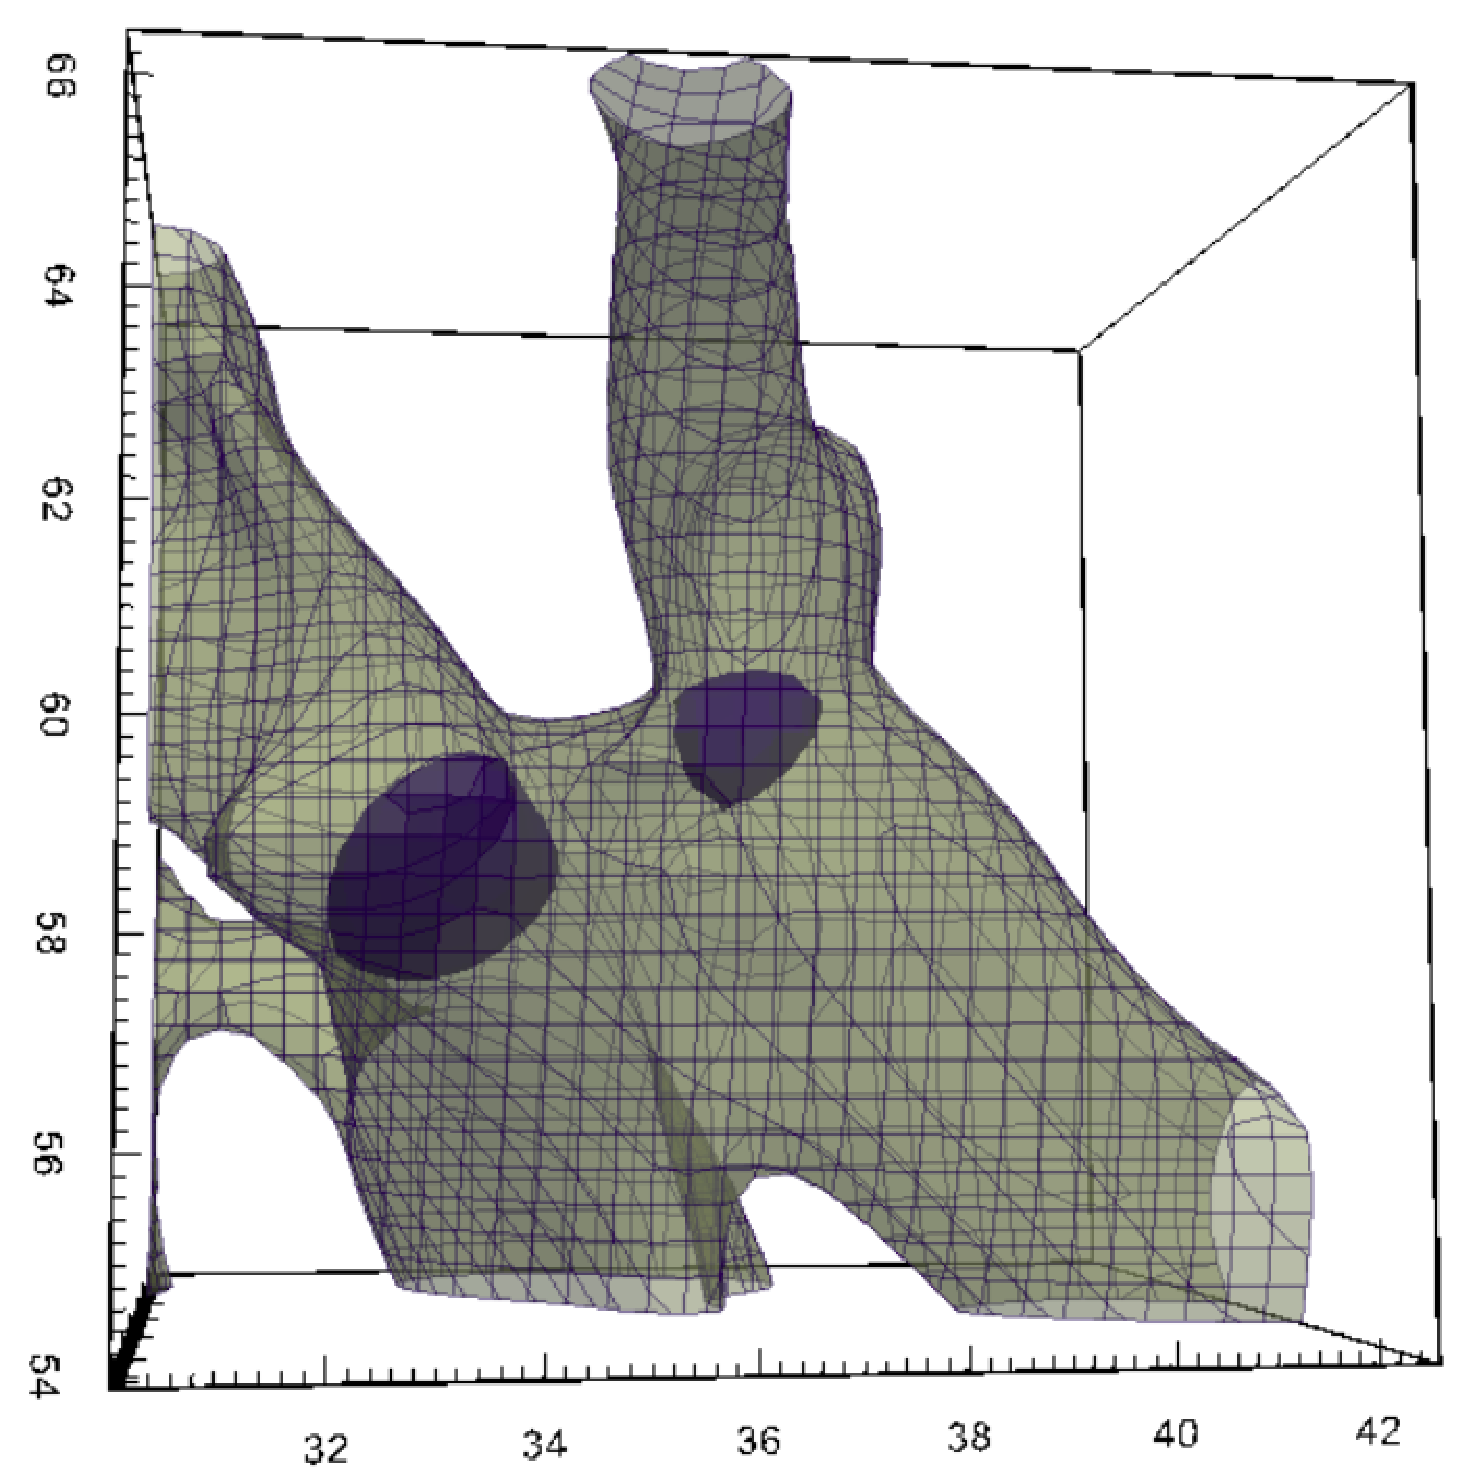
\includegraphics[width=6.cm]{Chapter4/Source_v2/fig9.pdf} 
\end{minipage}\hfill
\caption{Surfaces identified in the multistream field. Blue regions are closed regions with $\lambda_3 > 0 $, which we identify as two haloes. Other surface has an open curvature along one direction, with $\lambda_1 > \lambda_2 > 0$ and $ \lambda_3 < 0$. }
\label{fig:SmallBox}
\end{figure}

The eigenvalues of ${\bf H}(-n_{str})$ span a large range of values in our cosmological simulation. The largest eigenvalue of the triplets, $\lambda_1$ having large positive values throughout the multistream web structure ( see \autoref{fig:evals123} ). Absolute values $|\lambda_1|$, $|\lambda_2|$ and $|\lambda_3|$ peak around the neighbourhood of intersections of filaments. These junctions are usually high streaming regions due to shell crossing from multiple directions. \cite{Ramachandra2015} observed that these regions with intersecting filaments are in the vicinity of large FOF haloes. 




\begin{comment}
\begin{figure}
\begin{minipage}[t]{.99\linewidth}
  \centering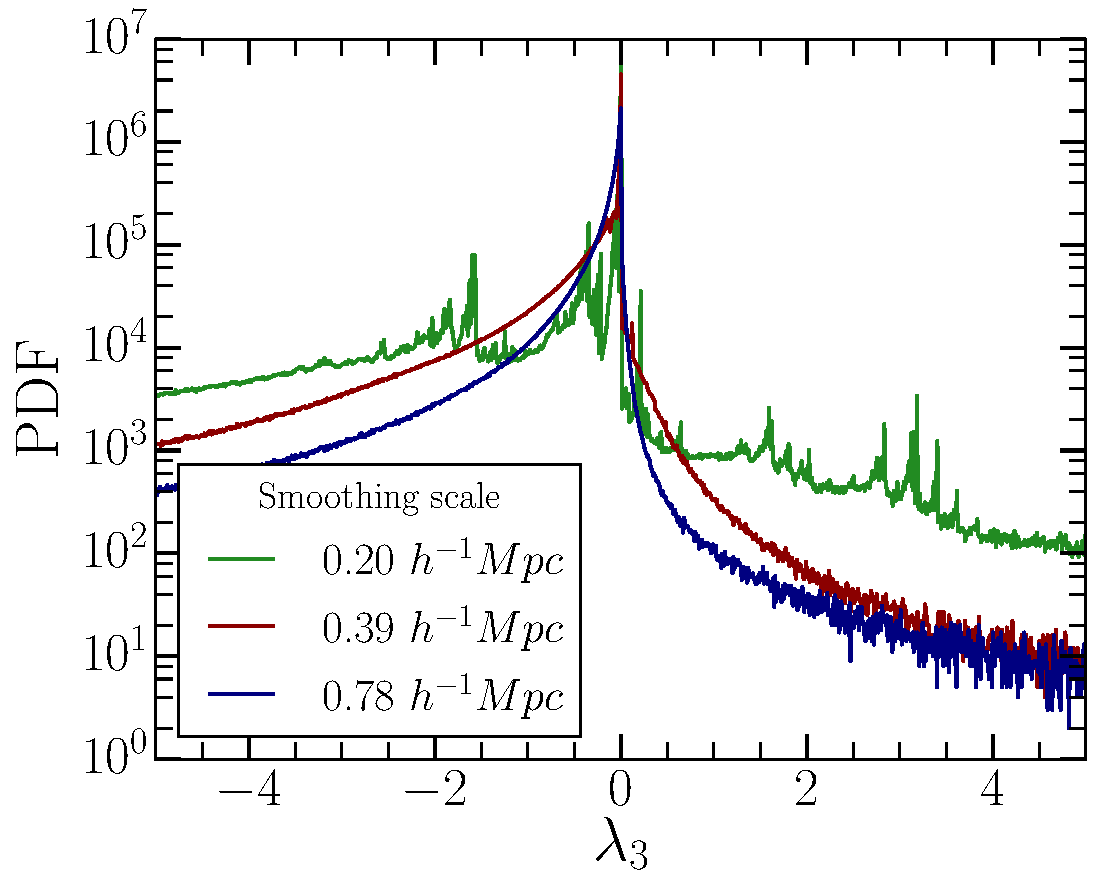
\includegraphics[width=10.cm]{fig5.pdf} 

\end{minipage}\hfill
\caption{Probability distribution function of the sorted eigenvalues of the Hessian $\mathbfss{H}(-n_{str})$ in the non-void region ($n_{str} > 1$). Total number of eigenvalue triplets are less than $10$ per cent of that of the full simulation box. Eigenvalues close to zero in non-void regions are notably fewer than in the entire simulation box.}
\label{fig:lambdasPDFNonVoid}
\end{figure}
\end{comment}


If the Hessian matrices are positive definite in a region, i.e., if all the eigenvalues are strictly positive, then the interior of this convex region has at-most one minimum. For our choice of $-n_{str}(\bf{x})$ as the domain of Hessian, this means that the convex neighbourhoods around local maxima of the multistream field are isolated by the positive definite Hessian matrices. Closed surface contours at high streaming or the most non-linear regions are selected. These regions my indeed be the regions of dark matter haloes.

The smallest eigenvalue, $\lambda_3$ has lowest volume fraction of all the eigenvalues in the positive tail of the distributions in \autoref{fig:lambdasPDF}. Since the condition $\lambda_3 > 0$ ensures the Hessian matrix to be positive definitive, we may use it as a primary criterion in isolating compact regions of dark matter haloes. These regions also roughly correspond to isolated globs as seen in \autoref{fig:SmallBox}. Local geometry analysis is pertinent for halo detection due to compact geometry of the haloes. In principle, other components of the cosmic web could also be detected. Tubular structures in filaments could be detected, as shown in \autoref{fig:SmallBox}, using conditions on the eigenvalues as $\lambda_1 > \lambda_2 > 0$ and $ \lambda_3 < 0$ . Fabric-thin walls could be detected by $\lambda_1 > 0$ and $ \lambda_3 < \lambda_2 < 0$. 
\begin{comment}
However, we only focus on using the local geometrical indicators to identify potential haloes in this study. 
\end{comment}






\subsection{Softening of the multistream field}
\label{sub:Softening}

%\hl{New sub-section, for smoothing effect of $n_{str}$ and discussion of discrete $n_{str}$ values.}

Hessian eigenvalues are generally defined on continuous functions. Although our domain of the Hessian is an inhererntly integer-valued field, it describes the multistream structure at the level of diagnostic grid. Hence it may be considered to be numerically equivalent to a continuous function where the numerical approxiamtion of differentation is a valid operation. This can be verified mathematically by finding that Hessian ${\bf H}(-n_{str})$ is symmetric (Appendix \ref{appendix:Eigen} shows the numerical approximation of the Hessian matrix term for generic unfiltered multistream field.)

Smoothing the multistream field (at the refinement level of $l_l/l_d=$ $1$ or $2$) effectively reduces noise. There is also a systematic variation in the distribution of smoothed $n_{str}$ values as shown in \autoref{fig:nstrSmooth}. Volume fraction of the single-streaming voids only varies from $90.8$ per cent without smoothing to $89.1$ per cent for the Gaussian softening length of 0.39 $h^{-1} Mpc$ (twice the length of diagnostic grid $l_d$). On the other hand, $n_{str} = 3$ regions gain volume fraction from $4.9$ per cent in un-smoothed field to $7.1$ per cent for 0.39 $h^{-1} Mpc$. This is seen in the multistream structures of smootheing scales of 0.39 $h^{-1} Mpc$ in \autoref{fig:nstrSmoothSmall}. Multi-stream regions with $ 3 < n_{str} \leq 100 $ occupy correspondingly lower volumes for higher smoothing, and the variation is noisy beyond $n_{str} > 100$. \autoref{fig:nstrSmoothSmall} shows the multistream field on a small slice of the simulation at different softening scales, and walls and filaments are resolved better with increasing softening.                                                                

%the Gaussian filters shown at softening scales equal to $0.5$, $1$, $1.5$ and $2$ times the side length of diagnostic grid $l_d$.}
%\hl{In order to reduce noise, the field is smoothed for our analysis using a Gaussian filter. The effect of smoothing scale on the distribution of the multistream values is shown in \autoref{fig:nstrSmooth}.}


\begin{comment}
The effect of smoothing scale on the distribution of the eigenvalue $\lambda_3$ in the simulation of $128^3$ particles is shown in \autoref{fig:Eval3Smooth}. 

No smooth
nstr = 1:  90.8026777208
nstr = 3:  4.86832410097
nstr > 3:  4.32899817824

0.10 $h^{-1} Mpc$
nstr = 1:  90.447498858
nstr = 3:  5.46239987016
nstr > 3:  4.09010127187

0.20 $h^{-1} Mpc$
nstr = 1:  90.0112554431
nstr = 3:  6.1724729836
nstr > 3:  3.81627157331

0.39 $h^{-1} Mpc$
nstr = 1:  89.0503048897
nstr = 3:  7.13266804814
nstr > 3:  3.81702706218

\end{comment}


Smoother multistream fields result in less noisy PDFs of the Hessian eigenvalues. For instance, the volume fraction of regions with positive curvature (i.e. $\lambda_3 > 0$) is $2.4\%$, $2.3\%$ and $2.5\%$ for scales $0.20 h^{-1} \text{ Mpc}$, $0.39 h^{-1} \text{ Mpc}$, $0.78 h^{-1} \text{ Mpc}$ respectively. Further analysis of smoothed positive definite regions is relevant in determining halo boundaries, and will be extensively discussed in the next paper. 

%at multistream smoothing scale are smoother of the half the side length of diagnostic grid , $0.5 \times l_d = 0.20 h^{-1} \text{ Mpc}$ is noisier than in the scales of $l_d$ and $2 \times l_d$. However, at every scale, the PDF peaks at $0$.  
\begin{comment}
For the detection of haloes in Section \ref{sec:haloDetection}, we only look at these regions. Multi-scale phenomena of our halo detection algorithm at different smoothing is discussed in Section \ref{sub:Smooth}. 
\end{comment}

\begin{comment}
\begin{figure}
\begin{minipage}[t]{.99\linewidth}
 \centering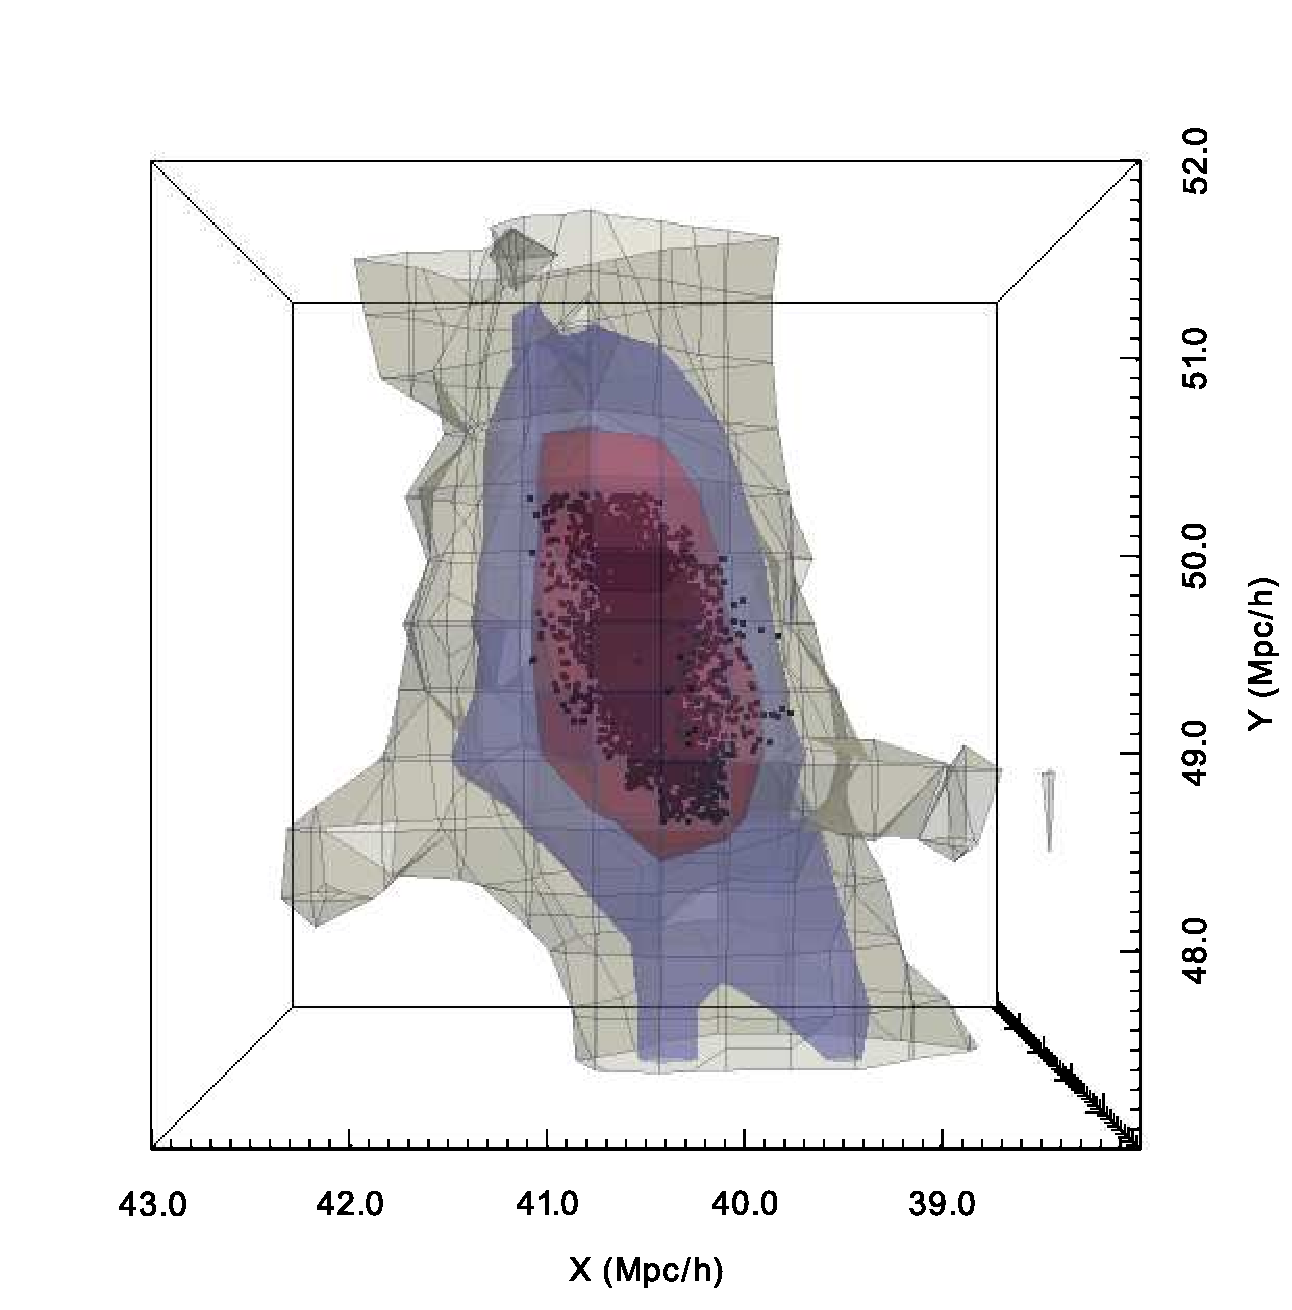
\includegraphics[width=10.cm]{fig9.pdf} 
\end{minipage}\hfill
\caption{The distribution of $\lambda_3$ in the simulation box of $128^3$ particles and multistream field of refinement factor $l_l/l_d = 2$. Three smoothing scales are shown. }
\label{fig:Eval3Smooth}
\end{figure}
\end{comment}


\begin{figure}
\begin{minipage}[t]{.99\linewidth}
  \centering\includegraphics[width=10.cm]{Chapter4/Source_v2/fig10.pdf} 

\end{minipage}\hfill
\caption{Probability distribution function of the multistream $n_{str}$ values in the simulation box with $N_p = 256^3$. The multistream field is calculated at refinement factor $l_l/l_d= 2$. Unsmoothed multistream field is compared with different Gaussian filtering scales. Softening scales of equal to $0.5$, $1$, and $2$ times the side length of diagnostic grid $l_d$ correspond to $0.10 h^{-1} \text{Mpc}$, $0.20 h^{-1} \text{Mpc}$, and $0.39 h^{-1} \text{Mpc}$ respectively.}
\label{fig:nstrSmooth}
\end{figure}

\begin{figure}
\begin{minipage}[t]{.99\linewidth}
  \centering\includegraphics[width=10.cm]{Chapter4/Source_v2/fig11.pdf} 

\end{minipage}\hfill
\caption{Multi-stream field at various softening scales in the simulation box with $N_p = 256^3$. The multistream field is calculated at refinement factor $l_l/l_d= 2$. Unsmoothed multistream field is compared with different Gaussian filtering scales equal to $0.10 h^{-1} \text{Mpc}$, $0.20 h^{-1} \text{Mpc}$, and $0.39 h^{-1} \text{Mpc}$ respectively.}
\label{fig:nstrSmoothSmall}
\end{figure}

%Analysis of a non-zero eigenvalue thresholds on the same Hessian is done by \cite{Forero-Romero2009a}, where they argued that volume fraction of the void is higher for positive values of the thresholds. They also concluded that smoothing scales do not play an important role in the volume fractions of the classified structures. 


\subsection{Resolution dependence}
\label{sub:resolution}

Multi-stream calculation can be done at arbitrarily high resolutions by populating the tetrahedral simplices. For our resolution study, we have chosen a smaller slice of $ 50 h^{-1} \text{Mpc} \times 50 h^{-1} \text{Mpc} \times 50 h^{-1} \text{Mpc}$ (grid of size $64^3$ from the N-body simulation) from the simulation with $N_p = 128^3$ particles. The multistream field is calculated at 4 different refinement factors, i.e., at diagnosis grids of size $64^3$ ($l_l/l_d = 1$), $128^3$ ($l_l/l_d = 2$), $256^3$ ($l_l/l_d = 4$)  and $512^3$ ($l_l/l_d = 8$) respectively.

Volume fractions of each multistream does not change systematically for different levels of refinement, except at very high $n_{str}$ values (see \citealt{Ramachandra2015} for dependence of $n_{str}$ variation on refinement of the diagnostic grid). At high multistream values, higher resolutions reveal a considerably less noisy multistream fields. 

There are no variations in the volume fractions of the cosmic web components classified using the global $n_{str}$ thresholds as shown in \autoref{tab:VolfrRefNst}. Voids ($n_{str} = 1$) occupy about 90 per cent of the volume at each refinement factor. Rest of the heuristic thresholds that identify the structure components (as prescribed by \citealt{Ramachandra2015}) are constant multistream contours: $3 \leq n_{str} < 17$ for walls, $17 \leq n_{str} < 90 $ for filaments and $n_{str} \geq 90 $ for haloes. Since the volume fraction of each $n_{str}$ values are about the same at each refinement factor, the volume fraction of the cosmic web components corresponding to global multistream thresholds do not vary considerably. 


\begin{table}
\centering
\caption{Volume fraction (in per cent) of $n_{str}$ thresholds for cosmic web structures as defined by \protect\cite{Ramachandra2015}. Multi-stream field is calculated at 1, 2, 4, and 8 times the native simulation resolution of $64^3$ grids. Small slice of $ 50 h^{-1} \text{Mpc} \times 50 h^{-1} \text{Mpc} \times 50 h^{-1} \text{Mpc} $ is chosen for the analysis.}
\begin{tabular}{|l|l|l|l|l|}
\hline
Global thresholds  & $64^3$   & $128^3$   & $256^3$  & $512^3$ \\  \hline
$n_{str} = 1$ (Void)     &    90.87   & 90.92  & 90.94 & 90.94 \\ \hline
$3 \leq n_{str} < 17$ (Wall)  & 8.71 & 8.66 & 8.63 & 8.64   \\ \hline
$17 \leq n_{str} < 90 $ (Filaments) &  0.39 & 0.39 & 0.39 & 0.39    \\ \hline
$n_{str} \geq 90 $ (Haloes) & 0.034 & 0.035 & 0.036 & 0.036 \\ \hline

\end{tabular}
\label{tab:VolfrRefNst}
\end{table}



However, local geometry analysis of the multistream flow field varies considerably on the resolution of the analysis grid. For our Hessian ${\bf H}(-n_{str})$, the regions with $\lambda_1 \geq \lambda_2 \geq \lambda_3 > 0$ in non-void regions occupy 1.8 per cent of the entire box in native resolution of diagnostic grid, as shown in \autoref{tab:VolfrRefLambda}. This fraction reduces to 1.3 per cent at diagnostic grid of $512^3$ resolution. Variations with refinement factors are seen in other eigenvalue conditions in the non-void too: volume fraction of $\lambda_1 > 0 > \lambda_2 \geq \lambda_3 $ regions increases from 1.7 per cent at refinement factor of 1 to 3 per cent at refinement factor of 8. Volume fraction of $\lambda_1 \geq \lambda_2 > 0 > \lambda_3 $ regions decreases from 5.6 to 4.6 per cent with the increase of refinement from 1 to 8. 

In principle, the conditions for geometric criteria are: $\lambda_1 > 0 > \lambda_2 \geq \lambda_3$ for locally flat regions, $\lambda_1 \geq \lambda_2 > 0 > \lambda_3 $ for locally tubular structures and $\lambda_1 \geq \lambda_2 \geq \lambda_3 > 0$ for clumped blobs. However, the tabulated the volume fractions in \autoref{tab:VolfrRefLambda} does not correspond to cosmic web components themselves. Identification of the components may require post processing steps. 
\begin{comment}For detection of dark matter haloes, the algorithm prescribed in Section \ref{sec:haloDetection} lists out a set of physically motivated processes that filter out the noisy $\lambda_1 \geq \lambda_2 \geq \lambda_3 > 0$ regions that cannot be identified as haloes.
\end{comment}

High resolution studies of multistream fields would play an important role in detection of walls and filaments. These two components have smaller length scales along at least one direction with respect to others. As seen in Section \ref{sec:voidPerc}, walls are more resolved in high resolution of multistream fields, enclosing pockets of voids (see \autoref{fig:voidFace}).  

However, a Hessian analysis to identify filaments and walls may be considerably different from that of halo finding due to the following reasons: First, a local geometrical analysis is uniquely convenient for detecting dark matter haloes since they are local structures. Filaments and walls, alternatively, are structures that span over large distances. Secondly, we try to find regions around local maxima of multistream field for haloes. Whereas, filaments and walls have much weaker relationship with local multistream maxima. Filaments and walls usually deviate from flat planar or straight tubular geometries: they often have complicated structures several connections and branches. For these reasons, Hessian eigenvalues alone would not be sufficient in detecting walls or filaments. 
\begin{comment}
In our analysis in Section \ref{sec:haloDetection}, we only concentrate on halo detection using local geometry indicators. Hessian analysis for identifying walls and filaments are beyond the scope of this paper. 
\end{comment}



\begin{table}
\centering
  \caption{Volume fraction of criteria based on $n_{str}$ and $\lambda$s of ${\bf H}(-n_{str})$ calculated at various resolutions. We chose a smaller slice of $ 50 h^{-1} \text{Mpc} \times 50 h^{-1} \text{Mpc} \times 50 h^{-1} \text{Mpc} $ i.e., half the volume of the original GADGET simulation box. The refinement factors are the multiplication factors of 1, 2, 4 and 8 times of the native resolution ($64^3$) of the simulation grid along each axis. Eigenvalues of the Hessian of the field are local geometric parameters. The void is globally defined as $n_{str} = 1$ and the multistream web structure as $n_{str} > 1$.}


\begin{tabular}{|l|l|l|l|l|}
\hline
Global/local conditions & $64^3$   & $128^3$   & $256^3$  & $512^3$  \\  \hline
$n_{str} = 1$ (Void)     &    90.87   & 90.92  & 90.94 & 90.94 \\ \hline
$n_{str} > 1$; $\lambda_1 > 0 > \lambda_2 \geq \lambda_3 $  &  1.72 & 2.22 & 2.67 & 2.96    \\ \hline
$n_{str} > 1$; $\lambda_1 \geq \lambda_2 > 0 > \lambda_3 $ & 5.60 & 5.28 & 4.91 & 4.57   \\ \hline
$n_{str} > 1$; $\lambda_1 \geq \lambda_2 \geq \lambda_3 > 0$ & 1.81 & 1.56 & 1.37 & 1.26 \\ \hline

\end{tabular}
\label{tab:VolfrRefLambda}
\end{table}

\begin{comment}

\section{Haloes in the multistream field}
\label{sec:haloDetection}

    
We intend to identify haloes in the $n_{str}(\bf{x})$ field instead of using just the position coordinate data. While the eigenvalue analysis itself is done at a chosen time, the multistream field inherently has data from six-dimensional Lagrangian space $(\bf{q}, \bf{x})$ that contains the full dynamical information,similar to the phase-space sheet albeit in a different form. Dynamical history that is embedded in the multistream field is crucial in understanding the strength of gravitational binding of the particles. 
Moreover, as explained in Section \ref{sec:voids}, a physically motivated distinction between void and gravitationally collapsed regions is a unique feature of multistream analysis. Thus the haloes detected from local maxima of the $n_{str}$ field can be ensured to be away from the single streaming voids. Methods based on linking-length or density fields may not able to ensure that all the particles in haloes are away from voids, as shown for FOF method in Section \ref{sec:voidHaloes}. 


Numerical analyses of scalar fields generally depend on resolution as opposed to particle coordinates analysis tools like FOF. The multistream field conveniently has an advantage of being less noisy than mass density (\citealt{Shandarin2012}, also see Appendix \ref{appendix:nstream}). For the illustration halo detection framework in this section, we have calculated the number-of-streams at refinement factor of 2 and smoothing scale of $0.39 h^{-1} Mpc$ (equal to the grid length of the multistream field) for the simulation box of $128^3$ particles and size $L = 100 h^{-1} Mpc$. Hessian matrices and eigenvalues are calculated on the same diagnosis grid. Results of the halo detection scheme for simulation box of higher mass resolution, and different smoothing factors are discussed in Sections \ref{sub:compareHalo} and \ref{sub:Smooth}. Hereafter we refer to the potential dark matter haloes detected from the Hessian analysis of the multistream field as $\lambda_3$-haloes for brevity. Similarly, the haloes candidates from AHF and FOF algorithms are referred to as AHF-haloes and FOF-haloes respectively. 


\subsection{Halo finder algorithm}
\label{subsec:technique}



Our goal is to isolate the locations of convex geometries in the multistream flow field. Prospective regions of the halo locations in the web structure are selected by positive definite condition of the Hessian $\mathbfss{H}(-n_{str})$: $\lambda_1 > 0$, $\lambda_2 > 0$ and  $\lambda_3 > 0$, or simply the smallest of the eigenvalues, $\lambda_3 > 0$. We also filter out the regions if the multistream values inside do not suggest gravitational collapse into haloes. The sequence of our halo detection framework is listed below: 


\begin{enumerate}
\item The multistream flow field is calculated on a diagnostic grid. The number of tetrahedra that encompass each vertex in the grid gives the $n_{str}$ field. Top left panel of \autoref{fig:labelsfilter} shows the multistream web structure in a slice of the simulation with $n_{str} > 1$ in gray and $n_{str} \geq 7$ in blue.  

\item The discrete multistream flow field is smoothed in order to reduce numerical noise. We have used Gaussian kernel for smoothing in our analysis. Effect of smoothing scales in the halo identification is discussed in Section \ref{sub:Smooth}. 

\item Second order variations of the smoothed $-n_{str}(\bf{x})$ is computed at each point in the field. This gives symmetric Hessian matrices for this field whose eigenvalues are real. Ordered eigenvalues of the Hessian, $ \lambda_1 \geq  \lambda_2 \geq \lambda_3$ are calculated. The $\lambda_3$ field is shown in the top right panel of \autoref{fig:labelsfilter}. 

\item Using segmentation techniques, each region with $ \lambda_3 $ strictly greater than $0$ within $n_{str} \geq 3$ regions of multistream field are isolated and labelled. This condition for each halo candidate guarantees that it is in the region where at least one gravitational collapse happened within the halo boundary. Mass particles belonging to these regions are shown shown as dark spots in in the top right panel of \autoref{fig:labelsfilter}. 

\item The multistream field has a range of values within the isolated sites. We impose constraints on the isolated regions to rule out the labels with low multistream values. The local maxima of $n_{str}$ inside each halo must be at least 7. By this restriction, it is ensured that the halo sites with three Lagrangian sub-manifold foldings are selected. Bottom left panel of \autoref{fig:labelsfilter} shows patches that are discarded in red. The resulting $\lambda_3$-haloes are shown in the bottom right.  
  

\item In our comparisons with other halo finders in Section \ref{sub:compareHalo}, we also used an additional constraint on the minimum number of mass particles in the haloes to be 20 - which is generally used as a criteria in several halo finders. 

\end{enumerate} 


\begin{figure}
\begin{minipage}[t]{0.99\linewidth}
 \centering\includegraphics[height=8.5cm]{fig10.pdf} 
\end{minipage}\hfill
\caption{ Detection of potential halo candidates in the multistream field: algorithm of segmentation and filtering are illustrated in a smaller slice of $40 h^{-1} Mpc \times 40 h^{-1} Mpc$ slice of the simulation box. Top left figure shows the multistream field of the slice. Voids (white) are the regions with $n_{str} =1$, rest are non-void structures. Blue patches within the structure (gray) are the regions with gravitational collapses in more than one direction, i.e., $n_{str} \geq 7$. Top Right figure shows the smallest eigenvalue $\lambda_3$ field. The value of $\lambda_3$ is close to 0 in most of the regions (yellow), including the voids. Regions with  $\lambda_3 > 0$ and $n_{str} > 1$, are isolated (black spots) using image segmentation techniques. Bottom left panel shows the filtering scheme: the red patches do not have maxima of $n_{str} \geq 7$ in the regions, hence are filtered out. The remaining potential halo regions with more than 20 particles are shown in the bottom right panel.}
\label{fig:labelsfilter}
\end{figure}

 

Applying the above scheme on the simulation with side length of $100 h^{-1}$ Mpc and $128^3$ particles (with cosmological parameters mentioned in Section \ref{sec:simulation}), we detected approximately 50000 regions satisfying $\lambda_3 > 0$ within the non-void in the multistream field of refinement factor $l_l/l_d = 2$ and smoothing scale of grid length, i.e, $0.39 h^{-1} Mpc$. We filtered out the segments with local maxima of $n_{str} < 7$, and around 14000 regions remained as prospective haloes. On the whole, our algorithm detected about 4500 haloes with more than 20 particles in the entire simulation box. The halo candidates we obtained are generally observed to be compact. We have not applied virialisation to define the halo boundaries. A more detailed study of halo edges, and comparison with that of FOF-haloes and AHF-haloes is done in Section \ref{sub:HaloProperties}.

The maximum values of $\lambda_1$, $\lambda_2$ and $\lambda_3$ in each of the haloes have peaks away from 0 as shown in \autoref{fig:maxL3}. The median values of $max(\lambda_1)$ and $max(\lambda_2)$ are in the range of 1-10 (\autoref{tab:maxL3}), in-spite of the threshold for $\lambda_3$ being barely positive, by definition. Hence the interior of the potential halo segments is quite convex, with a local maxima inside. In some haloes, the local maxima of eigenvalue are in the order of thousands, as tabulated in \autoref{tab:maxL3}. 


\begin{figure}
\begin{minipage}[t]{.99\linewidth}
 \centering\includegraphics[width=10.cm]{fig11.pdf} 
\end{minipage}\hfill
\caption{PDF of highest $\lambda_1$, $\lambda_2$ and $\lambda_3$ values in each of 4492 haloes detected by out algorithm. The peaks of the PDF are in the range 1-10. Shaded regions represent 1$\sigma$ error. }
\label{fig:maxL3}
\end{figure}

\begin{table}
  \caption{Statistics of the the Hessian eigenvalues in halo candidates: Local maxima of $\lambda_1$, $\lambda_2$ and $\lambda_3$ in each of 4492 haloes are shown. }
\begin{tabular}{|l|r|r|r|}
\hline
Statistics                &  $\lambda_1$ &  $\lambda_2$ &  $\lambda_3$\\ \hline
Minimum   & $ 1.5 $ & $ 0.5 $ & $ 1.3 \times 10^{-2} $  \\ \hline
Maximum  & $1.7 \times 10^3$  & $1.5 \times 10^3$ & $1.1 \times 10^3$     \\ \hline
Median     & $10.5$  & $5.5$ & $1.9$  \\ \hline
\end{tabular}
\label{tab:maxL3}
\end{table}

 
With this algorithm, we obtain prospective dark matter haloes - regions with a local maximum of the multistream field in the interior of their closed surfaces. The haloes are detected without using density fields or linking lengths between particles. The parameters in the algorithm are entirely based on features of the multistream field and local geometry using Hessian matrices. 


\subsection{Halo properties}
\label{sub:HaloProperties}

Multi-stream environment of haloes can be very diverse. \cite{Ramachandra2015} demonstrated that a majority of the FOF-haloes are in contact with the single-streaming voids. Illustration in \autoref{fig:Vfr_all} also shows that a large number of FOF-haloes have more than 10 per cent void on the spherical surfaces with virial radii. The $\lambda_3$ haloes are significantly different: none of the $\lambda_3$-haloes are in contact with the regions where gravitational collapse has not occurred. This is guaranteed by the lower bound of $n_{str} = 3$ on all potential halo candidates. 

Condition on the multistream field within the $\lambda_3$-halo also ensures that there are collapses along more than one direction, which corresponds to $n_{str} = 7$. For a large number of $\lambda_3$-haloes candidates, the maximum $n_{str}$ is higher than this threshold, as shown in \autoref{tab:minmaxstr} and \autoref{fig:minmaxstr}. The regions selected by $\lambda_3 > 0$ on Hessian of $-n_{str}$ have a maxima of $n_{str}$ within their boundaries. For simulation with $128^3$ particles, the median of this peak $n_{str}$ value is $17$. Unsurprisingly, the global maximum of the multistream field ($n_{str} = 2831$) is also a local maximum for one of the haloes. On the other hand, the median of minimum $n_{str}$ in the haloes is 3 (\autoref{tab:minmaxstr}), which is also the first stage of non-linearity.


\begin{figure}
\begin{minipage}[t]{.99\linewidth}
 \centering\includegraphics[width=10.cm]{fig12.pdf} 
\end{minipage}\hfill
\caption{Maximum, minimum and median of $n_{str}$ in each of 4492 halo candidates. The closed contours of haloes encompass a wide range of multistream values. None of the haloes are in contact with the void region, since lowest value of min$(n_{str})$ is 3. Shaded regions are the 1$\sigma$ absolute errors in the number of $\lambda_3$-haloes. }
\label{fig:minmaxstr}
\end{figure}


\begin{table}
\caption{Local maxima and minima of $n_{str}$ in each of 4492 haloes. The highest $n_{str}$ values in the interior of haloes span over a large range of values. Low values of $n_{str}$ in haloes, which are generally near halo boundaries, have a median of 3.}
\begin{tabular}{|l|r|r|}
\hline
Statistics  &  high $n_{str}$ & low $n_{str}$ \\ \hline
Minimum     & $7$    & $3$  \\ \hline
Maximum     & $2831$ & $459$      \\ \hline
Median      & $17$   & $3$   \\ \hline
\end{tabular}
\label{tab:minmaxstr}
\end{table}


An important feature of our halo detection method is that the detected $\lambda_3$-haloes do not have a global threshold on $n_{str}$ or mass density values. The local conditions may be more suited in identifying haloes in multistream fields, since the multistream environments around haloes are very diverse. For instance, regions with $n_{str} \geq 25$ is tubular around one of the the large haloes in \autoref{fig:l3Nst}. Even the region with more than $75$ streams does not enclose a convex multistream region. Whereas, for $n_{str} \geq 200$ the region is convex and the particles detected by our method reside mostly within. We detect closed regions in the multistream field as long as they are not in void, and have gravitational collapse in more than one directions.  

However, the $\lambda_3$-halo boundary is different from any constant multistream contour. That is, from the function $n_{str}(\bf{x})$, convex regions in the four-dimensional function space $(-n_{str}, x, y, z)$ are projected onto three-dimensional co-ordinate space using eigenvalues. This is different from projecting `iso-multistream' slice onto three-dimensional co-ordinate space. Appendix \ref{appendix:Eigen} illustrates the difference in the two approaches for a one-dimensional function. 


The multistream field usually has concentric shells in the regions of successive gravitational collapses (as explained in Section \ref{sec:multiCalc} and Appendix \ref{appendix:nstream}). In a specific scenario of \autoref{fig:l3Nst}, regions of lower number-of-streams ($n_{str} = 25$ and lower) is tubular and has regions of higher $n_{str}$ inside ($n_{str} = 200$ and higher) that is closed. However, this transition from concavity to convexity of the multistream field does not occur at a constant value of $n_{str}$ throughout the field. Instead, it is a local geometrical change that occurs at $\lambda_3 = 0$. For the $\lambda_3$-haloes in this simulation, a range of minimum $n_{str}$ for each halo has a range of values, as shown in \autoref{tab:minmaxstr} and \autoref{fig:minmaxstr}. Hence a global condition on $n_{str}$ does not guarantee that the region is closed. 



\begin{figure}
\begin{minipage}[t]{.99\linewidth}
  \centering\includegraphics[width=7.cm]{fig13.pdf} 
\end{minipage}\hfill
\caption{Multi-stream environment of a $\lambda_3$-halo. The contours represent regions with 3 different multistream values: Outermost $n_{str} \geq 25$ (gray) is tubular, The blue region has $n_{str} \geq 75$. The inner region is highly non-linear with $n_{str} \geq 200$.  The black dots represent the mass particles belonging to a $\lambda_3$-halo, as detected by our algorithm.}
\label{fig:l3Nst}
\end{figure}



The particles in a massive $\lambda_3$-halo shown in \autoref{fig:l3Nst} form a spheroidal structure. The number of particles in similar massive haloes are in the order of $10^3$ particles. For instance, the most massive halo in the simulation (with $N_p = 128^3$) has $5593$ particles. We have chosen a minimum threshold of 20 particles, which is an artificial parameter used by most halo finder methods. Majority of the $\lambda_3$-haloes have low number of particles; median of number of particles per halo is $49$. Each particle in this simulation is approximately $ 3.65 \times 10^{10} h^{-1} M_{\sun}$. Hence the halo mass range varies in the order of $10^{11} M_{\sun}$ to $10^{14} M_{\sun}$. Combined mass of all the $\lambda_3$-halo candidates is about $31$ per cent of the total mass in the simulation. In contrast, the haloes occupy just $0.3$ per cent of the total volume. Thus the $\lambda_3$-haloes are extremely dense structures. Further analysis of halo mass function of $\lambda_3$-haloes and comparison with AHF- and FOF-haloes is done in the Section \ref{sub:compareHalo}.  


\subsection{Correspondence with other halo finders}
\label{sub:compareHalo}


Comparison of haloes obtained from AHF and FOF method, along with our geometric analysis of the multistream field reveals several interesting features. The number of haloes with at least 20 particles that were detected by all the algorithms is shown in \autoref{tab:HaloFinderMF}. For both the simulations, FOF detects the highest number of haloes and AHF detects the least. By applying the Hessian algorithm on multistream fields smoothed at the scale of diagnostic grid size, $l_d$, we detected around $4500$ and $28000$ haloes in simulations with $128^3$ and $256^3$ particles respectively. Multi-stream field both the simulations has a refinement factor of $l_l/l_d = 2$. 

\begin{table}
  \caption{Number of haloes detected by the three halo finder algorithms in the two simulations of $L = 100 h^{-1} \text{Mpc}$ with different mass resolutions. Values shown for $\lambda_3$-haloes are done in the multistream fields with refinement factor of 2, and smoothing scale equal to the diagnostic grid size.}
\begin{tabular}{|l|r|r|r|}
\hline
$N_p$  &  AHF & FOF & $\lambda_3$ \\ \hline
$128^3$   & 3374  &  5440 & 4492 \\ \hline
$256^3$   & 24710  & 35765 & 27929 \\ \hline

\end{tabular}
\label{tab:HaloFinderMF}
\end{table}

Mass fraction of the halo particles in the simulation are shown in a Venn diagram in \autoref{fig:HaloFinderMF}. For the simulation with $128^3$ particles, AHF-, FOF- and $\lambda_3-$haloes occupy $22$, $35$ and $31$ per cent of the total mass respectively. For simulation with $256^3$ particles, the corresponding halo mass fractions are $30$, $42$, and $32$ per cent respectively. However, large fractions of these mass particles are concurrently detected as belonging to haloes by different methods. As shown in \autoref{fig:HaloFinderMF}, $19-23$ per cent of the mass particles are detected by all three halo finder methods as belonging to halo regions. 


\begin{figure}
\begin{minipage}[t]{.99\linewidth}
 \centering
 \includegraphics[width=10.cm]{fig14}
\end{minipage}\hfill
\caption{Mass fractions (in per cent) of haloes detected by the three finders. The particles concurrently detected as belonging to haloes are shown in the intersections. }
\label{fig:HaloFinderMF}
\end{figure}



The halo mass functions from all three finders are shown in \autoref{fig:hmf}. For smaller haloes of order of $10^{13} M_{\sun}$, our method predicts a slightly higher number of haloes than FOF and AHF. For the most massive haloes of mass around $10^{14} M_{\sun}$, number of $\lambda_3$-haloes is fewer than the other 2 methods, albeit around the range of error. 


\begin{figure}
\begin{minipage}[t]{.99\linewidth}
 \centering\includegraphics[width=10.cm]{fig15.pdf} 
\end{minipage}\hfill
\caption{Halo Mass functions from AHF-, FOF- and $\lambda_3$-haloes. The AHF-haloes are fewer than FOF- or $\lambda_3$-haloes. The number of haloes above a mass threshold are binned and taken along vertical axis, normalized to simulation box volume. Error of 1$\sigma$ is shown in shaded region. }
\label{fig:hmf}
\end{figure}


By observing some of the massive haloes, like the one in \autoref{fig:FinderCompareAll}, we find that the $\lambda_3$-halo particles are within AHF- or FOF-halo region. This is generally observed in other massive haloes too: the large $\lambda_3$-haloes have fewer particles than corresponding AHF- or FOF-haloes. For haloes greater than $10^{14} M_{\sun}$, $\lambda_3$-haloes have boundaries slightly within the AHF virial radius. Without unbinding, the FOF-haloes can be very large compared to other methods, as seen in \autoref{fig:FinderCompareAll}. This results in a deviation in the $\lambda_3$-halo mass function (\autoref{fig:hmf}) from the other two methods over halo mass of $10^{14} M_{\sun}$. Further discussion of size of the detected $\lambda_3$-haloes in the context of smoothing of the multistream is done in Section \ref{sub:Smooth}.   


\begin{figure}
\begin{minipage}[t]{.99\linewidth}
 \centering
 \includegraphics[width=10.cm]{fig16.pdf}
\end{minipage}\hfill
\caption{A large halo that was detected by AHF (red), FOF (blue) and our geometric analysis in the multistream field (green). Halo boundary differs for each halo finder method. AHF detects particles within a sphere of virial radius. FOF-halo is irregularly shaped. $\lambda_3$-halo particles are in a non-spherical, yet compact structure. }
\label{fig:FinderCompareAll}
\end{figure}



The particles identified by the AHF as belonging to haloes form spherical structures due to a series of processes (including virialization) applied to unbind the particles. Inherently, the iso-density contours at virial levels are not spherical or spheroidal. The virialized AHF-haloes on the web are shown in the left panel of \autoref{fig:FinderCompare3}. However, the spherical AHF-haloes are fewer in number compared to the other methods. 

The popular choice of linking length of $b=0.2$, although corresponding to virial density, does not ensure that the haloes have positive curvature. Most algorithms based on the FOF method re-define the halo boundaries by unbinding the particles outside a truncation radius. This truncation radius maybe the distance from the centre of mass of the halo to the farthest particle, rms distance, or an inflection point in the density field (For details on these methods, see \citealt{Knebe2011a} and references therein). Some halo finders define the virial radius, $r_{vir}$ at the distance from halo center where the density is $\Delta_{vir}$ times the background density. In the middle panel of \autoref{fig:FinderCompare3}, the FOF-haloes are shown without any of the above post-processing schemes. Without any unbinding, the FOF-haloes are generally larger in size than $\lambda_3$-haloes in the right panel of \autoref{fig:FinderCompare3}. For a specific case of a massive halo, \autoref{fig:FinderCompareAll}, FOF identifies more particles as bounded, than AHF or our algorithm.  

 
\begin{figure*}
\centering

\includegraphics[width=5.8cm]{fig17a.pdf}  
\includegraphics[width=5.8cm]{fig17b.pdf} 
\includegraphics[width=5.8cm]{fig17c.pdf}  

\caption{Potential haloes detected by AHF (left), FOF (centre) and our analysis (right). Most of the haloes are embedded in a percolating filament with $n_{str} \geq 9$. AHF-haloes are spherical by definition. FOF-haloes without any post processing are elongated along the filament. $\lambda_3$-halo candidates are neither spherical, nor elongated. Boundaries of $\lambda_3$-haloes are well resolved. } 
\label{fig:FinderCompare3}
\end{figure*}



In contrast to the AHF and FOF algorithms, our halo method directly detects a closed compact surface (approximately the largest one, since $\lambda_3 >0$) for each of the haloes. There is no unbinding procedure on the particles identified within the halo site. The $\lambda_3$-haloes themselves are not spherical or of any regular structure, but they are closed, as seen in the right panel of \autoref{fig:FinderCompare3}. 


Haloes from the three finders in \autoref{fig:FinderCompare3} also show other differences in the halo boundaries. While all the AHF-haloes are spherical, the FOF-haloes are irregular. The $\lambda_3$ haloes are not spherical either, but are more compact than FOF-haloes. At some junctions of the filaments, FOF identifies a large region as belonging to single halo, whereas AHF and our algorithm detect multiple isolated haloes. Each isolated $\lambda_3$-halo region enclose one maximum of multistream field, thus guaranteeing that multiple haloes are always resolved. On the other hand, a linking length cut-off or a constant threshold on scalar fields may enclose regions with multiple local maxima ( For one-dimensional fields, an illustration of this is shown in Appendix \ref{appendix:Eigen}). 
 


\subsection{Effect of smoothing}
\label{sub:Smooth}

In addition to reducing the numerical noise (Section \ref{sec:hessian}), smoothing of the multistream field also results in softening of the sub-structures. Since our framework of detecting haloes isolates the multistream regions with local maxima, the closed curvatures are resolved separately. The halo or a sub-halo regions, that enclose the local maxima of the $n_{str}$ field, vary with the smoothing scale of the multistream field. By increasing smoothing of the multi-str	eam field, the number of haloes are reduced as shown in \autoref{tab:HaloesSmooth}. In the simulation with $256^3$ particles, $27929$ $\lambda_3$-haloes are detected at smoothing scale equal to the diagnostic grid length, $l_d = 0.20 h^{-1} \text{Mpc}$. The number of haloes decreases to $18221$ and $7897$ at softening scales of two- and four times the grid lengths respectively. 

\begin{table}
  \caption{Number of $\lambda_3$-haloes identified at smoothing of $n_{str}(\bf{x})$ at different scales.}
\begin{tabular}{|l|r|r|r|}
\hline
$N_p$  &  $0.20h^{-1} \text{Mpc}$ & $0.39 h^{-1} \text{Mpc}$ & $0.78 h^{-1} \text{Mpc}$ \\ \hline
$128^3$   & $5181$  &  $4492$ & $2923$ \\ \hline
$256^3$   & $27929$  & $18221$ & $7897$ \\ \hline

\end{tabular}
\label{tab:HaloesSmooth}
\end{table}


Moreover, since the spatial resolution is higher at the low softening, more small haloes are detected, as shown in lower mass regime of halo mass functions in \autoref{fig:hmfSmooth}. The tail of halo mass functions reveal that large haloes are more massive for higher softening scales. For instance, the largest haloes for the same simulation with multistream softening length of $0.20 h^{-1} \text{Mpc}$, $0.39 h^{-1} \text{Mpc}$ and $0.78 h^{-1} \text{Mpc}$ have $30650$, $38333$ and $56257$ particles respectively. 

\begin{figure}
\begin{minipage}[t]{.99\linewidth}
 \centering\includegraphics[width=10.cm]{fig18.pdf} 
\end{minipage}\hfill
\caption{Top panel shows Halo Mass functions of the potential $\lambda_3$-haloes in the multistream field refinement factor $l_l/l_d = 2$ with various smoothing scales. Simulation box has $256^3$ particles. Lower panel shows the deviation of the each halo mass function with respect to their average.}
\label{fig:hmfSmooth}
\end{figure}



The sub-halo finder methods (see \citealt{Onions2012} and references therein) identify substructures within a large host halo. The sub-haloes are resolved individually as $\lambda_3$-haloes at different scales from our algorithm if the local maxima of the smoothed multistream field is enclosed within the boundary. 



\\ SECTION 6.1 that has been removed from paper-1

\subsection{Haloes in the percolating filament} 

The excursion set of multistreams above an $n_{str}$ threshold hosts a varying number of haloes. We compare the multistream halo candidates from our geometric method with the AHF and the FOF method in \autoref{fig:HaloFilAll} for the simulation with $N_p = 256^3$. The regions in the co-ordinate space are classified into excursion set and non-excursion set regions based on whether the multistream is over or under the $n_{str}$ threshold. In the excursion set, we can also check if the region belong to the largest structure or the rest of the structures. Based on the coordinates of the halo particles, we check if the haloes are in contact with the largest excursion set. If not, the haloes may be in contact with rest of the excursion set. For rest of the halo sites, the $n_{str}$ values are under the threshold, hence the haloes are in the non-excursion set. 

The fraction of haloes in the non-excursion set are shown at various $n_{str}$ thresholds in the top panel of \autoref{fig:HaloFilAll}. At thresholds greater than 17 streams, a large fractions the AHF-, FOF- and $\lambda_3$-haloes are in the non-excursion set, as shown in the top panel of \autoref{fig:HaloFilAll}. The fraction of $\lambda_3$-haloes is slightly higher than FOF or AHF in this regime. At relatively high threshold of, say, $n_{str} = 35$, about 65 per cent of the AHF-haloes, about 75 per cent of the FOF-haloes and about 80 per cent of the $\lambda_3$-haloes are in the non-excursion set.  


\begin{figure}
\begin{minipage}[t]{.99\linewidth}
  \centering\includegraphics[width=10.cm]{fig22.pdf} 
\end{minipage}\hfill
\caption{ Percentage of haloes detected (in the simulation with $N_p = 256^3$) that are embedded in the non-excursion set (top panel), largest excursion set segment (center panel) and the rest of excursion set regions (bottom panel). Multi-stream haloes, AHF-haloes and FOF-haloes are shown in green, red and blue respectively. Vertical dashed line at $n_{str} = 17$ is where percolation transition occurs. }
\label{fig:HaloFilAll}
\end{figure}


For multistream values lower than the percolation threshold of $n_{str} = 17$ (from percolation transition analysis from Section \ref{sec:percolation}), a large number of AHF-, FOF- and $\lambda_3$-haloes are seen to be embedded in the excursion set ( middle and bottom panel in \autoref{fig:HaloFilAll}). In the excursion set, majority of the haloes are embedded in structures disconnected with largest filament, until about $n_{str} = 11$. The percolating structure fills higher volumes of the excursion set with decreasing $n_{str}$ threshold. Below the threshold of $n_{str} = 9$, majority of the haloes belong to the single percolating structure (shown for the simulation with $N_p=128^3$ in \autoref{fig:FinderCompare3}, similar spatial distribution of Subfind haloes \citealt{Springel2001a} in the multistream regions is shown by \citealt{Aragon-Calvo2016}) and at $n_{str} = 3$, all the haloes are attached to the web.  

At $n_{str} = 3$, the ratio $f_1 / f_{ES}$ is almost close to unity (see \autoref{fig:HaloFilNst}). Most halo candidates from all three algorithms are at least in contact with the large percolating cosmic web. Due to the threshold on $n_{str}$ in our halo detection method, the $\lambda_3$-haloes are not only in contact, but completely within this structure. 


\end{comment}

\section{Discussion}
\label{sec:discussion}


Formation of multiple velocity streams in the context of structure formation has been known in the past, starting from Zel'dovich approximation. Quantification of the multistreams in N-body simulations, however, was recently achieved by \cite{Shandarin2012} and \cite{Abel2012} using the Lagrangian sub-manifold. In our study, the multistream fields are calculated using the tessellation algorithm by \cite{Shandarin2012}. We have analysed, for the first time, the local geometry and percolation properties of the cosmic web using this multistream field.   

Distinguishing the configuration space into void and non-void is one of the uses of the multistream field. Lagrangian sub-manifold has no folds in the beginning, thus $n_{str} = 1$ uniformly throughout the simulation. Gravitational instability folds the sub-manifold in complicated ways, however, most of the volume has particles without any collapse. \cite{Shandarin2012} and \cite{Ramachandra2015} observed that the single-streaming voids occupy around 85-90 per cent of the simulations at $z=0$. In this study, we found that the void regions are also connected in a way that the largest percolating void occupies more than 99 per cent of the all the single-streaming regions. Recent study by \cite{Wojtak2016a} uses a watershed transform method in the density field prescribed by Lagrangian tessellations (\citealt{Shandarin2012} and \citealt{Abel2012}) to analyse the evolution of isolated voids. Another recent study by \cite{Falck2015} on ORIGAMI-voids also reveal a similar percolation at the limit of simulation resolution. They observed persistence of this phenomenon for different resolutions of the N-body simulation. Multi-stream analysis, on the other hand, is not limited to mass resolution of the simulation. Our multistream analysis refined upto 8 times the simulations resolution revealed that the percolation phenomenon still persists. However, at high refinements of the multistream field, we observed small voids that are enclosed by highly resolved non-void membranes. 

%\hl{Mass density calculations encounter discontinuities at caustics. They can only be calculated at along perticular streams without jumps - not the case in multistream regions - clarify -- Last figure in} \cite{Vogelsberger2011b}
 
\begin{figure}
\begin{minipage}[t]{.99\linewidth}
  \centering\includegraphics[width=10.cm]{Chapter4/Source_v2/fig12a.pdf}
  \centering\includegraphics[width=10.cm]{Chapter4/Source_v2/fig12b.pdf}  
\end{minipage}\hfill
\caption{Two top panels show  three contours ($n_{str}=3, 11, 17$) in a slice $100h^{-1} \text{Mpc} \times 100h^{-1} \text{Mpc} \times 10h^{-1} \text{Mpc}$ in the simulation with $128^3$ particles, computed at two refinement factors: 2(upper) and 8 (lower). The bottom panel shows the caustic surfaces in the same slice. }
\label{fig:NstrCaust}
\end{figure}

Walls are the first collapsed structures in the dark matter Universe. At highly refined multistream field, thin membranes of the structures are often resolved, revealing small voids enclosed by them (compare two top panels in \autoref{fig:NstrCaust}). These preliminary structures are separated from the voids by caustic surfaces. These caustics have volume measure zero, which makes detection of their surface harder in the multistream field, even at very high resolutions. On the other hand, caustic surfaces themselves can by detected using the Lagrangian sub-manifold by identifying the common faces of neighbouring tetrahedra 
with opposite volume signs \citep{Shandarin2012}. They are shown in the bottom panel in  \autoref{fig:NstrCaust}. One can see that increasing the refinement factor from 2 to 8 adds mostly walls but the complete wall structure shown in the bottom panel is still considerably greater. Please note that the plots in  two top panels adjusted  exactly to the simulation box in Eulerian space, and the bottom plot shows the Lagrangian box mapped to Eulerian space without adjusting to the simulation box.

There are extensive number of topological indicators in the context of density fields or spatial co-ordinates - such as alpha shapes, Betti numbers, genus statistics. Although a comparitive study of these topolgical measures in multistream fields may be interesing, it is not the intent of this paper. In this study, we only investigate percolation transitions in excursion sets of multistreams as a preliminary analysis of topological connectivities. Excursion sets in density fields are shown to have quick percolation transitions \citep{Shandarin2010b} and a similar trend in multistream field is investigated here.


Excursion sets of multistream and density field (calculated using CIC and DTFE in this study) reveal some of the topological differences. At any volume fraction of excursion set $f_{ES}$, the filling factor of the largest structure $f_{1}/f_{ES}$ is lower for mass density (both CIC and DTFE). This concludes that the mass density field is more fragmented than the multistream field. A large number of disconnected segments are seen at high $n_{str}$ or $\rho/ \rho_b$ thresholds, and the number of connections increase with decreasing $n_{str}$ threshold.
  

Global connectivities in the cosmic web is slightly different for multistream field and the density field. The largest structure in the excursion set starts percolating at certain values of excursion volume fraction ($f_{ES}$). As shown in Section \ref{sec:percolation}, these percolation transitions occur at $\rho_{DTFE}/ \rho_b = 5.16 $, $\rho_{CIC}/ \rho_b = 5.49 $ for density fields and $n_{str} = 17$ for the multistream field. The corresponding percolation volume fraction $f_{ES}^{(p)}$ is smaller for multistream fields ( $f_{ES}^{(p)} = 0.75$  per cent for multistream field and $f_{ES}^{(p)} = 1.7$ per cent for the CIC-density field $f_{ES}^{(p)} = 2.9$ per cent for the DTFE-density field). This indicates that the percolating multistream filament is over 2 times thinner than that of $\rho_{DTFE}$ and over 3 times thinner than $\rho_{CIC}$ field. 

Since the $n_{str}$ field in this study is calculated on regular grids, the boudaries of the structures are not exactly traced. Outlining foldings in the Lagrangian sub-manifolds exactly as shown in \autoref{fig:NstrCaust} or in the {\it flip-flop} calculations shown in \cite{Shandarin2016} give point datasets which are considerably more difficult to analyze. However, recent advancements in computational topology - such as the adaptation of the watershed transforms (using SpineWeb -\citealt{Aragon-Calvo2008} and Morse theory (using DisPerSe - \citealt{Sousbie2011e} and Felix - \citealt{Shivshankar2015a}) to inherently discrete datasets may be useful in the topological analyses of flip-flop fields and caustics.


The multistream field is a scalar function of Eulerian coordinates. We have analysed functional variation of the $-n_{str}(\bf{x})$ field using Hessian eigenvalues. The Hessian analysis is generally done for inherently continuous fields, For example, Hessian analysis has been previously studied for smoothed density fields (see \citealt{Sousbie2008c}, \citealt{Aragon-Calvo2007}, \citealt{Aragon-Calvo2010}, \citealt{Cautun2014a} etc.), gravitational potential and velocity shear tensor (\citealt{Hoffman2012a}, \citealt{Libeskind2013}, \citealt{Hahn2007}, \citealt{Forero-Romero2009a}, \citealt{Hoffman2012a} and \citealt{Cautun2014a}). Although the multistream field has discrete values by definition, it may be considered smooth for numerical analysis at the scale of grid length of the field. The resulting Hessian eigenvalues characterize the geometry in a four-dimensional hyper-space of ($-n_{str}, x, y, z$). The boundary of a region with $\lambda_1 \geq \lambda_2 \geq \lambda_3 > 0$ is a closed convex contour in this hyper-space, and thus it's projection onto the three-dimensional Lagrangian space is also closed and convex. 

\begin{comment}

Our algorithm for detecting potential dark matter haloes is unique due to two important factors: the geometrical attribute and the choice of field. Local geometrical analysis on the multistream field conveniently delineates the non-void structures without any free parameters. The dark halo candidates have compact surfaces that enclose local maxima of the multistream field. We do not employ non-local thresholds that several halo finders use (see \citealt{Knebe2011a}, \citealt{Knebe2013} and \citealt{Onions2012} for comparisons of various halo finders). Global thresholds (like a constant $n_{str}$ cut-off) might be unsuitable for detecting halo candidates since the halo multistream environments are generally not categorical. Secondly, the $n_{str}$ field enables us to mask out the regions belonging to single-stream regions without a heuristic criteria. Our method guarantees that none of the $\lambda_3$-halo particles belong to void region. 


The applicability of non-local thresholds in detecting haloes deserves deeper investigation. Lower bounds on over-density or linking-length thresholds traditionally define halo regions in several halo finders. Values such as $\Delta_{vir} \approx 180$ or $b \approx 0.2$ correspond to virial theorem applied to isolated spherical collapse models. Recently \cite{More2011} demonstrated that depending on halo environment, cosmology and redshift over-densities corresponding to $b = 0.2$ have different values. The virial theorem itself is a good measure of equilibrium of a system. However, the global thresholds empirically derived from it may not be pertinent to diverse environment of dark matter haloes. 
 

The algorithm prescribed in Section \ref{sec:haloDetection} lists out a set of physically motivated steps that filter out the noisy $\lambda_3 > 0$ regions that cannot be identified as haloes. The analysis in the simulation of $100 h^{-1}$ Mpc side length and $128^3$ particles, with the multistream calculated on $256^3$ diagnosis box, approximately 40000 labelled segments satisfying $\lambda_3 > 0$ criterion in the non-voids were filtered out by a lower limit on multistreaming regions. One of the possible improvements in our algorithm would be to use information of number of flip-flops of each particle (For instance, using methods prescribed by \citealt{Shandarin2014a}). Such methods involving the Lagrangian sub-manifold may reveal rich sub-structure in the haloes. 

We note that present halo finders employ a variety of physical and numerical processes to identify dark matter halo candidates. Furthermore, there is no consensus in the definition of haloes itself (see discussion in \citealt{Knebe2011a}). We have provided yet another algorithm to detect potential dark matter halo based on a definition that each halo should have closed convex surfaces with a multistream maximum inside. This requirement may identify sub-haloes in large haloes but is too demanding because a halo with sub-haloes must have saddle points in the $n_{str}$ field. This may explain the shortage of massive haloes shown in \autoref{fig:hmf}. 

Applying a filter for smoothing the $n_{str}$ field increases the number of massive haloes but reduces the number of low mass haloes. Applying a more sophisticated procedure for linking $\lambda_3$-sub-haloes in a more massive halo will be done in the follow-up paper.   

\end{comment}


Dark matter haloes, being localised structures, are uniquely convenient for our local Hessian analysis. Conditions of $\lambda_1 > 0 > \lambda_2 \geq \lambda_3 $ and $\lambda_1 \geq \lambda_2 > 0 > \lambda_3 $ also give information about curvature. Hessian eigenvalue analysis at high resolution of multistream fields may be very interesting in understanding the tubular edges of filaments and surfaces of walls at smaller scales. 

\begin{comment}However, in this study, Hessian analysis is only applied to haloes. Walls and filaments span large volumes in the dark matter simulations, and we employ topological tools to investigate them. 
\end{comment}



\section{Summary}
\label{sec:summary}

We studied certain geometrical and topological aspects of the multistream field in the context of large scale structure of the Universe. Several features were found to be considerably different from traditional density fields. The major findings from our analysis are briefly summarized as follows: 

\begin{enumerate}

\item We use the multistream field as a proxy for distinguishing of the DM web from DM voids: the web is defined as the regions
with number of streams greater than one and thus voids  as  a single stream regions. The boundary between them  
representing a sharp transition from one-- to three-- stream flow regions
would be a caustic surface in the density field if the mass and spatial resolutions were sufficiently high. They were clearly seen in 
2D simulations by \cite{Melott1989} as well as in 3D simulations by \cite{Angulo2016}, \cite{Hahn2016a}, \cite{Hahn2013} and in velocity fields \cite{Hahn2015a}.

\item Regions without any folds in the Lagrangian sub-manifold are mostly connected. These single streaming void regions at $z=0$ occupy around 90 per cent of both simulations used in this study, most of which belong to a single percolating structure. However at high resolution multistream analysis, we identify a number of isolated pockets that are entirely enclosed by boundary of walls. But these voids are tiny and collectively occupy less than 0.1 per cent of the volume of the simulation box.

\item The Hessian components of the multistream field are universally zero in the interior of the void, due to constant value of $n_{str}$. Density field need not have zero Hessians since mass density is not unequivocally constant at $z=0$. 

\begin{comment}


\item  We present a novel halo detection algorithm for identifying dark matter halo candidates in the multistream field. Conditions on the local geometric indicators of the field are used to ensure that each closed halo boundary hosts a local multistream maxima. The 
positive signs of all principal curvatures  (please note that we use curvatures of $-n_{str}(\bf{x})$ field) inside the boundary also guarantee that the boundary is convex. 
Bounds on $n_{str}$  guarantee that all the halo particles are in the non-void structure. We also ensure that the halo regions have foldings in the Lagrangian sub-manifold in more than one direction.  

\item The multistream field within the halo boundaries may be very diverse. We do not detect halo candidates from a global lower bound on $n_{str}$. Instead, we look for closed convex regions in the multistream field. For the simulation with $128^3$ particles, minima of $n_{str}$ in each halo vary from 3 to nearly 450. Maxima of $n_{str}$ in the halo vary from 7 to about 2800. 

\item Our multistream halo candidates had a reasonably good correspondence with haloes from AHF and FOF catalogues. One notable difference was found with massive haloes. Our algorithm predicted fewer particles than the FOF method. This is likely to be caused
by the requirement that the multistream field in the regions of the $\lambda_3$-halo candidates is convex  which may be a reasonable approximation  for simple haloes (i.e. having no subhaloes) but massive haloes are more likely to have subhaloes and therefore the $n_{str}$ field in the corresponding regions must have saddle points ant therefore cannot be entirely convex. Our study of the smoothing effects  has shown that the number of massive subhaloes tend to increase with growing smoothing scale which
seems to agree with the above explanation. We will address this problem in the following study.
  
 
\end{comment}

\item We studied the global topology of the non-void ($n_{str} > 1$) structure using percolation analysis. A rapid percolation transition occurred in our multistream field at $n_{str} = 17$. The percolating filament in multistream field is thinner than the percolating filament in mass density field. 


\begin{comment}
\item Halo candidates were mostly embedded on the excursion set of the multistream field after percolation transition ($n_{str} = 17$ in the simulation with $256^3$ particles). At lower thresholds (around $n_{str} = 5 \text{ to } 11$), the largest percolating structure in the excursion set hosts most of the haloes.     

\end{comment}

\end{enumerate}

The Lagrangian sub-manifold contains dynamical information of structure formation. We analysed the multistream field that contains the information of foldings in the sub-manifold.  Connectivities in the void and non-void components of the multistream web reveal several details about structure of the Universe that are not probed by traditional density fields. In addition, we demonstrated the use of geometrical features of the multistream field in identifying potential dark matter halo candidates in cosmological N-body simulations. 


% \section*{Acknowledgements}
% 
% This work has been funded in part by the University of Kansas FY 2017 Competition General Research Fund, GRF Award 2301155. This research used resources of the Advanced Computing Facility, which is part of the Center for Research Computing at the University of Kansas. We thank Mark Neyrinck and Mikhail Medvedev for discussions and suggestions. We also thank the anonymous referee for insightful comments on improving this manuscript. 


% Everything commented below - including Appendix that could be added later. 

\begin{comment}

\bibliographystyle{mnras}
\bibliography{library}


\appendix

\section{The multistream flow field in one-dimension}
\label{appendix:nstream}

\begin{figure}
\begin{minipage}[t]{.99\linewidth}
  \centering\includegraphics[width=10.cm]{Chapter4/Source_v2/fig13.pdf} 
\end{minipage}\hfill
\caption{ Multi-streaming in one-dimension gravitational collapse. Top panel: $(\bf{p}, \bf{x})$ phase-space representation redshift $z_{ini}$ and $z = 0$. Dots represent the dark matter particles. Initially the mass particles are in the linear stage of evolution. At $z = 0$, multiple values of $\bf{p}(\bf{x})$ is seen in the collapsed regions. Middle panel: Equivalent Lagrangian sub-manifold $\bf{q}(\bf{x})$. At $z_{ini}$, the dashed line represents $\bf{q} = \bf{x}$. Number of streams are parametrized from this sub-manifold. Bottom panel: The multistream field $n_{str}$ and the number-density using CIC algorithm, $n_{CIC}$ at $z = 0$. }
\label{fig:phase1d}
\end{figure}

The top panel in \autoref{fig:phase1d} shows the velocity multistreaming phenomenon in a one-dimensional collapse. The phase-space $(\bf{p}, \bf{x})$ (where $p$ is the momentum and $x$ is the co-moving Eulerian coordinate) is single-valued in the linear stage of evolution (at redshift $z_{ini}$). Non-linear stage of gravitational evolution of the collision-less dark matter particles then results in multi-valued $\bf{p} (\bf{x},z)$ at $z = 0$. The mass particles are sparsely  distributed outside the region of gravitational collapse, and are denser in the inner streams.

 
A dynamically equivalent transformation $(\bf{p}, \bf{x}) \mapsto (\bf{q}, \bf{x}) $ (where $\bf{q}$ is the Lagrangian coordinate) shows the Lagrangian sub-manifold in the middle panel of \autoref{fig:phase1d}. This two-dimensional phase-space has foldings that correspond to multiple velocity streams, although the sub-manifold itself remains continuous. A projection of the Lagrangian sub-manifold at each point in the configuration space quantifies the number-of-streams. Folding in the sub-manifold are checked for points in configuration space using tessellations. The tessellating simplices in one-dimensional model are just the line-segments whose nodes are the dark matter particles in the Lagrangian space. Dynamical property is accounted for in this phase-space tessellation since labels of the nodes remain intact throughout the evolution; the line segments may shorten, extend or change orientation. Each folding in the Lagrangian sub-manifold increases the number of streams by a factor of two. In three-dimensional simulations, the sub-manifold twists in complicated ways in a six-dimensional phase space. The number-of-streams in N-body simulations (\citealt{Shandarin2012} and \citealt{Abel2012}) is calculated using Lagrangian/phase-space tessellations. This triangulation is conceptually different from the Voronoi (See \citealt{Schaap2000} and references therein) or Delaunay \citep{Icke1991} tessellation schemes. 

The bottom panel \autoref{fig:phase1d} shows the the multistream field $n_{str}(\bf{x})$ at $z = 0$. The field only takes the values of 1, 3, 5 and 7 in this scenario. Caustics occur at the folds in Lagrangian sub-manifold, and have a measure zero (study of caustics in one- and  two-dimensional evolution is done in \cite{Hidding2014}, three-dimensional caustic surface in a cosmological simulation is shown in \autoref{fig:NstrCaust}). Several properties of the multistream field are significantly different from mass density. The bottom panel also shows an illustration of CIC algorithm (cf. \citealt{Hockney1988}) in calculating density, which is numerically equivalent to counting the number of particles on each cell of a regular grid. One major difference is in the regions before gravitational collapse: $n_{str}$ is universally equal to unity, whereas number density fluctuates. It should also be noted that density by definition is a continuous field; numerical approximations like CIC discretise the field. Alternatively, multistream field is intrinsically a discrete-data field.  


\section{Variations in the multistream field}
\label{appendix:Eigen}

A second-order local variations of a scalar field $f$ is described by a Hessian. In a three-dimensional domain, the Hessian is given by \autoref{eq:Hess}. The geometry of the scalar field is classified by the Eigenvalues of the Hessian. The convex regions have at-most one maxima within the (3+1)-dimensional functional space. Projection of this closed region onto three-dimensional coordinate space also gives a closed surface in coordinate space. 


% An illustration of the projection is shown in \autoref{fig:check1d} for a simpler function $f(x)$ in one-dimensional domain. The eigenvalue criteria for regions are simplified: for instance, $\frac{\partial^2 f}{\partial x^2} < 0$ for convex region. Projection of these regions onto coordinate space is shown in the shaded regions. This is different from regions within a contour, which is the projection of the curve along which the function has a constant value. Boundaries of these two regions may, but not necessarily, intersect.    
% 
% \begin{figure}
% \begin{minipage}[t]{.99\linewidth}
%   \centering\includegraphics[width=10.cm]{fig25.pdf} 
% \end{minipage}\hfill
% \caption{Projections of regions of $f(x)$ from (1+1)-dimensional function space onto one-dimensional coordinate space. Convex regions and regions above a threshold of an arbitrary function $f(x)$ are shown. Both the regions intersect around a few maxima, but not universally.}
% \label{fig:check1d}
% \end{figure}



We treat $n_{str}$ approximately continuous, for which the Hessian is always symmetric. In this study we use the scalar field $n_{str}(\bf{x})$ inherently has discrete values like 1, 3, 5, and so on. The equation for numerical differentiation in the off-diagonal terms using Forward-difference method (using step-sizes of $\Delta x_i$ and $\Delta x_j$ along $i$ and $j$ respectively) is given in \autoref{eq:part1}. Notice that $\frac{\partial^2 f}{\partial x_i \partial x_j} = \frac{\partial^2 f}{\partial x_j \partial x_i}$, since RHS in \autoref{eq:part1} remains same. Hence the Hessian matrix in \autoref{eq:Hess} for the discrete scalar field $n_{str}$ is always numerically symmetric. Backward or central difference give similar results too. Smoothing of the multistream field further reduces any numerical noise in the Hessian eigenvalues.

\begin{equation}
\label{eq:part1}
\frac{\partial^2 f}{\partial x_i \partial x_j} = \frac{1}{\Delta x_i \Delta x_j}  \left[f_{i+1,j+1,k}-f_{i,j+1,k}-f_{i+1,j,k}+f_{i,j,k} \right]
\end{equation}

An integer-valued function, like the multistream field, is either constant or changes by a constant value in its real domain. In addition, the transitions in the multistream field are of multiples of 2, unless caustic surfaces are detected at the exact grid location. Consider $f_{i,j,k} = n$ at any grid point. Due to the property of multistream field, the values in the neighbourhood differ by a multiple of 2. That is,  $f_{i+1,j,k} = n+2p$, $f_{i,j+1,k} = n+2q$, $f_{i+1,j+1,k} = n+2r$, for some integers $p$, $q$ and $r$. Thus the second order variation of the multistream field reduces to \autoref{eq:part2}. 

\begin{equation}
\label{eq:part2}
\frac{\partial^2 f}{\partial x_i \partial x_j} = \frac{1}{\Delta x_i \Delta x_j}  \left[ 2r - 2p + 2q \right]
\end{equation}

Thus the numerical differentiation is independent of $n_{str}$ itself. It's important to note that this behaviour of the multistream field is independent of grid size. Also, the second order variation is a ratio of an even-number and the face area of the grid cube. The \autoref{eq:part2} becomes zero in a trivial case of $r = p = q = 0$, which corresponds to regions where $n_{str}$ is constant, including voids. In the non-trivial case, $r=(p+q)$, for non-zero $r$, $p$ and $q$. In the multistream grid, $2(p+q)$ could be considered as sum of variations in $n_{str}$ in the immediate neighbouring grid points. And $2r$ is the variation between next closest grid point, which is along the face-diagonal. 

On the other hand, mass density fields have sharp peaks at the multistream transitions. These peaks in the at the location of caustic are far less predictable, since the density fields become extremely noisy. For instance,\cite{Vogelsberger2011b} show noisy peaks of varying magnitude at the at high resolutions of mean density near halo locations. At lower resolutions, these sharp peaks are smoothed out, hence giving the impression of a smooth field. \cite{Hahn2015a} show similar `ill-behaved' derivatives in velocity fields at the caustic locations, where the derivatives are infinite.   

 
\label{lastpage}

\end{document}
\end{comment}
\begin{comment}
\documentclass[fleqn,usenatbib,useAMS]{mnras}
%\documentclass[referee,fleqn,usenatbib,useAMS]{mnras}

\pdfoutput=1 
\pdfminorversion=5 


\usepackage{amssymb}
\usepackage{amstext}
\usepackage{amsmath}
\usepackage{epsf}
\usepackage{graphicx}
\usepackage{graphics}
\usepackage{epsfig}
\usepackage{wrapfig}
\usepackage{listings}
\usepackage{float}
\usepackage{esint}
\usepackage{natbib}
\usepackage{ifthen}
\usepackage{hyperref}
\usepackage{verbatim}

% ----------HIGHLIGHTING -------
\usepackage{xcolor}
\usepackage[normalem]{ulem} % use normalem to protect \emph
\newcommand\hl{\bgroup\markoverwith
  {\textcolor{yellow}{\rule[-.5ex]{2pt}{2.5ex}}}\ULon}

\newcommand\rhl{\bgroup\markoverwith
  {\textcolor{orange}{\rule[-.5ex]{2pt}{2.5ex}}}\ULon}
  
 \newcommand\ghl{\bgroup\markoverwith
  {\textcolor{green}{\rule[-.5ex]{2pt}{2.5ex}}}\ULon} 
%-------------------------------------------------------------------------
%-------------------------------------------------------------------------
\begin{document}
\label{firstpage}
\pagerange{\pageref{firstpage}--\pageref{lastpage}}

%\title[Multistream haloes]{Multistream haloes}
%\title[Haloes in the Lagrangian sub-manifold]{Haloes in the Lagrangian sub-manifold}
\title[Dark matter haloes: a multistream view]{Dark matter haloes: a multistream view}

\author[Ramachandra \& Shandarin]
	{Nesar S. Ramachandra, \thanks{E-mail: nesar@ku.edu} 
	Sergei F. Shandarin, \\
	Department of Physics and Astronomy, University of Kansas, Lawrence, KS 66045}



\maketitle
%-------------------------------------------------------------------------------------------
\begin{abstract}

Mysterious dark matter constitutes about 85\% of all mass in the Universe. Clustering of dark matter plays the dominant role in the formation of all observed structures on scales from a fraction to a few hundreds of Mega-parsecs. Galaxies play a role of lights illuminating these structures so they can be observed. The observations in the last several decades have unveiled opulent geometry of these structures currently known as the cosmic web. Haloes are the highest concentrations of dark matter and host luminous galaxies. Currently the most accurate modeling of dark matter haloes is achieved in cosmological N-body simulations. Identifying the haloes from the distribution of particles in N-body simulations is one of the problems attracting both considerable interest and efforts. We propose a novel framework for detecting potential dark matter haloes using the field unique for dark matter  -- multistream field. The multistream field emerges at the nonlinear stage of the growth of perturbations because the dark matter is collisionless. Counting the number of velocity streams in gravitational collapses supplements our knowledge of spatial clustering. We assume that the virialized haloes have convex boundaries. Closed and convex regions of the multistream field are hence isolated by imposing a positivity condition on all three eigenvalues of the Hessian estimated on the smoothed multistream field. In a single-scale analysis of high multistream field resolution and low softening length, the halo substructures with local multistream maxima are isolated as individual halo sites.

%The halo candidates obtained from the multistream field are compared with the FOF and AHF halos.


\end{abstract}

\begin{keywords}
methods: numerical -- cosmology: theory -- dark matter -- large-scale structure of Universe 
\end{keywords}

\begingroup
\let\clearpage\relax
%\tableofcontents
\endgroup
\newpage
\end{comment}
%-------------------------------------------------------------------------------------------------------------------------------
\chapter{Dark matter haloes: a multistream view}\label{chapter5}


Identifying the haloes from the distribution of particles in N-body simulations is one of the problems attracting both considerable interest and efforts. In this chapter, we propose a novel framework for detecting potential dark matter haloes using the field unique for dark matter  -- multistream field. The current status of halo finding techniques are summarized in Section \ref{sec:5intro}. A review of the DM particle clustering in a one-dimensional dimensional universe is made in Section \ref{sec:HaloFormation}, and the concept of multistream field is extended to higher dimensions. The multistream field is computed on the cosmological simulations described in Section \ref{sec:ch5_simulation}. The halo identification framework in this field is described in Section \ref{sec:haloDetection}. This algorithm isolates convex regions of the multistream field using Hessian eigenvalues, each enclosing a local multistream maximum. Without employing any non-local thresholds that several halo finders generally use, these convex multistream regions are identified as potential halo sites. We also illustrate the significance of multistream refinement and softening scales in finding sub-haloes. However, this chapter does not focus on adaptive multi-scale analyses for substructure studies. A few properties of the multistream haloes are discussed in Section \ref{sub:HaloProperties}, and comparison of these haloes with AHF and FOF algorithms is done in Section \ref{sub:compareHalo}. We also discuss the spatial distribution of the dark matter haloes along the percolating web structure.


\section{Overview of halo finders} 
\label{sec:5intro}

The web-like distribution of matter initially revealed by redshift surveys (with less than 300 galaxies by \citealt{Gregory1978} and around 1000 galaxies by \citealt{Lapparent1986}) and numerical modeling (using N-body simulations of around 30000 particles by \citealt{Shandarin1983} and \citealt{Klypin1983a}) pioneered morphological investigations of the cosmic web structures (see \citealt{Bond1996}, also reviews by \citealt{Shandarin1989} and \citealt{Weygaert2008}). Detailed mapping of the Universe has crossed three million objects today, by catalogs such as the Sloan Digital Sky Survey (SDSS; \citealt{Albareti2016}). The upcoming Large Synoptic Survey Telescope (LSST; \citealt{lsst2009}) is expected to probe the nature of dark matter using several billion galaxies. On the other hand, cosmological simulations have improved immensely in several aspects -- numerical techniques, parallelization schemes, inclusion of various physical processes, volume and resolution (some of these developments are summarized in \cite{Bertschinger1998} and \cite{Bagla1997}. Modern state-of-the-art simulations like the Illustris Project \cite{Vogelsberger2014}, the EAGLE project \cite{Schaye2015} and Q-Continuum \cite{Heitmann2015} use more than a billion dark matter particles. Finally, the ever improving data analysis techniques have resulted in new and sophisticated density estimators, geometrical and topological indicators. A plethora of algorithms for identifying and characterizing dark matter structures have emerged in last two decades (a summary on cosmological data analysis is highlighted in \citealt{Weygaert2009a}). Considering all these improvements, it is worth noting that the proto-structures detected in the modern simulations are qualitatively similar to the quasi-linear description of clustering by Zel'dovich Approximation (ZA; \citealt{Zeldovich1970}). Location and properties of these structures, i.e., the voids, walls, filaments and haloes maybe inconsistent across different structure finding algorithms, but that is primarily due to varied definitions. 


Most of structure finders are halo finders only and majority of them are stemmed from three underlying algorithms. One of them is the SO (Spherical Over-density) halo finder that defines halos  as spherical regions whose mass density exceeds the mean density by a specified factor \citep{Press1974}. 
Another is the FOF  (Friends-of-Friends) halo finder describing haloes  as the groups of particles separated less than a specified linking length often chosen as 0.2 times the mean particle separation \citep{Davis1985}. 
The FOF can be also used for identifying filaments and walls/pancakes by increasing the linking length (\citealt{Zeldovich1982}, \citealt{Shandarin1983a}, \citealt{Shandarin2010b}). Finally the DENMAX (DENsity MAXimum) halo finder assumes that the halos are the peaks of the density  fields and thus selects the particles concentrated in the vicinity of the density maxima \citep{Bertschinger1991}. One of the common features of these  techniques is that all three are based on density, in one form or another. And all of them depend on free parameters that are chosen chiefly on the `merits principle' \citep{Forero-Romero2009a} rather than on physics. Over the years all three kinds of the halo finders have been experiencing various modifications and improvements.  A few examples from a long list of these modifications may include: 


%---------------------------------
(i) Improvised techniques of generation of the density field from the particle positions, and finding spherically bound over-densities (\citealt{Lacey1994}, \citealt{Jenkins2001}, \citealt{Evrard2002}, \citealt{Weinberg1997}, \citealt{Neyrinck2005}, \citealt{Knollmann2009a}, \citealt{Sutter2010a}, \citealt{Planelles2010} etc.) 

(ii) Adaptive methods controlling the linking length in methods using FOF (\citealt{Davis1985}, \citealt{vanKampen1995}, \citealt{Gottlober1999}, \citealt{Springel2001a}, \citealt{Habib2009a}, \citealt{Rasera2010} etc.)

(iii) Adaptive methods for searching the positions of density maxima (For example, \citealt{Klypin1999}.)

(iv) Generalization of FOF and DENMAX techniques to six-dimensional phase space, and many others (such as 6DFOF by \citealt{Diemand2006} and ROCKSTAR by \citealt{Behroozi2013a} use velocity-position space with parameters analogous to linking-length.)

(v) Computing hierarchical tree of clusters in the phase-space such as the Hierarchical Structure Finder \cite{Maciejewski2009c}, and the 6-D Hierarchical Over-density Tree \cite{Ascasibar2010}. 
(vi) Hybrid algorithms: frameworks such as the Hierarchical Bound-Tracing algorithm \cite{Han2012} and SURV \cite{Giocoli2010a} identify haloes at multiple time steps from the simulation to find prospective sub-haloes. In addition, there are HOP methods by \cite{Eisenstein1998}, \cite{Tweed2009} and \cite{Skory2010}. 

%---------------------------------

A detailed comparisons of several halo/sub-halo finders is provided in \cite{Knebe2011a}, \cite{Knebe2013}, \cite{Onions2012}. In a nice summary discussing  these developments as well as describing a few new suggestions they  concluded that there was no general consensus for a precise definition of a halo or a sub-halo. Consequently, there were different estimates of number of haloes, halo mass functions, halo center locations, boundaries and other parameters. 



There are significant concerns with SO, DENMAX and FOF algorithms - both in terms of underlying mechanisms of halo formation and the parameters used in halo identification. SO is motivated by the analytical toy model of the collapse of a top-hat spherical density perturbation. Parameters of the virial radii $r_{vir}$ and virial mass $M_{vir}$ are determined by the regions with density $\rho_{vir} \geq \Delta_{vir} \times \rho_b$, where $\rho_b$ is the background density of the simulation box. $\Delta_{vir}$ is generally taken around $180$ or $200$, derived for an isolated spherical collapse model, and it varies for different cosmologies and redshift. The peaks in CDM models  not only aspherical, but their collapse is subject to tidal forces, mergers and presence of sub-structures - none of these complexities are weighed in the spherical collapse model. 


For FOF, the free parameter of linking length is generally taken as $b = 0.2$ times the mean separation of particles at $z=0$. This inter-particle separation corresponds to $\Delta_{vir} \approx 180$ if the halo has an isothermal density profile, $\rho \propto r^{-2}$. Using percolation theory, \cite{More2011} argued that this corresponds to a rather wide range of over-densities depending on halo mass and density profiles. They found out that $b = 0.2$ corresponds to local over-density $\delta$ within the enclosed halo to be in the range of 250 to 600. Moreover, the resulting FOF-haloes need not have a compact geometry: often the haloes are irregularly shaped, which is unlikely if the halos are virialized.
Hence modern algorithms re-define the halo boundaries by excluding particles using post-processing techniques. In recent simulations with clear delineation of walls and filaments \cite{Angulo2013a}, $b=0.05$ was used for finding FOF-haloes since the traditional value of $b = 0.2$ corresponded to structures that percolate into the web structure.

Absence of dynamical traits in the FOF and SO algorithms are arguably more crucial. In phase-space, the halo collapse models show collisionless DM particles in oscillatory motions about a core, at successive foldings of the phase-space sheet. The velocity field within each oscillatory spiral is multi-valued in physical space. Incrementing {\it multistream} shells, separated by {\it caustic} surfaces sequentially trace the structures of the cosmic web - walls, filaments and the haloes. Majority of the mass accretion into the haloes along the filaments: from lower multistreams into higher. Thus the DM haloes are not independent of filaments around them, and the hierarchical layers of multistreams represents this portrait precisely. This picture of structure formation was initially theorized using ZA \cite{Zeldovich1970} and in context of caustics \cite{Arnold1982} as well as in the Adhesion Approximation (\citealt{Gurbatov1989}, \citealt{Kofman1992}). 
\cite{Shandarin1989} reviewed gravitational evolution of density perturbations in the context.  

It has been demonstrated that the multistream field in Eulerian space can be computed directly from the Lagrangian sub-manifold (\citealt{Shandarin2012} and \citealt{Abel2012}). About 90\% of the field is single-streaming voids, and the rest of the volume comprises of multistream walls, filaments and haloes. \cite{Ramachandra2015} found the multistream value of $n_{str} \approx 90$ corresponds to virial density $\Delta_{vir} = 200$. On the other hand, DM particles are identified by \citep{Falck2012} as belonging to haloes if they undergo flip-flop along 3 orthogonal axes. These analyses have opened up a new avenue in studies of halo formation, both qualitative and quantitative. Re-investigations of halo spins, physical radii of the halo, sub-structure in the light of streaming phenomena have shown that the halo structures and formations are more complicated than previously believed. \cite{Vogelsberger2011} investigated the distribution of streams in small haloes at various redshifts. They concluded that tracking caustics and streams is better than density, since density fields are noisy in the dense inner regions of haloes. In another study, \cite{More2015} argued that the `splashback radius' - distance from the halo core to the first caustic enumerated from outside - is a better physical indicator of DM halo boundary than the virial radius (also see the discussion on turn-around radius of bound objects by \citealt{Lee2016a}). \cite{Angulo2013a} also agree with the view that the locally over-dense regions correspond better with the volumes within the first caustic than the virialized DM clumps. Recent toy model of anisotropic halo collapse by \cite{Neyrinck2016} considers intersecting multistream filaments forming spinning nodes. \cite{Ramachandra2017} showed that the virial surfaces of FOF haloes have varying number of streams, including single-streams. Study by \cite{Shandarin2016} delineated the rich sub-structure of haloes using another derivative parameter from the Lagrangian sub-manifold called the `flip-flop' defined on the Lagrangian space. 


%-------------------------------




% %-------------------------------------------------------------------------------------------------------------------------------
% \section{Phase-space representation of gravitational clustering}
% \label{sec:HaloFormation}
% 
% 
% \begin{figure*} 
% \centering\includegraphics[height=7cm]{Chapter5/Source_v2/fig1.pdf} 
% \caption{Dynamical collapse of dark matter in one-dimensional universe: Top panels show the $(\mathbf{p}, \mathbf{x})$ phase-space manifold of the dark matter sheet at redshifts $z_1$, $z_2$, $z_3$ and $z = 0$. Dots represent the dark matter particles. The momentum values are chosen at arbitrary scales. Bottom panels show the corresponding multistream field multistream field $n_{str}(\mathbf{x}, z)$ (red) and density field $\rho(\mathbf{x}, z)$ (gray). }
% \label{fig:1d}
% \end{figure*}
% 
% We begin with a simple illustration showing the formation of a few haloes in a one-dimensional simulation. Dark matter clustering in a (1+1)-dimensional phase-space $(\mathbf{p}, \mathbf{x})$ (where $p$ is the momentum and $x$ is the co-moving Eulerian coordinate) at four successive time steps is shown in the top panels of \autoref{fig:1d}. The lower panels show the corresponding multistream field (\citealt{Shandarin2012} and \citealt{Abel2012}) $n_{str}(\mathbf{x}, z)$ (red) and density field $\rho(\mathbf{x}, z)$ (gray). At $z_1$ (left-most panel), velocity is single-valued in Eulerian co-ordinates shown, except at a small three-stream region near $\mathbf{x} = 5\pi/4$. This is the first instance of multistreaming in the region, which was previously had $n_{str} = 1$ throughout. The interface of $n_{str} = 1$ and $n_{str} = 3$ regions is also the location of the first caustic. On the other hand, the density calculated at a high resolution shows variations, even in the mono-streaming regions. The variations are especially more pronounced around  the caustic (near $\mathbf{x} = 5\pi/4$).
% 
% 
% The gravitational clustering is more evolved in the two center panels ($z_2$ and $z_3$) with three prominent phase-space spirals. The regions between the spirals have sparsely distributed dark matter particles, and have $n_{str} = 1$. Each spiral corresponds to a location of gravitational collapse with $n_{str} > 1$ region, and higher density. A few of these regions within three-streaming regions are elevated to $n_{str} = 5$. The corresponding density field is not only noisier, but also reaches very high values at the caustics. This is also a primary distinguishing feature between mass density fields and multistream fields: At the locations of caustic, the density (regardless of how it is calculated) is not smooth \cite{Vogelsberger2011}. Computational limitations on simulation resolutions and refinement of density calculations soften the fields, exceptionally at the zero volume measure regions of caustic surfaces.  On the other-hand, multistream values are increased by finite values at caustic surface locations - This property is preserved at higher simulation resolutions and any refinements of multistream field calculations - although $n_{str}$ may be resolved enough to have intermediate even-values. Multistream fields are also intrinsically discrete valued, which is not true with density fields. Discreteness of multistream fields is discussed in more detail in \cite{Ramachandra2017}. 
% 
% The right-most panel in \autoref{fig:1d} shows the final structure at $z=0$. Two large spirals have spatially merged. These collapse environments are naturally very complex, with an increased number of successive caustic formation and merging. 
% The corresponding velocity streams also show a more complicated structure. Clearly, the multistream field has a saddle point that is not as low as $n_{str} = 1$. This poses a bigger problem in the context of most of halo detection algorithms, and we discuss this in Appendix \ref{appendix:Eigen}. 
% 
% 
% 
% \subsection{Collapse in higher dimensions}
% 
% Extending the above results of one-dimensional collapse into higher dimension is vital, primarily in the context of halo formation. The individual spiral collapses in the one-dimension happen at a small region (left-most panel in \autoref{fig:1d}), and the region grows by volume, whilst increasing the spiral twists within. This is in contrast with the theoretical top-hat spherical model of halo formation when the shell crossing would not happen until the final moment of the collapse of the entire halo into a point-like singularity. Thus all shell crossings happen at a single point
% and at a single instant of time. The collapse of an isolated, spherically symmetric density peak is a very exceptional case, because every spherical shell feels only the force due to interior mass until it collapses into the caustic region. The collapse of the real peak proceeds in the field generated by the mass distribution - in both the mass within the forming halo, and the mass outside the halo. 
% 
% The collapse of a uniform ellipsoid also results in a simultaneous collapse of the entire ellipsoid
% however this time not into a point but into a two-dimensional ellipse (\citealt{Lin1965a}, \citealt{Icke1975}, \citealt{Eisenstein1995}).
% Another customarily used spherical model of halo formation by \cite{Fillmore1984} and \cite{Bertschinger1985} does not consider
% the initial collapse at all. Instead it assumes self-similar initial conditions and the halo at advanced stage with formally infinite number of spherical caustic shells.
% 
% The `core' in a collision-less dark matter collapse (in \autoref{fig:1d}) is a region where a multistream region is first formed due to caustic formation. This is conceptually similar to a shell crossing. However, there are successive caustic formations that follow the first shell crossing, and they are not limited to the halo cores. Each caustic increases the multistream value within by a finite number. The cores of the multistream haloes obviously have the local maxima of velocity streams in Eulerian coordinates. On the contrary, mass densities have infinite values at the caustics surfaces, including the core. Discontinuities in densities at these regions of sharp multistream transitions are clearly seen if the mass and spatial resolutions were sufficiently high( see two-dimensional simulations by \citealt{Melott1989} as well as in three-dimensional simulations by \citealt{Hahn2013}, \citealt{Angulo2016}, \citealt{Hahn2016a} etc.). 
% 
% In three-dimensional simulations, the Lagrangian sub-manifold twists in complicated ways in a six-dimensional phase space. This is due to complexities involving caustic formations in higher dimensions, which is true even in the ZA, see \citealt{Arnold1982} and \citealt{Hidding2014} for detailed analyses of caustic formation. The resulting intricate geometrical structures can be characterized by the $n_{str}$ field. Nearly  $90\%$ of the volume in N-body simulations are single-streamed voids at $z=0$ (\citealt{Shandarin2012}, also see \citealt{Falck2015} for a percolation analysis of single-streaming voids). From the visualizations in \cite{Ramachandra2015} and percolation analysis of \cite{Ramachandra2017}, we also know that the $n_{str} = 3$ regions mostly form connected wall-like structures, unlike the isolated patches as seen in one-dimensional simulations of \autoref{fig:1d}. The structures become predominantly filamentary at higher thresholds of $ n_{str} \gtrsim 17$. Subsequently, the regions around the multistream maxima have isolated closed surfaces (for example, in \autoref{fig:full}), which may be identified as halo locations. 
% 
% Caustic formations and mass accretion are also seen to occur more along the higher streams, which makes the haloes non-spherical, with the alignment generally determined by a complicated interplay  of the intensities of the streams from neighboring filamentary structures. Number of streams corresponding to the dark matter halo also has a local environment dependence. The three small haloes in \autoref{fig:full}, where the number of streams are higher than the neighbouring filaments, are aligned along three intersecting filaments. Halo environment studied in \cite{Ramachandra2015} show similar hierarchical variation in $n_{str}$ values. The halo environments are thus very complicated, and empirical thresholds (on multistream or density fields) may not account for all the haloes uniformly. Hence we use a local geometrical method to identify potential haloes in multistream fields.
% 
% 
% The first non-linear structures in the web have $n_{str} = 3$. By visual inspection, these regions generally form a fabric-like open structures that resemble walls. The surface contours of higher $n_{str}$ are embedded within the walls. \autoref{fig:full} shows a filamentary structure of the web at $n_{str} \gtrsim 17$. The figure also shows regions around local maxima of the multistream field, which are generally located at the intersections of filaments.    
% 
% 
% 
% \begin{figure} 
% \centering\includegraphics[width=16cm]{Chapter5/Source_v2/fig2.pdf} 
% \caption{Multistream field contours: The multistream field is calculated at 8 times the native resolution. Each inner convex blobs (red) surround local multistream maxima inside. Surrounding outer shell(blue) is not convex throughout the surface, and the outermost gray multistream surface displays a filamental geometry.}
% \label{fig:full}
% \end{figure}


\section{Simulations and tools}
\label{sec:ch5_simulation}

The emphasis of this chapter is to demonstrate the use of multistream field in identifying potential dark matter haloes, and not a full statistical analysis of halo properties. For this purpose, we have run simulations at two different mass resolutions (number of particles $N_p = 128^3$ and $256^3$, and respective mass of particles, $m_p = 3.65 \times 10^{10} h^{-1} M_{\odot}$ and $ 4.57 \times 10^{9} h^{-1} M_{\odot}$), with the same periodic side length $L = 100 h^{-1} Mpc$. The gravitational softening length $\epsilon = 20 h^{-1} kpc$ and $10 h^{-1} kpc$ for low and high resolution simulation respectively. The initial conditions are generated by {MUSIC} \citep{Hahn2011a} with the transfer function from \cite{Eisenstein1998a} at a redshift of $z_{ini}= 80$. The $\Lambda$CDM cosmological simulation is run using {GADGET-2} (\citealt{Springel2005c} and \citealt{Springel2001}) is similar to the ones used in \cite{Ramachandra2017}. The cosmological parameters used in the simulation are $\Omega_{m}= 0.276$, $\Omega_{\Lambda}= 0.724$, the Hubble parameter, $h = 0.703$, the power spectrum normalization, $\sigma_8 = 0.811$ and the spectral index $n_s= 0.961$. 



Multistream field $n_{str}(\mathbf{x})$ is calculated on the GADGET-2 snapshots at $z=0$ using the tessellation scheme by \cite{Shandarin2012}. The multistream field can be computed at the native resolution of the Lagrangian grid of the simulation, i.e., at refinement factor of $l_l/l_d = 1$ (where $l_l$ is the inter-particle separation in Lagrangian grid and $l_d$ is the side length resolution of diagnostic grid). Arbitrarily high refinement factors can be utilized in computing multistream fields as well, for example  $l_l/l_d = 8$ for the halo multistream environment shown in \autoref{fig:3full}. For analysis of full simulation boxes, we restrict $l_l/l_d$ to $1$ and $2$. 

Two halo finders are also used to identify potential haloes with 20 or more particles at $z= 0$: a classic Friends-of-Friends method (FOF-\citealt{Davis1985}) using a popular linking length, $ b= 0.2$ (e.g. \citealt{Frenk1988} and \citealt{Lacey1994}) and the Adaptive Mesh Investigations of Galaxy Assembly (AMIGA halo finder or AHF-\citealt{Knollmann2009a}, \citealt{Gill2004a}). Halo catalog from these halo finders are used to compare with our implementation of halo detection in the multistream field. The haloes candidates from AHF and FOF algorithms are hereafter referred to as AHF-haloes and FOF-haloes respectively.




\section{Haloes in the multistream field}
\label{sec:haloDetection}

We intend to identify haloes in the $n_{str}(\mathbf{x})$ field instead of using just the position coordinate data. While the eigenvalue analysis itself is done at a chosen time, the multistream field inherently has data from six-dimensional Lagrangian space $(\mathbf{q}, \mathbf{x})$ that contains the full dynamical information,similar to the phase-space sheet albeit in a different form. Dynamical history that is embedded in the multistream field is crucial in understanding the strength of gravitational binding of the particles. 
A physically motivated distinction between void and gravitationally collapsed regions -- voids are the regions with a single stream -- is a unique feature of multistream analysis (\citealt{Shandarin2012} and \citealt{Ramachandra2017}). Thus the haloes detected from local maxima of the $n_{str}$ field can be ensured to be away from the mono-streaming voids. Methods based on linking-length or density fields may not be able to ensure that  all the particles in haloes are away from voids (as shown for FOF haloes in \citealt{Ramachandra2017}) . 


Numerical analyses of scalar fields generally depend on resolution as opposed to particle coordinates analysis tools like FOF. The multistream field conveniently has an advantage of being less noisy than mass density (\citealt{Shandarin2012}, also see the Appendix in \citealt{Ramachandra2017} ). 

\subsection{Hessian of multistream fields}


Hessian matrix $\mathbf{H}(f)$ of a scalar field $f$ involves local second-order variations in three orthogonal directions. Each element of the Hessian matrix $\mathbf{H}_{ij}(f)$ (where $i$ and $j$ can be any of $x$, $y$ or $z$ directions) is given by \autoref{eq:Hess}. 

\begin{equation}
\label{eq:Hess}
 \mathbf{H}_{ij}(f) = \frac{\partial^2 f}{\partial x_i \partial x_j}
\end{equation}

By choosing a $f = -n_{str}(x)$ (smoothened if necessary), local multistream variations can be diagnosed. The Hessian matrices at each point on the configuration space are always symmetric matrices, resulting in real eigenvalues. The Hessian eigenvalues in multistream fields differ from that in density, gravitational potential or velocity shear tensor. We refer the readers to \cite{Ramachandra2017} for an extensive analysis on multistream Hessians and their geometrical significance. Some of the salient features of Hessian eigenvalues of multistream field are as follows: 

\begin{itemize}
\item Every element of Hessian matrices $\mathbf{H}(-n_{str})$, and consequently the eigenvalues $\lambda_i$'s are zero in single-stream voids. Even if the multistream field is a smoothed, the eigenvalues peak at zero. This property is unique to multistream fields. Eigenvalues of Hessians of density \cite{Aragon-Calvo2007}, velocity shear tensor \cite{Libeskind2013} do not peak at zero, and the eigenvalues of deformation tensor are negative in voids as a result of continuity equation (shown in Zel'dovich formalism as well).

\item The eigenvalues of these Hessian matrices are always real, and depending on if their values are positive or negative, one may infer local geometrical features in the field. For our choice of $-n_{str}(x)$ as the domain of Hessian, at least in principle, the conditions for geometric criteria are: $\lambda_1 > 0 > \lambda_2 \geq \lambda_3$ for locally flat regions, $\lambda_1 \geq \lambda_2 > 0 > \lambda_3$ for locally tubular structures and $\lambda_1 \geq \lambda_2 \geq \lambda_3 > 0$ for clumped blobs. 

\item Convex neighborhoods around local maxima of the multistream field are isolated by the positive definite Hessian matrices. 

\item The resulting Hessian eigenvalues characterize the geometry in a four-dimensional
hyper-space of $(-n_{str}, x, y, z)$. The boundary of a region with $\lambda_1 \geq \lambda_2 \geq \lambda_3 > 0$ is a closed convex contour in this hyper-space, and thus it's projection on to the three-dimensional Lagrangian space is also closed and convex.

\end{itemize}



Of the three geometries that are characterized by the eigenvalue conditions, we investigate the convexity of multistream contours in the context of halo finding in the section below.


\subsection{Halo finder algorithm}
\label{subsec:5technique}



{Our goal is to isolate the locations of convex geometries in the multistream flow field. Prospective regions of the halo locations in the web structure are selected by positive definite condition of the Hessian $\mathbf{H}(-n_{str})$: $\lambda_1 > 0$, $\lambda_2 > 0$ and  $\lambda_3 > 0$, or simply the smallest of the eigenvalues, $\lambda_3 > 0$. We also filter out the regions if the multistream values inside do not suggest gravitational collapse into haloes. The sequence of our halo detection framework is listed below: 


\begin{enumerate}
\item The multistream flow field is calculated on a diagnostic grid. The number of tetrahedra that encompass each vertex in the grid gives the $n_{str}$ field. Top left panel of \autoref{fig:labelsfilter} shows the multistream web structure in a slice of the simulation with $n_{str} > 1$ in gray and $n_{str} \geq 7$ in blue.  

\item The discrete multistream flow field is smoothed in order to reduce numerical noise. We have used Gaussian kernel for smoothing in our analysis. Effect of smoothing scales in the halo identification is discussed in Section \ref{sub:Smooth}. 

\item Second order variations of the smoothed $-n_{str}(\mathbf{x})$ is computed at each point in the field. This gives symmetric Hessian matrices for this field whose eigenvalues are real. Ordered eigenvalues of the Hessian, $ \lambda_1 \geq  \lambda_2 \geq \lambda_3$ are calculated. The $\lambda_3$ field is shown in the top right panel of \autoref{fig:labelsfilter}. 

\item Using segmentation techniques, each region with $ \lambda_3 $ strictly greater than $0$ within $n_{str} \geq 3$ regions of multistream field are isolated and labeled. This condition for each halo candidate guarantees that it is in the region where at least one gravitational collapse happened within the halo boundary. Mass particles belonging to these regions are shown shown as dark spots in in the top right panel of \autoref{fig:labelsfilter}. 

\item The multistream field has a range of values within the isolated sites. We impose constraints on the isolated regions to rule out the labels with low multistream values. The local maxima of $n_{str}$ inside each halo must be at least 7. By this restriction, it is ensured that the halo sites with three Lagrangian sub-manifold foldings are selected. Bottom left panel of \autoref{fig:labelsfilter} shows patches that are discarded in red. The resulting $\lambda_3$-haloes are shown in the bottom right.  
  

\item In our comparisons with other halo finders in Section \ref{sub:compareHalo}, we also used an additional constraint on the minimum number of mass particles in the haloes to be 20 - which is generally used as a criteria in several halo finders. 

\end{enumerate} 


\begin{figure}
\begin{minipage}[t]{0.99\linewidth}
 \centering\includegraphics[height=14cm]{Chapter5/Source_v2/fig3.pdf} 
\end{minipage}\hfill
\caption{ Detection of potential halo candidates in the multistream field: algorithm of segmentation and filtering are illustrated in a smaller slice of $40 h^{-1} Mpc \times 40 h^{-1} Mpc$ slice of the simulation box. Top left figure shows the multistream field of the slice. Voids (white) are the regions with $n_{str} =1$, rest are non-void structures. Blue patches within the structure (gray) are the regions with gravitational collapses in more than one direction, i.e., $n_{str} \geq 7$. Top Right figure shows the smallest eigenvalue $\lambda_3$ field. The value of $\lambda_3$ is close to 0 in most of the regions (yellow), including the voids. Regions with  $\lambda_3 > 0$ and $n_{str} > 1$, are isolated (black spots) using image segmentation techniques. Bottom left panel shows the filtering scheme: the red patches do not have maxima of $n_{str} \geq 7$ in the regions, hence are filtered out. The remaining potential halo regions with more than 20 particles are shown in the bottom right panel.}
\label{fig:labelsfilter}
\end{figure}

For the illustration halo detection framework in this section, we have calculated the number-of-streams at refinement factor of $2$ and smoothing scale of $0.39 h^{-1} Mpc$ (equal to the grid length of the multistream field) for the simulation box of $128^3$ particles and size $L = 100 h^{-1} Mpc$ . Hessian matrices and eigenvalues are calculated on the same diagnosis grid. Results of the halo detection scheme for simulation box of higher mass resolution, and different smoothing factors are discussed in Sections \ref{sub:compareHalo} and \ref{sub:Smooth}. Hereafter we refer to the potential dark matter haloes detected from the Hessian analysis of the multistream field as $\lambda_3$-haloes for brevity. 
 

Applying the above scheme on the simulation with side length of $100 h^{-1}$ Mpc and $128^3$ particles (with cosmological parameters mentioned in Section \ref{sec:ch5_simulation}), we detected approximately 50000 regions satisfying $\lambda_3 > 0$ within the non-void in the multistream field of refinement factor $l_l/l_d = 2$ and smoothing scale of grid length, i.e, $0.39 h^{-1} Mpc$. We filtered out the segments with local maxima of $n_{str} < 7$, and around 14000 regions remained as prospective haloes. Majority of these regions have less than 20 particles, which are excluded in the halo catalogs. On the whole, our algorithm detected about 4500 haloes with more than 20 particles in the entire simulation box. We have not applied virialization to define the halo boundaries. A more detailed study of halo edges, and comparison with that of FOF-haloes and AHF-haloes is done in Section \ref{sub:HaloProperties}. Here we concentrate on the three vital factors in our framework: local geometrical indicators $\lambda_i$'s, the softening scale of the field and multistream thresholds.

The maximum values of $\lambda_1$, $\lambda_2$ and $\lambda_3$ in each of the haloes have peaks away from 0 as shown in \autoref{fig:maxL3}. The median values of $max(\lambda_1)$ and $max(\lambda_2)$ are in the range of 1-10 (\autoref{tab:maxL3}), in-spite of the threshold for $\lambda_3$ being barely positive, by definition. Hence the interior of the potential halo segments is quite convex, with a local maxima inside. In some haloes, the local maxima of eigenvalue are in the order of thousands, as tabulated in \autoref{tab:maxL3}. 


\begin{figure}
\begin{minipage}[t]{.99\linewidth}
 \centering\includegraphics[width=10.cm]{Chapter5/Source_v2/fig4.pdf} 
\end{minipage}\hfill
\caption{PDF of highest $\lambda_1$, $\lambda_2$ and $\lambda_3$ values in each of 4492 haloes detected by out algorithm. The peaks of the PDF are in the range 1-10. Shaded regions represent 1$\sigma$ error. }
\label{fig:maxL3}
\end{figure}

\begin{table}
\centering
  \caption{Statistics of the Hessian eigenvalues in the halo candidates}
\begin{tabular}{|l|r|r|r|}
\hline
Statistics                &  $\lambda_1$ &  $\lambda_2$ &  $\lambda_3$\\ \hline
Minimum   & $ 1.5 $ & $ 0.5 $ & $ 1.3 \times 10^{-2} $  \\ \hline
Maximum  & $1.7 \times 10^3$  & $1.5 \times 10^3$ & $1.1 \times 10^3$     \\ \hline
Median     & $10.5$  & $5.5$ & $1.9$  \\ \hline
\end{tabular}
\label{tab:maxL3}
\end{table}

 
With this algorithm, we obtain prospective dark matter haloes - regions with a local maximum of the multistream field in the interior of their closed convex surfaces. The haloes are detected without using density fields or linking lengths between particles. The parameters in the algorithm are entirely based on features of the multistream field and local geometry using Hessian matrices. 


\subsection{Effect of smoothing}
\label{sub:Smooth}


In order to reduce noise, the field is smoothed for our analysis using a Gaussian filter. The effect of smoothing scale on the distribution of the eigenvalue $\lambda_3$ in the simulation of $128^3$ particles is shown in \autoref{fig:Eval3Smooth}. Effect of softening on the multistream fields does not alter the distribution of multistream distribution significantly (Seen in Figure 10 of \citealt{Ramachandra2017}).
However, the second order variation (and consequently the Hessian eigenvalues) is significantly changed due to the softening of the edges of structures. PDF of $\lambda_3$ at multistream smoothing scale of the half the side length of diagnostic grid , $0.5 \times l_d = 0.20 h^{-1} \text{ Mpc}$ is noisier than in the scales of $l_d$ and $2 \times l_d$. However, at every scale, the PDF peaks at $0$. The volume fraction of regions with $\lambda_3 > 0$ (i.e. with positive curvature) is $2.4\%$, $2.3\%$ and $2.5\%$ for scales $0.20 h^{-1} \text{ Mpc}$, $0.39 h^{-1} \text{ Mpc}$, $0.78 h^{-1} \text{ Mpc}$ respectively. For the detection of haloes in Section \ref{sec:haloDetection}, we only look at these regions.

 


\begin{figure}
\begin{minipage}[t]{.99\linewidth}
 \centering\includegraphics[width=10.cm]{Chapter5/Source_v2/fig5.pdf} 
\end{minipage}\hfill
\caption{The distribution of $\lambda_3$ in the simulation box of $128^3$ particles and multistream field of refinement factor $l_l/l_d = 2$. Three smoothing scales are shown. }
\label{fig:Eval3Smooth}
\end{figure}

In addition to reducing the numerical noise, smoothing of the multistream field also results in softening of the sub-structures \cite{Ramachandra2017}. Since our framework of detecting haloes isolates the multistream regions with local maxima, the closed curvatures are resolved separately. The halo or a sub-halo regions, that enclose the local maxima of the $n_{str}$ field, vary with the smoothing scale of the multistream field. By increasing smoothing of the multistream field, the number of haloes are reduced as shown in \autoref{tab:HaloesSmooth}. In the simulation with $256^3$ particles, $27929$ $\lambda_3$-haloes are detected at smoothing scale equal to the diagnostic grid length, $l_d = 0.20 h^{-1} \text{Mpc}$. The number of haloes decreases to $18221$ and $7897$ at softening scales of two- and four times the grid lengths respectively. 

\begin{table}
\centering
  \caption{Number of $\lambda_3$-haloes identified at smoothing of $n_{str}(\mathbf{x})$ at different scales.}
\begin{tabular}{|l|r|r|r|}
\hline
$N_p$  &  $0.20h^{-1} \text{Mpc}$ & $0.39 h^{-1} \text{Mpc}$ & $0.78 h^{-1} \text{Mpc}$ \\ \hline
$128^3$   & $5181$  &  $4492$ & $2923$ \\ \hline
$256^3$   & $27929$  & $18221$ & $7897$ \\ \hline

\end{tabular}
\label{tab:HaloesSmooth}
\end{table}


Moreover, since the spatial resolution is higher at the low softening, more small haloes are detected, as shown in lower mass regime of halo mass functions in \autoref{fig:hmfSmooth}. The tail of halo mass functions reveal that large haloes are more massive for higher softening scales. For instance, the largest haloes for the same simulation with multistream softening length of $0.20 h^{-1} \text{Mpc}$, $0.39 h^{-1} \text{Mpc}$ and $0.78 h^{-1} \text{Mpc}$ have $30650$, $38333$ and $56257$ particles respectively. 

\begin{figure}
\begin{minipage}[t]{.99\linewidth}
 \centering\includegraphics[width=10.cm]{Chapter5/Source_v2/fig6.pdf} 
\end{minipage}\hfill
\caption{Top panel shows Halo Mass functions of the potential $\lambda_3$-haloes in the multistream field refinement factor $l_l/l_d = 2$ with various smoothing scales. Simulation box has $256^3$ particles. Lower panel shows the deviation of the each halo mass function with respect to their average.}
\label{fig:hmfSmooth}
\end{figure}

The sub-halo finder methods (see \citealt{Onions2012} and references therein) identify substructures within a large host halo. The sub-haloes are resolved individually as $\lambda_3$-haloes at different scales from our algorithm if the local maxima of the smoothed multistream field is enclosed within the boundary.  




\subsection{Effect of multistream thresholds}
\label{sub:multiThresholds}


Environmental dependence of the haloes results in various multistream values for the halo core. Theoretical toy models of halo formation, such as the tetrahedral collapse model \cite{Neyrinck2016} describes a three-dimensional halo with four filaments accreting mass into it, has 15 stream crossings.  
\cite{Ramachandra2015} have previously showed that a high threshold of $n_{str} \geq 90$ is equivalent of virial density of $\rho_{vir} = 200$, and filters most of the large haloes above $10^{13} M_{\odot}$. 

The algorithm used for detecting multistream haloes initially detects all the closed regions in the multistream ($n_{str} > 1$) regions of the cosmological simulation. In order to exclude some of the obvious non-halo sites, we impose a lower threshold of $n_{str} \geq 7$ on the multistream maximum (these regions were also seen as parts of walls or filaments in \citealt{Ramachandra2015} ), so that all the sites with three or more foldings in the Lagrangian sub-manifold are chosen. Combining this with the conditions on local eigenvalues, number of particles in haloes etc, we got a pretty good correspondence with other halo finders as demonstrated in \autoref{sub:compareHalo} . 

Although this condition is by no means strict, it is necessary to check the validity of the assumption. \autoref{fig:hmfEth} shows the halo mass functions for the haloes detected with changing thresholds on the multistream values of the halo cores. The figure demonstrates that increasing the cut-off from $n_{str} \geq 3$ to $n_{str} \geq 25$ systematically excludes small mass
haloes while the number of haloes with $M  \gtrsim 2\times10^{12} M_{\bigodot}$  remains the same.}

 


\begin{figure}
\begin{minipage}[t]{.99\linewidth}
 \centering\includegraphics[width=10.cm]{Chapter5/Source_v2/fig7.pdf} 
\end{minipage}\hfill
\caption{Halo Mass functions of the potential $\lambda_3$-haloes in the multistream field refinement factor $l_l/l_d = 2$ (in Simulation box with $N_p = 256^3$) with various thresholds on local maxima of $n_{str}$ within the halo. Lower panel shows the deviation of the each halo mass function with respect to their average.}
\label{fig:hmfEth}
\end{figure}


\section{Halo properties}
\label{sub:HaloProperties}

Multistream environment of haloes can be very diverse. \cite{Ramachandra2015} demonstrated that a majority of the FOF-haloes are in contact with the single-streaming voids. Illustration in \cite{Ramachandra2017} also shows that a large number of FOF-haloes have more than 10 per cent void on the spherical surfaces with virial radii. The $\lambda_3$ haloes are significantly different: none of the $\lambda_3$-haloes are in contact with the regions where gravitational collapse has not occurred. This is guaranteed by the lower bound of $n_{str} = 3$ on all potential halo candidates. Condition on the multistream field within the potential halo sites also ensures that there are collapses along more than one direction, which corresponds to $n_{str} = 7$. Hence by definition, for any multistream halo $H_i$, highest and the lowest multistream value are $n_{str}^{high}(H_i) \geq 7$ and $n_{str}^{low}(H_i) \geq 3$ respectively. 





The potential haloes $H_i$s selected by eigenvalue condition $\lambda_3 > 0$ have a local maxima of $n_{str}^{high}(H_i)$ inside their boundaries. For a large number of these $\lambda_3$-halo candidates, the maximum $n_{str}^{high}$ is higher than the bound of $n_{str} \geq 7$, as shown in \autoref{tab:minmaxstr} and \autoref{fig:minmaxstr}. For simulation with $128^3$ particles, the median of this peak $n_{str}^{high}(H_i)$ value is $17$. Unsurprisingly, the global maximum of the multistream field ($n_{str} = 2831$) is also a local maximum for one of the haloes. On the other hand, the median of lowest multistream value $n_{str}^{low}(H_i)$ in the haloes is 3 (\autoref{tab:minmaxstr}), which is also the first stage of non-linearity. 


\begin{figure}
\begin{minipage}[t]{.99\linewidth}
 \centering\includegraphics[width=10.cm]{Chapter5/Source_v2/fig8.pdf} 
\end{minipage}\hfill
\caption{Maximum, minimum and median of $n_{str}$ in each of 4492 halo candidates. The closed contours of haloes encompass a wide range of multistream values. None of the haloes are in contact with the void region, since lowest value of min$(n_{str})$ is 3. Shaded regions are the 1$\sigma$ absolute errors in the number of $\lambda_3$-haloes. }
\label{fig:minmaxstr}
\end{figure}


\begin{table}
\centering
\caption{Local maxima and minima of $n_{str}$ in each of 4492 haloes. The highest $n_{str}$ values in the interior of haloes span over a large range of values. Low values of $n_{str}$ in haloes, which are generally near halo boundaries, have a median of 3.}
\begin{tabular}{|l|r|r|}
\hline
Statistics  &  $n_{str}^{high}(H_i)$ & $n_{str}^{low}(H_i)$ \\ \hline
Minimum     & $7$    & $3$  \\ \hline
Maximum     & $2831$ & $459$      \\ \hline
Median      & $17$   & $3$   \\ \hline
\end{tabular}
\label{tab:minmaxstr}
\end{table}


An important feature of our halo detection method is that the detected $\lambda_3$-haloes do not have a global threshold on $n_{str}$ or mass density values. The local conditions may be more suited in identifying haloes in multistream fields, since the multistream environments around haloes are very diverse. For instance, regions with $n_{str} \geq 25$ are tubular around one of the the large haloes in \autoref{fig:l3Nst}. Even the region with more than $75$ streams does not enclose a convex multistream region. Whereas, for $n_{str} \geq 200$ the region is convex and the particles detected by our method reside mostly within. We detect closed regions in the multistream field as long as they are not in void, and have at least three foldings in the Lagrangian sub-manifold.

However, the $\lambda_3$-halo boundary is different from any constant multistream contour. That is, from the function $n_{str}(\mathbf{x})$, convex regions in the four-dimensional function space $(-n_{str}, x, y, z)$ are projected onto three-dimensional co-ordinate space using eigenvalues. This is different from projecting `iso-multistream' slice onto three-dimensional co-ordinate space. Appendix \ref{appendix:bEigen} illustrates the difference in the two approaches for a one-dimensional function. 


The multistream field usually has concentric shells in the regions of successive gravitational collapses (as explained in Section \ref{sec:HaloFormation} and Appendix in \citealt{Ramachandra2017}). In a specific scenario  of \autoref{fig:l3Nst}, regions of lower number-of-streams ($n_{str} = 25$ and lower) is are tubular and have regions of higher $n_{str}$ inside ($n_{str} = 200$ and higher) that is closed. However, this transition from concavity to convexity of the multistream field does not occur at a constant value of $n_{str}$ throughout the field. Instead, it is a local geometrical change that occurs at $\lambda_3 = 0$. For the $\lambda_3$-haloes in our simulation ($N_p = 128^3$), minimum of multistream values $n_{str}^{low}(H_i)$ within each halo has a range of values shown in \autoref{tab:minmaxstr} and \autoref{fig:minmaxstr} -- this varies between $ 3 \leq n_{str}^{low}(H_i) \leq 459$. Hence a global condition on $n_{str}$ does not guarantee that the region is convex. 



\begin{figure}
\begin{minipage}[t]{.99\linewidth}
  \centering\includegraphics[width=8.cm]{Chapter5/Source_v2/fig9.pdf} 
\end{minipage}\hfill
\caption{Multistream environment of a $\lambda_3$-halo. The contours represent regions with 3 different multistream values: Outermost $n_{str} \geq 25$ (gray) is tubular, The blue region has $n_{str} \geq 75$. The inner region is highly non-linear with $n_{str} \geq 200$.  The black dots represent the mass particles belonging to a $\lambda_3$-halo, as detected by our algorithm.}
\label{fig:l3Nst}
\end{figure}



The particles in a massive $\lambda_3$-halo shown in \autoref{fig:l3Nst} form a spheroidal structure. The number of particles in similar massive haloes are in the order of $10^3 - 10^4$ particles. For instance, the most massive halo in the simulation (with $N_p = 128^3$) has $5593$ particles. We have chosen a minimum threshold of 20 particles, which is an artificial parameter (may be cooked up or ad hoc) used by most halo finder methods. Majority of the $\lambda_3$-haloes have low number of particles; median of number of particles per halo is $49$. Each particle in this simulation is approximately $ 3.65 \times 10^{10} h^{-1} M_{\odot}$. Hence the halo mass range varies in the order of $10^{11} M_{\odot}$ to $10^{14} M_{\odot}$. Combined mass of all the $\lambda_3$-halo candidates is about $31$ per cent of the total mass in the simulation. In contrast, the haloes occupy just $0.3$ per cent of the total volume. Thus the $\lambda_3$-haloes are extremely dense structures. Further analysis of halo mass function of $\lambda_3$-haloes and comparison with AHF- and FOF-haloes is done in the Section \ref{sub:compareHalo}.  



\section{Correspondence with other halo finders}
\label{sub:compareHalo}




Comparison of haloes obtained from AHF and FOF method, along with our geometric analysis of the multistream field reveals several interesting features. The number of haloes ($N_H$) with at least 20 particles that were detected by all the algorithms is shown in \autoref{tab:HaloFinderMF}. For both the simulations, FOF detects the highest number of haloes and AHF detects the least. By applying the Hessian algorithm on multistream fields smoothed at the scale of diagnostic grid size, $l_d$, we detected around $4500$ and $28000$ haloes in simulations with $128^3$ and $256^3$ particles respectively. The number of $\lambda_3$-halo is close to the mean of AHF- and FOF- haloes in each simulation -- i.e., $N_H^{\lambda_3}$ is around $2$ per cent of mean of $N_H^{\rm AHF}$ and $N_H^{\rm FOF}$ for the $N_p = 128^3$ simulation and $8$ per cent for the $N_p = 256^3$ simulation. Multistream field both the simulations we calculated at a refinement factor of $l_l/l_d = 2$. 

\begin{table}
\centering
  \caption{Number of haloes, $N_H$ detected by the three halo finder algorithms in the two simulations of $L = 100 h^{-1} \text{Mpc}$ with different mass resolutions. Values shown for $\lambda_3$-haloes are done in the multistream fields with refinement factor of 2, and smoothing scale equal to the diagnostic grid size.}
\begin{tabular}{|l|r|r|r|}
\hline
$N_p$  &  $N_H^{\rm AHF}$ & $N_H^{\lambda_3}$ &  $N_H^{\rm FOF}$  \\ \hline
$128^3$   & 3374  & 4492 &  5440  \\ \hline
$256^3$   & 24710  & 27929 & 35765  \\ \hline

\end{tabular}
\label{tab:HaloFinderMF}
\end{table}



The halo mass functions from all three finders are shown in \autoref{fig:hmf}. For smaller haloes of order of $10^{13} M_{\odot}$, our method predicts a slightly higher number of haloes than FOF and AHF. For the most massive haloes of mass around $10^{14} M_{\odot}$, number of $\lambda_3$-haloes is fewer than the other 2 methods, albeit around the range of error of AHF-haloes.  


\begin{figure}
\begin{minipage}[t]{.99\linewidth}
 \centering\includegraphics[width=10.cm]{Chapter5/Source_v2/fig10.pdf} 
\end{minipage}\hfill
\caption{Halo Mass functions from AHF-, FOF- and $\lambda_3$-haloes. The AHF-haloes are fewer than FOF- or $\lambda_3$-haloes. The number of haloes above a mass threshold are binned and taken along vertical axis, normalized to simulation box volume. Error of 1$\sigma$ is shown in shaded region. }
\label{fig:hmf}
\end{figure}


By observing some of the massive haloes, like the one in \autoref{fig:FinderCompareAll}, we find that the $\lambda_3$-halo particles are within AHF- or FOF-halo region. This is generally observed in other massive haloes too: the large $\lambda_3$-haloes have fewer particles than corresponding AHF- or FOF-haloes. For haloes greater than $10^{14} M_{\odot}$, $\lambda_3$-haloes have boundaries slightly within the AHF virial radius. Without unbinding, the FOF-haloes can be very large compared to other methods, as seen in \autoref{fig:FinderCompareAll}. This results in a deviation in the $\lambda_3$-halo mass function (\autoref{fig:hmf}) from the other two methods over halo mass of $10^{14} M_{\odot}$. Further discussion of size of the detected $\lambda_3$-haloes in the context of smoothing of the multistream is done in Section \ref{sub:Smooth}.   


\begin{figure}
\begin{minipage}[t]{.99\linewidth}
 \centering
 \includegraphics[width=10.cm]{Chapter5/Source_v2/fig11.pdf}
\end{minipage}\hfill
\caption{A large halo that was detected by AHF (top, red), our geometric analysis in the multistream field (center, green) and FOF (bottom, blue). Halo boundary differs for each halo finder method. AHF detects particles within a sphere of virial radius. FOF-halo is irregularly shaped. $\lambda_3$-halo particles are in a non-spherical, yet compact structure. }
\label{fig:FinderCompareAll}
\end{figure}



The particles identified by the AHF as belonging to haloes form spherical structures due to a series of processes (including virialization) applied to unbind the particles. Inherently, the iso-density contours at virial levels are not spherical or spheroidal. The virialized AHF-haloes on the web are shown in the top panel of \autoref{fig:FinderCompare3}. However, the spherical AHF-haloes are fewer in number compared to the other methods. 

The popular choice of linking length of $b=0.2$, although corresponding to virial density, does not ensure that the haloes have positive curvature. Most algorithms based on the FOF method re-define the halo boundaries by unbinding the particles outside a truncation radius. This truncation radius maybe the distance from the center of mass of the halo to the farthest particle, rms distance, or an inflection point in the density field (For details on these methods, see \citealt{Knebe2011a} and references therein). Some halo finders define the virial radius, $r_{vir}$ at the distance from halo center where the density is $\Delta_{vir}$ times the background density. In the middle panel of \autoref{fig:FinderCompare3}, the FOF-haloes are shown without any of the above post-processing schemes. Without any unbinding, the FOF-haloes are generally larger in size than $\lambda_3$-haloes in the center panel of \autoref{fig:FinderCompare3}. For a specific case of a massive halo, \autoref{fig:FinderCompareAll}, FOF identifies more particles as bounded, than AHF or our algorithm.  

 
\begin{figure}
\centering

\includegraphics[width=7.7cm]{Chapter5/Source_v2/fig12a.pdf}  
\includegraphics[width=7.7cm]{Chapter5/Source_v2/fig12b.pdf}  
\includegraphics[width=7.7cm]{Chapter5/Source_v2/fig12c.pdf} 

\caption{Potential haloes detected by AHF (top), our analysis (center) and FOF (bottom). Most of the haloes are embedded in a percolating filament with $n_{str} \geq 9$. AHF-haloes are spherical by definition. FOF-haloes without any post processing are elongated along the filament. $\lambda_3$-halo candidates are neither spherical, nor elongated. Boundaries of $\lambda_3$-haloes are well resolved.} 
\label{fig:FinderCompare3}
\end{figure}



In contrast to the AHF and FOF algorithms, our halo method directly detects a closed, convex surface (approximately the largest one, since $\lambda_3 >0$) for each of the haloes. There is no unbinding procedure on the particles identified within the halo site. The boundaries of $\lambda_3$-haloes themselves are not spherical or of any regular structure, but they are closed convex surfaces, as seen in the middle panel of \autoref{fig:FinderCompare3}. 



Haloes from the three finders in \autoref{fig:FinderCompare3} 
also show other differences in the halo boundaries. While all the AHF-haloes are spherical by definition, the FOF-haloes are irregular. The boundaries of the $\lambda_3$ haloes are not spherical either, but are more compact than FOF-haloes and in addition they are convex surfaces by design. At some junctions of the filaments, FOF identifies a large region as belonging to single halo, whereas AHF and our algorithm detect multiple isolated haloes. Each isolated $\lambda_3$-halo region enclose one maximum of multistream field, thus guaranteeing that multiple haloes are always resolved. On the other hand, a linking length cut-off or a constant threshold on scalar fields may enclose regions with multiple local maxima ( For one-dimensional fields, an illustration of this is shown in Appendix \ref{appendix:bEigen}). 
 
 
 

The halo-mass fractions in a simulation box, $\displaystyle f_h = (\sum\limits_{i=1}^{N_H} m_H(i)) / (m_p N_p)$ (where $N_p$ is the number of particles in the simulation of mass $m_p$ each,  $m_H$ is the mass of each halo and $N_H$ is total number of haloes) are shown in a Venn diagram in \autoref{fig:HaloFinderMF}. For the simulation with $N_p = 128^3$ particles, AHF-, $\lambda_3$-, and FOF- haloes occupy $22$, $31$ and $35$ per cent of the total mass respectively. Nearly $19$ per cent of the total mass are concurrently detected as belonging to haloes by all the three algorithms. FOF (with highest halo mass fraction) detects virtually all the haloes that AHF (with least halo mass fraction). About $3$ per cent of the particles classified as belonging to haloes by both AHF and FOF are not classified as multistream halo particles. Our method also detected nearly $6$ per cent of mass particles as haloes, which neither FOF nor AHF classify as haloes. For simulation with $N_p = 256^3$ particles, the corresponding halo mass fractions $f_h^{\rm AHF} = 30$ per cent, $f_h^{\lambda_3} = 32$ per cent, and $f_h^{\rm FOF} = 42$ per cent respectively. Thus the mass fraction $f_h^{\lambda_3}$ remains fairly consistent over increasing mass resolution, as opposed to AHF and FOF. However, large fractions of these mass particles, nearly $23$ per cent of the $N_p = 256^3$ (increased from $19$ per cent for low mass resolution simulation), are simultaneously detected as belonging to haloes by different methods, as shown in the right panel of \autoref{fig:HaloFinderMF}. For the simulation with $N_p = 256^3$, we also see increase in agreement between any two pairs for halo finders. That is, the mass fraction of haloes simultaneously detected by $\lambda_3$ and FOF jumps from $25$ per cent to $27$ per cent. This correspondence increases from $19$ to $23$ per cent for $\lambda_3$-AHF, and $22$ to $30$ per cent for FOF-AHF pairs. For the same pair (in the $N_p = 256^3$ simulation), $12.3$ per cent of particles are detected by FOF but not AHF, whereas almost all the particles ($>99.9$) for the AHF particles were also detected by FOF. For the pair $\lambda_3$-AHF, $9.5$ per cent of particles are detected by $\lambda_3$ but not AHF, and $7.3$ per cent of particles were detected by AHF but not by $\lambda_3$. Finally, for the $\lambda_3$-FOF pair, $5$ per cent of particles are detected by $\lambda_3$ but not FOF, and $15$ per cent of particles were detected by FOF but not by $\lambda_3$. 

On the other hand, looking at the mass particles that were only detected as haloes by one method, but not by other two, we see that only the multistream haloes improve (i.e., the disagreement reduces from $5.9$ to $5$ per cent) with mass resolution. FOF detects $6.3$ and $7.8$ per cent of haloes in simulations of $128^3$ and $256^3$ particles respectively, that were not classified as haloes by the other two methods. AHF-halo particles, being sub-set of FOF-haloes for the most part, show less than $0.1$ per cent disagreement with other finders.

The discrepancies may have to be addressed on a case-by-case basis. One of the major difference between the haloes detected by isolating local multistream maxima regions and AHF/FOF is shown for a large halo in \autoref{fig:FinderCompareAll}. Without any unbinding procedure, FOF may detect very large irregular sized haloes, often consisting of multiple sub-haloes as shown in the bottom panel. On the other hand, the corresponding AHF-halo (top panel) is smaller spherical subset of FOF-halo. Furthermore, the $\lambda_3$-halo in the middle panel is smaller than both. Our multistream field detection technique selects convex regions with strictly one $n_{str}$ maxima within them. The sub-haloes detected by FOF (or AHF), may be detected as separate $\lambda_3$-haloes. Nevertheless, some of the mass particles between the two neighboring haloes (like ones along saddle regions of multistream fields) will not be included as belonging to the halo. This effect is seen in halo mass functions (\autoref{fig:hmf} for large haloes of mass more than $10^{14} M_{\bigodot}$ -- number density of large $\lambda_3$-haloes is smaller than FOF. Similarly it causes a few discrepancies in mass fractions of potential haloes as well. 

Other cause for differences in mass fraction is also rooted in the definition of haloes. Single-streaming regions are excluded from our halo search completely. Whereas, FOF and AHF employ no such mechanism to check for number of gravitational collapses. \cite{Ramachandra2015} showed that a significant fraction (nearly $35$ per cent) of FOF-haloes are in contact with single-streaming voids. Particles within these regions would not be considered as potential $\lambda_3$-halo particles. This also contributes to the discrepancy in halo mass fraction by different halo finders. 
 

\begin{figure}
\begin{minipage}[t]{.99\linewidth}
 \centering
 \includegraphics[width=10.cm]{Chapter5/Source_v2/fig13.pdf}
\end{minipage}\hfill
\caption{Mass fraction of haloes $f_h$ (in per cent) as a detected by the three finders. Each circle represents fractions of mass of all halo particles (AHF, FOF or $\lambda_3$) in the total mass of the simulation box. The particles concurrently detected as belonging to haloes by different frameworks are shown in the intersections. }
\label{fig:HaloFinderMF}
\end{figure}


\subsection{Haloes in the percolating filament} 

The excursion set of multistreams above an $n_{str}$ threshold hosts a varying number of haloes. We compare the multistream halo candidates from our geometric method with the AHF and the FOF method in \autoref{fig:HaloFilAll} 

for the simulation with $N_p = 256^3$. The regions in the co-ordinate space are classified into excursion set and non-excursion set regions based on whether the multistream is over or under the $n_{str}$ threshold. In the excursion set we also distinguish the largest structure from  the rest of the structures because the largest region of the excursion set plays the crucial role  in detecting the  transition to percolation. Percolation takes place at thresholds $n_{str} \le 17$ (\citealt{Ramachandra2017}) to the right from  the vertical dashed dashed line. Based on the coordinates of the halo particles, we check if a halo is in contact with the largest region of the excursion set or with rest of the excursion set. 


The fraction of haloes in the non-excursion set are shown at various $n_{str}$ thresholds in the top panel of \autoref{fig:HaloFilAll}. At thresholds greater than 17 streams (i.e. in non-percolating regime), a large fractions of the AHF-, FOF- and $\lambda_3$-haloes are in the non-excursion set, as shown in the top panel of \autoref{fig:HaloFilAll}. The fraction of $\lambda_3$-haloes is slightly higher than FOF or AHF in this regime. At relatively high threshold of, say, $n_{str} = 35$, about 65\% of the AHF-haloes, about 75\% of the FOF-haloes and about 80\% of the $\lambda_3$-haloes are in the non-excursion set.  


\begin{figure}
\begin{minipage}[t]{.99\linewidth}
  \centering\includegraphics[width=10.cm]{Chapter5/Source_v2/fig14.pdf} 
\end{minipage}\hfill
\caption{ Percentage of haloes detected (in the simulation with $N_p = 256^3$) that are embedded in the non-excursion set (top panel), largest excursion set segment (center panel) and the rest of excursion set regions (bottom panel). Multistream haloes, AHF-haloes and FOF-haloes are shown in green, red and blue respectively. Vertical dashed line at $n_{str} = 17$ is where percolation transition occurs. }
\label{fig:HaloFilAll}
\end{figure}


For multistream values lower than the percolation threshold of $n_{str} \le 17$ (i.e. in percolating regime) the fractions of AHF-, $\lambda_3$-  and FOF-haloes in the largest (i.e. percolating) region quickly grow with decreasing values of the threshold and surpass both the corresponding fractions in the non-percolating  regions of the excursion set and that in the non-excursion set
at $n_{str} \approx 10$. The majority of the haloes belong to the single percolating structure (shown for the simulation with $N_p=128^3$ in \autoref{fig:FinderCompare3}. Similar spatial distribution of SUBFIND haloes \citealt{Springel2001a} in the multistream regions is shown by \citealt{Aragon-Calvo2016}) and at $n_{str} = 3$, all the haloes are attached to the web.  

At $n_{str} = 3$, the filling fraction $f_1 / f_{ES}$ is almost close to unity \cite{Ramachandra2017}. Most halo candidates from all three algorithms are at least in contact with the percolating cosmic web. Due to the threshold on $n_{str}$ in our halo detection method, the $\lambda_3$-haloes are not only in contact, but completely within this structure. 



\section{Discussion}
\label{sec:5discussion}



The multistream field can have only integral  values, moreover these values must be odd numbers practically at every point, because the number of streams can be even only on a set of measure zero. It means that in numerical simulations  even values may occur on extremely rare occasions. 
We have analyzed functional variation of the scalar field $-n_{str}(\mathbf{x})$ using Hessian eigenvalues. The Hessian analysis is generally done for inherently continuous fields since it requires  evaluation of the second derivatives. % of  $n_{str}(\mathbf{x})$. }
Geometries of web structures unveiled by Hessian signatures of smoothed density fields (such as \citealt{Sousbie2008a}, \citealt{Aragon-Calvo2007}, \citealt{Aragon-Calvo2010a}, \citealt{Cautun2014a}, \citealt{Bond2010a} and many more), tidal shear or velocity shear tensor (\citealt{Hahn2007}, \citealt{Forero-Romero2009a}, \citealt{Hoffman2012a}, \citealt{Hoffman2012a}, \citealt{Libeskind2013}, \citealt{Cautun2014a} etc.) and observational data from surveys (\citealt{Sousbie2008a}, \citealt{Bond2010a}, \citealt{Bond2010b}, \citealt{Pahwa2016} etc.). 


Although the multistream field has discrete values by definition, it may be smoothed for numerical analysis at some scale, typically the scale of grid length of the field. The resulting Hessian eigenvalues approximately characterize the geometry in a four-dimensional hyper-space of ($-n_{str}, x, y, z$). Our only assumption about  the shape of the boundary of a virialized halo is that it is a convex surface.  Therefore the boundary of a halo can be defined as a region with $\lambda_1 \geq \lambda_2 \geq \lambda_3 > 0$ since it is a closed convex contour in  the ($-n_{str}, x, y, z$) hyper-space, and thus it's projection onto the three-dimensional  $(x,y,z)$ space is also closed and convex. 

Differentiating a smoothed  $n_{str}(\mathbf{x})$-field may still pose a problem in the regions where $n_{str}(\mathbf{x})$ is close to a constant and therefore the eigenvalues represent noise about the zero level. Fortunately in the most of such regions the unsmoothed $n_{str}(\mathbf{x}) =1$ therefore they can be easily eliminated.

Our algorithm for detecting potential dark matter haloes is unique due to two important factors: the geometrical attribute and the choice of field. Local geometrical analysis on the multistream field conveniently delineates the non-void structures without any free parameters. The dark halo candidates have compact surfaces that enclose local maxima of the multistream field. We do not employ non-local thresholds that several halo finders use (see \citealt{Knebe2011a}, \citealt{Knebe2013} and \citealt{Onions2012} for comparisons of various halo finders). Global thresholds (like a constant $n_{str}$ cut-off) might be unsuitable for detecting halo candidates since the halo multistream environments are generally not categorical. Secondly, the $n_{str}$ field enables us to mask out the regions belonging to mono-stream regions without a heuristic criteria. Our method guarantees that none of the $\lambda_3$-halo particles belong to void region. 


We note that present halo finders employ a variety of physical and numerical processes to identify dark matter halo candidates. Furthermore, there is no consensus in the definition of haloes itself (see discussion in \citealt{Knebe2011a}). This is also the cause for the few differences between FOF-, AHF- and multistream haloes: FOF and AHF haloes only use Eulerian co-ordinates $\mathbf{x}(z)$ -- either raw positions or in the form of mass density. On the other hand, we utilize a mapping on the Lagrangian sub-manifold $\mathbf{x}(\mathbf{q}, z)$ to define the multistream field $n_{str}(\mathbf{x})$. The boundaries of haloes in FOF and AHF are defined by the free-parameter thresholds of linking length and density, and the halo-center is usually defined as the center of mass of the particles. Conceptually, the center of a $\lambda_3$-halo is the location of the local multistream maximum, and the boundary of the halo is the convex region surrounding it. At least for large haloes like the one in \autoref{fig:FinderCompareAll}, this convex region is well within the FOF boundary.  

The applicability of non-local thresholds in detecting haloes deserves deeper investigation. Lower bounds on over-density or linking-length thresholds traditionally define halo regions in several halo finders. Values such as $\Delta_{vir} \approx 180$ or $b \approx 0.2$ correspond to virial theorem applied to isolated spherical collapse models. Recently \cite{More2011} demonstrated that depending on halo environment, cosmology and redshift the over-densities corresponding to $b = 0.2$ have different values. The virial theorem itself is a good measure of equilibrium of a system. However, the global thresholds empirically derived from it may not be pertinent to diverse environment of dark matter haloes. 


The algorithm prescribed in Section \ref{sec:haloDetection} lists out a set of physically motivated steps that filter out the noisy $\lambda_3 > 0$ regions that cannot be identified as haloes. The analysis in the simulation of $100 h^{-1}$ Mpc side length and $128^3$ particles, with the multistream calculated on $256^3$ diagnosis box, approximately 40000 labeled segments satisfying $\lambda_3 > 0$ criterion in the non-voids were filtered out by a lower limit on multistreaming regions. One of the possible improvements in our algorithm would be to use information of number of flip-flops of each particle (For instance, using methods prescribed by \citealt{Shandarin2014a,Shandarin2016}). Such methods involving the Lagrangian sub-manifold may reveal rich sub-structure in the haloes. 

 
The requirement that each halo should have closed convex surfaces with a multistream maximum inside may identify sub-haloes in large haloes but is too demanding because a halo with sub-haloes must have saddle points in the $n_{str}$ field. This may explain the shortage of massive haloes shown in \autoref{fig:hmf}. Applying a filter for smoothing the $n_{str}$ field increases the number of massive haloes but reduces the number of low mass haloes. Although our present method does not currently perform an analysis simultaneously on multiple smoothing scales, such approaches done in density, log-normal density, tidal, velocity divergence or velocity shear fields (see MMF by \citealt{Aragon-Calvo2007} and NEXUS+ by \citealt{Cautun2013}) have shown interesting multi-scale features of the cosmic web. 
% Applying a more sophisticated procedure for linking $\lambda_3$-sub-haloes in a more massive halo will be done in the follow-up paper.  


Dark matter haloes, being localized structures, are uniquely convenient for our local Hessian analysis. Conditions of $\lambda_1 > 0 > \lambda_2 \geq \lambda_3 $ and $\lambda_1 \geq \lambda_2 > 0 > \lambda_3 $ also give information about curvature. Hessian eigenvalue analysis at high resolution of multistream fields may be very interesting in understanding the tubular edges of filaments and surfaces of walls at smaller scales. However, in this study, Hessian analysis is only applied to haloes. Walls and filaments span large volumes in the dark matter simulations, and we employ topological tools to investigate them. 


\section{Summary}
\label{sec:5summary}

We studied certain geometrical of the multistream field in the context of halo formation. Findings from our analysis are summarized as follows: 

\begin{itemize}

\item Several aspects of halo formation in the Lagrangian sub-manifold are considerably different than that of reference models of spherical top-hat collapse and ellipsoidal collapse. Successive formations of caustics (and consequently multiple velocity streams) play a crucial role in the process of clustering.

\item We present a novel halo detection algorithm for identifying dark matter halo candidates in the multistream field. Conditions on the local geometric indicators of the field are used to ensure that each closed halo boundary hosts a local multistream maxima. The 
positive signs of all principal curvatures  (please note that we use curvatures of $-n_{str}(\mathbf{x})$ field) inside the boundary also guarantee that the boundary is convex. 
Bounds on $n_{str}$  guarantee that all the halo particles are in the non-void structure. We also ensure that the halo regions have foldings in the Lagrangian sub-manifold in more than one direction.  

\item The multistream field within the halo boundaries may be very diverse. We do not detect halo candidates from a global lower bound on $n_{str}$. Instead, we look for closed convex regions in the multistream field. For the simulation with $128^3$ particles, minima of $n_{str}$ in each halo vary from 3 to nearly 450. Maxima of $n_{str}$ in the halo vary from 7 to about 2800. 

\item Our multistream halo candidates had a reasonably good correspondence with haloes from AHF and FOF catalogs. One notable difference was found with massive haloes. Our algorithm predicted fewer particles than the FOF method. This is likely to be caused
by the requirement that the multistream field in the regions of the $\lambda_3$-halo candidates is convex  which may be a reasonable approximation  for simple haloes (i.e. having no sub-haloes) but massive haloes are more likely to have sub-haloes and therefore the $n_{str}$ field in the corresponding regions must have saddle points ant therefore cannot be entirely convex. Our study of the smoothing effects  has shown that the number of massive sub-haloes tend to increase with growing smoothing scale which seems to agree with the above explanation. We will address this problem in the following study.
  

\item Halo candidates were mostly embedded on the excursion set of the multistream field after percolation transition ($n_{str} = 17$ in the simulation with $256^3$ particles). At lower thresholds (around $n_{str} = 5 \text{ to } 11$), the largest percolating structure in the excursion set hosts most of the haloes.     

\end{itemize}


In conclusion, the Lagrangian sub-manifold contains dynamical information of structure formation. We analyzed the multistream field that contains the information of foldings in the sub-manifold. In addition, we demonstrated the use of geometrical features of the multistream field in identifying potential dark matter halo candidates in cosmological N-body simulations. 


% \section*{Acknowledgements}
% 
% This work has been funded in part by the University of Kansas FY 2017 Competition General Research Fund, GRF Award 2301155. This research used resources of the Advanced Computing Facility, which is part of the Center for Research Computing at the University of Kansas. We thank Mark Neyrinck and Mikhail Medvedev for discussions and suggestions. We also thank the anonymous referee for insightful comments on improving this manuscript and the editor for help with the submission. 


\begin{comment}
\bibliographystyle{mnras}
\bibliography{library}


\appendix

\section{Hessian signatures of the multistream field}
\label{appendix:Eigen}


Second-order local variations of a scalar field $f$ is described by a Hessian matrix, whose element in a three-dimensional domain is given by \autoref{eq:Hess}. The geometry of the scalar field is classified by the Eigenvalues of the Hessian. The convex regions have at-most one maxima within the (3+1)-dimensional functional space. Projection of this closed region onto three-dimensional coordinate space also gives a closed surface in coordinate space. An illustration of the projection is shown in \autoref{fig:check1d} for a simpler function $f(x)$ in one-dimensional domain. The eigenvalue criteria for regions are simplified: for instance, $\frac{\partial^2 f}{\partial x^2} < 0$ for convex region. Projection of these regions onto coordinate space is shown in the shaded regions. This is different from regions within a contour, which is the projection of the curve along which the function has a constant value. Boundaries of these two regions may, but not necessarily, intersect. 

In the case of cosmic fields, thresholds like $\Delta_{vir}$ are equivalent to the green dotted line in \autoref{fig:check1d}. The over-dense regions (green shaded regions) are not constrained to be convex. Similarly structures selected based on $n_{str}$ thresholds do not universally result in convex structures either. Local geometry can be probed from the eigenvalue criteria instead, as shown by the red line on the curve and corresponding shaded area. The projected structures, albeit convex, may have very small values of $f(x)$ (like the red shaded area around $x=5$). In the framework of identifying potential haloes in multistream field, multistream thresholds are devised in so that some of these small peaks detected by the Hessian are not considered as potential halo sites.

\begin{figure}
\begin{minipage}[t]{.99\linewidth}
  \centering\includegraphics[width=8.cm]{Chapter5/Source_v2/fig15.pdf} 
\end{minipage}\hfill
\caption{Projections of regions of $f(x)$ from (1+1)-dimensional function space onto one-dimensional coordinate space. Convex regions and regions above a threshold of an arbitrary function $f(x)$ are shown. Both the regions intersect around a few maxima, but not universally.}
\label{fig:check1d}
\end{figure}



\label{lastpage}

\end{document}
\end{comment}

\begin{comment}
%DIF PREAMBLE EXTENSION ADDED BY LATEXDIFF
%DIF UNDERLINE PREAMBLE %DIF PREAMBLE
\RequirePackage[normalem]{ulem} %DIF PREAMBLE
\RequirePackage{color}\definecolor{RED}{rgb}{1,0,0}\definecolor{BLUE}{rgb}{0,0,1} %DIF PREAMBLE
\providecommand{\DIFadd}[1]{{\protect\color{blue}\uwave{#1}}} %DIF PREAMBLE
\providecommand{\DIFdel}[1]{{\protect\color{red}\sout{#1}}}                      %DIF PREAMBLE
%DIF SAFE PREAMBLE %DIF PREAMBLE
\providecommand{\DIFaddbegin}{} %DIF PREAMBLE
\providecommand{\DIFaddend}{} %DIF PREAMBLE
\providecommand{\DIFdelbegin}{} %DIF PREAMBLE
\providecommand{\DIFdelend}{} %DIF PREAMBLE
%DIF FLOATSAFE PREAMBLE %DIF PREAMBLE
\providecommand{\DIFaddFL}[1]{\DIFadd{#1}} %DIF PREAMBLE
\providecommand{\DIFdelFL}[1]{\DIFdel{#1}} %DIF PREAMBLE
\providecommand{\DIFaddbeginFL}{} %DIF PREAMBLE
\providecommand{\DIFaddendFL}{} %DIF PREAMBLE
\providecommand{\DIFdelbeginFL}{} %DIF PREAMBLE
\providecommand{\DIFdelendFL}{} %DIF PREAMBLE
%DIF END PREAMBLE EXTENSION ADDED BY LATEXDIFF


\documentclass[useAMS,usenatbib]{mnras}


\usepackage{url,ulem,amsmath,epsfig,epstopdf}
%\usepackage{url,ulem,amsmath,amsfonts,amssymb,epsfig,epstopdf}
%\usepackage{times}
\usepackage{graphicx}
% input macros for figures
\usepackage{epsf}
%\usepackage{bm}
\usepackage{color}
\usepackage{rotating}
\usepackage[T1]{fontenc}
%\usepackage{ae,aecompl}
\usepackage{array,multirow}
%\usepackage[percent]{overpic}

%\usepackage[round]{natbib}
% Symbol definitions
\bibliographystyle{mnras}
\usepackage{aas_macros}
\usepackage{amsmath}
\usepackage{amssymb}
\usepackage{amsfonts}
\usepackage{txfonts}
%\usepackage[draft]{hyperref}

%\textheight21cm \topmargin=0cm
\voffset=-0.25in

\end{comment}


\def\kms{{\rm km\, s^{-1}}}
\def\lsim{\mathrel{\lower0.6ex\hbox{$\buildrel {\textstyle <}
 \over {\scriptstyle \sim}$}}}
\def\gsim{\mathrel{\lower0.6ex\hbox{$\buildrel {\textstyle >}
 \over {\scriptstyle \sim}$}}}
\def\kms{{~\rm km\,s^{-1}}}
\def\hmpc{~h^{-1}\rm Mpc}
\def\hkpc{~h^{-1}\rm kpc}
\def\rvir{r_{\rm vir}}
\def\eone{${\bf e}_{1}$}
\def\etwo{${\bf e}_{2}$}
\def\ethree{${\bf e}_{3}$}
\def\lamone{$\lambda_{1}$}
\def\lamtwo{$\lambda_{2}$}
\def\lamthree{$\lambda_{3}$}
\def\rnl{$r_{\rm NL}$}
\def\Rnl{$R_{\rm NL}$}
\def\rs{$r_{\rm s}$}
\def\Rs{$R_{\rm s}$}
\def \etal {et al.\ }
\def\Mpch{~h^{-1} {\rm Mpc}}


\begin{comment}
\begin{document}
\title[Tracing the Cosmic Web]{{Tracing the Cosmic Web}\mc{}\thanks{This paper is the outcome of the ``Tracing the Cosmic Web'' Lorentz Center workshop, held in Leiden, 17-21 February of 2014.}}
\author[Libeskind et al.]
{\parbox{\textwidth}{Noam I Libeskind$^{1}$\thanks{email: nlibeskind@aip.de}, Rien van de Weygaert$^{2}$, Marius Cautun$^{3}$, Bridget Falck$^{4}$, Elmo Tempel$^{1,5}$, Tom Abel$^{6,7}$, Mehmet Alpaslan$^{8}$, Miguel~A. Arag\'on-Calvo$^{9}$, Jaime E. Forero-Romero$^{10}$, Roberto Gonzalez$^{11,12}$, Stefan Gottl\"{o}ber$^{1}$, Oliver Hahn$^{13}$, Wojciech A. Hellwing$^{14,15}$, Yehuda Hoffman$^{16}$, Bernard J. T. Jones$^{2}$, Francisco Kitaura$^{17,18}$, Alexander Knebe$^{19,20}$, Serena Manti$^{21}$, Mark Neyrinck$^{3}$, Sebasti\'an~E.~Nuza$^{22,23,1}$ 
, Nelson Padilla$^{11,12}$, Erwin Platen$^{2}$,  Nesar Ramachandra$^{24}$,  Aaron Robotham$^{25}$, Enn Saar$^{5}$, Sergei Shandarin$^{24}$, Matthias Steinmetz$^{1}$, Radu S. Stoica$^{26,27}$, Thierry Sousbie$^{28}$, Gustavo Yepes$^{18}$\newline
\emph{\normalsize Affiliations are listed at the end of the paper}}}

%
%\date{Accepted --- . Received ---; in original form ---}
%\pagerange{\pageref{firstpage}--\pageref{lastpage}} \pubyear{2014}

\maketitle

 \begin{abstract}
The cosmic web is one of the most striking features of the distribution of galaxies and dark matter on the largest scales in the Universe. It is composed of dense regions packed full of galaxies, long filamentary bridges, flattened sheets and vast low density voids. The study of the cosmic web has focused primarily on the identification of such features, and on understanding the environmental effects on galaxy formation and halo assembly. As such, a variety of different methods have been devised to classify the cosmic web -- depending on the data at hand, be it numerical simulations, large sky surveys or other. In this paper we bring twelve of these methods together and apply them to the same data set in order to understand how they compare. In general these cosmic web classifiers have been designed with different cosmological goals in mind, and to study different questions. Therefore one would not {\it a priori} expect agreement between different techniques however, many of these methods do converge on the identification of specific features. In this paper we study the agreements and disparities of the different methods. For example, each method finds that knots inhabit higher density regions than filaments, etc. and that voids have the lowest densities. For a given web environment, we find substantial overlap in the density range assigned by each web classification scheme. We also compare classifications on a halo-by-halo basis; for example, we find that 9 of 12 methods classify around a third of group-mass haloes (i.e. $M_{\rm halo}\sim10^{13.5}h^{-1}M_{\odot}$) as being in filaments. Lastly, so that any future cosmic web classification scheme can be compared to the 12 methods used here, we have made all the data used in this paper public.
\end{abstract}

\begin{keywords}
{Cosmology: theory -- dark matter -- large-scale structure of the Universe. Methods: data analysis}
\end{keywords}



\end{comment}

\chapter{Comparison of structure finding algorithms}\label{chapter3b}


This chapter brings twelve cosmic web classification methods together and applies all the different algorithms to the same data set in order to understand how they compare. One of methods is based on our multistream algorithm summarized in Chapter \ref{chapter3} and \cite{Ramachandra2015}. In general these cosmic web classifiers have been designed with different cosmological goals in mind, and to study different questions. Therefore one would not {\it a priori} expect agreement between different techniques however, many of these methods do converge on the identification of specific features. We study the agreements and disparities of the different methods. For example, each method finds that knots inhabit higher density regions than filaments, etc. and that voids have the lowest densities. For a given web environment, we find substantial overlap in the density range assigned by each web classification scheme. We also compare classifications on a halo-by-halo basis; for example, we find that 9 of 12 methods classify around a third of group-mass haloes (i.e. $M_{\rm halo}\sim10^{13.5}h^{-1}M_{\odot}$) as being in filaments. 

The individual methods and the comparison study are tabulated in \cite{Libeskind2018}, which is the outcome of the ``Tracing the Cosmic Web'' Lorentz Center workshop, held in Leiden, 17-21 February of 2014. To enable comparison of any future cosmic web classification scheme with the 12 methods used here, we have made all the data used in this chapter public: \url{https://data.aip.de/tracingthecosmicweb/}


\section{Overview of Cosmic components}
\label{section:6intro}
On Megaparsec scales the matter and galaxy distribution is not uniform, but defines an intricate multi-scale inter-connected network 
which is known as the \emph{cosmic web}. It represents the fundamental spatial organization of 
matter on scales of a few up to a hundred Megaparsec. Galaxies, intergalactic gas and dark matter arrange themselves in a salient wispy 
pattern of dense compact clusters, long elongated filaments, and sheetlike tenuous walls surrounding near-empty void regions. Ubiquitous throughout  
the entire observable Universe, such patterns  exist at nearly all epochs, albeit at smaller scales. It defines a complex spatial 
pattern of intricately connected structures, displaying a rich geometry with multiple morphologies and shapes. This complexity is 
considerably enhanced by its intrinsic multi-scale nature, including objects over a considerable range of spatial scales and densities. 
For, a recent up-to-date report on a wide range of relevant aspects of the cosmic web, we refer to the volume by \cite{Iau308}.

The presence of the weblike pattern can be easily seen in the spatial distribution of galaxies. Its existence was  suggested 
by early attempts to map the nearby cosmos in galaxy redshift surveys \citep{Gregory1978,Lapparent1986, Geller1989,Shectman1996}. Since then, the impression 
of a weblike arrangement of galaxies has been confirmed many times by large galaxy redshift surveys such as 2dFGRS 
\citep{Colless2003,Weygaert2009}, the Sloan Digital Sky Survey SDSS \citep{Tegmark2003} and the 2MASS redshift survey \citep{Huchra2012}, 
as well as by recently produced maps of the galaxy distribution at larger cosmic depths such as VIPERS \citep{Vipers2014}. 
From cosmological N-body simulations \citep[e.g.][]{Springel2005c,Vogelsberger2014,Schaye2015} and recent Bayesian reconstructions of the 
underlying dark matter distribution in the Local Universe \citep{Hess2013,Kitaura2013}, we have 
come to realize that the weblike pattern is even more pronounced and intricate in the distribution of dark matter.

%\bigskip
\subsection{The Components of the Cosmic Web}
The most prominent and defining features of the cosmic web are the filaments. The most outstanding specimen in the local Universe 
is the Pisces-Perseus chain \citep{Giovanelli1985}. A recent systematic inventory of filaments in the SDSS galaxy redshift 
distribution has been cataloged by \cite{Tempel2014} \cite[also see][]{Jones2010,Sousbie2011e}. Filaments appear to be the highways of the Universe (as predicted by the adhesion approximation --  \citealt{Gurbatov1989} and \citealt{Shandarin1989}), 
the transport channels along which mass and galaxies get channeled into the higher density cluster regions \citep{Haarlem1993} and define the connecting structures between higher density complexes \citep{Bond1996,Colberg2005,Weygaert2009,Aragon-Calvo2010a}. On the largest 
scales, filaments on scales of 10 up to 100~Mpc, are found to connect complexes of superclusters - such as the great attractor 
\citep{1988ApJ...326...19L}, the Shapley concentration 
\citep{1930BHarO.874....9S,2006A&A...447..133P} or more recently the Vela supercluster \citep{2017MNRAS.466L..29K} - as was, for example, indicated by the work of \cite{2004ApJ...606...25B} and \cite{Libeskind2015}. 

By contrast, the tenuous sheetlike membranes are considerably more difficult to find in the spatial mass distribution traced by 
galaxies. Their low surface density renders them far less conspicuous than the surrounding filaments, while they are populated 
by galaxies with a considerably lower luminosity \citep[see e.g.][]{Cautun2014a}. When looking at the spatial structure outlined by 
clusters, we do recognize more prominent flattened supercluster configurations, often identified as \emph{Great Walls}, which 
is a reflection of their dynamical youth. Particularly outstanding specimens are the 
CfA Great Wall \citep{Geller1989}, the Sloan Great Wall \citep{2005ApJ...624..463G}, and most recently the BOSS 
Great Wall \citep{2016A&A...588L...4L} and the well established supergalactic plane \citep{1953AJ.....58...30D,2000MNRAS.312..166L}. 

Along with filaments, the large void regions represent the most prominent aspect of the Megaparsec scale Universe. These are enormous regions 
with sizes in the range of $20-50h^{-1}$~Mpc that are practically devoid of any galaxy, usually roundish in shape and occupying the major 
share of space in the Universe \citep[see][for a recent review]{Iau308}.  Forming an essential and prominent aspect of the 
{\it cosmic web}, voids are instrumental in the spatial organization of the cosmic web \citep{Icke1984,Sahni1994,
Sheth2003b,Aragon-Calvo2012}. The first indications for their existence was found in early galaxy redshift samples 
\citep{Gregory1978,Zeldovich1982}, while the discovery of the 50 Mpc size Bo\"otes void by \cite{Kirshner1981}, \cite{Kirshner1987} 
and the CfA study by \cite{Lapparent1986} established them as key aspects of the large scale galaxy distribution. Recent studies have 
been mapping and cataloging the void population in the Local Universe \citep{Pan2012,Sutter2012}, and even that in the implied dark 
matter distribution \citep{Leclercq2015b}. In the immediate vicinity of our Milky Way, one of the most interesting features 
is in fact the Local Void whose diameter is around 30~Mpc \citep{Tully1987}. Its effectively repulsive dynamical influence 
has been demonstrated in studies of cosmic flows in the local volume \citep{Tully2008}, while a recent study even indicated the 
dominant impact of a major depression at a distance of more than 100 Mpc \citep[the so-called ``dipole repeller'',][]{Hoffman2017}. 

%\bigskip
\subsection{Physics and Dynamics of the Cosmic Web}
The cosmic web is a direct result of two physical drivers, which are at the heart of the current paradigm of structure formation. 
The first is that the initial density field is a Gaussian random field, described by a power spectrum of density fluctuations \citep{Adler1981,bbks}. The second is that these perturbations evolve entirely due to gravity \citep{Peebles1980}. Gravitational instability is responsible 
for increasing the contrast in the universe, as rich over-dense regions grow in mass and density while shrinking in physical size, and as empty 
voids expand and come to dominate the volume of the universe. Once the gravitational clustering process begins to go beyond the 
linear growth phase, we see the emergence of complex patterns and structures in the density field. 


Within the gravitationally driven emergence and evolution of cosmic structure the weblike patterns in the overall cosmic matter 
distribution do represent a universal but possibly transient phase. As borne out by a large array of N-body computer experiments 
of cosmic structure formation \citep[e.g.][]{Springel2005c, Vogelsberger2014,Schaye2015}, web-like patterns 
defined by prominent anisotropic filamentary and planar features --- and with characteristic large under-dense void regions --- are the 
natural outcome of the gravitational cosmic structure formation process. They are the manifestation of the anisotropic nature of gravitational 
collapse, and mark the transition from the primordial (Gaussian) random field to highly nonlinear structures that have fully collapsed into halos 
and galaxies. 
Within this context, the formation and evolution of anisotropic structures are the product of anisotropic deformations accurately described by the Zel'dovich formalism in the mildly nonlinear stage, driven by gravitational tidal forces induced by the inhomogeneous mass distribution.
%in the mildly nonlinear stage (as described by the Zeld'dovich approximation), and the gravitational tidal forces, induced by the inhomogeneous mass distribution. These tidal forces steadily play a greater role with the advent of nonlinearity. %However, it is worth noting that the tidal forces cannot prevent formation of much less anisotropic halos that come into possession of the most of mass.
%
%Within this context, the formation and evolution of anisotropic structures are the product of the gravitational tidal forces 
%induced by the inhomogeneous mass distribution.
 In other words, it is the anisotropy of the force field and the resulting deformation of 
the matter distribution which are at the heart of the emergence of the weblike structure of the mildly nonlinear mass distribution.

This idea was first pointed out by \citet[][also see \citealt{Shandarin1989}]{Zeldovich1970} who described, in the now seminal \emph{"Zel'dovich approximation"} framework, how gravitational collapse amplifies any initial anisotropies and gives rise to 
highly anisotropic structures. Accordingly, the final morphology of a structure depends on 
the eigenvalues of the deformation tensor.  Sheets, filaments and clusters correspond to domains with one, two and three positive 
eigenvalues, while voids correspond to regions with all negative eigenvalues. Based on this realization, \cite{Doroshkevich1970} derived 
a range of analytical predictions for structure emerging from an initial field of Gaussian perturbations. In the emerging picture of 
structure formation, also known as Zel'dovich's pancake picture, anisotropic collapse has a well defined sequence, with regions first 
contracting along one axis to form sheets, then along the second axis to produce filaments and only at the end to fully collapse along 
each direction \citep{Shandarin1989,Shandarin2009}. 

Following up on this, the early evolution of the cosmic web can be understood in detail in terms of the singularities and caustics that 
are arising in the matter distribution as a result of the structure of the corresponding flow field \citep[see][]{Shandarin1989,Hidding2014}. 
Indeed, one of the most interesting recent developments in our understanding of the dynamical evolution of the cosmic web has been the 
uncovering of the intimate link between the emerging anisotropic structures and the multistream migration flows involved in the buildup of 
cosmic structure \citep[][]{Shandarin2011,Shandarin2012,Falck2012,Abel2012}. 

Also recent observational advances have enabled new 
profound insights into the dynamical processes that are shaping the cosmic web in our Local Universe. In particular the Cosmicflows-2 and 
Cosmicflows-3 surveys of galaxy peculiar velocities in our Local Universe have produced tantalizing results \citep{Courtois2013,Tully2014}, opening up a window on the flows of mass along and towards structures in the local cosmic web. Amongst others, these studies show 
the sizable impact of low-density void regions on the dynamics in the vicinity of the Milky Way and have allowed 
the velocity shear based V-web identification of weblike components in the local Universe \citep{Hoffman2017}. 

The extension of the Zel'dovich approximation, the \emph{adhesion approximation} \citep{Gurbatov1989, Gurbatov2012, Kofman1992, Hidding2012}, allows further insights into the hierarchical buildup 
of the cosmic web. By introducing an artificial viscosity term, the adhesion 
approximation mitigates some of the late-time limitations of the Zel'dovich approximation. It also leads to a profound understanding 
of the link between the evolving phase-space structure of the cosmic matter distribution and the tendency to continuously morph the 
emerging spatial structure into one marked by ever larger structures \citep[see also][for a review of analytical extensions to the Zel'dovich approximation]{1995PhR...262....1S}. 

Interestingly, for a considerable amount of time the emphasis on anisotropic collapse as agent for forming and shaping structure in 
the Zel'dovich pancake picture was seen as the rival view to the purely hierarchical clustering picture. In fact, the successful 
synthesis of both elements culminated in the \emph{cosmic web} theory, which stresses the dominance of filamentary 
shaped features and appears to provide a successful description of large scale structure formation in the $\Lambda$CDM cosmology. This theoretical 
framework pointed out the dynamical relationship between the filamentary patterns and the compact dense clusters that stand out 
as the nodes within the cosmic matter distribution: filaments as cluster-cluster bridges \citep[also see][]{Bond1996,Colberg2005,
Weygaert2009}. In the overall cosmic mass distribution, clusters --- and the density peaks in the primordial density field that are their 
precursors --- stand out as the dominant features for determining and outlining the anisotropic force field that generates the cosmic web. 
The cosmic web theory embeds the anisotropic evolution of structures in the cosmic web within the context of the hierarchically evolving 
mass distribution. Meanwhile, complementary analytical descriptions of a hierarchically evolving cosmic web within the 
context of excursion set theory form the basis for a statistical evaluation of its properties \citep{Sheth2003b,Shen2006}.

%\bigskip

\begin{comment}
\subsection{Significance and Impact of the Cosmic Web}
Understanding the nature of the cosmic web is important for a variety of reasons. Quantitative measures of the cosmic web 
may provide information about the dynamics of gravitational structure formation, the background cosmological model, the 
nature of dark matter and ultimately the formation and evolution of galaxies. Since the cosmic web defines the fundamental spatial organization of matter and galaxies on scales of one to tens of Megaparsecs, its structure probes a wide variety of scales, form the linear to the nonlinear regime. This suggests that quantification of the cosmic web at these scales should provide a significant amount of 
information regarding the structure formation process. As yet, we are only at the beginning of systematically exploring the various 
structural aspects of the cosmic web and its components towards gaining deeper insights into the emergence of spatial 
complexity in the Universe \citep[see e.g.][]{Cautun2014}. 

The cosmic web is also a rich source of information regarding the underlying cosmological model. The evolution, structure and dynamics of the 
cosmic web are to a large extent dependent on the nature of dark matter and dark energy. As the evolution of the cosmic web 
is directly dependent on the rules of gravity, each of the relevant cosmological variables will leave its imprint on the 
structure, geometry and topology of the cosmic web and the relative importance of the structural elements of the 
web, i.e. of filaments, walls, cluster nodes and voids. A telling illustration of this is the fact that  void regions of the cosmic web offer one of the cleanest probes and measures of dark energy as well as tests of gravity and General Relativity. Their structure and shape, as well as mutual alignment, are direct 
reflections of dark energy \citep{parklee2007,Platen2008,leepark2009,lavaux2010,lavaux2012,bos2012,2015MNRAS.446L...1S,pisani2015}. Given that the measurement of cosmological parameters depends on the observer's web environment \citep[e.g.][]{2014MNRAS.438.1805W}, one of our 
main objectives is to develop means of exploiting our measures of filament structure and dynamics, and the connectivity 
characteristics of the weblike network, towards extracting such cosmological information. 

Perhaps the most prominent interest in developing more objective and quantitative measures of large-scale cosmic web 
environments concerns the environmental influence on the formation and evolution of galaxies, and the dark matter 
halos in which they form \citep[see e.g.][]{hahn2007b,hahnphd2009,cautun2014}. The canonical example of such 
an influence is that of the origin of the rotation of galaxies: the same tidal forces responsible for the torquing of collapsing 
protogalactic halos \citep{hoyle1951,peebles1969,doroshkevich1970} are also directing the anisotropic contraction of matter in 
the surroundings. We may therefore expect to find an alignment between galaxy orientations and large scale filamentary 
structure, which indeed currently is an active subject of investigation \citep[e.g.][]{aragon2007a,leepen2000,jones2010,codis2012,tempel2012,2013MNRAS.428.2489L,
tempel2013,trowland2013,trowlandphd2013,aragon2014,2016MNRAS.457..695P,hirv2017,2017MNRAS.464.4666G}. Some studies even claim this implies an instrumental 
role of filamentary and other weblike environments in determining 
the morphology of galaxies \citep[see e.g.][for a short review]{pichon2016}. Indeed, the direct impact of the structure and 
connectivity of filamentary web on the star formation activity of forming galaxies has been convincingly demonstrated 
by \citet[][see also \citealt{2015MNRAS.449.2087D,2015MNRAS.454..637G,aragon2016}]{2009Natur.457..451D}. Such studies point out the instrumental importance of the filaments as transport conduits of cold 
gas on to the forming galaxies, and hence the implications of the topology of the network in determining the evolution and 
final nature. Such claims are supported by a range of observational findings, of which the morphology-density relation 
\citep{dressler1980} is best known as relating intrinsic galaxy properties with the cosmic environment in which the 
galaxies are embedded \citep[see e.g.][]{kuutma2017}. A final example of a possible influence of the cosmic web on the nature of 
galaxies concerns a more recent finding that has lead to a vigorous activity in seeking to understand it. The satellite galaxy 
systems around the Galaxy and M31 have been found to be flattened. It might be that their orientation points at a direct influence 
of the surrounding large scale structures \citep[see][]{ibata2013,cautun2015,2015MNRAS.452.1052L,2015ApJ...800...34G,2015ApJ...799...45F,2016ApJ...829...58G}, for example a reflection of local filament or local sheet. 

\end{comment}
%\bigskip
\subsection{Detection and Classification of Cosmic Web Structure}
To enable further advances in the astronomical issues addressed above, we need to establish a more objective description 
and quantification of the structure seen in the cosmic web. However, extracting such topological and morphological information 
from a discrete set of points, provided by either an $N$-body simulation or a galaxy survey, is very difficult. As such, many different methods have been developed to tackle this problem (reviewed in depth in Section~4). Some of the problems faced by observational surveys include sampling errors, projection effects, observational errors, incomplete sky coverage, magnitude limits, as well as various biases (e.g. Malmquist bias, selection bias). On the other hand, $N$-body simulations return the full 6-dimensional phase space and density field of the simulated universe at any desired epoch. 
 A method that takes full advantage of this often unobservable information cannot be directly applied to observations, but can be applied to simulations constrained to match observations. For this reason, methods that are developed specifically for the analysis of numerical simulations, may be completely inapplicable to current observational data sets and vice versa. Yet the numerous articles in the literature which attempt to study the cosmic web often refer to the same structural hierarchy: knots, filaments, sheets and voids. Here, we use a numerical simulation to compare classifiers, that, regardless of their position on the theoretical to observational spectrum, speak the same language of knots, filaments, sheets, and voids.


In the spirit of previous structure finder comparison projects~\citep[][etc.]{Colberg2008,Knebe2011a}, we present a comparison of cosmic web identification codes and philosophies. However, our comparison differs significantly from e.g. the seminal Santa Barbara comparison project \citep{1999ApJ...525..554F} or other tests of codes which purport to model the same physical process \citep[e.g.][]{2012MNRAS.423.1726S,Knebe2013}. Instead, the methods compared here were developed for very different purposes, to be applied to different kinds of data and with different goals in mind. Some of the methods are based on treating galaxies (haloes) as points; while others were developed to be applied to density or velocity fields. Furthermore, unlike halo finders seeking collapsed or bound objects, there is no robust analytical theory \cite[such as the spherical top hat collapse model of][]{1999MNRAS.308..119S} which we may use as a guide for how we expect different cosmic web finders to behave. Therefore, we enter into this comparison fully expecting large disagreements between the methods examined.

\subsection{Outline}
This chapter is laid out as follows: in Section \ref{section:6methods} we group the different methods into ``families'' that follow broadly similar approaches. In Section \ref{section:6simulation}, we present the test dataset that has been used as the basis for our comparison. In Section \ref{section:6methods}, we review each method that has taken part in the comparison. In Section \ref{sec:6results}, we describe the results of the comparison and the final section summarizes our results and drawn conclusions.

\section{Web Identification Methods: \ \ \ Classification}
\label{section:6methods}

%\input{webmethods}


It is a major challenge to characterize the structure, geometry and connectivity of the cosmic web. The complex spatial pattern -- marked  
by a rich geometry with multiple morphologies and shapes, an intricate connectivity, a lack of  symmetries, an intrinsic multi-scale nature and 
a wide range of densities -- eludes a sufficiently relevant and descriptive analysis by conventional statistics to quantify the arrangement of 
mass and galaxies. 

Many attempts to analyze the clustering of mass and galaxies at Megaparsec scales have been rather limited in their ability to describe and quantify, let 
alone identify, the features and components of the cosmic web. Measures like the two-point correlation function, which has been the mainstay of many 
cosmological studies over the past nearly forty years \citep{Peebles1980}, are not sensitive to the spatial complexity of patterns in the mass and galaxy distribution.  
The present chapter seeks to compare the diverse range of more sophisticated techniques that have been developed over the past few years to address the 
spatially complex Megaparsec scale patterns delineated by mass and galaxies in the Universe. 

In the present study we compare the results and web evaluations and identifications of 12 different formalisms. 
They are diverse, involving different definitions for the physical identity of the structural features, as well 
as employing different means of turning these definitions into practical identification tools. The various 
different methods that have been developed can largely be grouped into five main classes (See Table~\ref{table:methods} for a brief summary):

\begin{sidewaystable}
 \caption{An overview of the methods compared in this study.}
 \begin{tabular}{@{}lcccl}
  \hline\hline
  Method & Web types & Input & Type & Main References \\
  \hline
\ \\
  Adapted Minimal Spanning Tree (MST) & filaments & haloes & Graph \& Percolation & \citet{Alpaslan2014} \\
\ \\
  Bisous  & filaments & haloes & Stochastic & \citet{Tempel2014} \\
  FINE  & filaments & haloes & Stochastic & \citet{Gonzalez2010} \\
\ \\
  Tidal Shear Tensor (T-web) & all & particles & Hessian & \citet{Forero-Romero2009a} \\
  Velocity Shear Tensor (V-web) & all & particles & Hessian & \citet{Hoffman2012a} \\
  CLASSIC & all & particles & Hessian & \citet{2012MNRAS.425.2443K} \\
\ \\
  NEXUS+ & all & particles & Scale-Space, Hessian & \citet{Cautun2013} \\
  Multi-scale Morphology Filter-2 (MMF-2) & all except knots & particles & Scale-Space, Hessian& \citet{Aragon-Calvo2007} \\
  &&&&\citet{Aragon-Calvo2014}\\
\ \\
  Spineweb	 & all except knots & particles & Topology & \citet{Aragon-Calvo2010a} \\
  DisPerSE & all except knots & particles & Topology & \citet{Sousbie2011f} \\
\ \\
  ORIGAMI & all & particles & Phase-Space & \citet{Falck2012,Falck2015} \\
  MultiStream Web Analysis (MSWA)& all & particles & Phase-Space & \citet{Ramachandra2015} \\
\ \\
  \hline
 \end{tabular}
 \label{table:methods}
\end{sidewaystable}

\begin{itemize}
\item[1.] {\bf Graph and Percolation techniques.} The connectedness of elongated supercluster structures in the cosmic matter distribution 
was first probed by means of percolation analysis, introduced and emphasized by Zel'dovich and coworkers \citep{Zeldovich1982, Shandarin1983f, Shandarin1989,
Shandarin2004}. A related graph-theoretical construct, the minimum spanning tree (MST) of the galaxy distribution, was extensively 
analyzed by Bhavsar and collaborators \citep{Barrow1985, Colberg2007} in an attempt to develop an objective measure of filamentarity. 
\citet{Colberg2007} set out to identify filaments and their adjoining clusters, using an elaborate set of criteria for the identification of 
features based on the branching of MSTs. In our study, we involve the MST based algorithm developed by \cite{2014MNRAS.440L.106A} for identification 
of filaments and void regions in the GAMA survey \citep{Alpaslan2014}. 

\item[2.] {\bf Stochastic methods.} This class of methods involves the statistical evaluation of stochastic geometric concepts. Examples are 
 filament detection algorithms based on the Bayesian sampling of well-defined and parameterized stochastic spatial (marked) point 
processes that model particular geometric configurations. \cite{2010A&A...510A..38S} use the Bisous model as an object point process of connected and aligned cylinders to locate and catalog filaments in galaxy surveys. One of the advantages of this approach is that it can be applied directly on the original galaxy point field, given by the positions of the galaxies centers, without requiring the computation of a continuous density field. These 
methods are computationally very demanding. A thorough mathematical nonparametric formalism involving the medial axis of a point cloud, as yet 
for 2-D point distributions, was proposed by \cite{Genovese2010}. It is based on a geometric representation of filaments as the medial axis of 
the data distribution. Also solidly rooted within a geometric and mathematical context is the more generic geometric inference formalism 
developed by \cite{Chazal2009}. It allows the recovery of geometric and topological features of the supposedly underlying density field from a 
sampled point cloud on the basis of distance functions. In addition, we also see the proliferation of tessellation-based algorithms. Following 
specific physical criteria, \cite{Gonzalez2010} put forward a promising combination of a tessellation-based density estimator 
and a dynamical binding energy criterion \citep[also see][]{Weygaert2009}. We may also include another recent development in this broad 
class of methods. \cite{Leclercq2015,Leclercq2015c} describe a highly interesting framework for the classification of 
geometric segments using information theory. \cite{Leclercq2016} have  previously compared a few cosmic-web classifiers to each other, judging them on the basis of their information content.
\end{itemize}



\begin{figure*}
\begin{minipage}[t]{.99\linewidth}

 \mbox{\hskip -1.27truecm\includegraphics[width=1.1\textwidth]{Chapter3b/FIGS/fig0v2-200Mpc-512}}
 \vspace{-0.6cm}
\end{minipage}\hfill

 \caption{ A thin slice through the cosmological simulation used for comparing the web identification methods. The left panel shows the density field in a $2\hmpc$ slice with darker colors corresponding to higher density regions. The red lines show the $\delta=0$ contours (dividing over and under dense regions, with respect to the mean) and are reproduced in the right panel (and in \autoref{fig:env_slice_a} as black lines). The right panel shows the positions of haloes in a $10\hmpc$ slice, where symbol sizes are scaled by halo mass. This same slice will be used to showcase the web identification methods in \autoref{fig:env_slice_a} and \autoref{fig:env_slice_b} as well as the level of agreement across web finders in \autoref{fig:halo_agree}. }
 \label{fig:den_slice}
\end{figure*}

\begin{itemize}
\item[3.] {\bf Geometric, Hessian-based methods.} A large class of approaches exploits the morphological and (local) geometric  information included in the Hessian of the density, tidal or velocity shear fields
\citep[e.g.][]{Aragon-Calvo2007,Hahn2007,Forero-Romero2009a,Bond2010a,Cautun2013}. Based on the realization that the formation and 
dynamical evolution of the cosmic web is tied to the tidal force field, \cite{Hahn2007} 
developed an elaborate classification scheme based on the signature of the tidal tensor \citep[also see][]{Hahn2007b}. 
A further extension and elaboration of this tidal field based scheme was developed by \cite{Forero-Romero2009a}, while also the 
multi-scale Nexus formalism incorporates versions that classify weblike features on the tidal tensor signature \citep[][see below]{Cautun2013}

Following a similar rationale and focusing on the link between emerging weblike structures and the nature of the 
velocity flow in and around these features, in a sense following up on the classic realization of such a connection by \cite{Zeldovich1970}, 
Libeskind, Hoffman and collaborators forwarded the V-web technique \citep{Hoffman2012a, Forero-Romero2009a, Libeskind2013}. Its classification is explicitly based on the 
signature of the velocity shear field. 

Instead of using the tidal or velocity sheer field configuration, one may also try to link directly to the morphology of the density field itself 
\citep{Aragon-Calvo2007,Bond2010a,Cautun2013}. Though this allows a more detailed view of the  multi-scale matter distribution, it 
is usually more sensitive to noise and less directly coupled to the underlying dynamics of structure formation than the tidal field morphology. 
A single scale dissection of the density field into its various morphological components has been defined by \cite{Bond2010a}, and applied to N-body 
simulations and galaxy redshift samples \citep[also see][]{Bond2010a,Bond2010b,Choi2010}. 
%The MMF/Nexus formalism of \cite{aragon2007} and \cite{2013MNRAS.429.1286C} involve more elaborate multiscale criteria.

\item[3b.] {\bf Scale-space Multi-scale Hessian-based methods.} While most of the Hessian-based formalisms are defined 
on one particular (smoothing) scale for the field involved, explicit multi-scale versions have also been developed. 
%The  Multiscale Morphology Filter (MMF) and \nexus~formalisms of \cite{aragon2007} and \cite{cautun2013} look at structure from a {\it Scale Space} point of view, where the (usually Gaussian) smoothing scale of the field, defines an extra dimension.
The MMF/Nexus Multi-scale Morphology Filter formalism of \cite{Aragon-Calvo2007} and \cite{Cautun2013}  look at structure from a {\it Scale Space} point of view, where the  (usually Gaussian) smoothing scale of the field, defines an extra dimension.
This formalism takes into account the multi-scale character of the 
cosmic mass distribution by assessing at each spatial location the prominence of structural signatures, set by the signature of the Hessian of 
the field involved \citep{Aragon-Calvo2007,Cautun2013}. A somewhat similar multi-scale approach was followed by the Metric Space Technique described 
by \cite{Wu2009}, who applied it to a morphological analysis of SDSS-DR5.  While the original MMF method \citep{Aragon-Calvo2007} only 
involved the density field, the Nexus formalism extended this to a versatile algorithm that classifies the cosmic web on the basis 
of a multi-scale filter bank applied to  either the density, tidal, velocity divergence or velocity shear fields. Applying the technique to the logarithm of the density increases its sensitivity and dynamical range and allows the approach to attain its optimal form, the so called \nexus{} method, revealing both major filamentary arteries as 
well as tiny branching tendrils \citep{Cautun2013}. 

\item[4.] {\bf Topological methods.} While the Hessian-based methods concentrate on criteria of the local geometric structure of density, 
velocity or tidal field, another family of techniques seeks to assess the cosmic web by studying the connectivity and topological 
properties of the field involved. A typical example involves the delineation of under-dense void basins in the large scale mass 
distribution by means of the {\it Watershed Transform}, in the form of the Watershed Void Finder \citep{Platen2007} and ZOBOV 
\citep{Neyrinck2008}. The Spineweb procedure \citep{Aragon-Calvo2010a} extends this to an elaborate scheme for tracing the various 
weblike features -- filaments, sheets and voids -- on purely topological grounds. Spineweb achieves this by identifying the 
central axis of filaments and the core plane of walls with the boundaries between the watershed basins of the density field. 
While the basic Spineweb procedure involves one single scale, the full multi-scale spineweb procedure allows a multi-scale topological 
characterization of the cosmic web \citep{Aragon-Calvo2010,Aragon-Calvo2010a}. 

In essence, the Spineweb procedure is a practical implementation of the mathematics of Morse theory \citep{Morse1934}. Morse theory 
describes the spatial connectivity of the density field on the basis of its singularity structure, i.e. on the location and identity 
of the singularities - maxima, minima and saddle points - and their spatial connectivity by means of the characteristic lines 
defined by the gradient field. \cite{Colombi2000} first described the role of Morse theory in a cosmological context, which 
subsequently formed the basis of the {\it skeleton analysis} by \cite{Novikov2006} (2-D) and \cite{Sousbie2008a} (3-D). This 
defined an elegant and mathematically rigorous tool for filament identification. In a considerably more versatile elaboration 
of this, invoking the power of topological persistence to identify topologically significant features, \cite{Sousbie2011f}  
has formulated the sophisticated \disperse~formalism that facilitates the detection of the full array of structural features 
in the cosmic mass distribution \citep[also see][]{Sousbie2011e}. Nonetheless, most of its applications are directed towards outlining the filaments. A further 
development along these lines, invoking the information provided by persistence measures, is that advocated 
by \cite{Shivshankar2015a}.   

\item[5.] {\bf Phase-space methods.} Most closely connected to the dynamics of the cosmic web formation process  
are several recently proposed formalisms that look at the phase-space structure of the evolving mass distribution  
\citep[][]{Abel2012,Falck2012,Shandarin2012, Shandarin2016, Ramachandra2015, Ramachandra2017}. They are based on the realization that -- in cosmologies in which 
the intrinsic velocity dispersion of particles in the primordial universe is small -- the evolving 
spatial mass distribution has the appearance of a 3D sheet folding itself in 6D phase space, 
a {\it phase space sheet}. By assessing its structure in full phase space, these formalisms 
trace the mass streams in the flow field reflecting the emergence of nonlinear structures. Noting that the 
emergence of nonlinear structures occurs at locations where different streams of the corresponding 
flow field cross each other, these phase-space methods provide a dynamically based morphological 
identification of the emerging structures. 

%This class of methods contains the Origami formalism of Neyrinck et al. \citep{falck2012,neyrinck2012}, the phase-space sheet methods of Shandarin \citep{2011JCAP...05..015S,medvedev2016} and \cite{Abel_etal:12}, and the Claxon formalism of Hidding et al. \citep{hidding2016,hidding2017}. 

This class of methods contains the \origami\ formalism \citep{Falck2012,Falck2015}, the phase-space sheet methods of \cite{Shandarin2011} 
\citep[also see][]{Ramachandra2015} and \cite{Abel2012}, and the Claxon formalism \citep{Hidding2017}. The Claxon approach incorporates the modeling of 
the nonlinear evolution of the cosmic mass distribution by means of the adhesion 
formalism \citep{Gurbatov1989,Hidding2012}, in order to identify and classify the singularities -- shocks -- emerging 
in the evolving structure. Claxon states that these singularities trace the skeleton of the cosmic web. 
\end{itemize}
\section{Test data:  Simulation and Data set}
% \label{section:simulation}

Each of the participants applied their web identification methods to the same Gadget-2~\citep{2005MNRAS.364.1105S} dark matter only $N$-body simulation, with a box size of 200 $\hmpc$ and $512^3$ particles. The $\Lambda$CDM cosmological parameters are taken from Planck \citep{2014A&A...571A..16P}: $h=0.68$, $\Omega_M = 0.31$, $\Omega_\Lambda = 0.69$, $n_s = 0.96$, and $\sigma_8 = 0.82$. Haloes in the simulation are identified using a standard FOF algorithm \citep{1985ApJ...292..371D}, with a linking length of $b=0.2$ and a minimum of 20 particles per halo. Fig. \ref{fig:den_slice} shows a thin slice through the density field and the halo population of this simulation.

The main output of the methods is the classification of the dark matter density field into one of four web components: knot, filament, wall and void. This classification is performed for either volume elements (e.g. the Hessian methods), dark matter mass elements (e.g. the phase-space methods), or for the haloes (e.g. the point process methods). The exact choice was left to the discretion of the authors to better reflect the procedure used in the studies employing those methods. 

Though the output format of the web identification methods may vary, each participant was asked to provide two datasets: the web identification tag defined on a regular grid with a $2\hmpc$ cell size ($100^3$ cells) and the web classification of each FOF halo. Most methods returned both datasets except for some of the point-process methods (MST, FINE), for which assigning a environment tag to each grid cell would not make sense. These return information regarding the filamentary environment of just the FOF haloes.

The simulation is made publicly available\footnote{http://data.aip.de/tracingthecosmicweb/ \\  doi:10.17876/data/2017\_1} for exploitation by interested parties. We have included the $z=0$ Gadget snapshots, the FOF halo catalogue as well as the output of each cosmic web method included in this work. Where available, each method's classification is returned on a regular grid. Included in the data set is also the FOF catalogue appended with the classification of each halo for each method. We encourage other methods not included in this paper, to use this data set as a bench mark of the community's current status.

%Comparison setup for each method:


\label{section:6simulation}

Each of the participants applied their web identification methods to the same Gadget-2~\citep{Springel2005c} dark matter only $N$-body simulation, with a box size of 200 $\hmpc$ and $512^3$ particles. The $\Lambda$CDM cosmological parameters are taken from Planck \citep{2014A&A...571A..16P}: $h=0.68$, $\Omega_M = 0.31$, $\Omega_\Lambda = 0.69$, $n_s = 0.96$, and $\sigma_8 = 0.82$. Haloes in the simulation are identified using a standard FOF algorithm \citep{Davis1985}, with a linking length of $b=0.2$ and a minimum of 20 particles per halo. \autoref{fig:den_slice} shows a thin slice through the density field and the halo population of this simulation.

The main output of the methods is the classification of the dark matter density field into one of four web components: knot, filament, wall and void. This classification is performed for either volume elements (e.g. the Hessian methods), dark matter mass elements (e.g. the phase-space methods), or for the haloes (e.g. the point process methods). The exact choice was left to the discretion of the authors to better reflect the procedure used in the studies employing those methods. 

Though the output format of the web identification methods may vary, each participant was asked to provide two datasets: the web identification tag defined on a regular grid with a $2\hmpc$ cell size ($100^3$ cells) and the web classification of each FOF halo. Most methods returned both datasets except for some of the point-process methods (MST, FINE), for which assigning a environment tag to each grid cell would not make sense. These return information regarding the filamentary environment of just the FOF haloes.

The simulation is made publicly available\footnote{http://data.aip.de/tracingthecosmicweb/ \\  doi:10.17876/data/2017\_1} for exploitation by interested parties. We have included the $z=0$ Gadget snapshots, the FOF halo catalog as well as the output of each cosmic web method included in this work. Where available, each method's classification is returned on a regular grid. Included in the data set is also the FOF catalog appended with the classification of each halo for each method. We encourage other methods not included in this chapter, to use this data set as a bench mark of the community's current status.



\begin{comment}
\section{Web Identification Methods:\ \ \  \\ \ \ \ \ \ \ Description \& Details}
The following section describes each method as well as the practical details in the analysis of this data set. See Table~\ref{table:methods} for a brief summary.

\subsection{Adapted minimal spanning tree\\ \hskip 0.75cm(Alpaslan \& Robotham)}
\label{section:Alpaslan}


The adapted minimal spanning tree algorithm \citep[][see also \citealt{barrow1985,2004A&A...418....7D,colberg2007}]{2014MNRAS.438..177A}, uses a multiple pass approach to detecting large scale structure, similar to \cite{Murphy2011}. 

Designed to be run on galaxy survey data, the adapted MST algorithm begins by identifying filamentary networks by using galaxy group centroids as nodes for an initial MST; in doing so, redshift-space distortion effects typically present in such data are successfully removed. The maximal allowable distance $b$ between two group (or halo) centres is selected such that at least 90\% of groups or haloes with $M_{\rm halo} \geq 10^{11} M_{\odot}$ are considered to be in filaments. A large $b$ will cause galaxies in voids to be associated with filaments, and a small $b$ will only identify close pairings of groups to be in filaments and ignore the expansive structures visible in the data.

Following the identification of filaments from group centres, galaxies that are within an orthogonal distance $r$ of filaments are associated with those filaments. Additionally, the topological structure of the MST that forms each filament is analysed, with the principal axis of each filament (the so-called `backbone') identified as the longest contiguous path of groups that spans the entirety of the filament, along with tributary `branches' that link to it. The size and shapes of these pathways are used to successfully compare observational results to simulated universes in \cite{2014MNRAS.438..177A}. Galaxies associated with each filament are further associated with the branch of the filament they are closest to, allowing for a detailed analysis of galaxy properties as a function of filament morphology \citep{2015MNRAS.451.3249A,2016MNRAS.457.2287A}.

Galaxies that are too distant from filaments are reprocessed under a second MST which identifies smaller-scale interstitial structures dubbed `tendrils' \citep{2014MNRAS.440L.106A}. Tendrils typically contain a few tens of galaxies, and typically exist within voids, or bridge the gap between two filaments within underdense regions. The properties of galaxies in these structures are often similar to those in more dense filaments \citep{2015MNRAS.451.3249A}.

Finally, galaxies that are beyond a distance $q$ from tendrils are identified as isolated void galaxies. The distances $r$ and $q$ are selected such that the integral over the two-point correlation, $\int R^2 \xi(R) \,\mathrm{d} R$, of void galaxies is minimized. This definition of a void galaxy ensures that the algorithm identifies a population of very isolated galaxies; this differs from searching for void galaxies in low density regions, which does allow for clustering. 

%%%%%%%%%%References used

%
%Alpaslan 2015: https://ui.adsabs.harvard.edu/#abs/2015MNRAS.451.3249A/abstract
%Alpaslan 2016: https://ui.adsabs.harvard.edu/#abs/2016MNRAS.457.2287A/abstract



% @article{Alpaslan2013a,
% author = {Alpaslan, M. and Robotham, A. S. G. and Driver, S. and Norberg, P. and Baldry, I. and Bauer, A. E. and Bland-Hawthorn, J. and Brown, M. and Cluver, M. and Colless, M. and Foster, C. and Hopkins, A. and {Van Kampen}, E. and Kelvin, L. and Lara-Lopez, M. A. and Liske, J. and Lopez-Sanchez, A. R. and Loveday, J. and McNaught-Roberts, T. and Merson, A. and Pimbblet, K.},
% doi = {10.1093/mnras/stt2136},
% issn = {0035-8711},
% journal = {Monthly Notices of the Royal Astronomical Society},
% keywords = {large-scale structure of Universe,methods: observational,surveys},
% month = dec,
% number = {1},
% pages = {177--194},
% title = {{Galaxy And Mass Assembly (GAMA): the large-scale structure of galaxies and comparison to mock universes}},
% url = {http://adsabs.harvard.edu/abs/2014MNRAS.438..177A},
% volume = {438},
% year = {2014}
% }

% @article{Murphy2011,
% author = {Murphy, D. N. A. and Eke, V. R. and Frenk, Carlos S.},
% file = {:Users/malpasla/Library/Application Support/Mendeley Desktop/Downloaded/Murphy, Eke, Frenk - 2011 - Connected structure in the Two-degree Field Galaxy Redshift Survey.html:html},
% journal = {Monthly Notices of the Royal Astronomical Society},
% keywords = {cosmology: observations,large-scale structure of Universe},
% mendeley-groups = {Zotero - litreview,Zotero - Zotero Library,filaments,tendrils,galprops},
% mendeley-tags = {cosmology: observations,large-scale structure of Universe},
% month = may,
% pages = {2288--2296},
% title = {{Connected structure in the Two-degree Field Galaxy Redshift Survey}},
% url = {http://adsabs.harvard.edu/abs/2011MNRAS.413.2288M},
% volume = {413},
% year = {2011}
% }

% @article{Alpaslan2014b,
% doi = {10.1093/mnrasl/slu019},
% issn = {1745-3925},
% journal = {Monthly Notices of the Royal Astronomical Society: Letters},
% keywords = {large-scale structure of Universe,methods: data analysis,surveys},
% month = mar,
% number = {1},
% pages = {L106--L110},
% title = {{Galaxy and Mass Assembly (GAMA): fine filaments of galaxies detected within voids}},
% url = {http://adsabs.harvard.edu/abs/2014MNRAS.440L.106A},
% volume = {440},
% year = {2014}
% }

% @article{BarrowJ.D.1985,
% author = {{Barrow, J. D.} and {Bhavsar, S. P.} and {Sonoda, D. H.}},
% journal = {Monthly Notices of the Royal Astronomical Society (ISSN 0035-8711)},
% keywords = {COMPUTATIONAL ASTROPHYSICS,FILAMENTS,GALACTIC CLUSTERS,GRAPH THEORY,PATTERN RECOGNITION,RANDOM SAMPLING,STATISTICAL DISTRIBUTIONS},
% mendeley-groups = {filaments},
% pages = {17--35},
% title = {{Minimal spanning trees, filaments and galaxy clustering}},
% url = {http://adsabs.harvard.edu/abs/1985MNRAS.216...17B},
% volume = {216},
% year = {1985}
% }

% @article{Colberg2007,
% author = {Colberg, J\"{o}rg M.},
% doi = {10.1111/j.1365-2966.2006.11312.x},
% issn = {0035-8711},
% journal = {Monthly Notices of the Royal Astronomical Society},
% keywords = {cosmology: theory,dark matter,large-scale structure of Universe,methods: N-body simulations},
% mendeley-groups = {filaments,tendrils,galprops,alongFilament},
% month = feb,
% number = {1},
% pages = {337--347},
% title = {{Quantifying cosmic superstructures}},
% url = {http://adsabs.harvard.edu/abs/2007MNRAS.375..337C},
% volume = {375},
% year = {2007}
% }

% @article{Doroshkevich2004,
% doi = {10.1051/0004-6361:20031780},
% issn = {0004-6361},
% journal = {Astronomy and Astrophysics},
% keywords = {cosmology: large-scale structure of the Universe,surveys},
% mendeley-groups = {filaments,tendrils,galprops,alongFilament},
% month = apr,
% number = {1},
% pages = {7--23},
% title = {{Large scale structure in the SDSS galaxy survey}},
% url = {http://adsabs.harvard.edu/abs/2004A\&A...418....7D},
% volume = {418},
% year = {2004}
% }







 % MST
\subsection{Bisous\\ \hskip 0.75cm (Tempel, Stoica \& Saar)}

The detection of cosmic web filaments is performed by applying an object (marked) point process with interactions \citep[the Bisous process;][]{stoica2005} to the spatial distribution of galaxies or haloes. This algorithm provides a quantitative classification that complies with the visual impression of the cosmic web and is based on a robust and well-defined mathematical scheme. More detailed descriptions of the Bisous model can be found in \citet{2007JRSSC..56....1S,2010A&A...510A..38S} and \citet{tempel2014, 2016AC....16...17T}. A brief and intuitive summary is provided below.

The model approximates the filamentary web by a random configuration of small segments (cylinders). It is assumed that locally, galaxy conglomerations can be probed with relatively small cylinders, which can be combined to trace a filament if the neighboring cylinders are oriented similarly. An advantage of the approach is that it relies directly on the positions of galaxies and does not require any additional smoothing for creating a continuous density field.

The solution provided by the model is stochastic. Therefore, it is found some variation in the detected patterns for different Markov chain Monte Carlo (MCMC) runs of the model. On the other hand, thanks to the stochastic nature of the method simultaneously a morphological and a statistical characterization of the 
filamentary pattern is gained.

In practice, after fixing an approximate scale of the filaments, the algorithm returns the filament detection probability field together with the filament orientation field. Based on these data, filament spines are extracted and a filament catalogue is built in which every filament is represented by its spine as a set of points that defines the axis of the filament.

The spine detection follows two ideas. First, filament spines are located at the highest density regions outlined by the filament probability maps. Second, in these regions of high probability for the filamentary network, the spines are oriented along the orientation field of the filamentary network. See \citet{tempel2014, 2016AC....16...17T} for more details of the procedure.


The \bisous{} model uses only the coordinates of all haloes. These were analyzed using a uniform prior for filament radius between $0.4-1.0\hmpc$, which determines the scale of the detected structures. This scale has a measurable effect on properties of galaxies \citep{2015ApJ...800..112G, 2015A&A...576L...5T,2015MNRAS.450.2727T}. Using the halo distribution, the \bisous{} model generates two fields -- the filament detection and the filament orientation fields. These two fields are continuous and have a well defined value at each point. To generate the datasets required by the comparison project, each grid cell on the target $100^3$ mesh and each FOF halo was tagged as either part of a filament or not. For the visitmap\footnote{In mathematics the visitmap is also called a ``level set'', and refers to a probabilistic filament detection map, see \cite{Heinrich:12}.} a threshold value 0.05 was used, which selects regions that are reasonably covered by the detected filamentary network. To exclude regions where the filament orientation is not well defined (e.g. regions at intersection of filaments), it is required that orientation strength parameter is higher than 0.7. The same values were used in previous studies \citep[e.g.][]{2015A&A...583A.142N}.



%%%%%%%%%%References used

% @article{Stoica:05,
% 	Author = {{Stoica}, R.~S. and {Gregori}, P. and {Mateu}, J.},
% 	Journal = {Stochastic Processes and their Applications},
% 	Month = sep,
% 	Pages = {1860},
% 	Title = {{Simulated annealing and object point processes: tools for analysis of spatial patterns}},
% 	Volume = 115,
% 	Year = 2005
% }
%
% @ARTICLE{2007JRSSC..56....1S,
%    author = {{Stoica}, R.~S. and {Mart{\'{\i}}nez}, V.~J. and {Saar}, E.},
%     title = {A three-dimensional object point process for detection of cosmic filaments},
%   journal = {Journal of the Royal Statistical Society: Series C},
%  keywords = {Bisous model, cosmology, filaments, large scale structure, object point processes},
%      year = 2007,
%     month = aug,
%    volume = 56,
%     pages = {459-477},
%       doi = {10.1111/j.1467-9876.2007.00587.},
%    adsurl = {http://adsabs.harvard.edu/abs/2007JRSSC..56....1S},
%   adsnote = {Provided by the SAO/NASA Astrophysics Data System}
% }
%
% @ARTICLE{2010A&A...510A..38S,
%    author = {{Stoica}, R.~S. and {Mart{\'{\i}}nez}, V.~J. and {Saar}, E.},
%     title = {Filaments in observed and mock galaxy catalogues},
%   journal = {\aap},
%  keywords = {cosmology: large-scale structure of Universe, methods: data analysis, methods: statistical},
%      year = 2010,
%     month = feb,
%    volume = 510,
%       eid = {A38},
%     pages = {A38},
%       doi = {10.1051/0004-6361/200912823},
%    adsurl = {http://adsabs.harvard.edu/abs/2010A%26A...510A..38S},
%   adsnote = {Provided by the SAO/NASA Astrophysics Data System}
% }
%
% @ARTICLE{2014MNRAS.438.3465T,
%    author = {{Tempel}, E. and {Stoica}, R.~S. and {Mart{\'{\i}}nez}, V.~J. and
% 	{Liivam{\"a}gi}, L.~J. and {Castellan}, G. and {Saar}, E.},
%     title = {Detecting filamentary pattern in the cosmic web: a catalogue of filaments for the SDSS},
%   journal = {\mnras},
%  keywords = {methods: data analysis, methods: statistical, catalogues, galaxies: statistics, large-scale structure of Universe},
%      year = 2014,
%     month = mar,
%    volume = 438,
%     pages = {3465-3482},
%       doi = {10.1093/mnras/stt2454},
%    adsurl = {http://adsabs.harvard.edu/abs/2014MNRAS.438.3465T},
%   adsnote = {Provided by the SAO/NASA Astrophysics Data System}
% }
 % Bisous
\subsection{FINE \\ \hskip 0.75cm(Gonzalez \& Padilla)}
\label{section:gonzalez}

The filamentary structure in the cosmic web can be found by following the highest density paths between density peaks.
The Filament Identification using NodEs (\fine) method described in \citet{gonzalez2010} looks for filaments in halo or galaxy distributions.

The method requires halo/galaxy positions and masses (luminosities for galaxies), and we define as Nodes, the haloes/galaxies above a given mass/luminosity.
The mass of the nodes will define the scale of the filaments in the search. The smaller the node masses, the smaller the filaments that will be found between them.

The density field is computed using Voronoi Tessellations similar to \citet{schaapwey2000}.
The method looks first for a filament skeleton between any node pair by following the highest density path and a minimum separation; those two parameters characterize the filament quality.
Filament members are selected by binding energy in the plane perpendicular to the filament; this condition is associated to characteristic orbital times. However, if one assumes a fixed orbital timescale for all filaments, the resulting filament properties show only marginal changes, indicating that the use of dynamical information is not critical for this criterion.
Filaments detected using this method are in good agreement with \citet{colberg2005} who use  by-eye criteria.


In this comparison we define nodes as the haloes with masses above $5\times10^{13}M_{\odot}$, and the minimum density threshold for the skeleton search is $5$ times the mean Voronoi density.



%%%%%%%%%%References used
%@ARTICLE{2010MNRAS.407.1449G,
%   author = {{Gonz{\'a}lez}, R.~E. and {Padilla}, N.~D.},
%    title = "{Automated detection of filaments in the large-scale structure of the Universe}",
%  journal = {\mnras},
%archivePrefix = "arXiv",
%   eprint = {0912.0006},
% primaryClass = "astro-ph.CO",
% keywords = {large-scale structure of Universe},
%     year = 2010,
%    month = sep,
%   volume = 407,
%    pages = {1449-1463},
%      doi = {10.1111/j.1365-2966.2010.17015.x},
%   adsurl = {http://adsabs.harvard.edu/abs/2010MNRAS.407.1449G},
%  adsnote = {Provided by the SAO/NASA Astrophysics Data System}
%}
%
%@ARTICLE{2000A&A...363L..29S,
%   author = {{Schaap}, W.~E. and {van de Weygaert}, R.},
%    title = "{Continuous fields and discrete samples: reconstruction through Delaunay tessellations}",
%  journal = {\aap},
%   eprint = {astro-ph/0011007},
% keywords = {METHODS: N-BODY SIMULATIONS, METHODS: NUMERICAL, METHODS: STATISTICAL, COSMOLOGY: LARGE-SCALE STRUCTURE OF UNIVERSE},
%     year = 2000,
%    month = nov,
%   volume = 363,
%    pages = {L29-L32},
%   adsurl = {http://adsabs.harvard.edu/abs/2000A%26A...363L..29S},
%  adsnote = {Provided by the SAO/NASA Astrophysics Data System}
%}
%
%@ARTICLE{2005MNRAS.359..272C,
%   author = {{Colberg}, J.~M. and {Krughoff}, K.~S. and {Connolly}, A.~J.
%	},
%    title = "{Intercluster filaments in a {$\Lambda$}CDM Universe}",
%  journal = {\mnras},
%   eprint = {astro-ph/0406665},
% keywords = {methods: N-body simulations, cosmology: theory, dark matter, large-scale structure of Universe},
%     year = 2005,
%    month = may,
%   volume = 359,
%    pages = {272-282},
%      doi = {10.1111/j.1365-2966.2005.08897.x},
%   adsurl = {http://adsabs.harvard.edu/abs/2005MNRAS.359..272C},
%  adsnote = {Provided by the SAO/NASA Astrophysics Data System}
%}

 % FINE
\subsection{V-web: Velocity Shear Tensor\\ \hskip 0.75cm (Libeskind, Hoffman, Knebe \& Gottl\"ober)}
\label{section:libeskind}
The cosmic web may be quantified directly using the cosmic velocity field, as suggested by \cite{2012MNRAS.425.2049H}. This method is ideally suited to numerical simulations but may be applied to any cosmic velocity field, for example reconstructed ones from redshift or velocity data.

The method is similar to that suggested by \cite{hahn2007a} but uses the shear field instead of the Hessian of the potential. In the linear regime these two methods give similar results. First, a grid is superimposed on the particle distribution. A ``clouds in cells'' (CIC) technique is used to obtain a smoothed density and velocity distribution at each point on the grid. The CIC of the velocity field is then Fast Fourier Transformed into $k$-space and smoothed with a Gaussian kernel. The size of the kernel determines the scale of the computation and must be at least equal to one grid cell (i.e. in this case we use a $256^3$ grid and so $r_{\rm smooth}\ge L_{\rm box}/256$) in order to wash out artificial effects introduced by the preferential axes of the Cartesian grid. Using the Fourier Transform of the velocity field the normalized shear tensor is calculated as:
\begin{equation}
\Sigma_{\alpha\beta} = -\frac{1}{2H_{0}}\left(\frac{\partial v_{\alpha}}{\partial r_{\beta}}+\frac{\partial v_{\beta}}{\partial r_{\alpha}}\right)
\end{equation}
where $\alpha, \beta$ are the $x,y,z$ components of the positions $r$ and velocity $v$ and $H_{0}$ is the Hubble constant. Note that the shear tensor is simply the symmetric part of the velocity deformation tensor \citep[the anti-symmetric part being the curl or vorticity, see][]{2013ApJ...766L..15L,2014MNRAS.441.1974L}. The shear tensor is then diagonalised and the eigenvalues are sorted, according to convention ($\lambda_{\rm1}>\lambda_{\rm2}>\lambda_{\rm3}$). The eigenvalues and corresponding eigenvectors (${\bf e}_{\rm 1}$, ${\bf e}_{\rm 2}$, ${\bf e}_{\rm 3}$) of the shear field are obtained at each grid cell. Note that the eigenvectors (${\bf e}_{i}$'s) define non-directional lines and as such the +/- orientation is arbitrary and degenerate.

A web classification scheme based on how many eigenvalues are above an arbitrary threshold may be carried out at each grid cell. If none, one, two or three eigenvalues are above this threshold, the grid cell may be classified as belonging to a void, sheet, filament or knot. The threshold may be taken to be zero \citep[as in][]{hahn2007a} or may be fixed to another value to, e.g., reproduce the visual impression of the matter distribution; for the purposes of $\Lambda CDM$ simulations, such as this one, the threshold is chosen to be 0.44 \citep{forero2009,2012MNRAS.421L.137L,2013MNRAS.428.2489L,2014MNRAS.443.1274L}.

%
%2013MNRAS.428.2489L
%2012MNRAS.421L.137L
%2014MNRAS.443.1274L
%
%%%%%%%%%%References used
%@ARTICLE{2012MNRAS.425.2049H,
%   author = {{Hoffman}, Y. and {Metuki}, O. and {Yepes}, G. and {Gottl{\"o}ber}, S. and 
%	{Forero-Romero}, J.~E. and {Libeskind}, N.~I. and {Knebe}, A.
%	},
%    title = "{A kinematic classification of the cosmic web}",
%  journal = {\mnras},
%archivePrefix = "arXiv",
%   eprint = {1201.3367},
% primaryClass = "astro-ph.CO",
% keywords = {cosmology: theory, dark matter, large scale of Universe },
%     year = 2012,
%    month = sep,
%   volume = 425,
%    pages = {2049-2057},
%      doi = {10.1111/j.1365-2966.2012.21553.x},
%   adsurl = {http://adsabs.harvard.edu/abs/2012MNRAS.425.2049H},
%  adsnote = {Provided by the SAO/NASA Astrophysics Data System}
%}

%@ARTICLE{2007MNRAS.375..489H,
%   author = {{Hahn}, O. and {Porciani}, C. and {Carollo}, C.~M. and {Dekel}, A.
%	},
%    title = "{Properties of dark matter haloes in clusters, filaments, sheets and voids}",
%  journal = {\mnras},
%   eprint = {astro-ph/0610280},
% keywords = {methods: N-body simulations , galaxies: haloes , cosmology: theory , dark matter , large-scale structure of Universe},
%     year = 2007,
%    month = feb,
%   volume = 375,
%    pages = {489-499},
%      doi = {10.1111/j.1365-2966.2006.11318.x},
%   adsurl = {http://adsabs.harvard.edu/abs/2007MNRAS.375..489H},
%  adsnote = {Provided by the SAO/NASA Astrophysics Data System}
%}

%@ARTICLE{2009MNRAS.396.1815F,
%   author = {{Forero-Romero}, J.~E. and {Hoffman}, Y. and {Gottl{\"o}ber}, S. and 
%	{Klypin}, A. and {Yepes}, G.},
%    title = "{A dynamical classification of the cosmic web}",
%  journal = {\mnras},
%archivePrefix = "arXiv",
%   eprint = {0809.4135},
% keywords = {methods: numerical , cosmology: large-scale structure of Universe},
%     year = 2009,
%    month = jul,
%   volume = 396,
%    pages = {1815-1824},
%      doi = {10.1111/j.1365-2966.2009.14885.x},
%   adsurl = {http://adsabs.harvard.edu/abs/2009MNRAS.396.1815F},
%  adsnote = {Provided by the SAO/NASA Astrophysics Data System}
%}





 % V-web
\subsection{T-web: Tidal Shear Tensor\\ \hskip 0.75cm (Forero-Romero, Hoffman \& Gottl\"ober)}
\label{section:forero-romero}

This method \citep[T-web,][]{forero2009} works on density field grids
obtained either from numerical simulations or reconstructions from
redshift surveys. 

The method builds on the work by \cite{hahn2007a}. It
also uses the Hessian of the gravitational potential 
\begin{equation}
T_{\alpha\beta} = \frac{\partial^2\phi}{\partial x_\alpha\partial x_\beta},
\end{equation}
%
where the physical gravitational potential has been normalized by
$4\pi G\bar{\rho}$ so that $\phi$ satisfies the Poisson
equation
\begin{equation}
\nabla^2\phi=\delta,
\end{equation}
%
with $\delta$ the dimensionless matter overdensity, $G$ the
gravitational constant and $\bar{\rho}$ the average density of the
Universe.

This tidal tensor can be represented by a real symmetric $3\times 3$
matrix with eigenvalues $\lambda_1>\lambda_2>\lambda_3$ and
eigenvectors ${\bf e}_1$, ${\bf e}_2$ and ${\bf e}_3$. The eigenvalues
are indicators of orbital stability along the directions defined by
the eigenvectors. 

This method introduces a threshold $\lambda_{\rm th}$ to gauge the
strength of the eigenvalues of the tidal shear tensor. The number of
eigenvalues larger than the threshold is used to classify the cosmic
web into four kinds of environments: voids (3 eigenvalues smaller than
$\lambda_{\rm th}$), sheets (2), filaments (1) and knots (0).

In practice the density is interpolated over a grid using the particle
data and a Cloud-In-Cell scheme. The Poisson equation is solved in
Fourier space to obtain the potential over a grid. At each grid cell
the shear tensor is computed to obtain and store the corresponding
eigenvalues and eigenvectors. The grid cell has a size of $\sim
1h^{-1}$Mpc and the threshold is fixed to be $\lambda_{\th}=0.2$ as
suggested by previous studies that aim at capturing the visual
impression of the cosmic web \citep{forero2009}. 




%%%%%%%%%%References used
%@ARTICLE{2007MNRAS.375..489H,
%   author = {{Hahn}, O. and {Porciani}, C. and {Carollo}, C.~M. and {Dekel}, A.
%	},
%    title = "{Properties of dark matter haloes in clusters, filaments, sheets and voids}",
%  journal = {\mnras},
%   eprint = {astro-ph/0610280},
% keywords = {methods: N-body simulations , galaxies: haloes , cosmology: theory , dark matter , large-scale structure of Universe},
%     year = 2007,
%    month = feb,
%   volume = 375,
%    pages = {489-499},
%      doi = {10.1111/j.1365-2966.2006.11318.x},
%   adsurl = {http://adsabs.harvard.edu/abs/2007MNRAS.375..489H},
%  adsnote = {Provided by the SAO/NASA Astrophysics Data System}
%}



%@ARTICLE{2009MNRAS.396.1815F,
%   author = {{Forero-Romero}, J.~E. and {Hoffman}, Y. and {Gottl{\"o}ber}, S. and 
%	{Klypin}, A. and {Yepes}, G.},
%    title = "{A dynamical classification of the cosmic web}",
%  journal = {\mnras},
%archivePrefix = "arXiv",
%   eprint = {0809.4135},
% keywords = {methods: numerical , cosmology: large-scale structure of Universe},
%     year = 2009,
%    month = jul,
%   volume = 396,
%    pages = {1815-1824},
%      doi = {10.1111/j.1365-2966.2009.14885.x},
%   adsurl = {http://adsabs.harvard.edu/abs/2009MNRAS.396.1815F},
%  adsnote = {Provided by the SAO/NASA Astrophysics Data System}
%}





 % T-web

\subsection{MMF/Nexus: the Multiscale Morphology Filter \\ \hskip 0.75cm(Arag\'on-Calvo, Cautun, van de Weygaert \& Jones)} 
The MMF/Nexus Multiscale Morphology Filter technique \citep[][]{aragon2007,aragon2010b,cautun2013,cautun2014,aragon2014} performs the morphological 
identification of the cosmic web using a \textit{Scale-Space formalism} that ensures the detection of structures present at all scales. The formalism 
consists of a fully adaptive framework for classifying the matter distribution on the basis of local variations in the density field, velocity 
field or gravity field encoded in the Hessian matrix in these scales. Subsequently, a set of morphological filters is used to classify the spatial 
matter distribution into three basic components, the clusters, filaments and walls that constitute the cosmic web. The final product of the 
procedure is a complete and unbiased characterization of the cosmic web components, from the prominent features present in overdense regions 
to the tenuous networks pervading the cosmic voids.

Instrumental for this class of MMF cosmic web identification methods is that it simultaneously pays heed to two principal 
aspects characterizing the weblike cosmic mass distribution. The first aspect invokes the Hessian of the corresponding 
fields to probe the existence and identity of the mostly anisotropic structural components of the cosmic web. 
The second, equally important, aspect uses a scale-space analysis to probe the multiscale character of the cosmic mass distribution, 
the product of the hierarchical evolution and buildup of structure in the Universe. 

The Scale Space representation of a data set consists of a sequence of copies of the data having different resolutions 
\citep{florack1992,lindeberg1998}. A feature searching algorithm is applied to all of these copies, and the features are extracted in a 
scale independent manner by suitably combining the information from all copies. A prominent application of Scale Space analysis involves 
the detection of the web of blood vessels in a medical image \citep{sato1998,li2003}. The similarity to the structural patterns seen on 
Megaparsec scales is suggestive. The Multiscale Morphology Filter has translated, extended and optimized the Scale Space technology to 
identifying the principal characteristic structural elements in the cosmic mass and galaxy distribution.  
%The basic setup of MMF/Nexus is that of defining a four-dimensional scale-space representation of the input field $f(\Vector{x})$. In nearly 
%all implementations this is achieved by means of a Gaussian filtering of $f(\Vector{x})$ over a set of scales $[R_0,R_1,...,R_N]$. 
%%\begin{equation}
%%    f_{R_n}(\Vector{x}) = \int \frac{{\rm d}^3k}{(2\pi)^3} e^{-k^2R_n^2/2} \hat{f}(\Vector{k})  e^{i\Vector{k}\cdot\Vector{x}} ,
%%    \label{eq:filtered_field}
%%\end{equation}
%%\noindent where $\hat{f}(\Vector{k})$ is the Fourier transform of the input field $f(\Vector{x})$. 
%Subsequently, the Hessian $H_{ij,R_n}(\Vector{x})$ of the filtered field is computed, including a 
%normalization term for the scale, $R_n^2$. 
% \begin{eqnarray}
%    H_{ij,R_n}(\Vector{x})&\,=\,&R_n^2 \; \frac{\partial^2f_{R_n}(\Vector{x})}{\partial x_i\partial x_j}\,.
%%    \ \\
%%    \hat{H}_{ij,R_n}(\Vector{k})&\,=\,& -k_ik_j R_n^2 \hat{f}(\Vector{k}) e^{-k^2R_n^2/2}\,.\nonumber
%    \label{eq:hessian_general}
%\end{eqnarray}
%%\noindent In this, the $R_n^2$ term serves as a renormalization factor that has to do with the multiscale nature of the algorithm. 
%%
%The morphological information of the analyzed mass distribution is contained in the local geometry as specified 
%by the eigenvalues of the Hessian matrix, $\lambda_1 \le \lambda_2 \le \lambda_3$. On the basis of the corresponding 
%expected geometric behaviour, to every point $\Vector{x}$ the eigenvalues are used to assign a knot/cluster, filament and 
%wall characteristic. This is accomplished by means of a set of morphology filters on the resulting eigenvalue fields 
%\citep[see][]{aragon2007,cautun2013}. 
%
%The product of the morphology filter operation consists of the assignment of the environment signature $\mathcal{S}_{R_n}(\Vector{x})$, 
%to each volume element, at each scale represented in scale space. Subsequently, for each point, the environmental signatures 
%computed for each scale are combined to obtain a scale independent signature $\mathcal{S}(\Vector{x})$. It is defined as the 
%the maximum signature over all scales.
%%\begin{equation}
%%    \mathcal{S}(\Vector{x}) = \max_{\rmn{levels\;}n} \mathcal{S}_{R_n}(\Vector{x})\,.
%%    \label{eq:total_response}
%%\end{equation} 
%
%The final step in the MMF/Nexus procedure involves the use of criteria to find the threshold signature that discriminates 
%between valid and invalid detections. Signature values larger than the threshold correspond to real structures while the rest 
%are spurious detections. The different implementations and versions of the MMF/Nexus technique often differ in the 
%definition of the threshold values. 
%
The final outcome of the MMF/Nexus procedure is a field which at each location $\Vector{x}$ 
specifies what the local morphological signature is, cluster node, filaments, wall or void. 
The MMF/Nexus algorithms perform the environment detection by applying the above steps first to knots, then to filaments and 
finally to walls. Each volume element is assigned a single environment characteristic by requiring that filament regions 
cannot be knots and that wall regions cannot be either knots or filaments. The remaining regions are classified as voids.

Following the basic version of the MMF technique introduced by \cite{aragon2007}, it was applied to the analysis of the cosmic web 
in simulations of cosmic structure formation \citep{aragon2010b} and for finding filaments and galaxy-filament alignments in the SDSS galaxy 
distribution \citep{jones2010}. The principal technique, and corresponding philosophy, has subsequently branched into several 
further elaborations and developments. In this survey, we describe the Nexus formalism developed by \cite{cautun2013} and the 
MMF2 method developed by \cite{aragon2014}. Nexus has extended the MMF formalism to a substantially wider range of 
physical agents involved in the formation of the cosmic web, along with a substantially firmer foundation for the 
criteria used in identifying the various weblike structures. MMF-2 not only focusses on the multiscale nature 
of the cosmic web itself, but also addresses the nesting relations of the hierarchy. 

\subsubsection{\nexus{} \\ \hskip 0.9cm (Cautun, van de Weygaert \& Jones)}
\label{section:nexus}
The \nexus{} version of the MMF/Nexus formalism \citep{cautun2013,cautun2014} builds upon 
the original Multiscale Morphology Filter \citep{aragon2007,aragon2010b} algorithm and was developed with the goal of obtaining 
a more physically motivated and robust method. 

\nexus{} is the principal representative of the full \Nexus{} suite of cosmic web identifiers \citep[see][]{cautun2013}. 
These include the options for corresponding multiscale morphology identifiers on the basis of the raw density, the 
logarithmic density, the velocity divergence, the velocity shear and tidal force field. \Nexus{} has incorporated these 
options in a versatile code for the analysis of cosmic web structure and dynamics following the realization that they 
are significant physical influences in shaping the cosmic mass distribution into the complexity of the cosmic web. 

\nexus{} takes as input a regularly sampled density field. In a first step, the input field is Gaussian smoothed 
over using a \logFilter{} filter \citep[see][]{cautun2013} that is applied over a set of scales $[R_0,R_1,...,R_N]$, 
with $R_n=2^{n/2}R_0$. 
%For each of these scales, \nexus{} computes the eigenvalues of the Hessian matrix of the 
%smoothed density field. 
%Using the Hessian eigenvalues, following the procedure outlined above, 
\nexus{} then computes an environmental signature for 
each volume element. 

The \Nexus{} suite of MMF identifiers pays particular attention to the key aspect of setting the detection 
thresholds for the environmental signature. Physical criteria are used to determine a detection threshold. All points 
with signature values above the threshold are valid structures. For knots, the threshold is given by the requirement 
that most knot-regions should be virialized. For filaments and walls, the threshold is determined on the basis of the 
change in filament and wall mass as a function of signature. The peak of the mass variation with signature delineates 
the most prominent filamentary and wall features of the cosmic web.

For the \nexus{} implementation, the Delaunay Tessellation Field Estimator \dtfe{} method \citep{schaapwey2000,weyschaap2009} is  
used to interpolate the dark matter particle distribution to a continuous density field defined on a regular grid of size 
$600^3$ (grid spacing of $0.33\hmpc$). \nexus{} was applied to the resulting density field using a set of 7 smoothing scales 
from $0.5$ to $4\hmpc$ (in increments of $\sqrt{2}$ factors). This resulted in an environment tag for each grid cell that, in a second step, 
was down sampled to the target $100^3$ grid using a mass weighted selection scheme. For each cell of the coarser grid, we computed the mass 
fraction in each environment using all the fine level cells ($6^3$ in total) that overlap the coarser one. Then, the coarser cell was assigned 
the environment corresponding to the largest mass fraction. Each FOF halo was assigned the web tag corresponding to the fine grid cell in 
which the halo centre was located.

\subsubsection{MMF-2: Multiscale Morphology Filter-2\\ \hskip 0.9cm (Arag\'on-Calvo)}
\label{section:MMF}
%The Multiscale Morphology Filter \citep[MMF,][]{aragon2007,aragon2010b,cautun2013,aragon2014} method is a fully adaptive algorithm that classifies 
%the matter distribution into three basic morphologies: cluster, filament and wall. The morphological classification is based on 
%the local variations of the density field encoded in the Hessian matrix. 
The MMF-2 implementation of the MMF formalism differs from the \Nexus{} formalism in that it focusses on the multiscale character 
of the initial density field, instead of that of the evolved mass distribution. 
In order to account for hierarchical nature of the cosmic web, MMF-2 introduces the concept of \textit{hierarchical space} 
\citep{aragon2010, aragon2013}. While the conventional scale-space approach emphasizes the scale of the structures, it does 
not addresss their nesting relations. To accomplish this, MMF-2 resorts to the alternative of \textit{hierarchical space} 
\citep{aragon2010, aragon2013, aragon2014}. 

\textit{Hierarchical space} is created in the 
first step in the MMF-2 procedure \citep{aragon2010, aragon2013}. It is obtained by Gaussian-smoothing the initial conditions, 
and in principal concerns a continuum covering the full range of scales in the density field. For practical purposes however, a 
small set of linear-regime smoothed initial conditions is generated. Subsequently, by means of an N-body code these conditions 
are gravitationally evolved to the present time. 

By applying to linear-regime smoothing, \textit{hierarchical space} involves density field Fourier modes that are independent. This 
allows the user to target specific scales in the density field before Fourier mode-mixing occurs. The subsequent gravitational 
evolution of these smooth initial conditions results in a mass distribution that contains all the anisotropic features of the Cosmic Web, 
while it lacks the small-scale structures below the smoothing scale. Dense haloes corresponding to these small scales are absent. This reduces the 
dynamic range in the density field and greatly limits the contamination produced by dense haloes in the identification of filaments 
and walls. 

In line with the MMF procedure, for each realisation in the hierarchical space a set of 
morphology filters is applied, defined by ratios between the eigenvalues of the Hessian matrix 
\citep[$\lambda_1 < \lambda_2 < \lambda_3$, see][]{aragon2007}.  It also involves the applications of a threshold to the response from 
each morphology filter. This leads to a  final product consisting of a set of binary masks sampled on a regular grid indicating 
which voxels belong to a given morphology at a given hierarchical level. 

%%%%%%%%%%References used
%
%@ARTICLE{aragon2007,
%   author = {{Arag{\'o}n-Calvo}, M.~A. and {Jones}, B.~J.~T. and {van de Weygaert}, R. and 
%	{van der Hulst}, J.~M.},
%    title = "{The multiscale morphology filter: identifying and extracting spatial patterns in the galaxy distribution}",
%  journal = {\aap},
%archivePrefix = "arXiv",
%   eprint = {0705.2072},
% keywords = {cosmology: theory, large-scale structure of Universe, methods: statistical, surveys},
%     year = 2007,
%    month = oct,
%   volume = 474,
%    pages = {315-338},
%      doi = {10.1051/0004-6361:20077880},
%   adsurl = {http://adsabs.harvard.edu/abs/2007A%26A...474..315A},
%  adsnote = {Provided by the SAO/NASA Astrophysics Data System}
%}
%
%@ARTICLE{aragon2010,
%   author = {{Aragon-Calvo}, M.~A. and {van de Weygaert}, R. and {Araya-Melo}, P.~A. and 
%	{Platen}, E. and {Szalay}, A.~S.},
%    title = "{Unfolding the hierarchy of voids}",
%  journal = {\mnras},
%archivePrefix = "arXiv",
%   eprint = {1002.1503},
% keywords = {methods: N-body simulations, methods: data analysis, techniques: image processing, large-scale structure of Universe},
%     year = 2010,
%    month = may,
%   volume = 404,
%    pages = {L89-L93},
%      doi = {10.1111/j.1745-3933.2010.00841.x},
%   adsurl = {http://adsabs.harvard.edu/abs/2010MNRAS.404L..89A},
%  adsnote = {Provided by the SAO/NASA Astrophysics Data System}
%}
%
%@ARTICLE{aragon2010b,
%   author = {{Arag{\'o}n-Calvo}, M.~A. and {van de Weygaert}, R. and {Jones}, B.~J.~T.
%	},
%    title = "{Multiscale phenomenology of the cosmic web}",
%  journal = {\mnras},
%archivePrefix = "arXiv",
%   eprint = {1007.0742},
% keywords = {methods: data analysis, methods: numerical, cosmology: theory, large-scale structure of Universe},
%     year = 2010,
%    month = nov,
%   volume = 408,
%    pages = {2163-2187},
%      doi = {10.1111/j.1365-2966.2010.17263.x},
%   adsurl = {http://adsabs.harvard.edu/abs/2010MNRAS.408.2163A},
%  adsnote = {Provided by the SAO/NASA Astrophysics Data System}
%}
%
%@ARTICLE{aragon2013,
%   author = {{Aragon-Calvo}, M.~A. and {Szalay}, A.~S.},
%    title = "{The hierarchical structure and dynamics of voids}",
%  journal = {\mnras},
%archivePrefix = "arXiv",
%   eprint = {1203.0248},
% keywords = {methods: data analysis, large-scale structure of Universe},
%     year = 2013,
%    month = feb,
%   volume = 428,
%    pages = {3409-3424},
%      doi = {10.1093/mnras/sts281},
%   adsurl = {http://adsabs.harvard.edu/abs/2013MNRAS.428.3409A},
%  adsnote = {Provided by the SAO/NASA Astrophysics Data System}
%}
%
%
%@ARTICLE{aragon2014,
%   author = {{Aragon-Calvo}, M.~A. and {Yang}, L.~F.},
%    title = "{The hierarchical nature of the spin alignment of dark matter haloes in filaments}",
%  journal = {\mnras},
%archivePrefix = "arXiv",
%   eprint = {1303.1590},
% keywords = {methods: data analysis, galaxies: formation, large-scale structure of Universe},
%     year = 2014,
%    month = may,
%   volume = 440,
%    pages = {L46-L50},
%      doi = {10.1093/mnrasl/slu009},
%   adsurl = {http://adsabs.harvard.edu/abs/2014MNRAS.440L..46A},
%  adsnote = {Provided by the SAO/NASA Astrophysics Data System}
%}
%
%@ARTICLE{cautun2013,
%   author = {{Cautun}, M. and {van de Weygaert}, R. and {Jones}, B.~J.~T.
%	},
%    title = "{NEXUS: tracing the cosmic web connection}",
%  journal = {\mnras},
%archivePrefix = "arXiv",
%   eprint = {1209.2043},
% keywords = {methods: data analysis, techniques: image processing, cosmology: theory, large-scale structure of Universe},
%     year = 2013,
%    month = feb,
%   volume = 429,
%    pages = {1286-1308},
%      doi = {10.1093/mnras/sts416},
%   adsurl = {http://adsabs.harvard.edu/abs/2013MNRAS.429.1286C},
%  adsnote = {Provided by the SAO/NASA Astrophysics Data System}
%}2009LNP...665..291V
%
%@ARTICLE{cautun2014,
%   author = {{Cautun}, M. and {van de Weygaert}, R. and {Jones}, B.~J.~T. and 
%	{Frenk}, C.~S.},
%    title = "{Evolution of the cosmic web}",
%  journal = {\mnras},
%archivePrefix = "arXiv",
%   eprint = {1401.7866},
% keywords = {methods: data analysis, cosmology: theory, large-scale structure of Universe},
%     year = 2014,
%    month = jul,
%   volume = 441,
%    pages = {2923-2973},
%      doi = {10.1093/mnras/stu768},
%   adsurl = {http://adsabs.harvard.edu/abs/2014MNRAS.441.2923C},
%  adsnote = {Provided by the SAO/NASA Astrophysics Data System}
%}
%@ARTICLE{florack1992,
%    author = {Luc M J Florack and Bat M Ter Haar Romeny and Jan J Koenderink and Max A Viergever},
%    title = {Scale and the differential structure of images},
%    journal = {Image and Vision Computing},
%    year = {1992},
%    volume = {10},
%    pages = {376--388}
%}
%
%@ARTICLE{jones2010,
%   author = {{Jones}, B.~J.~T. and {van de Weygaert}, R. and {Arag{\'o}n-Calvo}, M.~A.
%	},
%    title = "{Fossil evidence for spin alignment of Sloan Digital Sky Survey galaxies in filaments}",
%  journal = {\mnras},
%archivePrefix = "arXiv",
%   eprint = {1001.4479},
% keywords = {methods: data analysis, cosmology: observations, cosmology: theory, large-scale structure of Universe},
%     year = 2010,
%    month = oct,
%   volume = 408,
%    pages = {897-918},
%      doi = {10.1111/j.1365-2966.2010.17202.x},
%   adsurl = {http://adsabs.harvard.edu/abs/2010MNRAS.408..897J},
%  adsnote = {Provided by the SAO/NASA Astrophysics Data System}
%}
%@article{lindeberg1998,
% author = {Lindeberg, T.},
%title = {Feature Detection with Automatic Scale Selection},
% journal = {Int. J. Comput. Vision},
% issue_date = {Nov. 1998},
% volume = {30},
% number = {2},
% month = nov,
% year = {1998},
% issn = {0920-5691},
% pages = {79--116},
% numpages = {38},
% acmid = {305298},
% publisher = {Kluwer Academic Publishers}
%} 
%
%@ARTICLE{schaapwey2000,
%   author = {{Schaap}, W.~E. and {van de Weygaert}, R.},
%    title = "{Continuous fields and discrete samples: reconstruction through Delaunay tessellations}",
%  journal = {\aap},
%   eprint = {astro-ph/0011007},
% keywords = {METHODS: N-BODY SIMULATIONS, METHODS: NUMERICAL, METHODS: STATISTICAL, COSMOLOGY: LARGE-SCALE STRUCTURE OF UNIVERSE},
%     year = 2000,
%    month = nov,
%   volume = 363,
%    pages = {L29-L32},
%   adsurl = {http://adsabs.harvard.edu/abs/2000A%26A...363L..29S},
%  adsnote = {Provided by the SAO/NASA Astrophysics Data System}
%}
%
%@INPROCEEDINGS{weyschaap2009,
%   author = {{van de Weygaert}, R. and {Schaap}, W.},
%    title = "{The Cosmic Web: Geometric Analysis}",
%booktitle = {Data Analysis in Cosmology},
%     year = 2009,
%   series = {Lecture Notes in Physics, Berlin Springer Verlag},
%   volume = 665,
%   editor = {{Mart{\'{\i}}nez}, V.~J. and {Saar}, E. and {Mart{\'{\i}}nez-Gonz{\'a}lez}, E. and 
%	{Pons-Border{\'{\i}}a}, M.-J.},
%    pages = {291-413},
%      doi = {10.1007/978-3-540-44767-2_11},
%   adsurl = {http://adsabs.harvard.edu/abs/2009LNP...665..291V},
%  adsnote = {Provided by the SAO/NASA Astrophysics Data System}
%}
%
%
%
%
%
%
 % MMF-Nexus
%\input{cautun.tex} % NEXUS
%\input{Aragon-MMF.tex}
\bigskip
\subsection{CLASSIC\\ \hskip 0.75cm (Manti, Nuza \& Kitaura)}
\label{section:CLASSIC}
 
 
The CLASSIC approach is based on performing a prior linearization to the cosmological density field and later a cosmic web classification of the resulting matter distribution. The method is implemented in two steps: first, a linearization is made to better fulfil the mathematical conditions of the original idea of cosmic web classification, which is based on a linear Taylor expansion of the gravitational field \citep[see][]{1974FizSz..24..304Z,hahn2007a}, and then, cosmological structures are divided into voids, sheets, filaments and knots. The linearization is done using higher order Lagrangian perturbation theory as proposed by \cite{2012MNRAS.425.2443K}. In this framework, a given density field can be expressed as the sum of a linear and a non-linear component which are tightly coupled to each other by the tidal field tensor. The cosmic web classification is performed on a grid cell in a similar way as suggested by \cite{hahn2007a}, i.e. counting the number of eigenvalues of the Hessian of the gravitational potential above a given threshold \citep[see also][]{forero2009}. In particular, the threshold adopted was chosen to obtain a volume filling fraction (VFF) of voids of about $70\%$ as done by \cite{2014MNRAS.445..988N} for their reconstruction on the local universe based on peculiar velocity fields. As a result, the corresponding VFFs of sheets, filaments and knots are uniquely determined by this choice. 
 
 % 
% 
%@ARTICLE{2009MNRAS.396.1815F,
%   author = {{Forero-Romero}, J.~E. and {Hoffman}, Y. and {Gottl{\"o}ber}, S. and 
%{Klypin}, A. and {Yepes}, G.},
%    title = "{A dynamical classification of the cosmic web}",
%  journal = {\mnras},
%archivePrefix = "arXiv",
%   eprint = {0809.4135},
% keywords = {methods: numerical , cosmology: large-scale structure of Universe},
%     year = 2009,
%    month = jul,
%   volume = 396,
%    pages = {1815-1824},
%      doi = {10.1111/j.1365-2966.2009.14885.x},
%   adsurl = {http://adsabs.harvard.edu/abs/2009MNRAS.396.1815F},
%  adsnote = {Provided by the SAO/NASA Astrophysics Data System}
%}  
% 
%@ARTICLE{2014MNRAS.445..988N,
%   author = {{Nuza}, S.~E. and {Kitaura}, F.-S. and {He{\ss}}, S. and {Libeskind}, N.~I. and 
%{M{\"u}ller}, V.},
%    title = "{The cosmic web of the Local Universe: cosmic variance, matter content and its relation to galaxy morphology}",
%  journal = {\mnras},
%archivePrefix = "arXiv",
%   eprint = {1406.1004},
% keywords = {methods: numerical, methods: observational, galaxies: general, cosmology: theory, large-scale structure of Universe},
%     year = 2014,
%    month = nov,
%   volume = 445,
%    pages = {988-1001},
%      doi = {10.1093/mnras/stu1746},
%   adsurl = {http://adsabs.harvard.edu/abs/2014MNRAS.445..988N},
%  adsnote = {Provided by the SAO/NASA Astrophysics Data System}
%}
% 
% 
%@ARTICLE{2012MNRAS.425.2443K,
%   author = {{Kitaura}, F.-S. and {Angulo}, R.~E.},
%    title = "{Linearization with cosmological perturbation theory}",
%  journal = {\mnras},
%archivePrefix = "arXiv",
%   eprint = {1111.6617},
% keywords = {catalogues, galaxies: clusters: general, galaxies: statistics, large-scale structure of Universe, catalogues, galaxies: clusters: general, galaxies: statistics, large-scale structure of Universe},
%     year = 2012,
%    month = oct,
%   volume = 425,
%    pages = {2443-2454},
%      doi = {10.1111/j.1365-2966.2012.21614.x},
%   adsurl = {http://adsabs.harvard.edu/abs/2012MNRAS.425.2443K},
%  adsnote = {Provided by the SAO/NASA Astrophysics Data System}
%}
% 
% 
%@ARTICLE{2007MNRAS.375..489H,
%   author = {{Hahn}, O. and {Porciani}, C. and {Carollo}, C.~M. and {Dekel}, A.},
%    title = "{Properties of dark matter haloes in clusters, filaments, sheets and voids}",
%  journal = {\mnras},
%   eprint = {astro-ph/0610280},
% keywords = {methods: N-body simulations , galaxies: haloes , cosmology: theory , dark matter , large-scale structure of Universe},
%     year = 2007,
%    month = feb,
%   volume = 375,
%    pages = {489-499},
%      doi = {10.1111/j.1365-2966.2006.11318.x},
%   adsurl = {http://adsabs.harvard.edu/abs/2007MNRAS.375..489H},
%  adsnote = {Provided by the SAO/NASA Astrophysics Data System}
%}
% 
% 
%@ARTICLE{1974FizSz..24..304Z,
%   author = {{Zel'dovich}, Y.~B.},
%    title = "{The structure of the universe. A survey of contemporary cosmology.}",
%  journal = {Fizika Sz.},
%     year = 1974,
%   volume = 24,
%    pages = {304-308},
%   adsurl = {http://adsabs.harvard.edu/abs/1974FizSz..24..304Z},
%  adsnote = {Provided by the SAO/NASA Astrophysics Data System}
% 

 

 %classic
\subsection{Spine Web \\ \hskip 0.75cm (Arag\'on-Calvo, Platen \& van de Weygaert)}
\label{section:Spine}

The Spine method \citep{aragon2010a} produces a characterization of space based on the topology of the density field, catalogs of individual voids, walls and filaments and their connectivity. Its hierarchical implementation \citep{aragon2010b,aragon2013} allows us to describe the nesting properties of the elements of the cosmic web in a quantitative way. The Spine can be applied to both simulations and galaxy catalogs with minimal assumptions. Given its topological nature it is highly robust against geometrical deformations (e.g. fingers of God or polar grid sampling) as long as the topology of the field remains unchanged.

The Spine method extends the idea introduced in the watershed void finder \citep{platen2007} to identify voids as the contiguous regions sharing the same local minima. Walls are then identified as the two-dimensional regions where two voids meet and filaments correspond to the one-dimensional intersection of two or more walls. Nodes correspond to the intersection of two or more filaments but due to the finite size of voxels in practice they are difficult to recover and therefore we merge them with the filaments into the filament-node class. 

The Spine method can be extended to a fully hierarchical analysis as explained in  \citet{aragon2010b} and \citet{aragon2013}. In this approach voids regions are identified at several hierarchical levels (see MMF-2 method), then voids identified at large scales (high in the hierarchical space) are reconstructed in terms of the voids they contain at smaller scales in order to recover their original boundaries lost by the smoothing procedure used to create the hierarchical space. From the reconstructed voids we compute the watershed transform and identify walls and filament-nodes as described above. 

We use the fact that walls are the intersection of two voids to identify voxels belonging to a unique wall (voxels at the boundary between the same pair of walls). The same can be done for filaments in order to obtain a catalog of voids, walls and filaments. The same connectivity relations can be used to reconstruct the full graph describing the elements of the cosmic web.

%@ARTICLE{platen2007,
%   author = {{Platen}, E. and {van de Weygaert}, R. and {Jones}, B.~J.~T.
%	},
%    title = "{A cosmic watershed: the WVF void detection technique}",
%  journal = {\mnras},
%archivePrefix = "arXiv",
%   eprint = {0706.2788},
% keywords = {methods: data analysis, methods: numerical, cosmology: theory, large-scale structure of Universe},
%     year = 2007,
%    month = sep,
%   volume = 380,
%    pages = {551-570},
%      doi = {10.1111/j.1365-2966.2007.12125.x},
%   adsurl = {http://adsabs.harvard.edu/abs/2007MNRAS.380..551P},
%  adsnote = {Provided by the SAO/NASA Astrophysics Data System}
%}

%@ARTICLE{aragon2010a,
%   author = {{Arag{\'o}n-Calvo}, M.~A. and {Platen}, E. and {van de Weygaert}, R. and 
%	{Szalay}, A.~S.},
%    title = "{The Spine of the Cosmic Web}",
%  journal = {\apj},
%archivePrefix = "arXiv",
%   eprint = {0809.5104},
% keywords = {cosmology: theory, large-scale structure of universe, methods: numerical, surveys},
%     year = 2010,
%    month = nov,
%   volume = 723,
%    pages = {364-382},
%      doi = {10.1088/0004-637X/723/1/364},
%   adsurl = {http://adsabs.harvard.edu/abs/2010ApJ...723..364A},
%  adsnote = {Provided by the SAO/NASA Astrophysics Data System}
%}
%
%@ARTICLE{aragon2010b,
%   author = {{Aragon-Calvo}, M.~A. and {van de Weygaert}, R. and {Araya-Melo}, P.~A. and 
%	{Platen}, E. and {Szalay}, A.~S.},
%    title = "{Unfolding the hierarchy of voids}",
%  journal = {\mnras},
%archivePrefix = "arXiv",
%   eprint = {1002.1503},
% keywords = {methods: N-body simulations, methods: data analysis, techniques: image processing, large-scale structure of Universe},
%     year = 2010,
%    month = may,
%   volume = 404,
%    pages = {L89-L93},
%      doi = {10.1111/j.1745-3933.2010.00841.x},
%   adsurl = {http://adsabs.harvard.edu/abs/2010MNRAS.404L..89A},
%  adsnote = {Provided by the SAO/NASA Astrophysics Data System}
%}
%
%
%@ARTICLE{aragon2013,
%   author = {{Aragon-Calvo}, M.~A. and {Szalay}, A.~S.},
%    title = "{The hierarchical structure and dynamics of voids}",
%  journal = {\mnras},
%archivePrefix = "arXiv",
%   eprint = {1203.0248},
% keywords = {methods: data analysis, large-scale structure of Universe},
%     year = 2013,
%    month = feb,
%   volume = 428,
%    pages = {3409-3424},
%      doi = {10.1093/mnras/sts281},
%   adsurl = {http://adsabs.harvard.edu/abs/2013MNRAS.428.3409A},
%  adsnote = {Provided by the SAO/NASA Astrophysics Data System}
%}
%


\subsection{DisPerSE \\ \hskip 0.75cm(Sousbie)}
\label{section:Disperse}
\disperse{} is a formalism designed for analyzing the cosmic web, and in particular its filamentary network, 
on the basis of the topological structure of the cosmic mass distribution \citep{sousbie2011,sousbie2011b}. 
The elaborate framework of \disperse{} is based on three mathematical and computational pillars. These are 
Morse theory \citep{morse1934,milnor1963}, Discrete Morse theory \citep{forman1998,gyulassy2008} and the 
Delaunay Tessellation Field Estimator \dtfe{} \citep{schaapwey2000,weyschaap2009,cautun2011}. 
The formalism uses  three concepts in computational 
topology: Persistent Homology and Topological Simplification \citep{edelsbrunner2002,gyulassy2008,edelsbrunner2010}. 
These are used  for removal of noise and the selection of the significant morphological features from a discretely 
sampled cosmic mass distribution. 

\disperse{} analyzes and characterizes the cosmic web in terms of a spatial segmentation of space defined by the  
singularity structure of the cosmic mass distribution, the \emph{Morse complex}. 
The morphological components of the cosmic web are identified with the various $k$-dimensional manifolds that 
outline this uniquely defined segmentation. Filaments are identified with the ascending 
$1$-manifold. Voids, walls and clusters are identified with the ascending $3$-, $2$- and $0$-manifolds 
\citep[also see][]{aragon2010a,shivashankar2016}.  \disperse{} follows earlier 
applications of Morse theory to structural classification in astrophysical datasets \citep[][]{colombi2000}. 
The immediate precursor to \disperse{} is the skeleton formalism \citep{sousbie2008,sousbie2008b,sousbie2009}. 

%\medskip
Morse theory, which forms the basis for \disperse{}, looks at the singularity structure of the density field $f(x)$. It leads to 
the translation of the spatial distribution and connectivity of maxima, minima and saddle points in the density fields into a 
geometric segmentation of space that is known as the \emph{Morse complex}. This is a uniquely defined segmentation of space in a 
spatial tessellation of cells, faces, edges and nodes defined by the singularities and their connections by integral lines. 
The \emph{index} of a non-degenerate critical point is the number of negative eigenvalues of its Hessian: a \emph{minimum} of a 
field $f$ has index $0$, a \emph{maximum} has index $3$, while there are two types of \emph{saddles}, with index $1$  and $2$.  
Morse theory captures the connectivity of a field $f$ via the flowlines defined by the field gradient $\nabla f$, the \emph{integral lines}.
The field minima and maxima are the divergence and convergence points of these lines. It leads to a natural segmentation of space 
into distinct regions of space called ascending and descending manifolds. The \emph{ascending} $k$-manifold of a critical point $P$ defines 
the $k$-dimensional region of space defined by the set of points along integral lines that emanate from origin $P$. Conversely, the 
\emph{descending} $m$-manifold of a critical point $P$ is the $m$-dimensional region of space defined by the set of points along 
integral lines for which $P$ is the destination. 
%In all, there exist exactly $d$ different classes of ascending and descending 
%manifolds \citep[see e.g.][]{sousbie2011}. 

%\medskip
Since astronomical datasets (N-body simulations, galaxy catalogs, etc.) are discrete and intrinsically noisy tracers of the density field,  \disperse{} utilizes \emph{Discrete Morse theory}  \citep[see e.g.][]{forman1998}. It consists of a combinatorial formulation of Morse theory 
in terms of intrinsically discrete functions defined over a simplicial complex\footnote{In essence, a simplicial complex 
is a geometric assembly of cells, faces, edges and vertices marking a discrete map of the volume. Cells, faces, edges and 
nodes/vertices are $3-$, $2-$, $1$- and $0$-dimensional simplices.}. A well-known example 
is the Delaunay tessellation $\cal D$ \citep{weygaert1994,okabe2000}. \disperse{} uses the Delaunay tessellation, and 
specifically its role as functional basis in the \dtfe{} formalism \citep{schaapwey2000,weyschaap2009,cautun2011}. 
\disperse{} uses the \dtfe{} density estimate at each sample point, while 
it assigns a density value $f(\sigma_k)$ to each simplex $\sigma_k$ of the Delaunay simplicial complex $\cal D$. On the basis of 
these values, and the mutual connections between the various simplices, one may identify discrete simplicial analogues to the 
singularity points, gradient vector field, integral lines and Morse complex \citep[see e.g.][for a detailed 
treatment]{gyulassy2008,sousbie2011}. 

%\medskip
The finite sampling of the density field introduces noise into the detection of structural features. Instead of resorting to a simplistic feature-independent filtering 
operation, which tends to suppress or even annihilate real structural features, \disperse{} makes use of persistent homology \citep{edelsbrunner2002,edelsbrunner2010}. Topological persistence 
is the language that allows the identification of features according to their significance \citep{edelsbrunner2002}. 
Persistence theory defines a topological criterion for the birth and death of features, and the persistence of a feature, i.e. its significance, is
quantified according to the interval between its appearance and demise. For removal of insignificant 
features \disperse{} augments the persistence measurement with the \emph{topological simplification} of 
the discrete Morse complex \citep{edelsbrunner2002,gyulassy2008}, consisting of an ordered elimination of simplicial singularities and  their connections.

%\medskip
The final product of \disperse{} is a simplicial complex with appropriately adapted gradient lines and corresponding 
ascending manifolds. It provides a map of the morphological structures that make up the weblike 
arrangement of galaxies and mass elements on Megaparsec scales, identified in terms of the ascending 
manifolds of a discrete and topologically filtered Morse complex. Most outstanding is the filamentary network 
corresponding to the index $1$ ascending manifolds. 


%@ARTICLE{aragon2010a,
%   author = {{Arag{\'o}n-Calvo}, M.~A. and {Platen}, E. and {van de Weygaert}, R. and 
%	{Szalay}, A.~S.},
%    title = "{The Spine of the Cosmic Web}",
%  journal = {\apj},
%archivePrefix = "arXiv",
%   eprint = {0809.5104},
% keywords = {cosmology: theory, large-scale structure of universe, methods: numerical, surveys},
%     year = 2010,
%    month = nov,
%   volume = 723,
%    pages = {364-382},
%      doi = {10.1088/0004-637X/723/1/364},
%   adsurl = {http://adsabs.harvard.edu/abs/2010ApJ...723..364A},
%  adsnote = {Provided by the SAO/NASA Astrophysics Data System}
%}
%@MISC{cautun2011,
%   author = {{Cautun}, M.~C. and {van de Weygaert}, R.},
%    title = "{The DTFE public software: The Delaunay Tessellation Field Estimator code}",
% keywords = {Software},
%howpublished = {Astrophysics Source Code Library},
%     year = 2011,
%    month = may,
%archivePrefix = "arXiv",
%   eprint = {1105.0370},
% primaryClass = "astro-ph.IM",
%   adsurl = {http://adsabs.harvard.edu/abs/2011ascl.soft05003C},
%  adsnote = {Provided by the SAO/NASA Astrophysics Data System}
%}
%@ARTICLE{colombi2000,
%   author = {{Colombi}, S. and {Pogosyan}, D. and {Souradeep}, T.},
%    title = "{Tree Structure of a Percolating Universe}",
%  journal = {Physical Review Letters},
%   eprint = {astro-ph/0011293},
%     year = 2000,
%    month = dec,
%   volume = 85,
%    pages = {5515-5518},
%      doi = {10.1103/PhysRevLett.85.5515},
%   adsurl = {http://adsabs.harvard.edu/abs/2000PhRvL..85.5515C},
%  adsnote = {Provided by the SAO/NASA Astrophysics Data System}
%}
%@book{edelsbrunner2010,
%  title={Computational Topology: An Introduction},
%  author={Edelsbrunner, H. and Harer, J.},
%  isbn={9780821849255},
%  lccn={2009028121},
%  series={Applied mathematics},
%  url={http://books.google.at/books?id=MDXa6gFRZuIC},
%  year={2010},
%  publisher={American Mathematical Society}
%}
%@article{edelsbrunner2002,
%year={2002},
%issn={0179-5376},
%journal={Discrete Computat. Geom.},
%volume={28},
%number={4},
%doi={10.1007/s00454-002-2885-2},
%title={Topological Persistence and Simplification},
%url={http://dx.doi.org/10.1007/s00454-002-2885-2},
%publisher={Springer-Verlag},
%author={Edelsbrunner, H. and Letscher, J. and Zomorodian, A.},
%pages={511-533},
%language={English}
%}
%@article{forman1998,
%title = "Morse Theory for Cell Complexes",
%journal = "Advances in Mathematics",
%volume = "134",
%number = "1",
%pages = "90 - 145",
%year = "1998",
%note = "",
%issn = "0001-8708",
%doi = "http://dx.doi.org/10.1006/aima.1997.1650",
%url = "http://www.sciencedirect.com/science/article/pii/S0001870897916509",
%author = "Robin Forman"
%}
%@ARTICLE{gyulassy2008,
%   author = {{Gyulassy}, A.~G.},
%    title = "{Combinatorial construction of Morse-Smale complexes for data analysis and visualization}",
%  journal = {PhD Thesis},  
%     year = 2008
%}
%@article{milnor1963,
%    author = {{Milnor}, J.},
%    journal = {Journal of Mathematical Physics},
%    publisher = {Princeton Univ. Press, Princeton, New Jersey},
%    title = {Morse Theory},
%    year = {1963}
%}
%@Book{okabe2000,
%  author = 	 "Atsuyuki Okabe and Barry Boots and Kokichi Sugihara
%		  and Sung Nok Chiu",
%  title = 	 "Spatial tessellations: Concepts and applications of
%		  {V}oronoi diagrams",
%  publisher = 	 "Wiley",
%  year = 	 "2000",
%  series =	 "Probability and Statistics",
%  address =	 "NYC",
%  edition =	 "2nd",
%  note =	 "671 pages.",
%  OPTannote = 	 ""
%}
%@ARTICLE{pranav2017,
%   author = {{Pranav}, P. and {Edelsbrunner}, H. and {van de Weygaert}, R. and 
%	{Vegter}, G. and {Kerber}, M. and {Jones}, B.~J.~T. and {Wintraecken}, M.
%	},
%    title = "{The topology of the cosmic web in terms of persistent Betti numbers}",
%  journal = {\mnras},
%archivePrefix = "arXiv",
%   eprint = {1608.04519},
% keywords = {methods: data analysis, methods: numerical, methods: statistical, cosmology: theory, large-scale structure of Universe},
%     year = 2017,
%    month = mar,
%   volume = 465,
%    pages = {4281-4310},
%      doi = {10.1093/mnras/stw2862},
%   adsurl = {http://adsabs.harvard.edu/abs/2017MNRAS.465.4281P},
%  adsnote = {Provided by the SAO/NASA Astrophysics Data System}
%}
%@ARTICLE{schaapwey2000,
%  author = {Schaap, W.~E. and van de Weygaert, R.},
%  journal = {\aap},
%  year = {2000},
%  volume = {363},
%  pages = {L29},
%  timestamp = {2012.07.16}
%}
%@article{shivashankar2016,
%  title={Felix: A Topology Based Framework for Visual Exploration of Cosmic Filaments},
%  author={Shivashankar, Nithin and Pranav, Pratyush and Natarajan, Vijay and van de Weygaert, Rien and Bos, EG Patrick and Rieder, Steven},
%  journal={IEEE Transactions on Visualization and Computer Graphics},
%  volume={22},
%  number={6},
%  pages={1745--1759},
%  year={2016},
%  publisher={IEEE}
%}
%@ARTICLE{sousbie2008,
%   author = {{Sousbie}, T. and {Pichon}, C. and {Colombi}, S. and {Novikov}, D. and 
%	{Pogosyan}, D.},
%    title = "{The 3D skeleton: tracing the filamentary structure of the Universe}",
%  journal = {\mnras},
%archivePrefix = "arXiv",
%   eprint = {0707.3123},
% keywords = {cosmology: theory , dark matter , large-scale structure of Universe},
%     year = 2008,
%    month = feb,
%   volume = 383,
%    pages = {1655-1670},
%      doi = {10.1111/j.1365-2966.2007.12685.x},
%   adsurl = {http://adsabs.harvard.edu/abs/2008MNRAS.383.1655S},
%  adsnote = {Provided by the SAO/NASA Astrophysics Data System}
%}
%@ARTICLE{sousbie2011,
%   author = {{Sousbie}, T.},
%    title = "{The persistent cosmic web and its filamentary structure - I. Theory and implementation}",
%  journal = {\mnras},
%archivePrefix = "arXiv",
%   eprint = {1009.4015},
% keywords = {methods: data analysis, methods: numerical, galaxies: formation, galaxies: kinematics and dynamics, cosmology: observations, large-scale structure of% Universe},
%     year = 2011,
%    month = jun,
%   volume = 414,
%    pages = {350-383},
%      doi = {10.1111/j.1365-2966.2011.18394.x},
%   adsurl = {http://adsabs.harvard.edu/abs/2011MNRAS.414..350S},
%  adsnote = {Provided by the SAO/NASA Astrophysics Data System}
%}
%@ARTICLE{sousbie2011b,
%   author = {{Sousbie}, T. and {Pichon}, C. and {Kawahara}, H.},
%    title = "{The persistent cosmic web and its filamentary structure - II. Illustrations}",
%  journal = {\mnras},
%archivePrefix = "arXiv",
%   eprint = {1009.4014},
% keywords = {methods: data analysis, galaxies: formation, galaxies: kinematics and dynamics, cosmology: observations, dark matter, large-scale structure of Univer%se},
%     year = 2011,
%    month = jun,
%   volume = 414,
%    pages = {384-403},
%      doi = {10.1111/j.1365-2966.2011.18395.x},
%   adsurl = {http://adsabs.harvard.edu/abs/2011MNRAS.414..384S},
%  adsnote = {Provided by the SAO/NASA Astrophysics Data System}
%}
%@PHDTHESIS{weygaert1991,
%   author = {{van de Weygaert}, M.~A.~M.},
%    title = "{Voids and the geometry of large scale structure}",
%   school = {Ph.~D.~thesis, University of Leiden (1991)},
%     year = 1991,
%    month = September,
%   adsurl = {http://adsabs.harvard.edu/abs/1991PhDT........84V},
%  adsnote = {Provided by the SAO/NASA Astrophysics Data System}
%}
%@ARTICLE{weygaert1994,
%   author = {{van de Weygaert}, R.},
%    title = "{Fragmenting the Universe. 3: The constructions and statistics of 3-D Voronoi tessellations}",
%  journal = {\aap},
% keywords = {Astronomical Models, Computational Astrophysics, Cosmology, Galactic Clusters, Galactic Evolution, Mathematical Models, Statistical Analysis, Three D%imensional Models, Universe, Algorithms, Boundary Conditions, Computerized Simulation, Galactic Nuclei, Histograms, Monte Carlo Method, Poisson Equation, Spatial %Distribution},
%     year = 1994,
%    month = mar,
%   volume = 283,
%    pages = {361-406},
%   adsurl = {http://adsabs.harvard.edu/abs/1994A\%26A...283..361V},
%  adsnote = {Provided by the SAO/NASA Astrophysics Data System}
%}
%@ARTICLE{weyschaap2009,
%  author = {{van de Weygaert}, R. and {Schaap}, W.},
%  title = {{The Cosmic Web: Geometric Analysis}},
%  year = {2009},
%  volume = {665},
%  pages = {291-413},
%  adsnote = {Provided by the SAO/NASA Astrophysics Data System},
%  adsurl = {http://adsabs.harvard.edu/abs/2009LNP...665..291V},
%  booktitle = {Data Analysis in Cosmology},
%  doi = {10.1007/978-3-540-44767-211},
%  editor = {{V.~J.~Mart{\'{\i}}nez, E.~Saar, E.~Mart{\'{\i}}nez-Gonz{\'a}lez,
%	\& M.-J.~Pons-Border{\'{\i}}a}},
%  file = {:net/plato/data/users/cautun/Papers/DTFE/The cosmic web Geometric Analysis - Weygaert & Schaap 2007.pdf:PDF},
%  owner = {cautun},
%  series = {Lecture Notes in Physics, Berlin Springer Verlag},
%  timestamp = {2011.04.06}
%}




\subsection{ORIGAMI \\ \hskip 0.85cm (Falck \& Neyrinck)}
\label{section:origami}

The gravitational collapse of dark matter can be thought of as the six-dimensional distortion, in phase-space, of an initially flat three-dimensional manifold. Folds in this manifold occur at caustics and mark out regions of shell-crossing within which the velocity field is multi-valued. \origami\ uses the association between shell-crossing and nonlinear structure formation to identify the different components of the cosmic web, which are fundamentally distinguished by the dimensionality of their collapse: haloes are collapsing along three orthogonal axes, filaments along two, walls along one, and voids are instead expanding~\citep{falck2012}. 

\origami\ determines whether, and in how many dimensions, shell-crossing has occurred for each dark matter particle in the simulation by checking whether particles are out of order with respect to their initial orientation on the Lagrangian grid. For computational efficiency \origami\ currently requires grid instead of `glass' initial conditions; we check for crossings along the Cartesian grid of the simulation box and additionally along three sets of rotated axes~\citep[for details see][]{falck2012}. For each particle we test for crossings with respect to all particles along a given Lagrangian axis, extending up to $1/4$th of the box size in each direction. The number of orthogonal axes along which shell-crossing is detected is counted for each set of axes, and the maximum among all sets of axes is the particle's morphology index: 0, 1, 2, and 3 crossings indicate void, wall, filament, and halo particles respectively.

\origami\ thus provides a cosmic web classification for each dark matter particle in the simulation without using a density parameter or smoothing scale. Since we apply no smoothing or otherwise impose a scale, the cosmic web classification thus depends on the simulation resolution: there is more small-scale structure present in higher resolution simulations, so ORIGAMI identifies a higher fraction of halo particles and lower fraction of void particles as resolution increases~\citep{falck2012,falck2015}.


For the purpose of this comparison project, the cosmic web identification for each particle is converted to classification on a regular grid as follows: for each grid cell, select the morphology having the maximum number of particles as the morphology of that cell. If there are no particles in a cell, that cell may be designated as a void. If there is a tie, with two morphologies having the maximum number of particles, assign the lower morphology to the cell (i.e. void $<$ wall $<$ filament $<$ halo). Ties can be quite common between void and wall particles, especially for low resolution simulations and fine grids.

Because of the particle-based web definition, most halo particles identified by \origami\ correspond to haloes identified by FOF. In previous work~\citep{2014JCAP...07..058F}, the web environment of ORIGAMI haloes is defined according to the morphology of particles that neighbor the haloes, but this does not work for FOF haloes since the neighbor particles of FOF haloes are most often included as part of ORIGAMI haloes. For this comparison project, then, we classify each FOF halo according to the web identification of the grid cell it is in.

%%%%%%%%%%References used
%@ARTICLE{Falck2012,
%   author = {{Falck}, B.~L. and {Neyrinck}, M.~C. and {Szalay}, A.~S.},
%    title = "{ORIGAMI: Delineating Halos Using Phase-space Folds}",
%  journal = {\apj},
%archivePrefix = "arXiv",
%   eprint = {1201.2353},
% keywords = {dark matter, galaxies: halos, large-scale structure of universe, methods: numerical},
%     year = 2012,
%    month = aug,
%   volume = 754,
%      eid = {126},
%    pages = {126},
%      doi = {10.1088/0004-637X/754/2/126},
%   adsurl = {http://adsabs.harvard.edu/abs/2012ApJ...754..126F},
%  adsnote = {Provided by the SAO/NASA Astrophysics Data System}
%}
%@ARTICLE{Falck2015,
%   author = {{Falck}, B. and {Neyrinck}, M.~C.},
%    title = "{The persistent percolation of single-stream voids}",
%  journal = {\mnras},
%archivePrefix = "arXiv",
%   eprint = {1410.4751},
% keywords = {methods: numerical, dark matter, large-scale structure of Universe},
%     year = 2015,
%    month = jul,
%   volume = 450,
%    pages = {3239-3253},
%      doi = {10.1093/mnras/stv879},
%   adsurl = {http://adsabs.harvard.edu/abs/2015MNRAS.450.3239F},
%  adsnote = {Provided by the SAO/NASA Astrophysics Data System}
%}

%}




 % ORIGAMI
\subsection{Multi-Stream Web Analysis (MSWA)\\ \hskip 0.85cm (Shandarin \& Ramachandra)}
\label{section:shandarin}

The growth of CDM density perturbations results in the emergence of regions where the velocity has distinct multiple values.
These regions are also of high densities. The DM web can be viewed as a multi stream field. For example, voids are the regions 
where the velocity field has a single value. This is because no gravitationally bound DM object can form prior to origin of shell crossing, which 
corresponds to the formation of regions with at least three streams. Three-stream flows associated with Zel'dovich's pancakes are
gravitationally bound only in one direction, roughly perpendicular to the pancake. Filaments are bound in two directions orthogonal to the
filament, and haloes are of course fully bound.
The generic geometrical structures of the web, i.e. walls aka pancakes, filaments and haloes, 
cannot be uniquely defined by any particular threshold of the multi stream field, which is also true for the density field.
Generally all three-stream regions belong to the walls, but the transition to the filaments and to the haloes may occur at different levels.

The multi stream field can be easily computed from the final and initial coordinates of the particles in cosmological $N$-body simulations
\citep{ abel2012,shandarin2012}. 
A cold collisionless matter represents an extremely thin three-dimensional sheet called a Lagrangian submanifold in six-dimensional space 
made by  three  initial and three final coordinates at a chosen state of the simulation. Similarly to the three-dimensional sheet in six-dimensional phase space, the
Lagrangian submanifold contains full dynamic information about the system. It needs to be tetrahedralized only once by using initial positions of the particles
on a regular grid as vertices of the tetrahedra. During the following evolution the tessellation remains intact. It always remains continuous, and
its projection in 3D coordinate space fully tiles it at least by one layer in voids and many times in the web regions.
The tetrahedra during the evolution are deformed, but the deformation has no effect on the connectivity assignments  between the particles.
The number of streams can be computed on an arbitrary set  of spatial points by simply counting how many tetrahedra contain a given point. 
The first study of the multi-stream environment of DM haloes has been recently described in \citet{Ramachandara_Shandarin:15}.


Delineating the web components (walls, filaments and haloes) in multi-stream fields is not straightforward, and could be done using various approaches. By studying the scaling of multi-stream variation around dark-matter haloes, \cite{Ramachandara_Shandarin:15} showed that the geometries of structures change from sheets to filaments at a multi-stream value of $n_{\rm str} \gtrsim 17$. The next transition from filaments to knots is seen at around $n_{\rm str} \gtrsim 90$ -- which also roughly corresponds to the virial mass density $\Delta_{\rm vir} = 200$. These thresholds are heuristic -- the analysis may have to be repeated for different simulations for the calibration of thresholds. On the other hand, local Hessian-based geometric methods were recently used to identify multi-stream structures by \cite{Ramachandra2017}. This approach hints towards a portrait of structures in multi-stream fields that are free of ad hoc thresholds. For instance, the haloes could be identified simply as convex surfaces enclosing a local maxima of the multi-stream field (Ramachandra \& Shandarin, in preparation).

A summary of the classification scheme used for this comparison project is as follows: Voids are simply the regions with $n_{str} = 1$. The web components are delineated by utilizing the first approach of calibrating thresholds, i.e, sheets: $3 \leq n_{\rm str} < 17$, filaments: $ 17 \leq n_{\rm str} < 90$ and knots: $n_{\rm str} \geq 90$.


% %%%%%%%%%%References used
% @ARTICLE{Shandarin_etal:12,
%    author = {{Shandarin}, S. and {Habib}, S. and {Heitmann}, K.},
%     title = "{Cosmic web, multistream flows, and tessellations}",
%   journal = {\prd},
% archivePrefix = "arXiv",
%    eprint = {1111.2366},
%  primaryClass = "astro-ph.CO",
%  keywords = {Galaxy groups clusters and superclusters, large scale structure of the Universe, Superclusters, large-scale structure of the Universe, Cosmology, Origin and formation of the Universe},
%      year = 2012,
%     month = apr,
%    volume = 85,
%    number = 8,
%       eid = {083005},
%     pages = {083005},
%       doi = {10.1103/PhysRevD.85.083005},
%    adsurl = {http://adsabs.harvard.edu/abs/2012PhRvD..85h3005S},
%   adsnote = {Provided by the SAO/NASA Astrophysics Data System}
% }
% @article{Abel_etal:12,
% author = {{Abel}, T. and {Hahn}, O. and {Kaehler}, R.},
% title = "{Tracing the dark matter sheet in phase space}",
% journal = {MNRAS},
% archivePrefix = "arXiv",
% eprint = {1111.3944},
% primaryClass = "astro-ph.CO",
%  keywords = {methods: numerical, galaxies: formation, cosmology: theory, dark matter, large-scale structure of Universe},
% year = 2012,
% month = nov,
% volume = 427,
% pages = {61-76},
% doi = {10.1111/j.1365-2966.2012.21754.x},
% adsurl = {http://adsabs.harvard.edu/abs/2012MNRAS.427...61A},
% adsnote = {Provided by the SAO/NASA Astrophysics Data System}
% }
% @ARTICLE{Ramachandara_Shandarin:15,
% author = {Ramachandra, Nesar S. and Shandarin, Sergei F.}, 
% title = {Multi-stream portrait of the cosmic web},
% journal = {Monthly Notices of the Royal Astronomical Society},
% volume = {452}, 
% number = {2}, 
% pages = {1643-1653}, 
% year = {2015}, 
% doi = {10.1093/mnras/stv1389}, 
% eprint = {http://mnras.oxfordjournals.org/content/452/2/1643.full.pdf+html}, 
% } 






%\input{results}

\end{comment}


\begin{figure*}
\begin{minipage}[t]{.99\linewidth}

 \includegraphics[width=\textwidth]{Chapter3b/FIGS/fig1v4a.eps}
 \vspace{-.4cm}
 \end{minipage}\hfill

 \caption{Visual comparison of environments as detected by the different cosmic web finders. All panels show a thin, $2\hmpc$ thick slice, where the various colors indicate: knots (red), filaments (blue), walls (green) and voids (white). Each panel has a set of solid lines which indicate the $\delta=0$ contours (see the density distribution in \autoref{fig:den_slice}). The simulation is purposefully coarse grained with cells of size 2$h^{-1}$Mpc, as it is on this scale that the methods returned a classification.}
 \label{fig:env_slice_a}
\end{figure*}

\begin{figure*}
\begin{minipage}[t]{.99\linewidth}

 \includegraphics[width=\textwidth]{Chapter3b/FIGS/fig1v4b.eps}
 \vspace{-.4cm}
 \caption{Same as \autoref{fig:env_slice_a} but for the three methods that  identify only filaments.}
 \label{fig:env_slice_b}
\vskip -0.5truecm
%\end{figure*}
%\begin{figure*}
 \includegraphics[width=\textwidth]{Chapter3b/FIGS/fig2-200Mpc-512}
 \vspace{-1.cm}
 \end{minipage}\hfill
 \caption{Comparison of the density contrast, $1+\delta$, PDF as a function of environment for the different cosmic web finders. The panels show the density PDF for: knots (top-left), filaments (top-right), sheets (bottom-left) and voids (bottom-right). The vertical arrows indicate the median of each distribution. Each PDF is normalized to unity and thus does not correspond to the volume filling fraction.}
 \label{fig:den_PDF}
\end{figure*}

\begin{center}
\begin{sidewaystable}
\begin{flushright}
\begin{tabular}{|c|cccc|cccc|cccc|}
\hline
&\multicolumn{4}{|c|} {} &\multicolumn{4}{|c|} {}&\multicolumn{4}{|c|} {}\\
&\multicolumn{4}{|c|} {Volume fraction (cells)} &\multicolumn{4}{|c|} {Mass fraction (cells)}&\multicolumn{4}{|c|} {Mass fraction (haloes)}\\
&\multicolumn{4}{|c|} {} &\multicolumn{4}{|c|} {}&\multicolumn{4}{|c|} {}\\
\hline

\hline
Method&Knots&Filaments&Sheets&Voids&Knots&Filaments&Sheets&Voids&Knots&Filaments&Sheets&Voids\\
\hline
 & &&&&&&&&&&&\\
  MST  & -- &-- & -- & -- & --& -- & -- & -- & -- &0.941& -- &  0.023\\
 & &&&&&&&&&&&\\
  Bisous  & -- &0.051 & -- & -- & -- &0.286&-- & -- &--&0.377& -- & --\\
 FINE  & -- &-- & -- & -- & --& -- & -- & -- & -- &0.411& -- &  --\\
 & &&&&&&&&&&&\\
  V-web  &0.003&0.034&0.204&0.755&0.097&0.235&0.331&0.337&0.231&0.317& 0.293 & 0.159\\
  T-web  &0.013&0.149&0.413&0.425&0.166&0.380&0.319&0.135&0.328&0.415& 0.211 &  0.045\\
  CLASSIC &0.006&0.053&0.238&0.703&0.121&0.239&0.324&0.315&0.271&0.276& 0.290& 0.163\\
 & &&&&&&&&&&&\\
  \nexus{}  &0.001&0.113&0.228&0.657&0.084&0.488&0.250&0.178&0.245&0.658& 0.088 &  0.006\\
  MMF-2  & -- &0.078 & 0.190 & 0.732 & --& 0.295 &  0.197 & 0.508 & -- &0.909& 0.072 & 0.019\\
 & &&&&&&&&&&&\\
  Spineweb  & -- &0.361 & 0.307 & 0.332 & -- & 0.600 & 0.235 & 0.165 & -- & 0.971 & 0.027 & 0.001\\
DisPerSE  &--&0.239&0.373&0.388&--&0.621&0.254&0.125&--&0.797& 0.158 &  0.044\\
 & &&&&&&&&&&&\\
 ORIGAMI	  &0.074&0.064&0.123&0.738&0.489&0.131&0.137&0.243&0.898&0.067& 0.024 & 0.010\\
  MSWA  &0.001&0.007&0.088&0.903&0.070&0.106&0.264&0.560&0.641&0.219& 0.130 & 0.009\\
 & &&&&&&&&&&&\\
\hline
\end{tabular}
\vskip 0.5cm
\caption{The fraction of the volume, total mass and mass in haloes (with $M_{\rm halo} > 10^{11}h^{-1}M_{\odot}$) in each web environment for each method. Note that two methods (MST and FINE) identify filaments in the halo (not particle) distribution and do not provide an environment characterization of individual volume elements. MST assigns all haloes not ascribed to a filament as being in voids.}
  \label{tab:mff}
\end{flushright}
\end{sidewaystable}
\end{center}


\section{Comparison and Results}
\label{sec:6results}

Here we present a visual and quantitative comparison of the different methods. We focus on comparing general features of the cosmic web: mass and volume filling fractions, density distributions and halo mass functions in each environment. As already mentioned, all methods were applied to the same simulation and they all used, depending on the method, either the dark matter particle distribution or the FOF halo catalog.

\subsection{Visual comparison}
\label{sec:cube}
We begin our analysis by performing a visual comparison of the various web finders. \autoref{fig:env_slice_a} and \autoref{fig:env_slice_b} show the environments returned by the web identification methods that took part in the comparison. Each panel shows the same $2\hmpc$ thick slice through the simulation box. Broadly speaking, there are two types of methods: the ones that return multiple cosmic web environments (i.e. voids, sheets, filaments and possibly knots; these are shown in the \autoref{fig:env_slice_a}) and the ones that identify only filaments (shown in \autoref{fig:env_slice_b}). Among the first type, \disperse{}, MMF and Spineweb do not identify knots. For the second type of methods, we show either the grid cells identified as filaments (the \bisous{} method) or the positions of the haloes associated to filaments for the methods that did not return a web classification for each volume element (the \fine{} and \mst{} methods). A number of general points are immediately visible from inspection of \autoref{fig:env_slice_a} and \autoref{fig:env_slice_b} (in no particular order):

\begin{itemize}
\item \disperse{} provides no knots, and its filaments are relatively thick compared to the other methods.
\item \mmft{} and \spine{} fill much of the simulation's volume with sheets and filaments.
\item \origami{} ascribes much of the over-dense volume as knots -- owing primarily to the fact that these regions contains haloes which have undergone shell crossing along three orthogonal axes.
\item The Hessian methods (\nexus{}, \tweb{}, \vweb{} and \classic{}) have a mix of knots, filaments and sheets, with voids dominating the under dense volume.
\item The \bisous{} model and \mst{} seem to more or less agree with each other, whereas the \fine{} method ascribes far fewer haloes to filaments.
\end{itemize} 

\begin{figure*}
\begin{minipage}[t]{.99\linewidth}

 \includegraphics[width=\textwidth]{Chapter3b/FIGS/vff-mff}
 \vspace{-.7cm}
 \end{minipage}\hfill

 \caption{ The mass and volume filling fraction of knots (top-left), filaments (top-right), sheets (bottom-left) and voids (bottom-right) as identified by the various cosmic web finders. These quantities were computed using a regular grid with a cell spacing of $2\hmpc$. The solid line shows the mean filling fraction, i.e. a slope of unity, where the volume filling fraction equals the mass filling fraction. Namely, points above this line lie in under-densities, points below it in over-densities. }
 \label{fig:vff_mff}
\end{figure*}

It is important to note that some of these methods (specifically \nexus{}, \mmft{}, \tweb{} and \vweb{}) have been designed, to various degrees, to reproduce the visual impression of the cosmic web. Furthermore, given that voids are by definition under-dense regions, it is ideologically unlikely that a given method would be designed to identify clusters deep inside voids\footnote{The measure of a density depends on scale: large enough volumes that include relatively small over-densities can, on average, be well below the mean density and thus considered voids.}.

\subsection{Density PDF}
The relationship between the cosmic web and the density field can be quantified by studying the probability distribution function (PDF) of the density field for each volume element (grid cell) as a function of web environment. This is shown in \autoref{fig:den_PDF}, where the total density PDF for this simulation (computed on a regular grid with cell spacing of 2$\hmpc$) is shown in black and is the same in all panels; we quantify the density by normalizing to the mean density of the universe, $\delta=\rho/\bar{\rho}$. Note that only those methods that assign web classification to volume elements are included here -- the \fine{} and \mst{} methods assign a cosmic web environment only to haloes and are therefore excluded. The median of each PDF is denoted by the corresponding arrow.

\subsubsection{Knots} 
In \autoref{fig:den_PDF}(a) we show that knots are characterized by a wide variety of environmental densities. Although the \tweb{}, \vweb{} and \classic{} roughly agree, they differ substantially from the fourth Hessian method, \nexus{}, which has a much narrower and higher distribution of densities. Indeed \nexus{} is in closer agreement with \mswa{}. \origami{} peaks at roughly the same density as \vweb{}, although is a little narrower.

Perhaps the strongest conclusion we can draw from \autoref{fig:den_PDF}(a) is that the local density by itself is a poor proxy for being considered a knot by any given method. Or, conversely, where knots are found, their density may differ by an order of magnitude or more.

\subsubsection{Filaments} 
In \autoref{fig:den_PDF}(b) we show the PDF of densities for cells identified as filaments. Qualitatively, the picture is similar to that for knots, but pushed to slightly lower densities. There also appears to be a weak convergence of the median density among methods. Namely, although the widths of the PDF are similar, their medians are more strongly in agreement (with the exception of \mswa{}), and span less than an order of magnitude. \mswa{} stands out here in labeling higher density cells as filamentary; the \bisous{} model (the only filament only model that can participate in this test) closely resembles \origami{}, while the PDFs of three of the Hessian methods (\tweb{}, \vweb{} and \classic{}) have similar shapes but are offset with respect to each other. The PDF of \spine{} peaks at the lowest density.

\subsubsection{Sheets}
The density PDF for cells labeled as sheets, shown in \autoref{fig:den_PDF}(c), displays more coherence  than those of knots or filaments. Despite the PDFs still varying widely among the web finders, the median densities of the PDFs are roughly similar and take values around $\delta=0$.
The median of the set of density PDFs moves to lower values, although, like the PDFs for knots and filaments, there is still a wide variety of permissible environments. Three pairs of methods produce nearly identical PDFs: \nexus{} and \origami{}, \disperse{}, \tweb{}, and \mmft{}, and \vweb{} and \classic{}. Again, the PDF of \spine{} peaks at the lowest density.

\subsubsection{Voids}
The best agreement between methods is found in regions denoted as voids, as shown in \autoref{fig:den_PDF}(d). The void density PDFs show less diversity and generally have the same shape. The spread in medians is small: less than 0.2 dex. As voids purport to be the most under-dense regions in the universe, they also make up the greatest fraction of the simulation's volume (as can be inferred by the overlap between the void density PDF and the total density PDF). It can thus be said that the methods studied here all agree that the majority of the simulation volume is indeed categorized as void.

\subsubsection{Trends in the density PDFs}
The cosmic web classification is layered: knots are embedded in filaments, which, in turn, reside in sheets, which, in turn constitute the boundaries between different void basins. As our analysis of the cosmic web moves from knots to voids, the median of the density distribution of each method and for each web type moves to lower values {\it in tandem.} Although for a given web type there may be a wide variety of permissible density environments across the analyzed methods, each method follows a similar trend. The peak of the density PDF moves to lower and lower densities, with most methods converging in the lowest density and most abundant environment in the simulation: voids.

\subsection{Mass and volume fraction}
We continue the cosmic web finder's comparison with a study of the volume and mass filling fractions that are ascribed to a specific cosmic web type. These quantities are shown in \autoref{fig:vff_mff} for knots, filaments, sheets and voids. The mass fraction is found by summing up the particles in all the cells with the same cosmic web type and dividing by the total number of particles in the simulation. The volume fraction is found by counting all the cells with the same cosmic web type and dividing by the total number of cells. Note that for these tests we have a 100$^3$ grid with (2$\hmpc)^3$ cells.
 
\begin{figure*}
\begin{minipage}[t]{.99\linewidth}

 \includegraphics[width=\textwidth]{Chapter3b/FIGS/fig3v2-option1}
 \vspace{-1.cm}
 \end{minipage}\hfill

 \caption{ Comparison of the halo mass function as a function of environment for the various cosmic web finders. The panels show the mass function for: knots (top-left), filaments (top-right), sheets (bottom-left) and voids (bottom-right). The black solid line shows the total halo mass function. }
 \label{fig:HMF}
\end{figure*}

\begin{figure*}
\begin{minipage}[t]{.99\linewidth}

 \includegraphics[width=\textwidth]{Chapter3b/FIGS/haloagree_v2-200Mpc-512}
 \vspace{-.4cm}
 \end{minipage}\hfill

 \caption{The level of agreement, on a halo by halo basis, in assigning a web classification to a given halo. For each halo in a given mass bin, we ask how many methods have assigned it the same web type. We plot the fraction of these haloes as a function of halo mass for the four web environments: knots (top-left), filaments (top-right), sheets (bottom-left) and voids (bottom-right). Each line shows the fraction of haloes at fixed halo mass that were assigned by N methods to that environment, with N from 0 (no assignments) to 10 (all methods agree). Note that not all methods identify all web types, so that the maximum number of agreements varies with web type: 6 for knots, 12 for filaments, 9 for sheets and 10 voids.}
  \label{fig:halo_agree}
\end{figure*}



\begin{figure*}
\begin{minipage}[t]{.99\linewidth}

 \includegraphics[width=\textwidth]{Chapter3b/FIGS/haloagree_dotplot.eps}
 \vspace{-.4cm}
 \end{minipage}\hfill

 \caption{A visualization of the agreement across methods regarding a specific halo's classification shown in the same 10$h^{-1}$Mpc thick slice as in Figs.~\ref{fig:den_slice}--~\ref{fig:env_slice_b}. Not all web types are identified by each method, so for each panel the various colors indicate a different number of agreements. In the ``Knot haloes'' panel, a halo is plotted in black if 5--6 methods agree, blue if 3--4 methods agree and red if 1--2 methods agree that a halo is in a knot. In the ``Filament haloes'' panel colors represent: black if 9--12 methods agree, blue if 4--8 methods agree and red if 1--3 methods agree that a halo is in a filament. For ``Sheet haloes'' the colors represent: black if 7--9 methods agree, blue if 4--6 methods agree and red if 1--3 methods agree that a halo is in a sheet. For the ``Void haloes'' the colors represent: black if 7--10 methods agree, blue if 4--6 methods agree and red if 1--3 methods agree that a halo is in a void. In all panels, haloes not assigned that web classification are shown in grey. }
  \label{fig:halo_agree_dot}
\end{figure*}


\begin{itemize} 
\item {\bf Knots:} as \origami{} makes no distinction between knots and haloes, it is perhaps unsurprising that this method finds that nearly half the simulation's mass is confined in $\sim7\%$ of the volume. %\footnote{Note that the conversion of \origami{} results from particles to a grid for the purpose of comparison has slightly increased the mass fraction and significantly increased the volume fraction of knots (and also modified the other web types) compared to results from particles alone~\citep[see][]{Falck2015}. However, the general results in this section remain unchanged.}. 
Most other methods tag far fewer cells as knots, claiming they constitute below $\sim1\%$ of the volume with between 10\%-20\% of the mass. Interestingly the mass-volume fraction relation for knots follows a fairly tight linear proportionality -- the more mass found in knots, the more volume, regardless of method used. 
\item {\bf Filaments:} A similar, but slightly weaker proportionality between mass and volume fraction is found for filament regions. Here, \spine{} and \disperse{} place roughly 60\% of the simulations mass in filaments which occupy some $\sim35\%$ and $\sim25\%$ of the simulation volume, respectively. Unlike knots, there is considerably more spread in the relationship between mass and volume fractions amongst the methods, although a linear relationship is still discernible to the eye. Similar to knots, \mswa{} continues to place virtually none of the volume and roughly $\sim10\%$ of the simulation's mass in filaments. The \bisous{} model -- the only one of the filament-only models that can participate in this comparison -- finds very similar filament volume and mass filling fractions as \classic{},  \vweb{} and \mmft{}, with some $\sim5\%$ of the simulations volume and $\sim30\%$ of the simulations mass labeled as filaments. To summarize, the filament volume filling fraction spans from virtually nothing (\mswa{}) to more than a third of the volume (\spine{}); while the filament mass filling fraction spans roughly double that range, from $\sim10\%$ (\mswa{}) to $\sim60\%$ (\disperse{}).
\item {\bf Sheets:} The spread of the sheet mass filling fraction is quite tight, with most methods assigning $\sim30\%\pm5\%$ of the total mass to sheets (with the exception of \origami{} and \mmft{}, which find lower values). However, the sheet volume filling fractions vary substantially between methods, ranging from less than $\sim10\%$ for MWSA to more than 40\% for T-web. As in knots and filaments, MWSA continues to assign only a small volume fraction to sheets.
\item {\bf Voids:} The volume fraction associated to voids shows three distinct groups: three methods with $\sim 40\%$ (\disperse{}, \spine{} and \tweb{}), five with $\sim 70\%$ (\nexus{}, \origami{}, \vweb{}, \mmft{} and \classic{}), and one with $\sim90\%$ (\mswa{}).  For the first group of finders (\disperse{}, \spine{} and \tweb{}), the mass fraction is more or less the same at around $10-15\%$. For the second group (\nexus{}, \origami{}, \vweb{}, \mmft{} and \classic{}), the mass fraction in voids spans a large range from $\sim 15\%$ for \nexus{} to $\gsim50\%$ for \mmft{}. In general it is apparent that the mass fraction assigned to void regions spans a large range. It is interesting to note how the void mass filling fractions of these methods have flipped compared to their estimate for the filament mass fraction.
\end{itemize}

In summary, the various methods predict fairly large ranges for the volume and mass fractions assigned to a given web type. Given the substantial differences in how these methods identify the web components, it is not very surprising that there are large discrepancies in these fractions. That said, in each plot of \autoref{fig:vff_mff}, clusters of methods can be identified which have similar values of either the volume fraction, mass fraction or both. The values for the mass and volume fractions are shown in the first two columns of Table~\ref{tab:mff}.

\subsection{Halo assignment and mass functions}
We now compare how the web environment assigned to haloes varies across cosmic web finders.  For most methods, each halo is assigned the cosmic web environment of the cell in which its center is located in. For the filament only methods (\bisous{}, \fine{}, and \mst{}), the methods themselves directly identify which haloes are part of a filamentary structure. 

In \autoref{fig:HMF} we show the halo mass function for the entire halo sample and for each web type. We find a mixed picture, with substantial variations in the halo mass function of web types. Despite this, there are also agreements. For example, all the methods place the most massive haloes (i.e. $M \gsim 10^{14}M_{\odot}$) into knots. Similar trends are visible in how the filament halo mass function behaves -- the mass functions are similarly valued at low masses and show a ``knee'' that precipitates a quick decline in the mass function. The agreement of mass functions in filaments is strongest (except the phase-space methods, \origami{} and \mswa{}), and the shape of the halo mass function in filaments is the closest one to the total halo mass function. Indeed, \mmft{} and \spine{} place nearly all haloes in filaments: the green dashed and dot-dashed curves are only visibly separate from the black line below $\sim10^{12.5}h^{-1}M_{\odot}$.

%
%\mcd{Agreements: all methods place the most massive haloes (i.e. $M \gsim 10^{14}M_{\odot}$) into knots. Similar trends are visible in how the filament halo mass function behaves - the mass functions are similarly valued at low halo mass and show a ``knee'' which precipitates a quick decline in the mass function. Disagreements: large discrepancies in the halo mass function are seen across most of the web types.}
%

The last column of Table~\ref{tab:mff} shows how much mass is locked up in haloes of a given web type for each web finder. The four Hessian methods (\nexus{}, \tweb{}, \vweb{} and \classic{}) agree that around 20-30\% of mass in haloes is found in knot haloes. This is dramatically different from \disperse{}, \mmft{} and \spine{} which do not identify haloes as belonging to knots, and the phase-space methods (\origami{} and \mswa{}), which place the bulk of halo mass in knots. It is interesting to note that the methods that do not identify knots, but do identify filaments, sheets and voids (\spine{}, \mmft{}, and \disperse{}) place the overwhelming bulk of halo mass in filaments (with $\gsim 80\%$ of all halo mass in filaments). All methods also agree that haloes in voids have the least amount of total halo mass, although they disagree on exactly how much this is, with methods predicting either $\sim 15\%$  (\vweb{}, \classic{}), $\sim 5\%$ (\tweb{}, \disperse{}) or $\lsim 1\%$ (\nexus{}, \origami{}, \mswa{}, \spine, \mmft) of halo mass in voids.


It is important to compare the environment tag associated to haloes on a halo per halo basis too, not only globally as is the case when comparing halo mass functions. To accomplish this, we ask the following question: for haloes in a given mass range, how many methods agree that some fraction of these have the same cosmic web environment? The answer to this question is shown in \autoref{fig:halo_agree}.

To better understand our analysis, lets consider the panel of \autoref{fig:halo_agree}(a), which gives the agreement across methods for individual knot haloes. For high halo masses, $M\gsim10^{14}h^{-1}M_{\odot}$, the panel shows that most such haloes ($\sim90\%$) are assigned to knots by all the six methods (namely: \nexus{}, \tweb{}, \vweb{}, \classic{}, \origami{}, and \mswa{}) that identify knot environments (dot-dashed red curve). Conversely, 60\% of the smallest haloes (with $M\sim10^{11}h^{-1}M_{\odot}$) are not assigned by any method to the knot environment (solid black curve). In between the two extreme masses, we find two bell-like curves where haloes with $M\sim10^{12}h^{-1}M_{\odot}$ are assigned to knots by only one method (black dotted curve), and haloes with $M\sim10^{13}h^{-1}M_{\odot}$ (black dashed curve) are assigned to knots by the two phase-space methods, \mswa{} and \origami{}.
 %\mcd{Consider the panel of Fig.~\ref{fig:halo_agree}(a), agreement of assignment for knot haloes.
% Some 60\% of the smallest haloes (with $M\sim10^{11}h^{-1}M_{\odot}$) are not assigned by any method to knot environment. Conversely we find that up to 90\% of the most massive haloes are assigned to knots by all the methods that are able to identify knot environments (namely: NEXUS, T-web, V-web, CLASSIC, ORIGAMI and MWSA). The two curves that resemble a bell curve here (namely the black dotted and dashed lines) indicate that one or two methods place haloes in the intermediate mass range (few times $10^{11}$ to a few times $10^{13}h^{-1}M_{\odot}$). These are the two phase space methods, MWSA and ORIGAMI.}

In \autoref{fig:halo_agree}(b), we show the agreement among filament haloes. Note the two peaks in the blue dashed and blue dot-dashed lines at $M_{\rm halo}\approx 10^{13.5}$: nine methods agree that $\sim30\%$ of haloes of this mass are in filaments while 10 methods agree that at least 10\% of halos of this mass are in filaments. Here, four methods (\disperse{}, \spine{}, \mmft{} and \mst{}) place the most massive haloes in filaments. \autoref{fig:halo_agree}(c) and \autoref{fig:halo_agree}(d) indicate that no method puts the most massive haloes in sheets or voids. Specifically this means that no haloes with $M\gsim10^{14}h^{-1}M_{\odot}$ are found in sheets, and no haloes with $M\gsim10^{13.5}h^{-1}M_{\odot}$ are found in voids, by any method. 



The degree of agreement of web classifiers on a halo per halo basis varies accordingly to the spatial distribution of haloes, as we illustrate in \autoref{fig:halo_agree_dot}. Here, each halo is colored by how many methods agree on its given classification. Because the number of methods capable of assigning haloes to a given web type changes (e.g filament only finders can't identify knot haloes, etc) the color scheme is not identical in each panel (see caption for exact color explanation). In general if many of the capable methods agree on a specific halo's classification the halo is shown in black; if around half of the capable methods agree, the halo is plotted in blue. If a small number of capable methods agree, the halo is plotted in red. If no method assigns a halo a given classification, the halo is plotted in grey.

\autoref{fig:halo_agree_dot} ``Knot'' and ``Filament'' halo panels shows quite clearly that the haloes where the most methods agree belong to a biased set and are not simply random. Knot haloes find the most agreement in the densest areas of the simulation -- a reassuring result. Similarly, those haloes which by eye appear to define the filamentary network too have the most agreements. Accordingly none of the haloes in either the densest parts of the simulation or in the filaments are assigned as void haloes (appearing as grey points). Sheets appear, as often is the case, as tenuous structures. \autoref{fig:halo_agree_dot} indicates that most or many methods are likely to agree on a specific halo's classification based on its location.

\section{Summary and Conclusions}
Large galaxy redshift surveys (e.g. 2dFGRS, SDSS, 2MRS) reveal that at Megaparsec scales
the Universe has a salient weblike structure. On these scales, the galaxies and  the matter distribution in the
universe has arranged itself into a complex weblike network of dense, interconnected knots,
elongated filaments, two-dimensional sheets, and  large nearly-empty voids. These cosmic environments characterize the universe on the largest scales. 
One important aspect of the cosmic web is its multi-scale character, manifesting itself in the existence of weblike
structures over a sizable range of scale. High-resolution simulations have revealed
that such structures can be found down to very small scales, even down to the virial radius
of haloes, and that they play a prominent role in the accretion of cold gas onto young and
assembling protogalaxies in the early Universe \citep{2012MNRAS.422.1732D}. It ties in with the results of a range of recent studies that have analyzed the role of environment on the formation and the evolution of galaxies \citep[e.g.][]{2013ApJ...776...71C,2015MNRAS.448.3665E,2015ApJ...800..112G,2015ApJ...800L...4C,2016MNRAS.455..127M,2017A&A...597A..86P}. Furthermore, theoretical studies have suggested that around half of the warm gas in the Universe is hiding in a ``warm-hot- intergalactic medium'', presumably in the filaments of the cosmic web \citep[e.g.][]{2015Natur.528..105E}. It has therefore become of key importance to gain more insight into the structure and dynamics of the weblike universe, and into the interaction of the cosmic web with galaxy scale processes.


The cosmic web is one of the most intriguing and striking patterns found in nature, rendering
its analysis and characterization far from trivial. This is evidenced by the many elaborate
descriptions that have been developed. The absence of an objective and quantitative procedure for identifying and isolating knots, filaments, sheets and voids in the cosmic matter distribution has been a major obstacle in investigating the structure and dynamics of the cosmic web. The overwhelming complexity of the individual structures and their connectivity, the huge range of densities and the intrinsic multi-scale nature prevent the use of simple tools. Over the past years, we have seen the introduction and proliferation of many new approaches and techniques. These methods are very varied in how they identify the cosmic web environments; being designed with different cosmological data in mind and to answer different questions. These issues are compounded since the techniques available to theorists and simulators differ substantially from those employed by observers. This makes it even more important to understand how the various web identification methods compare with each other.


The main driver of this chapter is to quantify in a systematic way both the similarities and differences between cosmic web finders. There is no well motivated common framework to objectively define the constituents of the cosmic web, so there is no way of judging which methods are successful or which ones are  - in some objective way - ``better''. As such, the goal is to compare the output of the various methods to better relate studies that make use of different web identification methods. We proceeded by comparing several basic properties of the cosmic web: the mass and volume filling fraction of each component, the density distribution and the halo mass function in each environment, and a halo by halo comparison of their environment tag. For this, we asked the authors of each method to apply their technique to the same data, the output of an N-body simulation, and to return the resulting web classification in a common format.

%\mcd{the comparison of results
%of different studies concerning its properties, such as their internal structure and dynamics,
%evolution in time, mass and volume filling fraction, and connectivity properties, it is usually cumbersome and to some extent arbitrary and nontrivial. These issues are compounded since the techniques available to theorists and simulators differ substantially from those employed by observers. This renders a comparison between theory and observations highly problematic, even though it is crucial for any attempt to infer cosmological information from the morphology of the cosmic web.}

We find a substantial diversity in the properties of the cosmic web across the various methods. This is to be expected given the challenges inherent in identifying the cosmic web and the multitude of approaches undertaken in doing so. In spite of this, we also find many similarities across the methods. Some of the most important agreements are:
\begin{itemize}
	\item Voids correspond to the most under-dense regions and are consistently identified as such by all the methods. The voids occupy the largest volume fraction, with the majority of methods finding a ${\sim}70\%$ volume filling fraction.
	\item Most methods, except \origami{} and \tweb{}, find that knots contain ${\sim}10\%$ of the total mass in less than $1\%$ of the volume of the universe.
	\item All the methods find that the density PDF systematically shifts towards lower densities as we go from knots to filaments, than to sheets and voids. Despite this trend, there is still a substantial overlap between the density PDF of different environments, which suggests that a simple density is inadequate for cosmic web identification. 
	\item Most massive haloes, $M\gsim10^{14}h^{-1}M_{\odot}$, are classified as residing in knot environments by all the methods that identify knots.
	\item The voids are only sparsely populated with haloes and they lack completely massive haloes with $M\gsim10^{13.5}h^{-1}M_{\odot}$.
\end{itemize}

%The diversity of the cosmic web identification methods should not be seen as a problem, but rather as an opportunity.
We have a very incomplete knowledge of what is the effect of environment on galaxy formation and evolution or of what is the cosmological information encoded in the cosmic web pattern. The lack of knowledge is a result of the limitations of analytical approaches in modeling these non-linear processes. Each web finder captures different aspects of this very complex pattern, i.e. the cosmic web, so     it is a worthwhile pursuit to analyze the connection between the environments identified by each method and the effect on galaxies and cosmological constraints.



\begin{comment}

\section*{Acknowledgments}
 
 

The authors thank the Lorentz Center in Leiden for the organizational and financial support of this meeting, which ultimately led to this 
paper. In addition, we are grateful to NOVA and NWO for the financial support to facilitate the workshop. The authors would like to thank Adi Nusser, Christoph Pichon and Dmitri Pogosyan for useful discussions. NIL acknowledges and thanks Jenny Sorce for useful conversations. RvdW and SS, and (with a separate grant) MN and MAC, acknowledge support from the New Frontiers of Astronomy and Cosmology program at the Sir John Templeton Foundation. MC is supported by ERC Advanced Investigator grant COSMIWAY (grant number GA 267291) and the UK STFC grant ST/L00075X/1. MN was supported by the UK Science and Technology Facilities Council (ST/L00075X/1). BF acknowledges financial support from the Research 
Council of Norway (Programme for Space Research). ET acknowledges the support by the ETAg grants IUT26-2, IUT40-2, and by the European 
Regional Development Fund (TK133). FK and SEN thank Arman Khalatyan for assistance. 
AK is supported by the {\it Ministerio de Econom\'ia y Competitividad} and the {\it Fondo Europeo de Desarrollo Regional} (MINECO/FEDER, UE) in Spain through grant AYA2015-63810-P as well as the Consolider-Ingenio 2010 Programme of the {\it Spanish Ministerio de Ciencia e Innovaci\'on} (MICINN) under grant MultiDark CSD2009-00064. He also acknowledges support from the {\it Australian Research Council} (ARC) grant DP140100198. He further thanks William Fitzsimmons for fortune. SEN acknowledges support by the Deutsche Forschungsgemeinschaft under grant NU 332/2-1. GY acknowledge  financial support from MINECO/FEDER under research grant AYA2015-63810-P.

\bibliography{Allrefs}



\section*{Affiliations}
\noindent
{\it
$^1$Leibniz-Institute f\"ur Astrophysik Potsdam (AIP), An der Sternwarte 16, D-14482 Potsdam, Germany\\
$^2$Kapteyn Astronomical Institute, University of Groningen, P.O. Box 800, 9700 AV Groningen, The Netherlands\\
$^3$Institute for Computational Cosmology, Durham Univerity, South Road, DH1 3LE, United Kingdom\\
$^4$Institute of Theoretical Astrophysics, University of Oslo, PO Box 1029 Blindern, N-0315, Oslo, Norway \\
$^5$Tartu Observatory, Observatooriumi 1, 61602 T\~oravere, Estonia \\
$^{6}$Kavli Institute for Particle Astrophysics and Cosmology, Stanford University, Menlo Park, CA 94025, USA\\
$^{7}$Department of Physics, Stanford University, Stanford, CA 94305, USA\\
$^{8}$NASA Ames Research Center N232, Moffett Field, Mountain View, CA 94035, U.S.A.\\
$^{9}$Instituto Astronomico de Ensenada,UNAM, Mexico\\
$^{10}$Departamento de F\'isica, Universidad de los Andes, Cra. 1 No. 18A-10, Edificio Ip, Bogot\'a, Colombia\\
$^{11}$Instituto de Astrof{\'i}sica, Pontificia Universidad Catolica de
Chile, Santiago, Chile\\
$^{12}$Centro de Astro-Ingenier{\'i}a, Pontificia Universidad Catolica
de Chile, Santiago, Chile\\
$^{13}$Observatoire de la Cote d'Azur, Laboratoire Lagrange, Boulevard de l'Observatoire, CS, 34229, 06304 NICE, France\\
$^{14}$Institute of Cosmology and Gravitation, University of Portsmouth, Portsmouth PO1 3FX, UK\\
$^{15}$Janusz Gil Institute of Astronomy, University of Zielona G\'ora, ul. Szafrana 2, 65-516 Zielona G\'ora, Poland\\
$^{16}$Racah Institute of Physics, Hebrew University of Jerusalem, Givat Ram, Jerusalem, 91904 Israel\\
$^{17}$Instituto de Astrof\`{i}sica de Canarias (IAC), C/V\'{i}a L\'{a}ctea, s/n, E-38200, La Laguna, Tenerife, Spain\\
$^{18}$Departamento Astrof\'{i}sica, Universidad de La Laguna (ULL), E-38206 La Laguna, Tenerife, Spain\\
$^{19}$Departamento de F\'isica Te\'{o}rica, M\'{o}dulo 15, Facultad de Ciencias, Universidad Aut\'{o}noma de Madrid, 28049 Madrid, Spain\\
$^{20}$Astro-UAM, UAM, Unidad Asociada CSIC\\
$^{21}$Scuola Normale Superiore, Piazza dei Cavalieri 7, I-56126 Pisa, Italy\\
$^{22}$Universidad de Buenos Aires, Facultad de Ciencias Exactas y Naturales, Buenos Aires, Argentina\\
$^{23}$CONICET-Universidad de Buenos Aires, Instituto de Astronom\'{\i}a y F\'{\i}sica del Espacio (IAFE), Buenos Aires, Argentina\\
$^{24}$Department of Physics and Astronomy, University of Kansas, Lawrence, Kansas 66045, USA\\
$^{25}$ICRAR, M468, University of Western Australia, Crawley, WA 6009, Australia \\
$^{26}$Universit\'e de Lorraine, Institut Elie Cartan de Lorraine, 54506 Vandoeuvre-l\'es-Nancy Cedex, France\\
$^{27}$Institut de M\'ecanique C\'eleste et Calcul des Eph\'em\'erides (IMCCE), Observatoire de Paris, 75014 Paris, France\\
$^{28}$Institut d'Astrophysique de Paris, CNRS UMR 7095 and UPMC, 98bis, bd Arago, F-75014 Paris, France
}


\end{comment}


%\end{document}





\chapter{General Conclusions}\label{chapter6}

Formation and evolution velocity multistreams in the dark matter Universe plays a vital role in the formation of large scale structures in the Universe. In this thesis, we have analysed this multi-stream fields in cosmological context -- from dark matter halo environments to connectivities in the single streaming voids. It has been demonstrated that the studies of the Lagrangian submanifold not only provides a novel way of looking at the cosmos, but also boosts our current knowledge of the dark matter Universe. 

This final chapter encapsulates signifcant findings of our work. In addition, we also highlight a few interesting avenues for future research using the Lagrangian submanifold.      

\section{Summary of major results}

The full dynamical state of  dark matter can be described as a three-dimensional sub-manifold
in six-dimensional phase space - the dark matter sheet. In our study we use a Lagrangian sub-manifold ${\bf x} = {\bf x}({\bf q},t)$ 
(where {\bf x} and {\bf q} are co-moving Eulerian and Lagrangian coordinates respectively), which 
is dynamically  equivalent to the dark matter sheet but is more convenient for numerical analysis. Projecting the Lagrangian sub-manifold at each point in the configuration space defines the multistream field  $n_{str}(\mathbf{x}, z)$. This integer-valued field is equivalent to counting the number of foldings in the submanifold and we numerically calculate by a Lagrangian tessellation scheme. The resulting multistream field is dynamical, positively correlated with matter density, and supplements our knowledge of spatial clustering. Our major results can be summarized as follows.

\subsection{Heirarchial structure of the dark matter web}

The first study of the multi-stream environment of dark matter haloes in cosmological N-body simulations in the $\Lambda$CDM cosmology reported in Chapter \ref{chapter3} (first shown in \cite{Ramachandra2015}) shows that at the resolution of the simulation i.e. without additional smoothing, the cosmic web represents a hierarchical structure: each halo is embedded in the filamentary framework of the web predominantly  at the filament crossings, and each filament is embedded in the wall like fabric of the web at the wall crossings. 

Voids are uniquely defined by the local condition requiring to be a single-stream flow region. Within the dark matter web (regions with $n_{str} > 1$), The walls are regions where number of streams is equal to three or a few. The number of streams in the neighbouring filaments is higher than in the neighbouring walls. Finally, each halo or sub-halo is a local peak in the $n_{str}$ field. We demonstrated in Chapter \ref{chapter3} that the shells of streams around haloes are quite thin and the closest void region is typically within one and a half FOF radius from the center of the halo.

\subsection{Multistream view of the dark matter haloes}

In our simulation reported in Chapter \ref{chapter3}, simple virial density criteria corresponds to a global threshold of $n_{str} \geq 90$ for DM haloes. This shows a reasonably good correspondence with structure finders. A more sophisticated halo finding formulation is done in Chapter \ref{chapter5} assuming that the virialized haloes have convex boundaries. Closed and convex regions of the multistream field are hence isolated by imposing a positivity condition on all three eigenvalues of the Hessian estimated on the smoothed multistream field. In a single-scale analysis of high multistream field resolution and low softening length, the halo substructures with local multistream maxima are isolated as individual halo sites. This halo finding technique is free of any heuristic parameters, and maybe extended to delineate filaments, walls, voids, as well as halo sub-structures. Agreement of halo summary statistics (like the halo mass function) of the multistream haloes with traditional halo finders (Friends-of-Friends and Spherical Overdensity based techniques) is shown \cite{Ramachandra2017b}. As opposed to several other halo finders, this geometrical approach accounts for non-spherical boundaries, does not find any halo candidates in voids, and minimizes the need for post-processing in the production of halo catalogues for dark matter simulations.   

\subsection{Topological transitions in the cosmic web}

Topological connections in the single-streaming voids and multistreaming filaments and walls reveal a cosmic web structure different from traditional mass density fields, as shown in Chapter \ref{chapter4}. Single streaming voids occupy over 90 per cent of the dark matter Universe. A single void structure not only percolates the multistream field in all the directions, but also spans over 99 per cent of all the single-streaming regions. Sub-grid analyses on scales smaller than simulation resolution reveal tiny pockets of voids that are isolated by membranes of the structure. 

Rapid topological transitions from are seen in matter density fields as well as multistream fields, i.e., at a given threshold (matter density or multistream), the filling fraction of the largest structure in the Universe dominates the excursion volume fraction. For the multistreaming excursion sets, the percolating structure is significantly thinner than the filaments in over-density excursion approach. We also demonstrated that the matter density field is more fragmented than the multistream field. 
 

\section{Future directions}

Although the scope of this thesis has primarily been multistream field and its application to cosmic structure formation, it is necessary to highlight other important physical insights derived from the Lagrangian submanifold. For instance, tracing the Lagrangian sub-manifold also provides rich insights into halo collapse modelling \cite{Neyrinck2016}. Recently, there are attempts to improve N-body simulations (see \cite{Hahn2013}, \cite{Angulo2013a}, \cite{Angulo2013b}, \cite{Sousbie2015} and \cite{Hahn2016a}) by solving the Vlasav-Poisson equation using tessellations in the Lagrangian sub-manifold. Galaxy evolution and star formation in the context of multi streaming phenomenon are studied by \cite{Aragon-Calvo2016}. Problems of halo-core tracking, dynamical analysis of halo merger histories, halo and subhalo disruption events and mass accretion of filaments and haloes may be revisited using Lagrangian submanifold.

This section reviews two of the potential avenues for interesting application of Lagrangian submanifold. One may track the {\it Flip-Flop} field -- to understand the rich and comples substructures within haloes. On the other hand, Lagrangian submanifold may also be used to identify caustic surfaces -- measure-zero surfaces in the DM Universe that have formally infinite density. 


\subsection{Flip-Flop analyses in Lagrangian field}

The integer value of Flip-flop in Lagrangain field, $n_{ff}(\mathbf{q})$ is increased by every swap of the Eulerian coordinates of the two neighbouring DM particles. This number field is estimated in three dimensions by computing the Jacobian  $J(\mathbf{q}, t) = |\frac{\partial\mathbf{x}}{\partial\mathbf{q}}|$  on each particle at each time step. If the sign of the Jacobian changes, the number of flip-flops for the corresponding particles is increased by one. Details of calculation of flip-flop field and it's significance in dynamical history of substructure formation is explained in \citep{Shandarin2016}, and summarized in Section \ref{sec:ZA}. This Lagrangian field $n_{ff}(\mathbf{q})$ for a cosmological simulation with $128^3$ DM particles and side length of $100 h^{-1} Mpc$ is shown in the left panel of \autoref{fig:ffq}. Halo environment analysis similar to one in Chapter \ref{chapter5} may allow us to identify and track the formation of DM haloes directly from the Lagrangian space. Alternatively, this also enables back-tracking the DM particles in halos cores and substructures all the way to the initial configurations in the simulation.  

\begin{figure}
\begin{minipage}[t]{.99\linewidth}
 \centering\includegraphics[width=5.7cm]{Chapter2/Plots/ffq.pdf} 
\centering\includegraphics[width=5.cm]{Chapter2/Plots/ff0_slice.pdf} 
 \centering\includegraphics[width=5.cm]{Chapter2/Plots/ff1_slice.pdf} 
\end{minipage}\hfill
\caption{Left panel: Lagrangian slice of the Flip-Flop field $n_{ff}(\mathbf{q})$ in a cosmological simulation with $L = 100 h^{-1} Mpc$. The values of $n_{ff}$ varies from $0$ to $15$. Center panel: Eulerian picture, only the particles with $n_{ff}(\mathbf{q}) = 0$. are shown. Red regions show regions with $n_{str}(\mathbf{x}) > 1$. Right panel: Eulerian picture, only the particles with $n_{ff}(\mathbf{q}) > 0$. are shown. Red regions show regions with $n_{str}(\mathbf{x}) > 1$.}
\label{fig:ffq}
\end{figure}


\begin{figure}
\begin{minipage}[t]{.99\linewidth}
%  \centering\includegraphics[width=5.cm]{Chapter2/Plots/PercPlot_ns.pdf} 
 \centering\includegraphics[width=8.cm]{Chapter2/Plots/PercPlot_ff.pdf} 
  \centering\includegraphics[width=8.cm]{Chapter2/Plots/PercPlot_ff_ns.pdf}  
\end{minipage}\hfill
\caption{Left panel: Percolation transition for the Flip-Flop, $n_{ff}(\mathbf{q})$. Shows the excursion set fraction $f_{ES}$ and the filling fraction $f_1$ for various flip-flop thresholds. Right panel: Percolation transition for the Flip-Flop field, $n_{ff}(\mathbf{q})$ and multi-stream field $n_{str}(\mathbf{x})$.}
\label{fig:percplot}
\end{figure}



Since the $n_{ff}$ field is defined on particles, mapping the field to Eulerian field is straigtforward. Correspondence between the multistream field defined in Eulerian space $n_{str}(\mathbf{x})$ is shown in the middle and right panels of \autoref{fig:ffq}. Most particles that have not undergone a flip-flop are in the single-streaming region. In the multistreaming region, however, consists of particles with $n_{ff} = 0$ and $n_{ff} > 0$. On the other hand, $n_{ff} > 0$ particles are not found in single-streaming voids. 

Percolation analysis (similar to the multistream analysis in Chapter \ref{chapter4}) may also be done using the Flip-Flop in the Lagrangian field. \autoref{fig:percplot} shows topological transitions similar to ones in multistream and matter density fields shown in \autoref{fig:PercTh} and \autoref{fig:HaloFil}, except here we explore the connectivities in the Lagrangian space. This could reveal topological connections in the initial positions, and reveal whether or not the connections remain intact throughout the evolution of nonlinear gravitational collapse. 

% \begin{figure}
% \begin{minipage}[t]{.99\linewidth}
%  \centering\includegraphics[width=8.cm]{Chapter2/Plots/PercPlot_ff_ns.pdf}  
% \end{minipage}\hfill
% \caption{Percolation transition for the Flip-Flop, $n_{ff}(\mathbf{q})$ and multi-stream field $n_{str}(\mathbf{x})$.}
% \label{fig:perctransition}
% \end{figure}




\subsection{Caustics formation}



Existence of singularities is a distingushing feature of collisionless DM collapse from that of baryonic matter. Caustic formation in the context of the ZA \cite{Zeldovich1970} was discussed earlier in Section \ref{sec:ZA} (also see \cite{Shandarin1989} for a detailed study of cosmic singularities) . Theoretical characterization of caustic surfaces in a two dimensional gravitational collapse was studied by \citep{Arnold1982}. However, such analytical treatment is complicated in the three-dimensional case (See for example, the discussions in \citealt{Hidding2014}, \citealt{Feldbrugge2018}). Numerically, one may find the particles belonging to caustic surfaces by following the determinants of the volume elements in the Lagrangian submanifold. This result of such scheme was demonstrated in \autoref{fig:NstrCaust}.

% \begin{equation} 
% \label{eq:det}
% V = \frac{1}{3!}
% \begin{vmatrix}
% x_{1} & y_{1} & z_{1} & 1 \\ 
% x_{2} & y_{2} & z_{2} & 1 \\ 
% x_{3} & y_{3} & z_{3} & 1 \\ 
% x_{4} & y_{4} & z_{4} & 1 
% \end{vmatrix}
% \end{equation}

Matter density is formally infinite at the location of caustic surfaces, where dark matter sheet folds in phase-space. Being measure-zero structures, identification of caustics via matter density fields is usually restricted to fine-grained simulations. Caustics are clearly related to multistream or Flip-Flop fields as well. Multistream values are generally odd-valued - i.e., the $n_{str}(\mathbf{x}) = 1, 3, 5, 7$  and so on. Exception occur at Eulerian positions of caustic surfaces $x_c$, where are there are even number of streams. Unfortunately, these are not easily resolved since the structures of measure zero. However, multistream fields do resolve positions of caustic surfaces to the level of resolution of the field. In other words, any transition in $n_{str}(\mathbf{x})$ value signifies location of caustic surface between the gradient. On the other hand, Flip-Flop fields have a more straightforward relationship since they are defined on the particles. In one dimensional collapse, caustic locations are simply the particles where the value of $n_{ff}$ changes. 

\begin{figure} 
\centering\includegraphics[width=9cm]{Chapter2/Plots/f1fES_caustic.pdf} 
\caption{Percolation in caustic particles with variation of $l_{max}$: Top panel shows the mass fraction of the largest isolated caustic surface $f_1$ and mass fraction of all particles in the caustic $f_{ES}$. Bottom panel shows the filling fraction $f_1/f_{ES}$. Between 3.5-4 $h^{-1} Mpc$ the caustic surfaces transition into distinct isolated surfaces -- i.e., forming turn-around boundaries of haloes. }
\label{fig:caustic_perc_lmax}
\end{figure}

\begin{figure*} 
\centering\includegraphics[height=15cm]{Chapter2/Plots/caustic_connectivity.png} 
\caption{$L=20$ Mpc, $N_p = 32^3$. Small simulation, Caustic are filtered by longest side length of the triangle: Top left: $ l_{max} \geq 0$, Top right: $ l_{max} \geq 1$, Bottom left: $ l_{max} \geq 2$, Bottom right: $ l_{max} \geq 3$. }
\label{fig:caustic_lmax}
\end{figure*}

Despite the theoretical understanding mentioned above, delineating caustic surfaces at various levels of gravitational collapse has been proven to be difficult. Instead, a combination of geometric and topological methods may also enable us to trace the caustic formation. The DM particles on the caustics are on curved two dimensional surfaces, forming vertices of triangles that constitute the {\it tiles} of the surface. These triangles are of various shapes and size. Since the mean separation of particles is smaller than elsewhere in the cosmic web, the triangles are smaller on an average. Using the largest side of the triangle $l_{max}$ as a proxy for length scale of the triangle, one may perform morphological analyses on the type of caustic surfaces. One such study is shown in \autoref{fig:caustic_perc_lmax}. Percolation transition (in an unstructured grid, as opposed to regular grid analyses for multistream or flip-flop fields) are used to differentiate the larger casutic surface (like the ones between voids and walls) and the smaller ones (like the concentric caustic shells around haloes). This transition in our small cosmological simulation of side length $L = 20 h^{-1} Mpc$ is seen at around $3.5-4 h^{-1} Mpc$. 


Using the heuristic parameter of $l_{max}$, we are able to isolate caustic surfaces around specific structures like the haloes. The \autoref{fig:caustic_lmax} shows all the caustic surfaces in the top left panel, and the inner caustics filtered using $l_{max}$ thresholds in the subsequent panels. Another interesting aspect of this filtering scheme is the ability to isolate the caustic surfaces around the haloes as seen in the bottom right panel of \autoref{fig:caustic_lmax}. 


Careful examination of the smaller caustic surfaces around the haloes may reveal concentric shells where the particles {\it turn back}. A spherical approximation of this, called the {\it splashback radius} \citep{More2015}. This has gained a considerable attention recently due to possible observational signatures of physical boundaries of dark matter haloes \citep{Chang2017}. Caustic finding scheme with appropriate filtering provides a general method to find these boundaries exactly. Moreover, mapping caustic surfaces from Eulerian space to Lagrangian space displays concentric surfaces, providing a dynamical insight into the splashback radii of dark matter haloes. 



\section{Final remarks}

Understanding the complex dynamical processes that shape the dark matter web has been the primary focus of this thesis. By developing a wide variety of topological, geometrical and statistical diagnostic algorithms, we have demonstrated the potential of the Lagrangian submanifold in unveiling properties of the cosmic structures. Despite these modern advancements, the Zel'dovich approximation has to be recognized as the basis for a dynamical theory for the evolution of the dark matter web and its components. 

On the one hand, such a motivated theoretical framework may result in a systematic discriptor of the large scale dark matter structures in the Universe. On the other, perplexing complexities of halo substructures, caustic singularities and merger histories could be unmasked. This only demands extensive studies in the field of Physical cosmology.   








\global\long\def\bibname{References}


\bibliographystyle{apalike2}
%\bibliography{Biblio/allcites}
\bibliography{Biblio/library3}


\appendix
% 
\chapter{My Appendix, Next to my Spleen}

There could be lots of stuff here

\chapter{Variations in the multistream field}
\label{appendix:Eigen}

A second-order local variations of a scalar field $f$ is described by a Hessian. In a three-dimensional domain, the Hessian is given by \autoref{eq:Hess}. The geometry of the scalar field is classified by the Eigenvalues of the Hessian. The convex regions have at-most one maxima within the (3+1)-dimensional functional space. Projection of this closed region onto three-dimensional coordinate space also gives a closed surface in coordinate space. 


% An illustration of the projection is shown in \autoref{fig:check1d} for a simpler function $f(x)$ in one-dimensional domain. The eigenvalue criteria for regions are simplified: for instance, $\frac{\partial^2 f}{\partial x^2} < 0$ for convex region. Projection of these regions onto coordinate space is shown in the shaded regions. This is different from regions within a contour, which is the projection of the curve along which the function has a constant value. Boundaries of these two regions may, but not necessarily, intersect.    
% 
% \begin{figure}
% \begin{minipage}[t]{.99\linewidth}
%   \centering\includegraphics[width=8.cm]{fig25.pdf} 
% \end{minipage}\hfill
% \caption{Projections of regions of $f(x)$ from (1+1)-dimensional function space onto one-dimensional coordinate space. Convex regions and regions above a threshold of an arbitrary function $f(x)$ are shown. Both the regions intersect around a few maxima, but not universally.}
% \label{fig:check1d}
% \end{figure}



We treat $n_{str}$ approximately continuous, for which the Hessian is always symmetric. In this study we use the scalar field $n_{str}(\bf{x})$ inherently has discrete values like 1, 3, 5, and so on. The equation for numerical differentiation in the off-diagonal terms using Forward-difference method (using step-sizes of $\Delta x_i$ and $\Delta x_j$ along $i$ and $j$ respectively) is given in \autoref{eq:part1}. Notice that $\frac{\partial^2 f}{\partial x_i \partial x_j} = \frac{\partial^2 f}{\partial x_j \partial x_i}$, since RHS in \autoref{eq:part1} remains same. Hence the Hessian matrix in \autoref{eq:Hess} for the discrete scalar field $n_{str}$ is always numerically symmetric. Backward or central difference give similar results too. Smoothing of the multistream field further reduces any numerical noise in the Hessian eigenvalues.

\begin{equation}
\label{eq:part1}
\frac{\partial^2 f}{\partial x_i \partial x_j} = \frac{1}{\Delta x_i \Delta x_j}  \left[f_{i+1,j+1,k}-f_{i,j+1,k}-f_{i+1,j,k}+f_{i,j,k} \right]
\end{equation}

An integer-valued function, like the multistream field, is either constant or changes by a constant value in its real domain. In addition, the transitions in the multistream field are of multiples of 2, unless caustic surfaces are detected at the exact grid location. Consider $f_{i,j,k} = n$ at any grid point. Due to the property of multistream field, the values in the neighbourhood differ by a multiple of 2. That is,  $f_{i+1,j,k} = n+2p$, $f_{i,j+1,k} = n+2q$, $f_{i+1,j+1,k} = n+2r$, for some integers $p$, $q$ and $r$. Thus the second order variation of the multistream field reduces to \autoref{eq:part2}. 

\begin{equation}
\label{eq:part2}
\frac{\partial^2 f}{\partial x_i \partial x_j} = \frac{1}{\Delta x_i \Delta x_j}  \left[ 2r - 2p + 2q \right]
\end{equation}

Thus the numerical differentiation is independent of $n_{str}$ itself. It's important to note that this behaviour of the multistream field is independent of grid size. Also, the second order variation is a ratio of an even-number and the face area of the grid cube. The \autoref{eq:part2} becomes zero in a trivial case of $r = p = q = 0$, which corresponds to regions where $n_{str}$ is constant, including voids. In the non-trivial case, $r=(p+q)$, for non-zero $r$, $p$ and $q$. In the multistream grid, $2(p+q)$ could be considered as sum of variations in $n_{str}$ in the immediate neighbouring grid points. And $2r$ is the variation between next closest grid point, which is along the face-diagonal. 

On the other hand, mass density fields have sharp peaks at the multistream transitions. These peaks in the at the location of caustic are far less predictable, since the density fields become extremely noisy. For instance,\cite{Vogelsberger2011} show noisy peaks of varying magnitude at the at high resolutions of mean density near halo locations. At lower resolutions, these sharp peaks are smoothed out, hence giving the impression of a smooth field. \cite{Hahn2015a} show similar `ill-behaved' derivatives in velocity fields at the caustic locations, where the derivatives are infinite.   

\chapter{Hessian signatures of the multistream field}
\label{appendix:Eigen}

Second-order local variations of a scalar field $f$ is described by a Hessian matrix, whose element in a three-dimensional domain is given by \autoref{eq:Hess}. The geometry of the scalar field is classified by the Eigenvalues of the Hessian. The convex regions have at-most one maxima within the (3+1)-dimensional functional space. Projection of this closed region onto three-dimensional coordinate space also gives a closed surface in coordinate space. An illustration of the projection is shown in \autoref{fig:check1d} for a simpler function $f(x)$ in one-dimensional domain. The eigenvalue criteria for regions are simplified: for instance, $\frac{\partial^2 f}{\partial x^2} < 0$ for convex region. Projection of these regions onto coordinate space is shown in the shaded regions. This is different from regions within a contour, which is the projection of the curve along which the function has a constant value. Boundaries of these two regions may, but not necessarily, intersect. 

In the case of cosmic fields, thresholds like $\Delta_{vir}$ are equivalent to the green dotted line in \autoref{fig:check1d}. The over-dense regions (green shaded regions) are not constrained to be convex. Similarly structures selected based on $n_{str}$ thresholds do not universally result in convex structures either. Local geometry can be probed from the eigenvalue criteria instead, as shown by the red line on the curve and corresponding shaded area. The projected structures, albeit convex, may have very small values of $f(x)$ (like the red shaded area around $x=5$). In the framework of identifying potential haloes in multistream field, multistream thresholds are devised in so that some of these small peaks detected by the Hessian are not considered as potential halo sites.

\begin{figure}
\begin{minipage}[t]{.99\linewidth}
  \centering\includegraphics[width=8.cm]{Chapter5/Source_v2/fig15.pdf} 
\end{minipage}\hfill
\caption{Projections of regions of $f(x)$ from (1+1)-dimensional function space onto one-dimensional coordinate space. Convex regions and regions above a threshold of an arbitrary function $f(x)$ are shown. Both the regions intersect around a few maxima, but not universally.}
\label{fig:check1d}
\end{figure}

\end{document}
